
\documentclass{lrk-diss}


\begin{filecontents*}[overwrite]{\jobname .xmpdata}
    \Title{Neuroadaptive Technology: Concepts, Tools, and Validations}
    \Author{Laurens R. Krol}
    \Keywords{neuroadaptive technology\sep brain-computer interface\sep implicit interaction\sep cognitive probing\sep neuroethics}
    \Language{English}
    \URLlink{https://dx.doi.org/10.14279/depositonce-10656}
\end{filecontents*}


\begin{document}

    \renewcommand{\contentsname}{Table of Contents}
    \renewcommand{\bibname}{Bibliography}
    
    \pdfbookmark[chapter]{Title Page}{titlepage}
    \cleardoublepage
\thispagestyle{empty}

\begin{center}

    {\Huge\bfseries Neuroadaptive Technology: \\ Concepts, Tools, and Validations}
    
    \vfill
    
    vorgelegt von \\
    M. Sc. \\
    Laurens Ruben Krol \\
    \href{https://orcid.org/0000-0002-6585-2795}{ORCID: 0000-0002-6585-2795}
    
    \vfill
    
    an der Fakultät V -- Verkehrs- und Maschinensysteme \\
    der Technischen Universität Berlin \\
    zur Erlangung des akademischen Grades
    \vspace{\baselineskip}\linebreak
    Doktor der Naturwissenschaften \\
    -- Dr. rer. nat. --
    \vspace{\baselineskip}\linebreak
    genehmigte Dissertation

\end{center}

\vfill

{\parindent 0pt 

    Promotionsausschuss: \\
    
    Vorsitzender: Prof. Dr. phil. Dietrich Manzey \\
    Gutachter: Prof. Dr. phil. Klaus Gramann \\
    Gutachter: Prof. Dr. Robert J.K. Jacob \\
    
    Tag der wissenschaftlichen Aussprache: 8. Oktober 2020
    
}

\vfill

\begin{center}

    Berlin 2020
    
\end{center}

\clearpage
    \cleardoublepage
\thispagestyle{empty}

\null\vfill

\noindent Supervisor: \\

\noindent Dr. rer. nat. Thorsten O. Zander

\vspace{6.05cm}

\clearpage
    
    
\cleardoublepage
\thispagestyle{empty}

\null\vfill

{\large\noindent\emph{`We are what we think. All that we are arises with our thoughts. \\ With our thoughts, we make the world.'}}

\vspace{3\baselineskip}

\makebox[\textwidth][r]{
    \begin{minipage}{0.5\textwidth}
    Siddharta Gautama, the Buddha, \\
    Dhp I:1 as rendered by Thomas Byrom
    \end{minipage}
}
    
\vfill\null\vfill
    
\makebox[\textwidth][r]{
    \begin{minipage}[t][10\baselineskip][t]{0.5\textwidth}
    Byrom, T. (1976). \textit{Dhammapada: The Sayings of the Buddha}. Boston, MA, US: Shambhala.\nocite{byrom1976dhammapada}
    \end{minipage}
}

%%% %%% %%%


\cleardoublepage
\thispagestyle{empty}

\null\vfill

{\large\noindent\emph{`We are governed, our minds are molded, our tastes formed, our ideas suggested, largely by men we have never heard of. .~.~. we are dominated by the relatively small number of persons .~.~. who understand the mental processes and social patterns of the masses.'}}

\vspace{\baselineskip}

\makebox[\textwidth][r]{
    \begin{minipage}{0.5\textwidth}
    Edward L. Bernays \\ \null
    \end{minipage}
}
    
\vfill\null\vfill
    
\makebox[\textwidth][r]{
    \begin{minipage}[t][10\baselineskip][t]{0.5\textwidth}
    Bernays, E. L. (1928). \textit{Propaganda}. New York, NY, US: Horace Liveright.\nocite{bernays1928propaganda}
    \end{minipage}
}


%%% %%% %%%


\cleardoublepage
\thispagestyle{empty}

\null\vfill

{\large\noindent\emph{`I am Locutus of Borg. You will respond to my questions.'}}\label{quote:locutus}

\vspace{4\baselineskip}

\makebox[\textwidth][r]{
    \begin{minipage}{0.5\textwidth}
    Captain Jean-Luc Picard \\ \null
    \end{minipage}
}
    
\vfill\null\vfill
    
\makebox[\textwidth][r]{
    \begin{minipage}[t][9.5\baselineskip][t]{0.5\textwidth}
    Roddenberry, G., Moore, R.D., \& Taylor, J. (Writers), Berman, R.K. (Producer), \& Singer, A. (Director). (1993). Descent: Part I. In \textit{Star Trek: The Next Generation}. Los Angeles, CA, USA: Paramount Studios.
    \end{minipage}
}

    
    \cleardoublepage
    \pdfbookmark[chapter]{\contentsname}{toc}
    \tableofcontents
    
    \cleardoublepage%
\phantomsection\addcontentsline{toc}{chapter}{Summary}%
\chapter*{Summary}

This dissertation presents conceptual, methodological, and experimental advances in the field of neuroadaptive technology. Neuroadaptive technology refers to the category of technology that uses implicit input obtained from brain activity using a passive brain-computer interface in order to adapt itself, e.g. to enable implicit control or implicit interaction. Implicit input refers to any input obtained by a receiver that was not intended as such by the sender. Neuroadaptive technology thus detects naturally-occurring brain activity that was not intended for communication or control, and uses it to enable novel human-computer interaction paradigms. 

Part~\ref{part:concepts} provides conceptual frameworks to unify previous works and guide future research. Chapter~\ref{chapter:pbci} reviews existing applications of passive brain-computer interfacing and suggests their level of interactivity to be a key parameter, ranging from mental state assessment, through open- and closed-loop adaptation, to forms of automated or intelligent adaptation. Systems in this latter category necessarily possess some autonomy to guide the interaction according to their own goals. Chapter~\ref{chapter:cp} explains how this autonomy can be used for cognitive probing: a method in which the technology deliberately elicits a brain response from the user in order to learn from it. This allows neuroadaptive technology to exploit the fact that human brains automatically respond to the events they perceive. The gathered information can be used to further optimise the interaction, but can also be used in adverse ways. Chapter~\ref{chapter:cp} therefore discusses a number of technological and ethical issues surrounding this method.

Part~\ref{part:tools} introduces two tools to help validate some core methods related to neuroadaptive technology. Chapter~\ref{chapter:sereega} describes SEREEGA (Simulating Event-Related EEG Activity), a free and open source toolbox to simulate event-related electroencephalographic (EEG) activity. Because simulated data has a known ground truth, it can be used to evaluate and validate analysis methods. SEREEGA covers and extends the vast majority of past and present-day EEG simulation approaches. Chapter~\ref{chapter:visualisation} then uses such simulated data to validate a classifier visualisation method. This method allows a number of commonly-used classification algorithms to be visualised in a virtual brain, revealing which (cortical) areas the classifier focused on. This provides important insight to validate the classifier itself and neuroadaptive technology more broadly. It also provides a new classifier-based analysis method for neuroscientific research in general.

Part~\ref{part:validations} presents two experimental studies illustrating the technology described in Part~\ref{part:concepts}, using the methods from Part~\ref{part:tools}. Chapter~\ref{chapter:nat} demonstrates how neuroadaptive technology can be used to enable implicit cursor control using cognitive probing. By repeatedly eliciting brain responses to initially random cursor movements, and classifying these responses as reflecting either positive or negative interpretations of each movement, a computer can gradually reinforce the cursor to move in the direction desired by the observer. Importantly, the observer need not be aware of this happening. Chapter~\ref{chapter:salval} presents additional analyses of this paradigm, revealing that brain activity elicited by the cursor movements can indeed reflect internal, subjective interpretations. These experiments highlight both the potential benefits and the potential risks addressed in Part~\ref{part:concepts}.



\cleardoublepage%
\phantomsection\addcontentsline{toc}{chapter}{Zusammenfassung}%
\chapter*{Zusammenfassung}

\begin{otherlanguage}{ngerman}
In dieser Dissertation werden konzeptuelle, methodologische, und experimentelle Fortschritte auf dem Gebiet der neuroadaptiven Technologie vorgestellt. Neuroadaptive Technologie bezieht sich auf die Kategorie der Technologien, die impliziten Input aus der Hirnaktivität unter Verwendung einer passiven Hirn-Computer-Schnittstelle verwenden, um sich selbst anzupassen, z.B. um implizite Kontrolle oder implizite Interaktion zu ermöglichen. Impliziter Input bezeichnet jede Eingabe, die von einem Empfänger erhalten wird, jedoch von dem Sender nicht als solche beabsichtigt war. Die neuroadaptive Technologie erkennt also natürlich auftretende Hirnaktivität, die nicht für Kommunikation oder Kontrolle gedacht war, und nutzt sie, um neuartige Mensch-Computer-Interaktionsparadigmen zu ermöglichen. 

Teil~\ref{part:concepts} bietet einen konzeptuellen Rahmen, um frühere Arbeiten zu vereinheitlichen und zukünftige Forschung anzuleiten. Kapitel~\ref{chapter:pbci} gibt dazu einen Überblick über bestehende Anwendungen von passiven Hirn-Computer-Schnittstellen und schlägt vor, dass der Grad ihrer Interaktivität ein wichtiger Parameter mit den folgenden vier Stufen ist: erstens die Erkennung des mentalen Zustands des Menschen an sich, zweitens die Anpassung im offenen und drittens im geschlossenen Regelkreis, und viertens die automatisierte bzw. intelligente Anpassung. Systeme der letztgenannten Kategorie verfügen notwendigerweise über eine gewisse Autonomie, um die Interaktion entsprechend ihrer eigenen Ziele zu steuern. In Kapitel~\ref{chapter:cp} wird erläutert, wie diese Autonomie für \emph{cognitive probing} (`kognitive Sondierung') genutzt werden kann: eine Methode, bei der die Technologie dem Benutzer absichtlich eine Gehirnreaktion entlockt, um aus dieser Reaktion etwas lernen zu können. Hierbei wird die Tatsache ausgenutzt, dass das menschliche Gehirn automatisch auf die von ihm wahrgenommenen Ereignisse reagiert. Die gelernten Informationen können zur weiteren Optimierung der Interaktion genutzt werden; sie können aber auch in für den Nutzer nachteiliger Weise eingesetzt werden. In Kapitel~\ref{chapter:cp} werden daher eine Reihe von technologischen und ethischen Fragen in Zusammenhang mit dieser Methode diskutiert.

Teil~\ref{part:tools} stellt zwei Werkzeuge vor, die bei der Validierung einiger Kernmethoden der neuroadaptiven Technologie helfen sollen. Kapitel~\ref{chapter:sereega} beschreibt SEREEGA (Simulating Event-Related EEG Activity), eine kostenlose und quelloffene Toolbox zur Simulation ereigniskorrelierter elektroenzephalographischer (EEG) Aktivität. Weil von simulierten Daten bekannt ist welche Prozesse ihnen zugrunde liegen, können sie zur Bewertung und Validierung von Analysemethoden verwendet werden. SEREEGA deckt die überwiegende Mehrheit der vergangenen und aktuellen EEG-Simulationsansätze ab und erweitert diese. Kapitel~\ref{chapter:visualisation} verwendet daraufhin solche simulierten Daten, um eine Klassifikator-Visualisierungsmethode zu validieren. Diese Methode ermöglicht es, mehrere häufig verwendete Klassifikationsalgorithmen in einem virtuellen Gehirn zu visualisieren und zu erkennen, auf welche (kortikalen) Bereiche sich der Klassifikator konzentriert hat. Dies liefert wichtige Erkenntnisse, um sowohl den Klassifikator selbst als auch die neuroadaptive Technologie im weiteren Sinne zu validieren. Es bietet auch eine neue klassifikatorbasierte Analysemethode für die neurowissenschaftliche Forschung im Allgemeinen.

In Teil~\ref{part:validations} werden zwei experimentelle Studien vorgestellt, die die in Teil~\ref{part:concepts} beschriebene Technologie unter Verwendung der Methoden aus Teil~\ref{part:tools} veranschaulichen. Kapitel~\ref{chapter:nat} zeigt, wie die neuroadaptive Technologie eingesetzt werden kann, um eine implizite Cursorsteuerung mittels \emph{cognitive probing} zu ermöglichen. Durch wiederholtes Auslösen von Gehirnreaktionen auf anfänglich zufällige Cursorbewegungen, und die Klassifizierung dieser Reaktionen als entweder positive oder negative Interpretationen der jeweiligen Bewegung, kann ein Computer den Cursor allmählich so steuern, dass er sich in die vom Beobachter gewünschte Richtung bewegt. Wichtig ist, dass sich der Beobachter dieses Vorgangs nicht bewusst sein muss. In Kapitel~\ref{chapter:salval} werden zusätzliche Analysen dieses Paradigmas vorgestellt, die zeigen, dass die durch die Cursorbewegungen ausgelöste Hirnaktivität tatsächlich interne, subjektive Interpretationen widerspiegeln kann. Diese Experimente heben sowohl den potenziellen Nutzen als auch die potenziellen Risiken hervor, die in Teil~\ref{part:concepts} angedeutet wurden.
\end{otherlanguage}

    
\chapter*{List of Publications}
\addcontentsline{toc}{chapter}{List of Publications}

The numbered chapters in this dissertation correspond to the following published or submitted manuscripts. Included are either postprint (Chapters 1--5) or preprint (Chapter 6) versions.

\begin{enumerate}
    \setcounter{enumi}{0}
    \item Krol, L. R., Andreessen, L. M., \& Zander, T. O. (2018). Passive Brain-Computer Interfaces: A Perspective on Increased Interactivity. In C. S. Nam, A. Nijholt, \& F. Lotte (Eds.), \textit{Brain-Computer Interfaces Handbook: Technological and Theoretical Advances} (pp. 69-86). Boca Raton, FL, USA: CRC Press. ISBN: 9781498773430. (Postprint.)
    \item Krol, L. R., Haselager, P., \& Zander, T. O. (2020). Cognitive and affective probing: a tutorial and review of active learning for neuroadaptive technology. \textit{Journal of Neural Engineering, 17}(1), 012001. doi: \href{https://dx.doi.org/10.1088/1741-2552/ab5bb5}{10.1088/1741-2552/ab5bb5}.  (Postprint.)
    \item Krol, L. R., Pawlitzki, J., Lotte, F., Gramann, K., \& Zander, T. O. (2018). SEREEGA: Simulating event-related EEG activity. \textit{Journal of Neuroscience Methods, 309}, 13-24. doi: \href{https://dx.doi.org/10.1016/j.jneumeth.2018.08.001}{10.1016/j.jneumeth.2018.08.001}. (Postprint.)
    \item Krol, L. R., Mousavi, M., de Sa, V. R., \& Zander, T. O. (2018). Towards Classifier Visualisation in 3D Source Space. In \textit{2018 IEEE International Conference on Systems, Man and Cybernetics (SMC)} (pp. 71–76). doi: \href{https://dx.doi.org/10.1109/SMC.2018.00022}{10.1109/SMC.2018.00022}.  (Postprint.)
    \item Zander, T. O., Krol, L. R.\footnote{Shared first authorship.}, Birbaumer, N. P., \& Gramann, K. (2016). Neuroadaptive technology enables implicit cursor control based on medial prefrontal cortex activity. \textit{Proceedings of the National Academy of Sciences, 113}(52), 14898–14903. doi: \href{https://dx.doi.org/10.1073/pnas.1605155114}{10.1073/pnas.1605155114}.  (Postprint.)
    \item Krol, L. R., Pawlitzki, J., Gramann, K. \& Zander, T. O. (submitted). Investigating the separation of salience and valence in implicit cursor control. \textit{Proceedings of the National Academy of Sciences}. (Preprint.)
\end{enumerate}

    
    \addtocontents{toc}{\bigskip}
    
    
\cleardoublepage
\thispagestyle{empty}

\begin{figure}[p]
    \renewcommand\thefigure{1}
    \centering
    \captionsetup{justification=centering}
    
\includegraphics[width=0.75\textwidth]{figures/donald.jpg}
    \caption[Donald Duck wearing a `brain-scan cap' invented by Gyro Gearloose.]{Donald Duck wearing a `brain-scan cap' invented by Gyro Gearloose. \vspace{\baselineskip} \\ Rosa, K. D. (2018). D 2002-033: The Dream of a Lifetime. In D. Gerstein (Ed.), \textit{The Don Rosa Library, Vol. 10} (p. 13). Seattle, WA, USA: Fantagraphics. © 2018 Disney Enterprises, Inc.}\nocite{rosa2018dream}
    \label{fig:donald}
\end{figure}

    \cleardoublepage%
\phantomsection\addcontentsline{toc}{chapter}{Introduction}%
\chapter*{Introduction}

As evidenced by Figure~\ref{fig:donald} and a number of films including \emph{Eternal Sunshine of the Spotless Mind} (2004) and \emph{The Discovery} (2017), the idea of directly connecting our brains to machines has captured popular fascination. It is no longer limited to futuristic genres of science fiction, where such ideas had already taken root much earlier---at least since the 1950s. In \citeApos{anderson1957callmejoe} \emph{Call Me Joe}, for example, a wheelchair-bound man uses a `psionic' head-mounted device to project his neural activity across great distances, allowing him to live an all-too-real life in another being's body.\nocite{anderson1957callmejoe} \citeA{roelfsema2018mindreadingwriting} mention a novel on this topic going as far back as the early 1930s---the same decade in which, allegedly, even Nikola Tesla intended to investigate a `thought projector', allowing thoughts to be visualised, albeit not directly from the brain itself---the principle was supposedly for the optic nerve to be bidirectional, allowing brain activity representing imagined visuals to be read off the retina \cite{tesla1993fantastic}. Whereas this particular idea obviously did not come to fruition, we can look back on a number of actual milestones in the past near-century that illustrate remarkable progress in the field of \emph{neurotechnology}---an inclusive term essentially referring to any form of technology that monitors or manipulates activity in the central nervous system (CNS). Progress in this field is ongoing and accelerating, moving what was previously science fiction ever closer to reality. In the more recent past, research has moved outside of the traditional laboratories into more naturalistic settings \cite{makeig2009mobi}, direct-to-consumer neurotechnology has become widely available to the general public \cite{ienca2018brainleaks}, and internationally renowned companies have begun conducting and funding research in both medical and consumer applications, increasing public awareness even further \cite{musk2019,moses2019fbspeech}.

From science fiction, to popular entertainment, to reality: It is the main argument of this dissertation that \emph{neuroadaptive technology}---defined further below---has now sufficiently progressed to warrant both widespread interest and widespread concern. To that end, the works in this dissertation serve to examine and demonstrate the current reality with respect to neuroadaptive technology. This dissertation first describes some of the capabilities of neuroadaptive technology and how it can be used, both on a conceptual level and with respect to already-published work, highlighting the advantages of such technology as well as a number of potential risks. Tools are then introduced to support the analysis of an experimental demonstration of neuroadaptive technology. As this demonstration shows, it is now possible to implement control based on the brain activity of \emph{unwitting} participants, who remain unaware of having any influence even as their brain activity guides a virtual object. Furthermore, the final chapter demonstrates that neuroadaptive technology can access subjective value-related processes. These and other demonstrations illustrate how neuroadaptive technology can greatly benefit human-computer interaction by realising goal-oriented and supportive behaviours without requiring any effort from the user. At the same time, they illustrate how these applications require consideration of the user's rights with respect to, among other issues, informed consent, outcome responsibility, and privacy of thought.


\clearpage%
\phantomsection\addcontentsline{toc}{section}{A Brief History of Brain-Computer Interfacing}%
\section*{A Brief History of Brain-Computer Interfacing}%

One of the earliest milestones in the development of neurotechnology was achieved on July 6\textsuperscript{th}, 1924, when \citeA{berger1929humaneeg} first observed electrical activity in a human brain, using a technique that had previously been performed only on animals. A recording of such electrical brain activity over time is, following Berger's suggestion, called an \emph{electroencephalogram}, with the technique in general being referred to as \emph{electroencephalography}, and the abbreviation EEG being used for either of these two words. Already at that time it was known that this electrical brain activity was influenced by outside stimuli, such as a bright light shone into the eyes of the animal under investigation. Berger, however, was specifically interested in the influence of internal changes on the recorded EEG: he speculated that human EEG recordings might be used to diagnose medical conditions on the basis of pathological activity, and cautiously noted first indications---in his own son's EEG---that different intensities of mental activity led to visible changes in the recorded curves.

We now know that EEG does indeed reflect internal cognitive processes. Another significant development in that regard is the use of the \emph{event-related potential} (ERP) technique \cite{luck2014erp}. This was the first of a number of techniques that allowed researchers to systematically and accurately associate the brain's neuroelectric activity with specific events, and investigate this activity as a function of these events' physical or conceptual properties. Whereas the first such studies were probably performed in the late 1930s (\citeNP{davis1939erp} as cited by \citeNP{luck2014erp}), the utility of the technique was greatly improved by the later use of computers which could automatically gather multiple stimulus-response pairs and average the responses together, thus cancelling out brain activity that was not related to the event. This technique revealed clear cognitive components to the observed activity \cite<e.g.,>{walter1964cnv}.

The ERP technique thus allowed responses to specific events to be interpreted on the basis of a post hoc analysis of all gathered data. The first step towards interpreting event-related brain activity in \emph{real time} was taken in the 1970s, by \citeA{vidal1973direct}. In order to identify certain patterns of brain activity immediately following their occurrence, Vidal suggested `treating the experiment as a signal detection problem' \cite{vidal1977}: with continuous access to an ongoing EEG recording, a computer classified incoming data as belonging to one of four categories, based on previously learned (and continuously updated) decision strategies. Specifically, Vidal's apparatus flashed a bright chequerboard pattern in order to elicit activity in the visual cortex. Due to the retinotopic mapping of the visual cortex, this activity had a different spatial distribution depending on whether the human participant was looking at a point to the left, right, top, or bottom of the flashing pattern. The computer could decode this from the recorded brain activity in real time, allowing the participant to control the movement of an object on a computer screen in four directions.

With this project, Vidal coined the term \emph{brain-computer interface} (BCI; \citeNP{vidal1973direct}), now referring to any system that translates a measurement of CNS activity into artificial input to a computer, `thereby changing the ongoing interactions between the CNS and its external or internal environment' \cite{wolpaw2012newsun}. Where natural communication channels rely on muscular activity (e.g. to write, type, gesture, speak) or on hormonal changes (e.g. internal signalling, pheromones), a BCI thus establishes a different, part-artificial communication channel that bypasses these faculties, and provides a computer with real-time access to an interpretation of our mental states to the extent that they can be decoded from our brain activity.

Vidal speculated upon a wide range of potential future applications of BCI technology, including general neuroscientific research, computer-assisted learning tuned to optimal brain states, and, perhaps somewhat tongue-in-cheek, controlling spaceships. But it was in two of the fields he suggested that BCI first gained widespread attention: human-computer communication and neuroprosthetic control. In particular, BCI technology offered a unique potential to support paralysed or otherwise motor-impaired patients \cite{wolpaw2002}. It was these people, not students or astronauts, who stood to benefit the most from this technology. Therefore, the primary focus of BCI research has long been on developing a practical means for direct, brain-based communication and control. This has resulted in a number of different mental speller devices \cite<e.g.,>{farwell1988,treder2011gazeindepbci} and brain-actuated prostheses \cite<e.g.,>{mullerputz2008ssvepprosthesis,vansteensel2016alsimplant}, allowing patients to e.g. write letters \cite{birbaumer1999spelling}, control wheelchairs \cite{iturrate2009p300wheelchair}, browse the internet \cite{mugler2010p300browser}, paint \cite{muenssinger2010brainpainting}, or move artificial limbs \cite{wolpaw2008prosthetic} using only their brain activity. 

These and other applications have been improved throughout the past decades, in particular through improved reliability of the BCI methodology itself. Due to the non-stationarity of EEG activity, internal and environmental artefacts, and the general difficulty people can have in learning to modulate specific brain activity in and of itself, early applications sometimes required the user to be trained for many months before being able to meaningfully control a BCI system \cite{birbaumer2006commcontrol}. A major paradigm shift occurred when methods of machine learning were applied to BCI at the start of the current millennium \cite<e.g.,>{ramoser2000,blankertz2002singletrial,lotte2007classificationreview}. As opposed to users training to generate specific machine-mandated and machine-detectable patterns in their EEG, machine learning techniques allowed the training effort to be shifted to the computer: based on a large number of recorded samples, the machine could learn to extract more complex patterns from the user's EEG. These patterns could then also reflect less forced, less artificial, more natural aspects of human cognition such as imagined movement.

As a generic example, a BCI pipeline may consist of the following components. First, a \emph{training set} is recorded, containing brain activity that is indicative of at least two different mental states. This must not necessarily be done using EEG; magnetoencephalography, functional near-infrared spectroscopy, and functional magnetic resonance imaging are commonly used as well \cite<e.g.,>{mellinger2007megbci,solovey2012brainput,lorenz2016automaticneuroscientist}. These recordings usually represent a continuous stream of brain activity, from which the relevant segments must be extracted. A series of processing steps therefore reduce these segments to \emph{features}. The different mental states, now represented by different \emph{classes} of features, can then be described by the distributions of their corresponding features. A \emph{classifier} is then \emph{trained} or \emph{calibrated} on these features, learning their distributions. This classifier is then capable of \emph{classifying} newly incoming data as belonging to one of the previously-learned classes, based on where the newly extracted features of the incoming data fall within the previously-learned distributions. 

% Even with these improved machine learning techniques, only few patients actually use BCI devices. When even a small amount of muscle control remains, it is generally preferred to use this over BCI systems \cite{pasqualotto2015bciveye}, while patients for whom a BCI was thought to be the only viable option, i.e. completely locked-in patients, may in fact no longer have sufficient mental function to operate a BCI \cite{ramosmurguialday2011listoclis,birbaumer2012silence}. Despite significant successes, therefore, research targeting people with disabilities appears to be declining, with many publications now focusing on the possibilities BCI can offer to the healthy population \cite{eddy2019bcitrends}.

As these and other machine learning techniques allowed complex natural patterns of brain activity to be detected in real time, some of the ideas already speculated upon by Berger and Vidal were slowly rekindled: that this methodology could be used to detect and decode different naturally-occurring mental states, allowing computers to support us in our everyday tasks. These types of applications appeared to have been largely forgotten due to the BCI research community's focus on medical interventions, to the point that they were in fact excluded from a widely accepted definition of BCI at the time \cite{wolpaw2002}. At that same time, however, the field of human-computer interaction had a long history of exploring different naturalistic communication and interaction techniques \cite<e.g.,>{jacob2008realitybased}, and it was in this community that in 2008, different research groups presented the concept of using naturally-occurring mental states in human-computer interaction scenarios \cite{girouard2008fnirshci,cutrell2008passiveinput,zander2008bcinteraction}. In particular, Zander and colleagues presented a form of EEG-based `passive control', in which the addition of a BCI pipeline, which could detect and correct perceived errors without requiring additional voluntary actions from the users, led to a significant performance increase in an otherwise regular human-computer interaction scenario \cite{zander2008bcinteraction}. Zander's subsequently proposed formal categorisation of BCI applications expanded the prevailing definitions to include this category of \emph{passive BCI} systems, thus introducing the term \cite{zander2008enhancing,zander2011,krol2018interactivity}.

In passive BCI systems, the communication channel that is established carries input to the computer that was not intended as such by the human. For example, when a human operator becomes fatigued over time, or temporarily overburdened by increased task demands, this may lead to a detectable change in their brain activity, allowing a computer to automatically implement supportive measures. In such a case, the operator did not explicitly instruct the system to do so, nor did they voluntarily manipulate their brain activity; nonetheless, through this brain activity, the operator did provide input that resulted in these measures being taken. \emph{Implicit input} refers to input that was not intended as such by the human, but is nonetheless used as input by the computer \cite{schmidt2000,rotting2009implicit,zander2014implicit}.

Over time, the reintroduction of these ideas changed the field of BCI research, which had long stressed volitional communication and control. BCI researchers were initially divided on the question whether or not passive BCI systems should be considered examples of brain-computer interfacing at all \cite{nijboer2013asilomarsurvey}, and it was criticised that passive BCI's reliance on `intention' cannot be neuroscientifically operationalised \cite{wolpaw2012newsun}. However, as more applications and theories concerning passive BCI and implicit input were presented \cite<e.g.,>{rotting2009implicit,girouard2010fnirshci,zander2012context,kirchner2013brainreading}, the formal definition of BCI was updated in 2012 to embrace the concept \cite{wolpaw2012newsun}. Passive BCI applications were furthermore identified as one of the guiding principles for future BCI research \cite{brunner2015horizon2020}, and in the past years, the relative portion of research targeting people with disabilities appears to be declining, with an increasing number of publications now focusing on the opportunities passive BCI can offer to the healthy population \cite{eddy2019bcitrends}. 

At present, new machine learning methods continue to be developed and existing methods continue to be improved, providing increased reliability and opening up new applications for BCI technology \cite{lotte2018classificationreview}. For example, adaptive classifiers continuously update their parameters allowing them to track changing feature distributions \cite{shenoy2006adaptiveclassification,lotte2018classificationreview}, and transfer learning allows classifiers trained in one condition to be used in another, e.g. across sessions, across tasks, or across participants \cite{pan2010transferlearning,lotte2018classificationreview}. Furthermore, EEG hardware has become increasingly accessible to the general public \cite{ienca2018brainleaks}, tickling the public imagination, as e.g. evident from the various hackathons being organised in the field \cite{guger2019hackathons}. Whereas direct, explicit control continues to be a popular paradigm, human-computer interaction based on implicit input---i.e. \emph{implicit interaction}---is an avenue where BCI technology can have a truly unique impact. The most recent development in this field is the move towards neuroadaptive technology.


\phantomsection\addcontentsline{toc}{section}{Neuroadaptive Technology}%
\section*{Neuroadaptive Technology}%

What kinds of neurotechnology have authors of hard science fiction conceived of more recently, as possible future applications? Here is an excerpt from the Hugo-nominated novel \emph{Blindsight} \cite{watts2006blindsight}:

\begin{quote}
    Szpindel cleared his throat. ``Try this one.''

    The feed showed what she saw: a small black triangle on a white background. In the next instant it shattered into a dozen identical copies, and a dozen dozen. The proliferating brood rotated around the center screen, geometric primitives ballroom-dancing in precise formation, each sprouting smaller triangles from its tips, fractalizing, rotating, evolving into an infinite, intricate tilework...

    A sketchpad, I realized. An interactive eyewitness reconstruction, without the verbiage. Susan's own pattern-matching wetware reacted to what she saw---\emph{no, there were more of them; no, the orientation's wrong; yes, that's it, but bigger}---and Szpindel's machine picked those reactions right out of her head and amended the display in realtime. It was a big step up from that half-assed workaround called \emph{language}. The easily-impressed might have even called it mind-reading.
\end{quote}

The implication here\footnote{Confirmed through personal correspondence.} is that our brains (our `pattern-matching wetware') cannot help but react to the stimuli we perceive. When presented with something, our brains inevitably interpret it and produce an internal response, even if no explicit (e.g. verbal) response is required. The device described here essentially uses a passive BCI, detecting and interpreting these automatic responses. This implicit input is then used to adjust the display in a closed-loop fashion and to reconstruct, step by step, what Susan thinks she saw.

This is a prime example of neuroadaptive technology. Pending a more formal, peer-reviewed definition, neuroadaptive technology refers to any technology that uses implicit input obtained from brain activity in order to adapt itself, e.g. to enable control or interaction. The term `neuroadaptive technology' itself as representing this line of research was suggested by Scott Makeig and chosen by consensus at the Passive BCI Community Meeting in Delmenhorst, 2014, attended by experts from different fields working on similar or otherwise overlapping research, including physiological computing, cybernetics, brain-computer interfacing, computational neuroscience, neuroergonomics, and human-computer interaction. The term appears to have first been used, with largely this same meaning, in 2003 \cite{hettinger2003neuroadaptive}, even before passive BCI became a more prominent term. These days, passive BCI, referring to the interface itself, can more strictly be seen as a tool which can enable technology to be neuroadaptive.

To illustrate the concept in more detail as it may presently be understood, let us turn to a similar, more tangible example: imagine reading a neuroadaptive electronic book. The appearance is that of any other electronic book. As a human being, you are, to varying degrees, sympathetic to the characters in the story and sensitive to their various fates: when the fate of a beloved character appears to take a turn for the worse, you sympathise and become saddened. All this is a natural, involuntary reaction to the story's progress, and, in this example, is reflected in detectable changes in your brain activity. Our neuroadaptive book receives this emotional state as implicit input, and, being an electronic book, it also knows what page is currently being read and what happens on that page. Connecting your sudden change in emotional state with the context in which it appeared---our beloved character's setback---the book can infer your positive attitude towards this character. It can now re-write the upcoming pages on the fly to take advantage of this newly-gained information, and can continue to do so page after page, compiling a story uniquely catered to your implicitly communicated mindset as you keep reading.

Since the story's adaptations are happening on upcoming pages based on implicit input, the reader could potentially be wholly unaware of what is happening in the background, and yet, it is the input coming from that same reader that is somehow guiding the story. This means that, to the reader, the experience may be no different from that of any other book: the neuroadaptive experience requires no conscious voluntary actions, but simply happens based on activity that occurs naturally while reading. As such, however, the reader is at the mercy of the neuroadaptive logic, which may or may not be in line with the user's wishes: a reader who may want a happy story could instead be served their own personal worst ending.

Furthermore, an adaptive story, as it is committed to the book's pages, may reveal sensitive information when read back by someone else. A reader in whose individualised version evil prevailed, for example, may not want others to know their apparently preferred outcome. 

Finally, neuroadaptivity allows us to imagine an interesting scenario where the book does not have enough information to continue the plot line. When a decision is to be made between different paths but the preferences of the reader are unclear, the book could decide to postpone the decision and instead insert a chapter the primary purpose of which is not for the reader to be further entertained, but for the book to obtain further information regarding the reader's preferences. A number of situations can be presented simply to gauge the reader's responses, on the basis of which the necessary information to continue the main story can be inferred.

This example of a neuroadaptive book will stay with us throughout this dissertation, as it highlights a number of important aspects of neuroadaptive technology. It illustrates, for example, one of its main benefits: the implicit nature of the input means that the user does not have to exert any effort for this additional communication channel to be maintained. This makes it particularly useful in scenarios where high mental demand is placed on the operator, either to widen the human-computer communication bottleneck and make the interaction more symmetrical \cite{suchman1987hmcproblems,tufte1990}, to detect and alleviate the mental load using e.g. adaptive automation \cite{byrne1996adaptiveauto}, or to promote or sustain specific mental states.

For example, \citeA{kohlmorgen2007} has demonstrated how neuroadaptive technology can detect mental load during driving and automatically adjust secondary tasks to better suit the driver's current state, as one illustration of many possible uses in neuroergonomics and human-computer interaction \cite<e.g.,>{frey2016visualcomfort,mehta2013neuroergonomicsreview}. Vidal's suggestion to automatically detect mental states and tune adaptive learning systems accordingly has also been demonstrated to be feasible. \citeA{yuksel2016bach} presented a neuroadaptive learning system that automatically increased the difficulty level for students practising a musical piece whenever workload levels dropped below an individually-determined threshold. \citeA{walter2017adaptivelearning} demonstrated an arithmetic learning environment that both increased or decreased difficulty according to a measure of workload. In entertainment, \citeA{ewing2016tetris} introduced a game that uses implicit input in order to maximise the player's engagement; \citeA{krol2017meyendtris} proposed a similar concept using two separate dimensions of implicit input, thus additionally introducing an element of mental state balancing to the game. Entertainment overlaps with art in \citeauthor{ramchurn2019brainfilm}'s \citeyear{ramchurn2019brainfilm} proposal for a neuroadaptive film, switching between different narratives and sound designs based on a brain-based measure of a viewer's attention. Neuroadaptive technology has also been suggested to help with the contemplation of art itself \cite{krol2018museum}, or to infer personal preferences with respect to cultural heritage items in order to provide implicit tags or recommendations in real time \cite{karran2015culturalheritage}. We have also seen these developments in the context of neuroscientific research \cite{lorenz2017neuroadaptivebayesian}, where a neuroadaptive experimental design has been used to intelligently present different audiovisual stimuli in order to identify those stimuli that elicit the maximal response from the participant \cite{lorenz2016automaticneuroscientist}. Even tasks that are normally done using explicitly communicated commands, such as the control of a cursor or robotic arm, may be performed using neuroadaptive technology using implicit input elicited by movements of the cursor or robotic arm \cite{zander2014implicit,iturrate2015teaching}.

As such research illustrates and often emphasises, neuroadaptivity allows technology to support the user without placing any additional burden on them: the driver, for example, is automatically supported in real time without being required to undertake any explicit actions that would distract them from their main task, and visitors of the museum or movie spectators are given an individualised experience that they can focus on without explicitly needing to indicate their preferences at every turn.

The unique benefits of neuroadaptive technology, however, should be contrasted with its potential risks, which are of a similarly unique nature. The uniquely beneficial fact that neuroadaptive technology allows communication to take place without additional effort on the user's side, also means that it can happen outside of the user's awareness altogether. Furthermore, it may not be possible for users to limit or otherwise control the scope of this communication. Brain activity---the data at the heart of all neuroadaptive technology---is liable to contain more information than what is needed as input to a particular application. Additional information could be gathered accidentally, as e.g. incidental findings indicative of epilepsy \cite{acharya2013eegepilepsy} may be found in the recorded data, or, bad actors may deliberately attempt to obtain information outside of the bounds of necessity: imagine, for example, a neuroadaptive movie streaming service that also records your responses to advertisements. Furthermore, by design, the reciprocal nature of the system adaptations will be in a position to affect the mental states of the user. By and large, they will likely be designed to promote or sustain specific desirable mental states, such as a workload equilibrium or optimal learning engagement. A potential danger, however, lies in a mismatch between the system's target state and what states are acceptable or healthy for the user. Goal-oriented adaptive mechanisms can be said to constitute the system's own agenda \cite{fairclough2017intadapt}, and this agenda may or may not correspond to that of the user. These issues are compounded by the fact that implicit, not explicit, input is used: the user may have no control over the information that is being provided, and may be unaware of the use that is being made of the recorded data. 

Where issues related to the safety and privacy of neural data, informed consent, and transparency have been discussed recently in the context of brain-computer interfacing, this has primarily been done in the context of physiological or neural data in general and BCI-based explicit control in particular \cite<e.g.,>{fairclough2014confidential,ienca2016ethics,yuste2017ethical,kellmeyer2018bigbraindata}. Any discussion of neuroadaptive technology must deal with these issues and the unique additional concerns they raise in the context of implicit control.


\phantomsection\addcontentsline{toc}{section}{Current Issues Addressed in this Dissertation}%
\section*{Current Issues Addressed in this Dissertation}%

The highly interdisciplinary nature of the field of neuroadaptive technology has caused relevant research to span different communities, and its rapid development has left it without a shared terminology concerning a number of key developments. Part~\ref{part:concepts} therefore presents a perspective on previous research, highlighting different ways in which implicit input has been used and can be used to enable neuroadaptive technology. In particular, it focuses on one particularly powerful method that has been independently implemented a number of times, but deserves our collective attention.

Specifically, Chapter~\ref{chapter:pbci} first reviews existing passive BCI research and applications, and categorises them based on a dimension that has an important bearing on how the technology is used, or can potentially be used: interactivity, i.e., the technology's ability to respond to input---implicit input, in this case. The more interactive a technological system is, the more responsive it is, the more autonomous, and the better capable of adaptation. The theoretical zero point on this scale is the method of mental state assessment itself: a system that has the ability to decode a person's mental states, but does not use the obtained information for any interaction with that same person. Following this, the suggested categories of increasing levels of interactivity are open-loop adaptation, closed-loop adaptation, and finally automated adaptation, also known as intelligent adaptation \cite{fairclough2017intadapt}. An example of an open-loop adaptation is the correction of an error: when an operator commits or perceives an error, this can be decoded from their brain activity, and a system with direct access to the relevant implicit input could thus immediately correct the perceived mistake. In the case of closed-loop adaptation, the actions performed by the system on the basis of implicit input feed back to the user and influence the brain activity that triggered the adaptive action in the first place. This, for example, is implemented in adaptive automation systems where an implicit measure of workload is used to adjust automation levels in order to again influence the workload that is being monitored. In the last category, neuroadaptive systems use models to represent their user's implicit input along any number of dimensions, and base their responses on the information present in that model using goal-oriented control logic. This decouples the control logic from immediate mental states, and grants the system more autonomy to respond in different ways.

The interactivity perspective thus finally points towards systems that, given their autonomy, can also autonomously gather implicit input from their users. This method can make neuroadaptive technology particularly versatile. Chapter~\ref{chapter:cp}, therefore, considers this method in more detail. It reviews a number of works that have used a specific sequence of steps in their research: the autonomous elicitation of a brain response, the subsequent automated interpretation of this response, and finally, an instance of learning on the basis of this decoded interpretation. This sequence has been used by different researchers independently of each other, but, it is argued, gains particular relevance in the largely unexplored context of implicit interaction. In order to collectively discuss some of the technical and ethical issues that arise from this method, Chapter~\ref{chapter:cp} first proposes a definition that covers these previously disparate implementations, and suggests \emph{cognitive probing} as a label to refer to the method. 

Another issue concerns some of the fundamental difficulties of working with machine learning methods applied to brain data. Even with a clear conceptual understanding of what the technology is intended to do, care must be taken to validate the neural processes underlying the technology's actual functioning. For example, to the extent that cognitive probing is to be based on cortical processes taking place in the brain itself, it should be ruled out that the classifier makes use of non-cortical activity such as eye blinks or other muscular artefacts which do feature prominently in the EEG. This applies to all forms of neuroadaptive technology. Therefore, Part~\ref{part:tools} introduces two tools to help validate both the methods we use and the experiments we conduct in the field of neuroadaptive technology.

EEG is measured at the scalp, and although each electrode is at a spatially distinct location, it picks up electrical activity from all parts of the brain simultaneously---that is, all parts that generate activity at a sufficient scale for it to be measurable at the scalp. Because of this, EEG has a poor spatial resolution, and a significant amount of processing is required to interpret the recorded data. Unfortunately it is not possible to evaluate the analytical methods applied to EEG data against a ground truth, since no ground truth is available for EEG data. Instead, researchers turn to simulations of EEG data, where a ground truth can be manually constructed, allowing the results of newly developed methods to be compared to a known factual reference. Chapter~\ref{chapter:sereega} therefore presents SEREEGA (Simulating Event-Related EEG Activity), the first-of-its-kind free and open source toolbox designed to streamline and standardise the simulation of event-related EEG data. Using an architecture and feature set that covers and extends the vast majority of EEG simulation methods employed by researchers today, SEREEGA provides a scripting language and EEGLAB-based GUI \cite{delorme2004eeglab} to simulate realistic EEG data, thus providing a ground truth to evaluate and validate EEG analysis methods and pipelines.

Chapter~\ref{chapter:visualisation}, subsequently, uses SEREEGA to simulate data with a known ground truth in order to validate a source localisation method that visualises what areas of the brain a classifier focuses on. This is important information. Where many researchers rely on standardised experimental paradigms to elicit known cortical processes, this does not guarantee that these cortical processes are also targeted by the classifier. Similarly, post hoc analyses of recorded data to demonstrate that certain cortical processes were indeed elicited, for example through ERP analyses, provide no proof that these same processes contributed significantly to classification. In both cases, it is possible that the classifier instead focused primarily on other, more distinctive brain activity, including artefactual activity. Chapter~\ref{chapter:visualisation} therefore introduces a method that combines blind source separation with the filter weights produced by different types of classifiers, allowing these weights to be visualised in source space. The neurophysiologically uninterpretable filter weights are first transformed into interpretable patterns \cite{haufe2014}, and subsequently distributed onto the sources in a virtual brain such that each brain area's relative contribution to the classifier can be visualised. These so-called relevance weights can thus be used to analyse classifiers and inform statements as to which cortical processes, exactly, contributed to classification. Aside from that, this method also opens up new possibilities for classifiers to be used in neuroscientific research in general, opening up BCI methodology to a wider audience.
 
Part~\ref{part:validations}, finally, presents two validation studies based on the concepts from Part~\ref{part:concepts}, supported by the methods from Part~\ref{part:tools}. 

The first study, presented in Chapter~\ref{chapter:nat}, shows that it is possible to use cognitive probes to realise implicit cursor control. Participants observed a cursor on a screen that was initially moving randomly. Each movement served as a cognitive probe, eliciting a response from the observer that could be decoded in real time from their brain activity. This response contained information pertaining to their interpretation of each cursor movement, judging them as either appropriate or not with respect to reaching a desired target. Using this information, a user model could be generated that allowed the preferred movement directions to be inferred. Over time, the cursor was then steered towards the preferred target. Importantly, participants were unaware of having any influence over the cursor, even though it was their brain activity that enabled its goal-oriented behaviour. An analysis of the classifier supported this conclusion. As such, this demonstrated how even a quintessential case of explicit control---the movement of a cursor---can in fact be done implicitly, using cognitive probing as described in Chapter~\ref{chapter:cp}.

The final chapter, Chapter~\ref{chapter:salval}, dives deeper into the just-mentioned implicit cursor control paradigm in order to further investigate which cognitive processes contributed to what extent to classification. A new experiment was designed to dissociate cognitive processes related to visual perception (salience) on the one hand, and subjective value interpretations (valence) on the other. As we will see, both these processes are indeed present in the data, but separate classifiers can be constructed to focus primarily on one or the other. The visualisation method presented in Chapter~\ref{chapter:visualisation} allows us to localise the cognitive activity related to these separate processes in different cortical areas. Using appropriate classifier designs as confirmed by visualisation or other methods, it is thus possible to access brain activity related to subjective valence processing.

This conclusion emphasises that neuroadaptive technology can elicit and have access to human cognition in a goal-oriented fashion without these humans being aware of having any influence, or, indeed, of being influenced. As much as science fiction may have inspired speculation as to the possibilities of neurotechnology, and as much as speculation can remain useful to illustrate the possibilities---as in the example of the neuroadaptive book---previously fantastical speculations and possibilities have now largely left the realm of science fiction, and their legal, societal, and ethical implications must be given due consideration going forward.

    
    \part{Concepts}
    \label{part:concepts}
        
\chapter{Passive Brain-Computer Interfaces: A Perspective on Increased Interactivity}
\chaptermark{Passive Brain-Computer Interfaces}%
\label{chapter:pbci}%


{\chaptermeta

\textbf{Krol, L. R.\textsuperscript{1}, Andreessen, L. M.\textsuperscript{1} \& Zander, T. O.\textsuperscript{1}}

{\small
\textsuperscript{1}Biological Psychology and Neuroergonomics, Technische Universität Berlin, Berlin, Germany

This is the postprint version of the manuscript published as:

Krol, L. R., Andreessen, L. M., \& Zander, T. O. (2018). Passive Brain-Computer Interfaces: A Perspective on Increased Interactivity. In C. S. Nam, A. Nijholt, \& F. Lotte (Eds.), \emph{Brain-Computer Interfaces Handbook: Technological and Theoretical Advances} (pp. 69-86). Boca Raton, FL, USA: CRC Press.\nocite{krol2018interactivity}
\par}}


\abstract%
Passive brain–computer interfaces (passive BCI; pBCI) have been introduced and formally defined almost a decade ago and have gained considerable attention since then. In this chapter, we clarify some points of confusion and provide a perspective on the past, present, and future of the field of passive BCI. This perspective concerns a key aspect with regard to which various pBCI-based systems differ from each other: interactivity. The more interactive a system is, the more responsive it is, the more autonomous, and the better capable of adaptation. Along these lines, we identify and describe four relevant categories of systems with varying levels of interactivity: mental state assessment, open-loop adaptation, closed-loop adaptation, and automated adaptation. We give examples of past and current research for each of these categories. The latter three are collectively introduced as neuroadaptive systems. This perspective and formal categorization helps to highlight human–computer interaction aspects that are relevant for the design of pBCI-based systems and points to possibilities for future research and development into passive BCI, implicit interaction, and neuroadaptive technology.


\clearpage


\fancypagestyle{pbci}{%
    \fancyhf{}
    \fancyhead[EC]{\textit{\leftmark}}
    \fancyhead[OC]{\textit{\rightmark}}
    \fancyfoot[C]{\thepage \\ \vspace{6.8mm} \colorbox{footerbg}{\parbox{\paperwidth-2\fboxsep}{\centering\parbox{0.75\paperwidth}{\centering\fontsize{9pt}{9pt}\selectfont\textcolor{footerfg}{This is the postprint version of published manuscript: Krol, L. R., Andreessen, L. M., \& Zander, T. O. (2018). Passive Brain-Computer Interfaces: A Perspective on Increased Interactivity. In C. S. Nam, A. Nijholt, \& F. Lotte (Eds.), \textit{Brain-Computer Interfaces Handbook: Technological and Theoretical Advances} (pp. 69-86). Boca Raton, FL, USA: CRC Press.}}}}}
    \fancyfootoffset[]{1.25in}}
\pagestyle{pbci}


\section{Introduction}
\label{pbci:introduction}

In 1977, Jacques J. Vidal demonstrated the real-time detection of ``brain events'', and offered an example of how these might be used to control a system. Instead of using offline, a posteriori methods to investigate neuroelectric brain activity, Vidal suggested ``treating the experiment as a signal detection problem'' \cite{vidal1977}: with continuous access to an electroencephalogram (EEG), a computer classified incoming EEG data as belonging to one of four categories, based on previously learned (and continuously updated) decision strategies. As such, the system was able to recognize specific brain activity in real time. 

Although Vidal speculated upon a wide range of potential future applications of this approach, it was in a clinical context that \emph{brain-computer interface} (BCI) methodology gained widespread attention. It was quickly realized that such direct BCIs could potentially provide a means for paralysed or otherwise motor-impaired people to communicate with the outside world without having to use their muscles \cite{wolpaw2002}. This resolve to help those people who stood to benefit most from this technology led to a strong focus on BCI for direct communication and control, and resulted, inter alia, in different mental speller devices \cite<e.g.,>{birbaumer1999spelling,brouwer2010tactilep300,farwell1988,furdea2009auditoryspeller,treder2011gazeindepbci} and brain-activated prostheses \cite<e.g.,>{mullerputz2008ssvepprosthesis,soekadar2016exoskeleton,wessberg2000primatemotorbci,wolpaw2008prosthetic}. For a long time, in fact, BCI research appeared to be inseparably connected to these applications. 

Improvements made over the decades have made the field more interdisciplinary and BCI methodology more reliable. Of particular significance was the introduction of machine learning techniques at the start of the current millennium \cite<e.g.,>{blankertz2002singletrial,lotte2007classificationreview,ramoser2000}. Previously, users of BCI systems were trained to generate specific machine-detectable features in their EEG, such as a specific frequency modulation at a specific electrode site \cite{birbaumer1999spelling}. These days, training has shifted to the machine, using supervised machine learning based on initial recordings \cite{blankertz2002singletrial}. As pattern recognition by the machine replaced operant conditioning of the user, the idea was rekindled that this methodology could also be applied to detect and investigate spontaneous, automatic brain activity, and that these detections could then be used as \emph{implicit input} to a system \cite{rotting2009implicit,zander2014implicit}. (We use ``spontaneous'' in its biological sense, meaning automatic, instinctive, involuntary, and inattentive; see below for a further discussion.)

Early examples of this can be found in suggestions to use error-related potentials to correct classification errors of traditional BCI systems \cite{blankertz2002,ferrez2005,ferrez2008simulated}. This was also suggested for response errors \cite{parra2003} and machine errors \cite{zander2008bcinteraction} during human-computer interaction (HCI) in general. But it was only in 2008, when BCI enjoyed increased popularity overall, that the approach gained widespread attention. The use of BCI methodology for implicit input to benefit ongoing HCI was explicitly proposed as a worthwhile research endeavor by two research groups at the same conference (CHI 2008, Florence, Italy), independently of each other \cite{cutrell2008passiveinput,zander2008bcinteraction}. \citeA{zander2008enhancing} subsequently presented a framework formally separating this approach from traditional BCI research, and proposed a name: \emph{passive BCI}. The concept found acceptance also among clinical BCI researchers in 2012 \cite{wolpaw2012newsun}.

A passive BCI \cite{zander2008enhancing,zander2011} system derives its output from automatic, spontaneous brain activity, interpreted in the given context \cite{zander2012context}. This interpreted activity is then used as implicit input to support an ongoing task \cite{rotting2009implicit}. Use of the word ``passive'' here results from a user-centered perspective on HCI. It refers to the role of the end user of a system with respect to the BCI: the underlying signals being automatic, spontaneous brain activity, it is an inherent and defining aspect that the user exerts no effort to actively, explicitly, or voluntarily elicit or modulate this activity. Instead, the user focuses on the task at hand while a passive BCI system, in the background, monitors their brain activity for informative correlates of relevant cognitive or affective states. 

\citeA{zander2011} contrast passive BCI with \emph{active} BCI systems, where the brain activity in question is consciously and purposefully modulated in order to control an application (e.g. motor imagery BCIs; \citeNP{pfurtscheller2001motorimagery}), and with \emph{reactive} BCI systems, which rely on brain activity that is evoked by external stimulation but indirectly modulated through voluntary attention (e.g. P300 amplitudes modulated by attention shifts; \citeNP{farwell1988}).

Care should be taken when presuming that mental states can readily be categorized as ``spontaneous'' versus ``voluntary'', as required by these definitions of BCI systems. Similarly, the activity ultimately used by any BCI system may not precisely fit one such a category. A user who is aware of a passive BCI system might be influenced by the expectations they have of that system, and voluntarily commit attentional resources to make sure that the ``spontaneous'' activity takes place. A user might also attempt to consciously modulate this activity if results are not as expected. The other way around, an active BCI might rely on, or inadvertently make use of, brain activity that is not fully voluntarily controlled by the user. Meditation, as an example, seems to present an ambiguous mixture of both: it is the voluntary attempt to induce a state that is usually only achieved when contextual factors align.

The active/ reactive/ passive distinction used here is a user-oriented one and focuses on conscious intentions. In meditation, the intended purpose of the activity is relaxation itself; not the communication of a state of relaxation for further processing. As a thought experiment, we could ask whether the same user behavior and brain activity would be observed if the user was not aware of their influence over a system. If the answer is ``yes'', then we may say that this behavior and brain activity represent ``natural'' human activity. The implicit input gathered from it is then dissociated from its function as input. This is taken as a core property of the technology discussed in this chapter: the underlying brain activity arises from natural human activity that is not purposefully modulated to cater to the BCI system. Note, however, that by this measure, the categorization of a BCI system as (re)active or passive ultimately depends on the individual user, and not on the system itself.

Indeed, the example of meditation can in fact also be used for an active BCI---when a state of relaxation is induced with the conscious intention of influencing a BCI system---or for reactive BCI, when, in addition, external stimuli are used to cue or achieve that state.
In the last decade, the passive BCI approach (i.e., using natural human brain activity as implicit input) has led to research into a range of different directions. Because of the general applicability of this approach to a wide variety of applications, a truly comprehensive overview is beyond the scope, and not the intention, of this chapter. Instead, we would like to discuss a trend that can be observed in recent work and thought related to passive BCI: a trend toward increased interactivity between the human user and the machine.

``Interactivity'' denotes ``the ability of a computer to respond to a user's input'' \cite{defoxfordinteractivity}. In the following sections, we will describe four categories of systems that all take a neurophysiological signal as their input, but respond to it with varying degrees of complexity. Each presented category represents an increase in interactivity compared to the previous one. Selected examples from past and current research are given to illustrate the different categories. A (partially) hypothetical example accompanies us throughout the chapter, suggesting how a surgeon in the operating theater might be helped by a system from each category. In sequence, the given examples thus illustrate the abovementioned trend towards increased interactivity. The chapter ends with a brief speculation of the future, and a summarizing conclusion.


\section{Mental State Assessment}

\subsection{Introduction}
BCI systems in general, by one definition, consist of three components: input, output, and a translation algorithm that produces the latter based on the former \cite{wolpaw2000firstmeeting}. In this definition, input focuses on the measurement of particular aspects of brain activity, which reflect or correlate to a specific mental state. The detection of such a mental state (inferred from the measured activity) is then translated into a specific computer action (output), for example, the movement of a prosthetic arm or the selection of a letter on a screen. 

Passive BCIs are distinct with respect to the exact cause of the mental state that is measured, requiring it to arise automatically as the result of a natural perception, activity, or thought, without the conscious intention of influencing the BCI system (see the discussion in Section~\ref{pbci:introduction}). Emotions, for example, are not usually induced voluntarily, but experienced as the result of something we perceive, do, or think. Other examples include stress, workload, vigilance, arousal, and surprise.
The measurement of such mental states can be helpful and informative by itself, however, without any computer actions being initiated. Translation, in this case, merely quantifies the measurements but causes no further system changes that are reported back to the human who is being measured. A subset of traditional BCI methodology can thus be used to obtain information concerning a variety of mental states, that is, for \emph{mental state assessment} \cite{muller2008,vanerp2012beyondmedical,zander2011}. The resulting state information can then be analyzed and studied further. The user is assumed to be behaving naturally, as discussed in Section~\ref{pbci:introduction}.

To perform such an analysis, that is to calibrate such a ``state detector'' or \emph{classifier}, individual calibration data are usually gathered in experimental environments where an operator's mental state can be carefully controlled and induced. Signal processing, feature extraction, and classifier calibration are then performed as per the general BCI approach, in order to later be able to assess, from a new recording in a different environment, to what extent the operator's state reflected the experimentally induced one(s). If, for example, a state of engagement can reliably be induced experimentally and neurophysiological correlates of that state can robustly be detected in those recordings, then an index can be generated that quantifies, for other recordings, to what extent these engagement-related features were present. This quantification can be done for complete recordings at once, but also moment by moment, identifying, for example, at what times during the recording the features were most or least pronounced.

In brief, mental state assessment takes a recording of neurophysiological activity, and interprets it by producing a quantitative measure of a given mental state. 

To give a hypothetical example of how this could be used, imagine a surgeon is presented with three different designs for a new teleoperated surgical robot. The goal is to evaluate which of these designs will be most efficient under working conditions. The surgeon performs the same operation using all three designs, while her brain activity is registered. Features of this brain activity are later compared to different recordings of her brain activity, collected during carefully controlled sessions of high and low workload. Based on the gathered data, it can be determined which of the three designs evoked the least workload-correlated brain activity. Furthermore, it may even be seen what phases of the operation saw local increases or decreases in such activity.


\subsection{Examples from the Literature}
\label{pbci:mentalstateassessment:examples}

Mental state monitoring can be particularly useful where more traditional methods have clear disadvantages. In \emph{neuroergonomics}, ``the study of brain and behavior at work'' \cite{parasuraman2003neuroergonomics}, the use of BCI-based methods in order to assess an operator's workload levels may replace traditional ergonomics methods where the operator would need to be interrupted for data collection, for example, to fill out a workload-measuring questionnaire. Workload has been widely recognized as a fundamental issue in ergonomics \cite{wickens2014engineeringpsychology}, but a clash of definitions and constructs and intersubjective differences prevent a uniform and objective measurement \cite{young2015workload}. BCI methodology may here be able to deliver a data-driven approach that circumvents (or complements) conceptual definitions and focuses directly on the neurophysiological correlates of those conditions that are to be measured. In case of workload, a consistent finding reflects a frontal-parietal theta-alpha asymmetry in EEG activity, representing the interaction of the dorsolateral prefrontal cortex and the intraparietal sulcus, which are also described as anterior and posterior attentional systems in controlled attention tasks \cite{gerjets2014workload}.

For example, \citeA{gevins2003workloadhci} used the Multi-Attribute Task Battery \cite{comstock1992matb} to simulate controlled working conditions of three different load levels, and found reliable differences in frontal theta and parietal alpha band power in the continuous EEG recordings. On this basis, they constructed a cognitive workload index that could then be used to analyze later recordings. It performed in line with their hypothesis on other traditional experimental workload tasks as well as during more natural HCI tasks.

Using such precalibrated indices, mental state assessment can be used to, for example, A/B test and compare alternative user interface designs or task conditions with respect to the cognitive states they induce. \citeA{frey2014revieweeghci} review how a number of other constructs (attention/vigilance/fatigue, error recognition, emotions, engagement/flow/immersion) can be used to evaluate user experience during HCI tasks.

Care should be taken that the recorded reference data are ecologically valid and exhibit the neurophysiological features that specifically correlate with the mental state of interest, and not with other aspects of the recording's context. For example, \cite{muhl2014crosscontextworkload} recorded both high and low workload reference data in different affective contexts, and showed that cross-context training improved the classifier's robustness. See also section \ref{pbci:closedloop:examples} for another approach to make the reference data robust to unrelated influences through a careful selection of reference tasks. \citeA{gerjets2014workload} and \citeA{brouwer2015pitfalls} present an extended discussion of pitfalls and lessons learned in mental state assessment research.

Rather than recording reference data indicating extreme ends of the spectrum (e.g. underload versus overload conditions), reference data can also be used as a baseline indicating optimal conditions (e.g., balanced workload). \citeA{zander2012context} used a measure of \emph{deviation from the baseline} as undirected measure of suboptimal performance. Such a detected divergence can then be analyzed more closely to find out the underlying factors. In their paradigm, a goal-oriented, gamified HCI task, the Kullback-Leibler divergence of recorded features increased compared to a baseline measurement in phases where participants felt they had lost control over the interaction. This \emph{loss of control} could perhaps constitute a mixture of workload (compensatory actions) and emotional states (frustration), contributing to the measured neurophysiological differences.

Aside from continuous, frequency-based measurements, features can also be extracted in the time domain of EEG recordings, looking at event-related potentials (ERPs). 

Evoked responses to presented stimuli are said to reflect neuronal processing of those stimuli, and the ERPs' morphology may be modulated by affective and cognitive processes \cite{luck2014erp}. For example, an alternative workload measurement method is to pose an oddball paradigm as a secondary task (e.g., to count the number of relatively rare high-pitch tones among a monotonous sequence of low-pitch tones), but instruct participants to focus attention primarily on another, primary task. The more cognitive load is demanded by the primary task, the less attention can be invested in the secondary task. This decreased attention is then reflected in an amplitude decrease of the P300 component in the ERP following target stimuli in the oddball task \cite{kok2001p3workload}.

\citeA{frey2016eegux} used both a continuous EEG-based measure of workload, calibrated using an experimentally controlled variant of the n-back task \cite{kirchner1958nback}, and a secondary oddball task to measure attention. They found that both measures differ significantly across difficulty levels in a 3D wayfinding game, albeit with different sensitivities. 

ERP components may also reflect differences in higher-level cognitive processing. This assumption is the basis of ERP-based \emph{guilty knowledge tests}, where the goal of the experiment is to find out whether or not the participant possesses any information that they wish to conceal. As such, guilty knowledge tests are a type of lie detector. Participants are shown a series of stimuli, some related to the concealed information (e.g., the used weapon in a crime), others neutral (other weapons, random objects). Should the participant exhibit deviating responses to the related stimuli compared to the neutral ones, then this could be taken as a clue that the participant does possess some information concerning the case in question. Based on differences in their ERPs, \citeA{farwell1991gkt} devised a system that could accurately determine for 87.5\% of participants whether or not they had information concerning mock espionage scenarios that the participants were exposed to as part of the experiment. Ongoing developments in BCI and machine learning algorithms continue to be applied to improve performance in this field \cite<e.g.,>{abootalebi2009gkt}.

Similar to workload, measures of a product or service's quality, attractiveness, or potential value to the user are traditionally gauged using questionnaires or interviews, and there is difficulty with respect to conceptual definitions and objective values. In order to elucidate consumer decisions, marketing researchers have turned to neuroscientific and BCI-based methodology to investigate human consumption from a neurophysiological perspective---\emph{neuromarketing} \cite{lee2007neuromarketing}. For example, \citeA{knutson2007purchases} investigated neural correlates of two often opposing forces in purchase decisions: a product's attractiveness, and its price. In a functional magnetic resonance imaging study, they found discriminative activity in separate cortical areas for these two product attributes. Based on features extracted from the nucleus accumbens and the mesial prefrontal cortex, they were subsequently able to develop an index predicting purchase behavior as exhibited by participants during the experiment.


\subsection{Reflection}
\label{pbci:mentalstateassessment:reflection}

The examples of mental state assessment given here all use an initial recording of brain activity as their basis, and then apply signal processing and classification or other predictive techniques in order to obtain a continuous quantification reflecting mental states, or changes in mental state. By using brain activity, these approaches exhibit a number of relevant differences compared to other methods that attempt to do the same thing (e.g. questionnaires, interviews, introspection, thinking aloud). Brain activity provides a continuous, potentially unobtrusive source of data, and its recording does not interfere with the state to be measured. It enables a functional, data-driven approach to individual, subject-specific state assessment. This can provide a possible alternative to sometimes competing and contradictory theory-driven approaches. It does, however require special care to interpret the resulting data and validate the measures taken: in data-driven approaches, correlations that are not neurophysiologically plausible may be found---for example, co-varying neural responses to confounding variables may show up in cortical areas unrelated to the state of interest, or models may be overfitted on the available data
\cite<e.g.,>{babyak2004overfitting,haufe2014}. Another reason to use neurophysiological measurements may be when the information of interest cannot be obtained otherwise, for example, when a continuous recording and quantification is required, or when the human's own indications may be biased.

Mental state monitoring is an essential element in (passive) BCI systems, but does not constitute such a system in and of itself. As per the abovementioned definition of BCI systems, the third component---output---is missing: the measurement does not trigger any actions, nor does it influence any system, beyond the measurement itself. Rather, the measurement itself is the goal of the use of the technology, as an additional instrument, to be used for later post hoc analysis.

Section~\ref{pbci:openloop} will present examples of passive BCI systems that translate the measurements into system actions in real-time. These actions simultaneously provide feedback to the participants, adding a first element of interactivity to the system. We will also see that this feedback has inherent advantages for the validation of the measured user state. 


\section{Open-Loop Adaptation}
\label{pbci:openloop}

\subsection{Introduction}

HCI describes the interaction between one or more human users and a technical system \cite{preece2015id}. In a typical interaction cycle, an operator (user) gives a command to a machine, which processes the command and gives corresponding feedback to the operator. ``Feedback'' here denotes information about an action returned to the initial causing source of the action---that is, a response from the computer back to the user. This can be either the effect of the action itself or a separate informative signal. 

Even modern-day interaction techniques, for example, touch screens and virtual reality controls, in essence still rely on the same principles as traditional techniques: in order to provide input to the computer, users explicitly activate one element after another, in accordance with the computer's logic (keyboard presses, mouse clicks, virtual buttons, menus, sliders etc.). ``Explicit'' here reflects that the action was voluntarily executed with the conscious and sole intention of providing input to the computer. 

Passive BCI can provide a fundamentally different, \emph{implicit} input channel. ``Implicit'' here is the antonym to explicit, and indicates that the input in question was generated without the source's voluntary intention of doing (merely) that \cite{schmidt2000,rotting2009implicit,zander2016nat}. Passive BCI can be embedded into the human-computer interaction cycle by taking mental state assessments as implicit input, processing this input accordingly, and providing corresponding feedback to the user. This feedback creates interactivity with respect to the BCI: the computer now has the ability to respond to the user's implicit input. 

In the simplest case, one interaction cycle (input---processing---feedback) can be viewed in isolation, following a simple one-time stimulus-response logic. Whenever a specific input is given to the machine, it performs one and the same action. The action serves only to comply with the input as it was given. This is referred to as open-loop adaptation.

Systems from this first category of adaptive applications apply mental state assessment to obtain a measure of a mental state online, and respond to certain states with specific preprogrammed actions in an open-loop fashion.

For our surgeon, the online detection of high phases of workload could for example automatically trigger the system to switch on an indicator light. This communicates to the other members of the surgical team that the surgeon is not to be disturbed with lower-priority interruptions \cite{zander2017surgery}.


\subsection{Examples from the Literature}

One mental state that has received particular attention in the context of general HCI, is the \emph{perception of errors}. Partially due to the artificial and limited nature of traditional interaction techniques \cite{suchman1987hmcproblems,tufte1990}, mistakes are made during ongoing HCI, resulting in frustration, loss of productivity, or, in safety-critical environments, potentially worse \cite{reason1990humanerror}. Upon perceiving the feedback indicating the error, or even already upon executing the erroneous action itself, the human user recognizes that a mistake has been made. Such conscious error perception elicits a much-researched neuroelectric response known as the error-related negativity (ERN; \citeNP{gehring2011ern}). If a system could detect such a negativity in its human user, and link it to a specific action or feedback signal, it could automatically undo the apparently perceived to be erroneous action, or even learn to prevent it in the future.

For example, \citeA{parra2003} report a 21.4\% average reduction (albeit ranging from -6 to +49\%) in errors made by the combined human-machine system on a speeded reaction task, which is the traditional experimental task to elicit response errors. Here, a passive BCI system calibrated to detect an ERN after each human response informed a decision to override the human input. Note that, as the -6\% figure for one participant indicates, this can lead to an increase in errors when the passive BCI itself makes mistakes. 

Testing to what extent these findings would apply to more realistic HCI control scenarios, \citeA{iturrate2012} found similar detectable responses to errors in a series of three experiments that represent essentially a similar task but with different degrees of realism: abstract cursor control, simulated robot control, and actual robot control. Error-related responses have also been found in different HCI contexts and modalities, for example, based on auditory \cite{zander2011music} and tactile \cite{lehne2009tactile} feedback.

Being reliable in various, realistic contexts, such responses can be used to undo or otherwise correct for errors during HCI, as for example, \citeA{zander2010} demonstrated using passive BCI error correction support in a gaming context.

ERN detection has also been used by \citeA{kreilinger2012} to inform the continuous motion of a prosthetic arm. Blinking light-emitting diodes (LEDs) would inform the user whether the arm would continue or stop moving within the upcoming second. When a LED indicating continued movement elicited an error response in the user, this could be interpreted as a passive input command to stop moving, and vice versa. 

The use of another type of cognitive state was proposed by \citeA{protzak2013gazebased} and further investigated \citeA{shishkin2016wishmouse} to support gaze-based HCI. In gaze-based HCI, an eye tracker is used to follow the user's gaze, which can thus be used to control, for example, a pointer on a screen. To select or activate an item, often a \emph{dwell time} is used: if the cursor remains for a certain amount of time on one and the same item (i.e., if the user looks at it for that long), it is activated.  This can lead to a high number of false activations, as not all gazes are intended for interaction. Both \citeA{protzak2013gazebased} and \citeA{shishkin2016wishmouse} compared brain activity following gaze fixations on an item under two conditions: one where interaction was intended (gaze-based control was enabled), and one where it was not (gaze-based control was disabled). They found significant amplitude differences in the ERP following control versus no-control fixations. Shishkin et al. applied a classifier trained on these differences online, in a gaze-controlled selection task. Although their classification system achieved insufficient sensitivity values to fully replace the ``click'' of a mouse, this may one day be possible. A computer that can reliably detect its user's intentions in such a way could greatly reduce the amount of explicit commands required from the user. 

BCI has also been used in gaming environments to effect changes in the ongoing interaction. For example, \citeA{vandelaar2013wow} incorporated BCI into an online role-playing game. Depending on parietal alpha band power, assumed to reflect the player's state of relaxation versus tension, the character they controlled would shape-shift into either an elf (relaxation) or a bear (tension). These character forms had different functional abilities, thus affecting the user's strategy in the game. Note that in the cited case this was a form of \emph{active} BCI, because the experimenters explicitly instructed the participants to control their state of mind in order to consciously shift between shapes. However, since the chosen features (parietal alpha) do naturally correlate to relaxation, this could also be an exemplary implementation of open-loop adaptation based on passive BCI. This highlights the issue discussed in Section~\ref{pbci:introduction}: whether or not a system is active or passive does not depend on the implementation itself, but ultimately on the user's behavior. For similar examples, see \citeA{ilstedt2000brainball,ilstedt2003brainballrd,zander2017phypa}.


\subsection{Reflection}

Open-loop adaptive systems use a measurement of the user's state as implicit input in parallel to an ongoing (inter)action. These can be transient states such as error perception or interaction intent, which should then be carefully tied to the context that evoked them, or more constant states such as moods or other psychophysical conditions, which will then also have a more constant effect on the interaction. As such, we see that the latter is used to implicitly control an application's mode, whereas the former is used to provide more timely implicit executive commands. The use of passive BCI methodology in these interactive systems either supports the user by replacing commands that otherwise needed to be provided explicitly, or provides an extra dimension of experience to the interaction that would not have been possible using traditional input modalities.

An analysis of the effects of the BCI on the interaction can also serve as a validation of the system. For example, a quantification of \emph{errors compensated} or \emph{correct selections} provides a clear measure of the efficacy of the system. As mentioned in section \ref{pbci:mentalstateassessment:reflection}, though, care should still be taken that the implicit input underlying any performance improvement is neurophysiologically plausible. 

The examples mentioned here use passive BCI for implicit human-to-computer communication. The implicit input is processed immediately, corresponding actions are performed, and the feedback given to the users completes the interaction cycle. This, however, is also the full extent of the interactivity at this point: the effects do not reach beyond the current interaction cycle, as there is no closed control loop influencing the next cycle. Both the executive and mode switching actions represent open-loop control, where single, independent state detections result in single, fixed actions from the computer. More interactive applications exhibit closed-loop control, where the given feedback also influences the user, as we shall see next.


\section{Closed-Loop Adaptation}
\label{pbci:closedloop}%


\subsection{Introduction}

In closed-loop systems, output is fed back to the system as new input. In other words, the generated output influences the next cycle. In case of an elementary human-machine system based on passive BCI, the ultimate source of input is the human user's mental state. One method to implement a closed loop is thus to have the produced feedback cause a change in the user state. By influencing the mental state that is measured, the system influences its own next input. 

One motivation for such an implementation may be to promote and sustain a desirable psychological state; for example, an optimally supporting balance of factors, or a state of \emph{flow} \cite{csikszentmihalyi2008flow}. The adaptive loop may, for example, be programmed to promote a state of positive engagement in order to improve performance. This type of system could modify the demands of the task to maximize the user's motivation and enjoyment. When there is a clearly-defined and unambiguously operationalized psychological state that is desirable, then the system can use its adaptive logic and feedback to manipulate the state of the user until the desired target state is reached.

This increases the interactivity of the system in the sense that it is now able to respond purposefully, as well as able to monitor the effect of each response. The given response attempts to qualitatively influence the condition of the ongoing interaction.

Thus, closed-loop adaptive systems apply mental state assessment to obtain a measure of a mental state online, and respond to certain states---or changes in states---with actions that influence that same mental state. 

We can again turn to our earlier example of workload in the operating theater to illustrate this category of applications. When a system detects that the surgeon is currently under high load, it can attempt to directly compensate for this by assuming certain tasks on behalf of the surgeon. By relieving the surgeon from some of her tasks, the system purposefully attempts to lower her load. We will see a similar example from the literature in more detail, described next.


\subsection{Examples from the Literature}
\label{pbci:closedloop:examples}

As mentioned in section \ref{pbci:mentalstateassessment:examples}, a measure of workload is important in ergonomics research in order to inform design decisions. An adaptive system, however, could contain a range of options that would otherwise be decided upon by the designers, and switch between them during online operation depending on current measures of workload. One such option range is the level of automation: a machine can be operated entirely by explicit commands from the operator, or support the human operator to various degrees, up to assuming full autonomy and leaving the user in a mere supervisory role (see \citeNP{parasuraman2000taloa} for an overview and framework describing these options). The purpose of automation is to reduce operator mental workload and alleviate fatigue during sustained performance; however, use of automation is associated with negative consequences such as the out-of-the-loop problems and decay of skilled performance \cite{endsley1995ootluf}. Striking the right balance is important to the well-being and performance of the operator, but the appropriate level of automation varies with fluctuating operator capacities and varying task demands. Therefore, \emph{adaptive automation} \cite{byrne1996adaptiveauto} attempts to match the level of allocation to the current capacity of the operator, measured in real time. 

\citeA{kohlmorgen2007} for example performed EEG measurements during highway driving. Aside from controlling the vehicle, two additional tasks were given to the participants that mimic human-car interaction (an auditory response task) as well contextual distractors during driving (a mental calculation task and a listening comprehension task). All these together defined high-workload phases, which were compared to low-workload phases, where no contextual distractors were present. A classifier calibrated to distinguish these phases was later applied in an online driving condition such that high workload detection resulted in the automatic temporary suspension of the auditory response task. The mean performance on this response task significantly improved because of this intervention. 

Similar adaptive logic can be applied to intelligent tutoring systems designed to deliver educational material in a way that sustains the engagement of the student. For example, the pacing of the learning process can be adjusted dynamically in order to sustain motivation without inducing fatigue, frustration, or information overload. In particular, working memory load is said to need careful management for an optimal learning experience \cite{cowan2014workingmemory}.

\citeA{gerjets2014workload} review theory and practice with respect to online working memory assessment, and present two studies in the context of adaptive learning environments. Special care was taken to select experimentally controllable calibration tasks. A combination of two tasks was used, as these tasks both targeted the same cognitive resources that were to be measured during realistic learning exercises, while at the same time these tasks differed with respect to their demand on executive resources. As such, Gerjets et al. attempted to develop a classifier that could detect working memory load independent of other task properties. Using this classifier, a classification accuracy of 73\% was achieved on single trials of word algebra tasks. Their aim is to apply this classifier in an online adaptive environment, catering to current cognitive abilities of the student.

Such an online application has been presented by \citeA{yuksel2016bach}: they used functional near-infrared spectroscopy (fNIRS) first to differentiate between participants' brain activity playing easy and hard piano pieces, and then to detect their cognitive workload online during the learning of a new piece. The adaptive tutor first presented only one line of musical notes, and added the next line only when workload levels indicated that the previous step had been learned to a sufficient degree. Yuksel et al. report significant increases in performance and learning speed using the fNIRS-based adaptive system as compared to self-paced learning. 

\citeA{ewing2016tetris} applied the concept of closed-loop adaptation to a game, Tetris, adjusting the game's speed in order to maintain a level of optimal engagement. They implemented different adaptive behaviors (i.e. more or less responsive), but found little difference between them. They discuss the issue of finding an appropriate benchmark: taking a manual condition as control, as they did, may provide an inherent difference in user experience that is not related to the exact behavior of the closed-loop adaptive system. A better control may be to compare this adaptive system to alternative methods of adaptation, for example, preprogrammed, random, or ``yoked'' (responding to the user state of another individual). Similar to the earlier distinction between mode switches and executive commands, the examples given above aim to achieve a constant, optimal state in the user, but adaptive systems can also effectuate short-lived closed feedback loops in order to achieve a one-time cognitive state. 

\citeA{kirchner2013brainreading} suggest closed-loop implicit control of an alarm system, making use of BCI methodology to assess whether or not the alarm has been perceived and/or the user intends to act on it. Based on this information, the system could then decide to re-sound the alarm with increased saliency until it has been perceived. A state of nonperception would thus trigger new feedback until a state of perception would be observed. Kirchner et al. report accurate classification rates of perceived versus missed alarms during a demanding robotic teleoperation scenario. In another study, they used these as measures of current load, reversing this logic: nonperception of new instructions indicated that the user was occupied with previous instructions. The new instructions were then delayed, to avoid distractions and promote adequate levels of engagement and performance \cite{kirchner2016multirobotcontrol}.


\subsection{Reflection}

Direct access to a quantification of a certain mental state enables systems to monitor and, with appropriate feedback, influence this state also in a closed loop. This approach can be used to promote and sustain desirable mental states, or indeed to mitigate an undesired state. The goal of this closed-loop control can be to achieve a certain equilibrium with respect to the state of interest, or to push for a given threshold. In the former case, the system's potential influence may need to be bidirectional, allowing for both changes that encourage, and changes that alleviate the target state. 

When considering what is a closed-loop system and what is not, special attention must be given to the exact state that is targeted, which may be related to but different from the state that is measured. For example, error perception, as a transient state in the form of an error-related potential that lasts for less than a second, cannot necessarily be used as such to define a closed-loop system. This would be different, however, if this transient mental state can be interpreted in the given context as, for example, being indicative of a more persistent state of general dissatisfaction.  

A closed feedback loop represents increased interactivity because the feedback in this case does not merely function as an informative response to the user, but in fact \emph{purposefully acts upon} the user. The feedback intends to influence the user, as the user's commands intend to influence the system. Where in our earlier examples we saw implicit human-to-computer communication, now we could speak of an \emph{implicit dialogue} between both agents, cooperating more closely in order to achieve common goals.

This cooperation as exemplified here is still limited by the amount of information available to the system and the simplistic logic of the single loop---for example, the one-dimensional measure of workload can only have a one-dimensional adaptation of automation levels. A next step up would need to tackle the question how systems can achieve a more complex adaptive, cooperative behavior based on the limited information passive BCI methodology can obtain at any single time. One such method will be discussed next.


\section{Automated Adaptation}
\label{pbci:automated}

\subsection{Introduction}

Analysis of ongoing brain activity can give insight into momentary mental states, but by itself, not into their likely causes, or the appropriate responses. In the abovementioned adaptive systems, the context is controlled and specific enough to reasonably assume that, for example, workload is caused by task demands, and increased automation will lead to a reduction in measured load. The interactive functions however are limited to these specific conditions.

Human-human interaction, the benchmark for natural communication and cooperation, relies heavily on a shared understanding of the world, the situation, and the communication partner---a shared model of appropriate behavior and how things are \cite{fischer2001usermodeling}. In this, however, HCI is heavily asymmetrical: the human user can potentially be appraised of all details concerning the state of the computer, but hardly any such information is available vice versa \cite{suchman1987hmcproblems}. For a computer to \emph{understand} its user, it needs information and input that goes beyond the bare necessities for its operation. The applications discussed in this chapter so far provide such information, but use it for preprogrammed one-dimensional response logic---they do not ``understand'' the user, that is, they build no model of higher, more abstract aspects of the user's cognitive or affective behavior. A better-informed system has increased ability to respond appropriately to the user; even to act on the given, known information before any new input is received. This thus constitutes an additional increase in interactivity: now also the system, and not merely the human user, can autonomously decide to act.

In this final category of automated adaptive applications, the systems apply mental state assessment alongside other methods of information gathering and build a model to represent aspects of the user's cognitive or affective responses. It is this automatically generated model, finally, that serves as a basis for the system's own autonomous behavior and adaptations---not (merely) the system's current input.

Our surgeon's load may have been consistently detected to increase beyond sustainable levels after 1~h when using a specific teleoperated robot. Having learned this, a well-informed system could call for an additional assistant ahead of time.


\subsection{Examples from the Literature}

\citeA{zander2014implicit} and \citeA{zander2016nat} used single-trial detections of error-related brain activity not to immediately correct perceived mistakes, but to learn, over time, what strategy the user followed to subjectively make the distinction between errors and non-errors. To that end, the system exhibited different behaviors, and learned which behaviors evoked positive, and which evoked negative responses. These responses were generated in the medial prefrontal cortex, associated with a fundamental source of human intelligence: predictive coding \cite{hawkins2004intelligence}. It thus built a model of the user's higher-level preferences with respect to the presented behaviors. Already during this learning process, the system adapted to exhibit behavior most likely to be perceived positively. 

Specifically, this approach was applied to two-dimensional cursor control. A cursor on a computer screen initially moved randomly. Movements in some directions led to positive responses, while movements in other directions evoked negative responses. Over time, the system learned the pattern behind these responses, and as such, learned where the user wanted the cursor to go. The system could thus steer the cursor toward the intended target. 

Extending their earlier-mentioned experiments, \citeA{iturrate2015teaching} demonstrated a similar principle using a robotic arm. Participants observed its movements while their error responses were tracked in order to inform the arm of appropriate and inappropriate movements.


\subsection{Reflection}

In the two examples given in this section, rather than either having direct consequences or not, mental state measurements were stored along with a description of the contexts (here: computer actions) during which they were observed. As such, a model that correlated user states with different contexts was created. 

These examples were again limited to their respective environments, but the principle can be envisioned to apply in a broader sense. With a reliable measure of, for example, satisfaction versus dissatisfaction (as e.g. in \citeNP{zander2016nat}), as well as an accurate recording of relevant context variables \cite{zander2012context}, a hypothetical ubiquitous passive BCI system could generate such a model for a large number of aspects in a user's daily and working life. By collating contextual factors with measures of the user's mental state, the computer learns to understand this user in much the same way as we humans learn from our own experiences. Subsequently, given a known context, the ubiquitous computer could execute that action that has been observed to be most likely to satisfy the user in that context. 

Although the ultimate goal of this hypothetical system would be the same as of the earlier-mentioned adaptive automation, that is, to promote and sustain a desirable state, the methods by which this can be achieved are not set: the parameters of adaptation are learned automatically by the system itself, on the basis of a continuously updated model of its user.

For a large part, it is the understanding (i.e., the models) that we have of our social and physical context that allows us humans to behave appropriately in various contexts. We have started to build these models as soon as we were born and continue to update them as long as we are capable. For this, we use all information available to us, not just the information that others have explicitly deemed relevant to us. By giving computers access to more information and giving them the freedom to build their own models of their users and the context, a form of artificial intelligence may be created that may finally be seen as an autonomous, interactive agent, just as we see ourselves.

In a far-reaching, hypothetical case of a learning, closed-loop, automatically adapting system, we could imagine a system providing what we want before we can act upon those desires ourselves. With this autonomously operating system originally having learned from our own subjective responses to various actions and contexts, it may at some point become unclear who was the ultimate initiator of the action, by whose authority the action was executed, or who, in fact, ``acted''.  As the lines separating the two interactive agents, human and machine, become blurred, merely the interaction itself remains. 

Given also ethical deliberations with respect to, for example, data ownership, informed consent, the potentially harmful influence of machine over man (the same technique could be used to promote an undesired state, resulting in the computer actively working \emph{against} the user), and outcome responsibility, it is prudent to aim to strike a balance between the two agents' influence on each other. Users should always have access to full information concerning the system's models, processes, goals, and actions. Users should also have ultimate control over, and ownership of, data that are derived from their physiology \cite{fairclough2014confidential}. From a cooperative perspective, the best balance may be one where both agents get to optimally use their strengths while their weaknesses are mitigated by the strengths of the other, while keeping these domains formally separate.


\section{Summary and Conclusion}
In this chapter we have discussed potential applications that build up on the ability to perform real-time analyzes of neurophysiological data, first demonstrated as brain-computer interfacing by Jacques J. Vidal. In 1973, envisioning future progress, Vidal wrote that ``mental decisions and reactions can be probed, in a dimension that both transcends and complements overt behavior'' \cite{vidal1973direct}. This statement appears to accurately capture the motivation of passive BCI research today, in its various forms of applications. In this chapter, these were divided into four distinct categories, based on their level of interactivity.

One category of applications, mental state assessment, uses the quantification of state-specific brain activity as a measurement, for example to replace or support other measurements (e.g. questionnaires, behavioral data). This approach can provide data unobtrusively, can be individually calibrated, and may be able to access information that would otherwise remain hidden. An example from this category is the generation of a workload index based on brain activity, in order to assess the amount of resources that different instruments demand from the surgeon operating them. 

A second category of applications, open-loop adaptation, uses the obtained measurements to inform an open-loop adaptation of the software. Using online state assessment, these systems can respond in real time to the detection of certain states. Continuing the above example, a warning light could switch on in an operating theater when it is detected that the surgeon is currently experiencing high load.

In a further category of applications, closed-loop adaptation, the software adaptation is designed with the explicit purpose to also effect a user adaptation, creating a closed control loop. This provides the system with the ability to not merely detect, but also act upon the detected mental states. To keep the surgeon's workload at a sustainable level, for example, certain systems and operations in the theater may be adaptively automated.

Finally, a category of applications was described where the control logic of the system exceeds pre-determined single-loop control: automated adaptation. The system is given the autonomy to learn and adapt based on a larger amount of information, coupled with a measure of the user's mental state. This also grants the system the ability to act autonomously for, or on behalf of, the user. For the surgeon, an additional assistant may automatically be called as the system predicts workload levels that will exceed otherwise manageable levels.

The first category is neither BCI nor interactive, but serves as a basis for the three following categories. Their interactivity shows in their different abilities to respond to the given input. Since effective passive BCI systems are unobtrusive and inconspicuous, these systems' responses may be similarly hidden. It is for this reason that we refer to \emph{adaptation}, using this as a more generic term that includes traditional feedback (e.g., the movement of a prosthetic limb) but also other ways to process the given input (e.g., updating a user model) or act on the basis of previously-learned information. When adaptation is ultimately based on neurophysiological measures, we refer to these systems collectively as \emph{neuroadaptive} systems \cite{zander2016nat}.

The different adaptive behaviors are not mutually exclusive. An automated adaptation system might, for example, predict what a user intends to do and execute that action in advance, but then, in an open-loop fashion, undo the action when it is detected that the prediction was in error.

The here-presented categorization emphasizes the observable path of passive BCI applications toward increased interactivity.

The investigation of truly interactive systems, in particular based on natural human brain activity, can only be properly researched and developed in natural, real-world interactive settings. The well-controlled experimental conditions will at some point no longer be sufficient to make significant progress. Luckily, easily applicable, comfortable electrodes with sufficient signal quality and stability are being developed and continue to be improved \cite{zander2011dry,mullen2015dry,goverdovsky2016eareeg,zander2017dry}. Increased interest from high-profile commercial ventures is currently providing an effective development infrastructure and budget, at least for specific business interests---but the field as a whole may benefit, since the underlying issues are the same. Finally, when classifiers can be constructed that are independent of the human users and applicable across contexts, their universal usability will provide easy access to mental state assessment, boosting its usage \cite{zander2012diss,wei2015transferlearning,krol2016workload}. When these development reach maturity, real-world implementations of the adaptive systems discussed here may seriously and dramatically alter the many human-system interactions that dominate our everyday lives \cite{mcdowell2013realworld}. \\

This chapter described a trend toward increased interactivity in past and current passive BCI research and development. The history of HCI as a whole, too, can be seen in light of increased interactivity. In early computer systems, input commands were written beforehand and given to the system as complete programs. This either resulted in the successful processing of the program, or, quite bluntly, it did not. It was only later that humans were given real-time control over the system, through, for example, immediate processing and interrupt options \cite{suchman1987hmcproblems}. This provided the first interactive human-computer experience, albeit with ultimate agency solely with the human user. A next step toward interactivity thus appeared to be to give agency also to the computer---allowing it to adapt itself and execute commands that the user did not explicitly ask for. Passive BCI systems, discussed here in their various forms, can provide a source of information to make this computer agency in line with the user's intentions. It can provide this next step in human-computer interactivity, and, as the categorization used here intends to show, may provide the ones after that as well, in the form of advanced neuroadaptive technology.


\section*{Acknowledgments}

Part of this work was supported by the Deutsche Forschungsgemeinschaft (ZA 821/3-1). The authors thank Mahta Mousavi for her comments.


\section*{References}

A shared bibliography starts at page~\pageref{bibliography}.


\clearpage
\pagestyle{plain}

        
\chapter{Cognitive and Affective Probing: A Tutorial and Review of Active Learning for Neuroadaptive Technology}
\chaptermark{Cognitive and Affective Probing}%
\label{chapter:cp}%


{\chaptermeta 

\textbf{Krol, L. R.\textsuperscript{1}, Haselager, P.\textsuperscript{2} \& Zander, T. O.\textsuperscript{3}}

{\small
\textsuperscript{1}Biological Psychology and Neuroergonomics, Technische Universität Berlin, Berlin, Germany
\textsuperscript{2}Donders Institute for Brain, Cognition and Behaviour, Radboud University, Nijmegen, the Netherlands
\textsuperscript{3}Zander Laboratories B.V., Amsterdam, the Netherlands

This is the postprint version of the manuscript published as follows:

Krol, L. R., Haselager, P., \& Zander, T. O. (2020). Cognitive and affective probing: a tutorial and review of active learning for neuroadaptive technology. \emph{Journal of Neural Engineering, 17}(1), 012001. doi:10.1088/1741-2552/ab5bb5\nocite{krol2020cognitiveprobing}
\par}}


\abstract%
\newdimen\origiwspc% slightly adjusting word spacing to better fit the abstract on the page
\origiwspc=\fontdimen2\font%
\fontdimen2\font=0.95\origiwspc%
\emph{Objective:} The interpretation of neurophysiological measurements has a decades-long history, culminating in current real-time brain-computer interfacing (BCI) applications for both patient and healthy populations. Over the course of this history, one focus has been on the investigation of cortical responses to specific stimuli. Such responses can be informative with respect to the human user's mental state at the time of presentation. An ability to decode neurophysiological responses to stimuli in real time becomes particularly powerful when combined with a simultaneous ability to autonomously produce such stimuli. This allows a computer to gather stimulus-response samples and iteratively produce new stimuli based on the information gathered from previous samples, thus acquiring more, and more specific, information. This information can even be obtained without the explicit, voluntary involvement of the user.
\emph{Approach:} We define cognitive and affective probing, referring to an application of active learning where repeated sampling is done by eliciting implicit brain responses. In this tutorial, we provide a definition of this method that unifies different past and current implementations based on common aspects. We then discuss a number of aspects that differentiate various possible implementations of cognitive probing.
\emph{Main results:} We argue that a key element is the user model, which serves as both information storage and basis for subsequent probes. Cognitive probing can be used to continuously and autonomously update this model, refining the probes, and obtaining increasingly detailed or accurate information from the resulting brain activity. In contrast to a number of potential advantages of the method, cognitive probing may also pose a threat to informed consent, our privacy of thought, and our ability to assign responsibility to actions mediated by the system. \emph{Significance:} This tutorial provides guidelines to both implement, and critically discuss potential ethical implications of, novel cognitive probing applications and research endeavours.
\fontdimen2\font=\origiwspc%


\clearpage


\fancypagestyle{cp}{%
    \fancyhf{}
    \fancyhead[EC]{\textit{\leftmark}}
    \fancyhead[OC]{\textit{\rightmark}}
    \fancyfoot[C]{\thepage \\ \vspace{9.9mm} \colorbox{footerbg}{\parbox{\paperwidth-2\fboxsep}{\centering\parbox{0.75\paperwidth}{\centering\fontsize{9pt}{9pt}\selectfont\textcolor{footerfg}{This is the postprint version of published manuscript: Krol, L. R., Haselager, P., \& Zander, T. O. (2020). Cognitive and affective probing: a tutorial and review of active learning for neuroadaptive technology. \textit{Journal of Neural Engineering, 17}(1), 012001.}}}}}
    \fancyfootoffset[]{1.25in}}
\pagestyle{cp}


\section{Introduction}

One essential skill required of disc jockeys (DJs) is the ability to ``read the crowd''. In order to maximise the audience's enjoyment, a DJ may play different songs and gauge the reaction they evoke \cite{gates2006dj}. Depending on this reaction, the DJ decides whether or not to end the current song early, and what to play next. This is an iterative process that continues to optimise with each played song, the goal being maximum audience participation, or indeed, maximum audience happiness.

The feedback from the audience is essential input in this process. However, the audience members themselves are not necessarily aware of providing any---their responses are mostly automatic, even reflexive. Hardly would one deliberate whether or not the current chords are sufficiently engaging; rather, the rhythm and mood of the music will simply induce the audience members to express themselves in a certain way, and it is this expression that the DJ will read and use as input.

In this tutorial, we will discuss a situation analogous to the one above, in the context of human-computer interaction (HCI): An adaptive process where a computer presents something that automatically evokes a response from the user, which the computer can then interpret and use for further processing. We will discuss the methods involved, how they relate to past and current applications, and what aspects must be considered going forward with this technology.

Let us first discuss what an ``automatic'' response may be in the context of HCI. In traditional HCI, all input that we give to the computer is based on goal-oriented, explicit, voluntary actions. By \emph{explicit communication}, we mean any intentional action performed for the purpose of communicating specific content. For example, to communicate information to a computer, we must actively type, say, click, move, swipe, or select things in a corresponding fashion, or nothing will happen. 

There are technologies that give a computer access to more information about the user than what is explicitly communicated. In virtual reality, moving our arms and legs provides explicit positional information to the computer, but, going beyond that, full-body motion tracking can also be used to analyse these movements, or the resulting postures, for additional information that was not meant to be communicated \cite{kleinsmith2011posture}. Your movements may reveal that you are happy or sad, or perhaps drunk. Similarly, for example, facial recognition can be used to assess emotions \cite{janssen2013emotionrecognition}, and passive brain-computer interfaces can analyse our brain activity in order to supply implicit input to a computer \cite{zander2011,krol2018interactivity}. By \emph{implicit communication}, we mean that information is acquired from output that was not intended to communicate that information. Here, we focus on methods that target our brains---the primary seat of cognition and conscious experience---as they are uniquely positioned to infer information about us in such a way.

Real-time detection of mental states has been demonstrated as early as the 1970s \cite{vidal1977}, and since then, further research has shown that BCI methodology can be used to detect a range of different patterns of brain activity, including some that reflect specific cognitive and affective processes \cite<e.g.,>{donchin1981,hillyard1998visualselectiveattention,yeung2004reward}. These mental processes occur naturally during our everyday lives. So-called \emph{passive} BCI systems \cite{zander2011,krol2018interactivity} target such naturally-occurring mental states in order to provide \emph{implicit input} to a computer \cite{schmidt2000,zander2014implicit}. In other words, passive BCI systems rely on brain activity that was not \emph{intended} by the user to provide information to those systems, but is nonetheless used as such. 

It should be noted, however, that our current ability to discern different mental states, and thus our ability to infer specific information from brain activity, is limited. While research into ``reading'' mental states in novel ways continues to move forward \cite<e.g.,>{haynes2011brainreading,huth2016semanticmaps,senden2019mentalimagery}, it is not currently possible to infer the propositional content of thought \cite{haselager2018reading}. 
Thus, in many cases, additional information about the current situation is required in order to draw meaningful inferences from measured brain activity \cite{makeig2009mobi,zander2012context}. 
For example, when high workload is detected in a multi-tasking environment, additional information is required to make an optimal decision on which task to automate \cite{muhl2014crosscontextworkload,krol2016workload}. Similarly, when error processing is detected, it is important to know where that error originated \cite{falkenstein2000,mousavi2019error,wirth2019errorcategorisation}. 
Determining the best way for a computer to sense, filter, and represent relevant situational aspects remains an open field of research with many different approaches \cite{perera2014contextsurvey}. 

In our earlier analogy, if an observer to the DJ's performance sees the crowd's reaction but cannot hear and does not know what music is currently playing, they will be none the wiser, until they obtain this extra piece of information. The DJ, on the other hand, doesn't only know what music is playing---she is the one who selected the music in the first place!

Similar to a DJ, in HCI contexts where a computer has control over relevant situational aspects as well as access to mental state measurements, it can also \emph{actively induce an event in order to assess the user's brain response to it}. This allows it to \emph{probe} the human user. Having a computer induce an event itself circumvents the need for elaborate post-hoc context sensing. Rather than waiting for events to occur naturally in order to learn the relation between events and mental states, the computer can purposefully generate specific events and gauge the user's implicit response. Doing this in an iterative fashion allows the computer to adaptively pursue a particular goal. As we will see, these events can also be ``hidden'', embedded in the ongoing interaction itself. Furthermore, considering that humans are generally unable to stop their brains from automatically processing perceived stimuli, the computer is effectively posing a question directly to the user's brain, potentially bypassing the user's explicit faculties.

In essence, this \emph{cognitive probing} can be seen as a form of \emph{active learning} \cite{settles2009activelearning}. Active learning is a concept in machine learning where a learner, rather than simply accepting samples as they come, has control over which samples it learns from. Cognitive probing applies this concept to a computer learning from implicit responses to technological state changes, with the added notion that the learner in this case is not merely responsible for its own learning, but also for the effect its sampling has on the human. Inducing mental states is not a neutral act.

Learning itself can be the sole goal of the computer. However, additional goals may be pursued as well: much like the DJ's goal of maximum audience happiness, the computer, too, may attempt to find stimuli that maximise certain psychological states. As such, cognitive probing can be a powerful tool to realise closed-loop neuroadaptive technology. Neuroadaptive technology is technology that adapts itself based on implicit input of neurophysiological origin (Zander \& Krol et al., 2016). The amount of input obtained by such technology, and the efficiency with which it is obtained, can be greatly increased using cognitive probing. In particular, the technology can iteratively adapt itself to the user based on implicit information gathered from probe-induced brain activity. 

The use of passive BCIs for cognitive probing thus provides a potentially powerful method for a computer to unobtrusively obtain information about its users. At the same time, it also represents a potentially dangerous and psychologically invasive method concerning mental privacy, and hence its application must be handled with due care and transparency \cite{mecacci2019criteria}.

In this tutorial, we first introduce and explain a general, broad definition of this method. We provide examples from the literature, pointing out that cognitive probing, as defined here, has already been used for at least three decades in different ways and different fields. With recent advances in neurophysiological sensing \cite{mullen2015dry,zander2017dry} and neuroadaptive technology (Zander \& Krol et al., 2016; \citeNP{lorenz2017neuroadaptivebayesian}), however, we believe it is prudent to now unify these methods previously considered disparate in a single framework, and to present a careful consideration of the different aspects involved. Therefore, a further section discusses a list of aspects, characteristics, and other considerations that are relevant to the use of cognitive probing in different applications, and to society at large. We conclude with a speculative vision of the future, highlighting possible research endeavours.


\section{Cognitive Probing}
\label{sec:definition}

At the basis of our proposed definition lies a single probe, where: \newline

\textbf{A cognitive (or affective) probe is a technological state change that is initiated or manipulated by the same technology that uses it to learn from the user's implicit, situational, cognitive or affective brain response to it.} \newline

\emph{Cognitive probing} or \emph{affective probing}, then, is the repeated use of probes in order to generate a model in which the learned information is registered.\footnote{The definitions given here for cognitive probe and cognitive probing supersede the earlier working definitions presented in \citeA{krol2018cp}.}

We use cognitive probing as the general term including both cognitive and affective probing; the term affective probing can be used in cases focusing exclusively on affect \cite{zander2009affective}. Also note that the base definition refers to a single probe, i.e. a single state change eliciting a single response. Technically, meaningful learning can be done using a single probe: given sufficiently accurate tools, a single probe may be sufficient to provide adequate information. However, the main potential, and main focus, of the method lies in the adaptive, sequential use of multiple probes.

We will now discuss the definition's constituent elements in more detail.

\paragraph{Technological state change.} A technological state change is any action undertaken by a piece of technology. We use the term \emph{technology} to collectively refer to any and all (connected) technological elements in any potential situation. With a technology's \emph{state} being its specific current configuration, a \emph{technological state change} is thus any change in configuration that the technology undergoes. 

In neurophysiological experiments, the presentation of cues, stimuli, or feedback would be an example of a state change. In the example of an automated, neuroadaptive DJ, it could be a song that is started.

\paragraph{Initiated or manipulated.} Most technological state changes that a user will notice are user-generated, i.e. commanded by the user themselves, with the technology reacting to explicit input. Non-user-generated events include e.g. notifications of incoming e-mails or low battery. A cognitive probe refers to a state change whose occurrence, form, or timing was at least partially produced by the technology itself, and not by the user. This thus requires that the technology has some degree of control over its own state changes.

Technology can initiate a state change for the sole or primary purpose of obtaining a response, i.e. to produce a probe for the probe's sake. When a potentially informative state change occurs for other purposes, user-generated or otherwise, the system can manipulate it so as to serve as a probe, for example by adjusting its form or timing.

In the example started above, it is important that the neuroadaptive technology itself somehow influences the song, as opposed to a human user simply pressing ``play''. The manipulation can take different forms: among other options, it could be that the user requests music to be played in general, upon which the technology selects the song; it could be that the music has been pre-selected but the technology decides when to play it; or it could be a process chain initiated entirely by the technology itself. In any case, the technology does initiate or manipulate the technological state in question, as opposed to this being decided entirely by the human.

\paragraph{The user's implicit, situational, cognitive or affective brain response.} Cognitive probing focuses on \emph{brain responses}: brain activity (or a change in brain activity) that is elicited as a function of specific events. To be a cognitive probe, a technological state change must thus in one way or another elicit brain activity, or a change in ongoing brain activity, which can in turn be detected by the technology.

``Cognitive or affective'' is spelled out here to distinguish it from more elementary brain activity such as the auditory brainstem response or steady-state visually evoked potentials. Since these responses do not inherently reflect cognitive or affective processing, they cannot be used for cognitive probing.

Furthermore, we limit this definition to information taken from the brain response that was not intended to be communicated to the technology---cognitive probing targets \emph{implicit} human-computer communication. 

``Situational'' means the implicit brain response is automatically registered alongside parameters of the current situation. An ability to interpret ongoing brain activity taken in and of itself results merely in a stream of mental state assessments. In order to learn something from these mental states, they must be combined with additional information about the situation in which these mental states occurred. Cognitive probes ensure that at least one piece of situational information is available: the probe itself. 

Further situational aspects can of course be included, dependent on the accuracy with which they can be sensed and/or represented \cite{perera2014contextsurvey}.

By co-registering the interpreted brain responses with all related situational information, a \emph{user model} is formed. Over time, such a model will come to reflect regularities in the users' responses and thus allow aspects of higher cognition functions to be inferred, as e.g. in Zander \& Krol et al. (2016).

Continuing our example, the music that starts playing will evoke a response from the human listener---for example, they may like or dislike the song, it may distract them or evoke a pleasant memory. The listener does not intentionally produce this response; it is simply a result of them being human, and hearing the song. The response is reflected in their brain activity.

\paragraph{The same technology that uses it to learn.} The brain response induced by the probe is detected and registered in a user model alongside additional available information. The purpose of this is to learn: each response is decoded to provide at least one bit of information in order to reduce previous uncertainty or to adjust existing knowledge. This knowledge is represented in the model.

Importantly, the learner is the same technological entity that produced the probe. Combining the technological ability to interpret ongoing brain activity with the ability of that same technology to actively elicit this brain activity is what allows probes to be purposefully generated to fulfil a specific goal. An independent, external event, even if the technology interprets it and learns from it as described above, is not a cognitive probe because the technology had no influence over it. 

Finishing the example, the automated, neuroadaptive DJ measures and interprets the listener's implicit brain response to the song, and learns that they do or do not like this music. It uses this information to select the next song accordingly.

\begin{figure}[t]
    \centering
    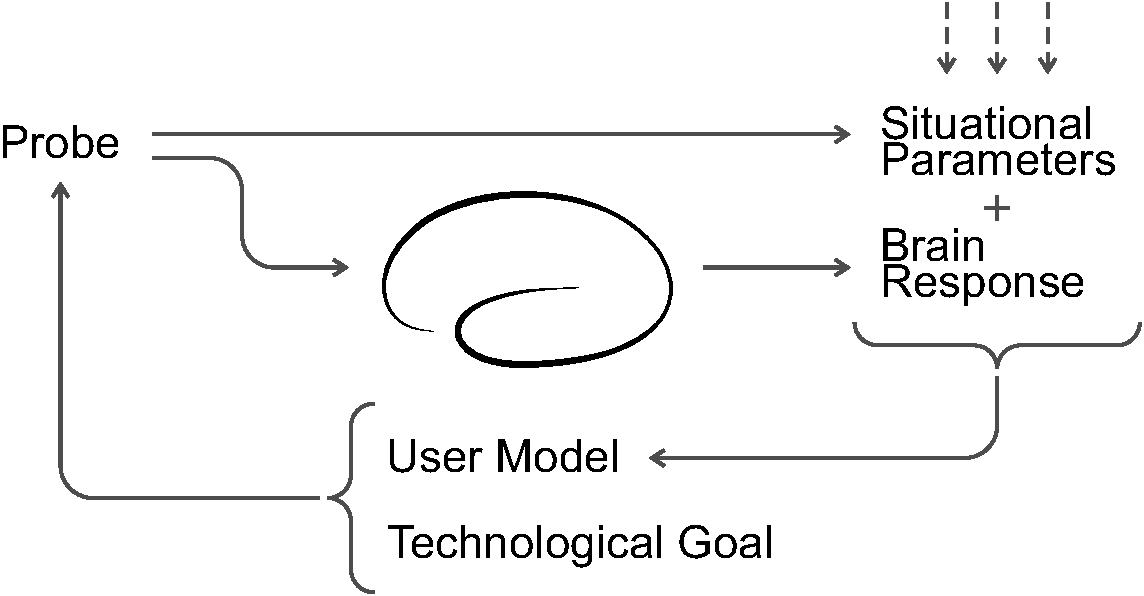
\includegraphics[width=10cm]{figures/cp-diagram.pdf}
    \caption[Diagrammatic overview of the cognitive probing mechanism.]{A diagrammatic overview of the cognitive probing mechanism. Based on available information, the technology initiates or manipulates a state change---a probe. This change elicits a brain response. Together with parameters describing the probe as well as, optionally, additional parameters describing the situation in which the user's response happened, the technology interprets this response and updates the model, increasing the accuracy of the information available to it for the next goal-oriented probe. At a minimum, the situation is described by the probe itself, but any other relevant parameters can be included.}
    \label{fig:cp:diagram}
\end{figure}

\paragraph{Summary.}
Figure~\ref{fig:cp:diagram} shows a diagrammatic overview of the cognitive probing mechanism. A probe elicits a certain response in the user's brain. The neuroadaptive technology measures this response, along with relevant parameters of the state change, and co-registers these pieces of information alongside one another in a user model. The combination of all pieces of information in the model allows inferences to be drawn. Based on the user model and the current goal of the technology, the next probe is initiated. This again elicits a response, leading to an update of the user model. 

To further delineate the method of cognitive probing, we mention a number of counter-examples in the discussion section of applications that are closely related to cognitive probing, but fall outside of this definition. For now, we will first turn to a number of past and present applications and experiments that do fit this definition, to illustrate the method.


\section{Literature Review}
\label{sec:literature}

The proposed definition of cognitive and affective probing is deliberately generic, and does not specify, for example, for what purpose the learned information is to be used, or how inferences are to be made. Therefore, we can identify a number of past and present methods that fit this definition. Although these methods have been treated disparately before, we can see that the same terminology applies.

We may say that the history of cognitive probing starts with the \emph{event-related potential} (ERP) technique \cite{luck2014erp}. This was the first of a number of techniques that allowed researchers to associate the brain's neuroelectric responses with specific events. Initially, the ERP technique was used both to elucidate the neural pathways involved in sensory processing \cite<e.g.,>{cobb1960erp}, and as a diagnostic tool to assess the (mal)functioning of the involved structures and processes \cite<e.g.,>{chiappa1997clinicalep}. Later, it was demonstrated that ERPs also reflect aspects of cognitive processing \cite{walter1964cnv}.

The ERP technique has been used in various applications and research endeavours. For example, \citeA{fischer1999mmncoma} used a mismatch negativity paradigm \cite{naatanen2007} to assess levels of consciousness in comatose patients, by presenting them with sentences that did or did not make semantic sense. \citeA{farwell1991gkt}, based on earlier work by \citeA{rosenfeld1988erpgkt}, presented participants with pictures of objects that did or did not belong to a crime scene in order to infer whether or not they had incriminating knowledge of it. 
Most ERP studies, however, including these two examples, do not employ automatic learning by the same computer that produces the stimuli, meaning they do not employ cognitive probing as such. Instead, the average ERPs are examined post hoc by the researchers. A key element that was missing was the ability to detect and analyse brain responses in real time. This had been demonstrated first in the 1970s \cite{vidal1977}, but resurfaced more prominently in the 2000s with the advent of machine learning in EEG research \cite{ramoser2000,blankertz2002singletrial,lotte2007classificationreview}. 

This development is clearly seen in reactive BCI applications \cite{zander2011}, where ERPs are elicited and used to assess correlates of human attention to allow users to voluntarily control applications. In particular, mental spellers highlight or present different letters of the alphabet on a display, in order to learn which letter was attended to \cite{farwell1988,treder2011gazeindepbci}. Each such presentation results in an ERP. Because ERP responses to attended letters are known to be different from those to unattended ones, the system can detect this in real time and learn which letter the user intended to write. These highlights and presentations are examples of cognitive probes: they are solely initiated for the purpose of learning which letter the user wishes to communicate. Later developments added adaptive probing techniques where the sequence of highlights was adapted in real time to the available information \cite<e.g.,>{lenhard2008adaptivep300,jin2011p300flashpattern}, or where intermediate feedback elicited additional brain responses \cite{dalseno2010}. Finally, \citeA{mladenovic2019activeinference} present an elaborate implementation of a mental speller that combines multiple adaptive strategies using a single framework based on active inference. Here, a prominent user model is used to generate the system's actions, the user's brain responses to which in turn are used to update that user model. This is a clear example of cognitive probing in the current sense of the term.

A similar development from independent analyses of brain activity to cognitive probing as described here happened in the field of neuroergonomics  \cite{parasuraman2003neuroergonomics}, where ERPs have been used for, among other things, workload detection. It has long been shown that certain features of brain responses to rare sound events seemingly reflect the availability of attentional resources \cite{sirevaag1989p300resource}. This led to the development of the secondary oddball task, where sounds are played repeatedly and intermixed with rare deviant sounds. Real-time evaluation of the brain responses to these tones then allow real-time inferences to be made with respect to available resources, i.e., workload. In such a context, the tones are thus cognitive probes, allowing the same technology that produces them to learn about the cognitive state of the user. This has been used in online, closed-loop contexts, where e.g. additional tasks are automated or postponed when high workload is detected in order to alleviate the load \cite{kohlmorgen2007}. Secondary oddball tasks have also been shown to work in demanding real-world scenarios \cite{dehais2018monitoringfatigue}.

In the previous examples, the state changes making up the probes were induced for the sole purpose of learning. However, this must not necessarily be the case: probes can also be embedded in state changes that are produced for other reasons. One example of this is the presentation of feedback in such a way as to elicit an error-related potential when the presented information is false or undesired \cite<e.g.>{dalseno2010}. Presentation of feedback is obviously an inherent part of any interactive system, its primary purpose being to 
inform the user. Its presentation can, however, be controlled by the computer allowing it to be used as a cognitive probe.

Similarly, \citeA{kirchner2016multirobotcontrol} effectively embedded a type of secondary oddball task in an otherwise natural human-computer interaction. During a multi-robot control task, participants had to pay attention to task-relevant messages that were presented during the interaction. The appearance of these messages evoked brain responses with properties comparable to those evoked by a dedicated secondary oddball paradigm. This allowed the computer to deduce an index of task engagement from these responses, and adapt the presentation of the messages-cum-probes accordingly. This shows that probes can be effectively hidden in natural aspects of an already-ongoing interaction.

It is even possible to have probes be the primary basis of the interaction. \citeA{zander2014implicit,zander2016nat} as well as \citeA{iturrate2015teaching} demonstrated applications where this was the case: the guidance of a cursor or a robotic arm, respectively. Each movement of the cursor or arm elicited an ERP that could be automatically interpreted as reflecting the appropriateness of that movement with respect to reaching a target position. The initial movements occurred randomly. Based on the information gathered from the observer's brain response following each movement, however, a dynamic user model could be generated reflecting which behaviours were perceived positively, and which were perceived negatively. Based on this model, the movements could be steered into the apparently desired direction, towards the target. While \citeA{iturrate2015teaching} suggest this to be used for voluntary prosthetic control, Zander \& Krol et al. (2016) stress that the elicited responses themselves appear to be involuntary. In fact, their participants were unaware of having any influence over the cursor. As such, this method allowed the cursor to be controlled entirely implicitly.

This latter example presents a sliding scale with respect to the primary purpose of each cursor movement. In a process later also described by \citeA{hincks2017entropicbci}, the stimuli were initially selected at random, with no other purpose than to populate the user model. As information was gathered and a user model was formed, the stimuli became increasingly part of the task completion (target reaching) mechanism while still allowing for new information to be learned.

A similar concept has been developed in the context of neuroscientific experimentation. Whereas traditional experiments are generally informed by specific hypotheses and employ correspondingly narrow experimental designs, a neuroadaptive approach to hypothesis testing would allow an experimental computer to present different stimuli or conditions in search for a specific neurophysiological response pattern \cite{lorenz2017neuroadaptivebayesian}. For example, in order to find which stimuli optimally activated select cortical regions, \citeA{lorenz2016automaticneuroscientist} used functional magnetic resonance imaging (fMRI) to assess the participants' responses to a range of audiovisual stimuli reflecting different physical properties. Rather than presenting all stimuli in order to analyse the different responses post hoc, responses were assessed in real time. Subsequent stimuli were automatically selected based on previously gathered responses, with the aim to learn the parameters that elicit a maximum response. This closed-loop, neuroadaptive experimental design thus employs cognitive probes in order to learn how the participant responds to certain stimuli. Once the optimal stimuli have been found, the experiment can continue to gather data for further investigation.

A final example concerns the generation of a dynamic user model reflecting user interests \cite{wenzel2017wordrelevance}. Here, the brain responses were not elicited by the presentation of the stimuli directly, but by the participant's eye fixation on them: the stimuli were already visible, the participants' gaze was tracked, and brain activity was analysed relative to the eyes fixating on each stimulus using so-called fixation-related potentials (FRPs; \citeNP{dimigen2011frp}). The stimuli were words of different semantic categories. By combining fixation information and an interpretation of the FRPs, the authors were able to assess which words were relevant and which were not, and ultimately, to infer which category of words the participant was interested in. This illustrates that the brain response to a specific probe (presenting the words) need not be immediate, but can be delayed. In this case, it was delayed until the participant fixated on it. This also illustrates the potential relevance of additional context information. \citeauthor{wenzel2017wordrelevance} combined the brain response with information about the participant's gaze in order to infer the semantic category of current interest.

Aside from fMRI and the EEG-based ERP technique, which featured heavily in this section, frequency-based measures can of course also be used \cite<e.g.,>{ewing2016tetris,mousavi2017mi}, as well as other modalities, such as functional near-infrared spectroscopy (fNIRS) \cite<e.g.,>{afergan2014dynamicdifficulty,yuksel2016bach}. 

In these examples from different areas of research, we see a convergence towards the idea of using real-time, single-trial analyses in an automated, closed-loop fashion in order to learn something about the human user or participant---i.e., towards the idea of cognitive probing presented here. While clearly sharing common methodologies, the used terminology is still disparate: authors referred to their methods, or parts thereof, as ``probing'' (\citeNP{kane2000erpcoma}; Zander \& Krol et al., 2016), ``brain reading'' or ``embedded brain reading'' \cite{kirchner2019embeddedmmi}, ``exploration'' \cite{iturrate2015teaching}, ``active sampling'' \cite{lorenz2017neuroadaptivebayesian}, ``active inference'' \cite{mladenovic2019activeinference}, or implied the method to be part of an ``entropic BCI'' \cite{hincks2017entropicbci}, of ``adaptive'' systems \cite{schultheis2004textdifficulty,yuksel2016bach}, or of a system using ``brainput'' \cite{solovey2012brainput}. This is part of the reason why we now present a unified framework and terminology.

In the next section, we discuss a number of aspects of cognitive probing that determine how implementations may differ, and aspects that are important to consider when developing systems that employ this method. In some cases, these overlap with general active learning aspects and guidelines; in others, cognitive probing must be treated separately due to its utilisation of brain data gathered directly from human beings.


\section{Aspects and Considerations}
\label{sec:aspects}

Cognitive probing can be applied in different ways and across different contexts, to suit different purposes. This section lists a number of ways in which these differences can be realised. This serves both to illustrate concepts, techniques, and possibilities of the cognitive probing method, and as a list of considerations and trade-offs for researchers and developers.

Furthermore, the cognitive probing method raises a variety of ethical issues that we will briefly introduce and discuss in this section. The basic concern centres around the implications of probing someone's brain processes in order to gather cognitive or affective information about that person. A responsible use of such technology requires, at the very least, reflections on the topics of privacy and consent, and responsibility for actions mediated by the technology. 


\subsection{Learning Strategies}
\label{sec:strategy}

Probes are designed in order to obtain information. Two central questions are thus: What information is to be obtained, and how is this best achieved?

Ultimately, the information that can be obtained of course depends on the cognitive and affective states that can be detected and the reliability of these assessments. Here, traditional neuroscientific considerations apply. See e.g. \citeA{brouwer2015pitfalls} and \citeA{gerjets2014workload} for recommendations.

There are different possible strategies to learn from cumulative samples and to choose subsequent probes. In the previous section, \citeA{lorenz2016automaticneuroscientist} and \citeA{mladenovic2019activeinference}
used Bayesian inference and optimisation \cite{snoek2012bayesianoptimization}, whereas \citeA{iturrate2015teaching} used a form of reinforcement learning \cite{sutton1998reinforcementlearning}. 

With its abstract similarity to active learning, the cognitive probing method can utilise many of the so-called query strategies of active learning \cite{settles2009activelearning}. As illustrated in Figure~\ref{fig:cp:diagram}, the system can select a specific state change based on the knowledge currently available in its model, in order to update that model (i.e., to fulfil its goal of learning). It can thus use available information in order to determine which change will be initiated, and to what end.

One strategy to that effect that \citeA{settles2009activelearning} mentions is \emph{uncertainty sampling}: the system can initiate changes along those dimensions about which it has the least knowledge. For example, if the system has no information pertaining to a particular condition, it could deliberately produce this condition in order to probe the user's response to it. 

Other strategies can similarly be applied, notably \emph{expected model change} (obtaining information that would most change the model) and \emph{expected error reduction} (to reduce the error in the model, or in the system's behaviour). A system may initialise using random variables and based on these initial samples, move to specific strategies to find more suitable values \cite{hincks2017entropicbci}.


\subsection{Repeating Probes}

Most likely, it will be necessary to probe multiple times in order to draw reliable conclusions. Given imperfect measurement or inference methods, a trade-off needs to be considered between the number of probes and the accuracy of the gathered information.

With respect to obtaining a specific piece of information, a sequence of probes can be presented in different ways. One way is to present a precisely defined state change a pre-determined number of times (e.g., once, or ten times). The optimal number of repetitions has, for example, been investigated for P300 spellers \cite<e.g.,>{jin2011p300flashpattern}. Another method is to use a confidence criterion, where the state change is repeated until a certain level of confidence has been reached (i.e., the error reduction strategy combined with dynamic stopping; \citeNP<e.g.,>{schreuder2013dynamicstopping}). Finally, rather than repeating the same probe, the probe itself could be dynamically changed during the sequence, adaptively homing in on increasingly specific information of interest as e.g. in \citeA{lorenz2017neuroadaptivebayesian}. 


\subsection{The Roles of Time}

Time is relevant in a number of ways. For one, time itself may be one of the relevant situational factors to be included in a model: the absolute time of day (e.g., to learn patterns that are different in the evening as compared to the morning), or the time relative to a previous event.

Also the time needed for the system to measure and process the brain response can have practical importance. Sometimes the measurement and data analysis might take longer than what is useful for a particularly time-critical application.

Furthermore, the duration of a probe's effect needs to be considered. In the examples given in this paper so far, all relevant brain responses to the probe were near-immediate. However, this need not always be the case. Depending on the application, a distinction can be made between up to four time points or periods: the time that the probe is generated (i.e., the technological state is changed); the time that the probe is perceived; the period of time during which the probe's influence remains apparent (i.e., during which relevant brain responses can be gathered); and the period of time during which the gathered information remains valid.

The first two time points are usually the same, but not necessarily. It is possible for a probe to be noticed only after it has been produced, as for example in the fixation-related study mentioned above \cite{wenzel2017wordrelevance}. It may also be possible for a state change not to be consciously noticed at all, while still having an effect \cite{negri2014subliminal}. The third point covers a time period that varies depending on factors such as habituation, and the time it takes for a meaningful response to arise---see also section~\ref{sec:impulsive} for the difference between impulsive and reflective responses. The final point concerns the ``half-life'', so to say, of any gathered information. Is it generally valid and can it remain in the model indefinitely, or may the user's responses change over time such that the learned information becomes obsolete? In the latter case, the probes may need to be repeated at certain intervals.


\subsection{A Probe's Purpose}
\label{sec:purpose}

The presented definition requires that probing must be done in order to learn. This does not mean, however, that learning is necessarily the only objective: the system may simultaneously have other goals.

Figure~\ref{fig:cp:diagram} illustrates three effects of a probe: its effect on the environment (at a minimum, this is simply the occurrence of the probe itself), its effect on the brain (the brain response elicited by the probe), and ultimately, the adjustment of the model. The goal of ``learning'' refers to this last effect. However, cognitive probes can be selected to simultaneously fulfil further strategic goals. In particular the second consequence, the user's response, can be part of the goal-driven behavioural strategy of the system.

The system may aim to induce or sustain desirable psychophysiological user states. If certain probes have been learned to lead to positive responses, the system may aim to induce or sustain the user's positive state by repeating such probes. This was the case for the implicit cursor control experiment (Zander \& Krol et al., 2016): each probe served both to further the system's knowledge of the preferred direction, and to steer the cursor into that direction.

Note that goals need not remain static over time: for example, an initial phase of mere information-gathering can be followed by different goals as decided based on the gathered information, or goals may change based on changing situational aspects.

Furthermore, even when learning is the main objective to employ cognitive probing itself, the purpose for which information needs to be learned is left entirely open.

In other words, it can be said that neuroadaptive systems have their own agenda \cite{fairclough2017intadapt}. An important factor to consider is whether or not, or to what extent, this agenda is in line with the user's own goals, discussed in more detail further below.


\subsection{Interference and Distraction}
\label{sec:interference}

The fact that cognitive probes are intended to elicit a response means that they must influence the user in one way or another. As mentioned above, this influence can be used by the system for a higher goal, such as the promotion of a desired mental state. At other times, this influence may be an unwanted side-effect. The effects may be distracting or otherwise bothersome, in particular when the system does not yet have a sufficiently accurate model, or when probes are selected using a seemingly incomprehensible strategy. Potentially, this could even influence their mental state to a point of no longer being useful as implicit input.

In utilising cognitive probes, it must be considered to what degree these probes may interfere with the user's natural or intended behaviour. An important factor here is how well the probes can be embedded into the natural context.

For example, the secondary oddball tasks mentioned earlier used clearly perceptible, overt auditory probes \cite{schultheis2004textdifficulty,kohlmorgen2007}. These were required in order to learn of the user's attentional resources, but were otherwise irrelevant to the user. These are inherently distracting stimuli \cite{parmentier2011distraction}. On the other hand, the example of task-relevant messages that were co-opted as probes \cite{kirchner2016multirobotcontrol} shows that they may have been distracting, but not because they were probes---their use as probes did not change their nature as part of the interaction. The messages themselves were clearly perceptible, but their function as probe was not noticeable at all. This can also change over time. During the cursor and robot control examples (Zander \& Krol et al., 2016; \citeNP{iturrate2015teaching}), the initial actions were purely information-gathering probes, but later actions, based on an increasingly accurate model, were increasingly compatible with the user's goals, and their probing nature became secondary to the goal of steering the cursor to the target. 

Probes that are embedded in naturally-occurring events are less distracting, but must wait until those events happen. Also note that, the better probes are ``hidden'', the more care must be taken not to violate the user's privacy, discussed in section~\ref{sec:privacy}. Alternatively, a user can be exposed to a calibration phase of clearly perceivable and attended, but seemingly unproductive probes until the model is sufficiently accurate for the probes to be helpful. In other cases, of course, e.g. where the process always has the full attention of the user, these deliberations may not apply.


\subsection{Representing Multiple Dimensions}
\label{sec:dimensionality}

Theoretically, the model that contains the gathered information can be of any level of complexity or dimensionality. Not only can any number of probe-response events be taken into account, any number of additional context measurements can be registered along with that response.

Most applications can be broken down into discrete dimensions: a light, for example, may be determined by its hue and its intensity. Cognitive probes could be used to gather a person's current preference with respect to these two dimensions. However, such preferences may be dependent on further dimensions: the time of day, their current activity in the room, whether or not there are guests... In this sense, the full complexity of the real world has an indeterminate number of dimensions.

Each probe can be seen as a single point in a large state space covering all dimensions in the model. Section~\ref{sec:strategy} already covered some strategies to explore this space. An additional consideration is the desired accuracy on each individual dimension. Disentangling the contributions of individual dimensions will require a large amount of probes, and until such time, no meaningful inferences can be drawn.

Alternatively, the complexity may be increased step-wise, with additional dimensions added only in due time, after prior models have been properly calibrated. We may also note that not all information must necessarily be obtained through cognitive probing. One could pre-populate a user model with expected values, and have the system select cognitive probes using expected model change strategies to quickly adapt the model to the momentary preferences of the individual user. Similarly, multiple archetypal user models might be pre-populated, e.g. using statistical inference based on large amounts of data, and cognitive probes can be used to select between them for any given moment or person. 


\subsection{Impulsive versus Reflective Responses}
\label{sec:impulsive}

Because cognitive probing relies on externally induced brain responses, rather than self-initiated responses, it is possible that these responses are the result of shallow (impulsive, intuitive, reflexive) processing, subject to heuristics and biases \cite{kahneman2011fastslow}. In that case, it is important to know to what extent the induced brain responses (would) correspond to explicitly given responses.

Refer, for example, to \citeA{frankfurt1971}'s distinction between first- and second-order volitions, where first-order volitions reflect first impulse desires (e.g., wanting to smoke a cigarette), while second-order volitions (wanting to stop smoking) reflect our self-control, reason-based cognition. It is conceivable that a person, given the time to deliberate and formulate an explicit response to a probe, would come to a different one than the one induced and inferred by the technology. As such, cognitive probes could result in information being implicitly communicated by the user that the user does not or would not authorise. 

Cognitive probing does not prescribe using either impulsive or reflective brain response. It is, however, an important distinction for researchers and developers to be aware of, as it concerns the type of information that can be learned using cognitive probes in different contexts, and the extent to which this information and subsequent adaptations may be accepted by the user. Furthermore, this can have profound effects on responsibility assessment, discussed next.


\subsection{Outcome Responsibility}

Who or what is responsible for an outcome that is based on cognitive probing? As mention in section~\ref{sec:purpose}, the technology acts upon the information it gathers by modulating future probes in order to learn, but it can also use that information to execute different, additional actions. 

When technology contributes autonomously to the performance of a task a user is engaged in, it may become difficult to separate the two interacting agents. How would the user (or others) evaluate the respective contributions of human and technology? By whose authority is an action executed? To whom would ``ownership'' of the action be ascribed, or responsibility for its outcome? Even while performing an action, the users themselves might be uncertain about being the (only) agent of an action \cite{haselager2013agency}, with systems that make autonomous decisions additionally decreasing the users' own autonomy \cite{friedrich2018bciautonomy}.

Because cognitive probing relies on externally induced brain responses, one could argue that behavioural outcomes based on this information would fall within the reflexive or spontaneous behaviour class, or at least that the underlying thought process was not finished (see also section~\ref{sec:impulsive}). Users could attempt to disavow such behaviours as not being congruent with their own reason-based ideas about how they ought to act. Users who do not agree with (the use that is being made of) their own brain responses may argue that responsibility lies elsewhere, since their input to the system bypassed their conscious awareness and control.

Moreover, probing technology might lead to a situation where users could reasonably feel that in cases of continuous deepening probes (probes provided on the basis of cognitive information gathered from previous probes), their capacity to engage in autonomous reasoning and decision making may be compromised. In essence, one needs to consider the implications of ``nudging'' technology being applied at the level of brain processes, opening up further possibilities for user manipulation (see also section~\ref{sec:purpose}).

There are different types, or ways of claiming, ownership of action. Under normal circumstances we accept our actions to be ours, irrespective of whether they were of a reflexive nature, spontaneous first impulses, or following deliberation. However, when it comes to assessing the moral consequences of such behaviours, we may differentiate between them. The assessment of my responsibility, e.g. my guilt, based on my behaviour that led to damage, e.g. a broken glass, may differ depending on whether my behaviour was a mere reflex, a spontaneous movement, or a consequence of a reasoned judgement.

Under such circumstances, it seems possible that users will ``blame'' the technology in cases with negative outcomes, but praise themselves in cases of success. 

The effect of cognitive probing on assessing the responsibility for consequences in legal or financial contexts will be far from straightforward. Presumably, many of such consequences could be dealt with by using liability waivers, although this could affect the willingness of users to accept cognitive probe technology in realistic contexts (with realistic consequences). Also note that procedures and criteria for accepting or attributing responsibility may diverge significantly between legal, and moral domains. It is important that researchers and designers of systems with direct access to brain activity and the ability to act autonomously ensure that they act with the user's permission and in accordance with the user's wishes \cite{fairclough2009fundamentals,mecacci2019criteria}. 


\subsection{Privacy and Consent}
\label{sec:privacy}

The interference discussed in section~\ref{sec:interference} referred to the immediate intrusion that individual probes could pose into a user's state of mind. The method of cognitive probing in general, however, could also be understood to intrude more fundamentally into a person's privacy, as it elicits and utilises brain responses that are beyond the direct control of the user. As such, cognitive probing allows technology to autonomously gather or ``extract'' information from the user, touching upon the privacy of thought. As discussed above, this information gathering can potentially take place unbeknownst to the user---and thus, potentially, without consent. 

Therefore, care must be taken that the data is handled with proper care for the user's privacy and the security and confidentiality of all gathered data \cite{fairclough2014confidential}. Brain data in particular, being more closely connected to the privacy of ``inner'' thoughts and feelings, may be all the more sensitive. Moreover, by utilising automatic brain responses, the information acquired may reflect mental features that, to some extent, remain out of reach of a person's self-control, meaning data may be gathered that would not have been voluntarily provided, or would not even be known by the users themselves.

Hence, users of cognitive probing applications should be given full transparency: they should be informed clearly and unequivocally about the nature, methodology, and aims of the technique (see also \citeNP{ienca2018brainleaks}). Specifically for cognitive probing technology, at the very least, they should be informed that \emph{a)} cognitive probes induce brain responses that the users normally cannot suppress, \emph{b)} such probes and responses can and will be used to gather information about the user's cognitive and affective states, and that \emph{c)} this information, in addition to contextual information that is also being gathered, will be used to provide more and possibly better directed probes in order to extract even more information.

\citeauthor{haselager2018reading} (2018; see also \citeNP{mecacci2019nta}) discuss applications of brain measurement aimed at brain reading, i.e., decoding mental content. This discussion applies to cognitive probing as well, as both methods capture cognitive information. They suggest that two factors are of vital importance with respect to potential abuse: concealability, and enforceability. 

Concealability indicates the extent to which a user can be left unaware of the actual goals behind the particular application, e.g. the nature, amount, or detail of the cognitive or affective states that are being explored. Note that the mere knowledge that one's brain states are being monitored and probed does not imply an awareness of which aspects of cognition are being investigated.

Enforceability is related to the extent to which the application is resilient to a subject's voluntary attempt to disrupt the process. In the current context, this implies that once subjects are participating in the process, the more ``automatic'' their responses to a probe are, the more enforceable the information gathering will be. 

Consideration of these two factors leads to the further requirement that \emph{d)} users will be informed about the exact nature, amount, and detail of the information about cognitive and affective states explored, with in addition \emph{e)} the purposes for which this information is being gathered. 

Given the sensitive nature of such gathered information, \emph{f)} procedures and guarantees regarding the ownership of data should be installed ensuring that users of cognitive probing applications remain in control of the data acquired, its storage, and its future use \cite{fairclough2014confidential,yuste2017ethical}. As one part in safeguarding the users from the above issues, \emph{g)} the user must have access to a comprehensive and meaningful representation of all information in the model, and insight into the logic of the system's probes and model-based behaviour, in line with the recent General Data Protection Regulation (GDPR) of the European Union \cite{eu2016gdpr}.

However, it is not only brain-related information, or its interpretation in mental terms, but also the ensuing operations of the technology that might constitute threats to (mental) privacy of its users. Probe-based technological state changes may lead to publicly noticeable outcomes that, even when in agreement with a user's genuine preference, may be socially problematic or undesirable. At the very least, therefore, \emph{h)} users should be aware that aspects of their mental states may be revealed to outsiders in the form of probes or other adaptations.

Of course, we do not wish to claim that this list of requirements is complete or formulated precisely enough. Moreover, the stringency with which they should be applied will depend considerably on the context and purposes of the applications. However, cognitive probing does pose serious threats to privacy and consent, and this section specifies a number of concerns which researchers and developers are called on to consider and discuss.


\section{Discussion}
\label{sec:discussion}

Cognitive probing combines the ability of technology to interpret ongoing measures of arbitrary brain activity, with the ability of that same technology to actively and purposefully elicit cognitive and affective responses from its users. This is used to learn and infer information from these responses. Based on the resulting knowledge, additional, increasingly targeted responses can be elicited.

Looking at the different commercial, clinical, and experimental approaches and applications mentioned in section~\ref{sec:literature}, we believe the concept of cognitive probing as introduced here describes the fundamental similarity between a number of previously separate endeavours. Some early incarnations date back to decades ago, but along with an increasing ability to automatically assess and interpret mental states has come an increasing number of recent, novel examples that fit this same definition of cognitive probing. Some stem from strictly controlled laboratory environments, but given the current commercialisation of neuroadaptive technology, a growing number of examples are now also preparing for general use. Going forward, it is important to recognise the fundamental similarities shared by these different applications, especially since the specific configuration that defines cognitive probing gives rise to a number of serious ethical considerations.

To further delineate the concept of a cognitive probe, we now consider some counter-examples that deviate from the definition in specific ways. Without implying that less care should be taken in these cases, the following examples do fall outside of the specific scope of cognitive probing.

As one example, we may consider a case where all other requirements are met but the response-eliciting event in question was not influenced by the system at all, i.e. it was not initiated or manipulated by it. For example, instead of a radio being switched on, a colleague starts whistling a tune. A context-aware system may still register this, identify it as a noteworthy event, record the listener's brain response to it, and infer whether or not this tune is distracting. Since the colleague acts independently, it cannot be said that their behaviour is a probe from the system.

When the state change is not independent from the technology, a crucial question becomes what exactly counts as being ``initiated'' or ``manipulated'' by it. A text message that you receive on your phone was initiated by the sender, but the notification you receive of it may not have been, depending on how your phone handles notifications. If the phone is programmed to always automatically immediately notify you of all messages that come in, the phone has no control over them and they should be seen as being initiated by the sender of those messages. If your phone does have policies in place that allow it to manipulate the notifications, they can be used as cognitive probes. 

Of course a neuroadaptive system may use any and all information available to it, including all responses to external or otherwise non-probe events. Doing so, however, would not necessarily constitute cognitive probing, but more generally the collection, selectively or indiscriminately, of event-response samples. 

As another counter-example, a system may have access to a measure of its user's brain activity and initiate a state change to get a specific response---but without learning from it. Instead, it could be initiated for the sake of the response itself. A car detecting a state of drowsiness in its driver may decide to sound an alarm in order to awaken the driver. This would be a state change initiated by the car designed to elicit a specific response from its user, but it would not be a cognitive probe as the loop is not closed and no information is retained.

Other brain responses may not contain any cognitive or affective information per se. BCI systems relying on steady-state visually evoked potentials (SSVEPs; \citeNP{middendorf2000ssvepbci}) for example, make use of the fact that when a human is presented with a visual stimulus that is flashing at a specific frequency, their visual cortex will exhibit neuro-electric activity at that same frequency (and its harmonics). When different stimuli thus flash at different frequencies, the dominant frequency in the visual cortex can reveal what stimulus a user is looking at. Thus, SSVEP-based BCI systems present system-controlled state changes (the flashing of the visual stimuli), monitor the user's brain response to these state changes, and infer from the found frequency which letter the user was looking at (i.e., wanted to select). This is not cognitive probing, however, as the brain response in question is not related to the user's cognition. The activity in the visual cortex is a direct result of the sensory input; there is no relevant top-down cognitive influence. This separates this method from e.g. attention-based mental spellers, where cognition does influence the measured response. Furthermore, these applications tend to be one-shot approaches with no model learning.

Finally, not all closed-loop neuroadaptive systems \cite{krol2018interactivity} use cognitive probing. Adaptive automation, for example, adjusts automation levels based on a measurement of workload in order to keep this workload within a desired range \cite{byrne1996adaptiveauto}. This principle has also been used to make sure students sustain an adequate level of engagement \cite{yuksel2016bach}. Here, when a measure of load surpasses a certain threshold, the technology changes the conditions by e.g. increasing or decreasing automation, or presenting material at an appropriate level of difficulty. These changes are designed to influence the user and maintain a desired psychological state. When, following this, the measure again passes the threshold, further adjustments are made. This method has many aspects in common with cognitive probing, but these examples do not employ a model where responses to specific conditions are saved. These systems demonstrate the idea that directed adaptations based on an ongoing evaluation of a user's state can influence that same state, but they stop short of using that influence and evaluation to automatically learn from the effects of such adaptations---although they could easily be extended to do so.

As mentioned before, examples or forerunners of cognitive probing can be found going back decades, with similar developments happening in parallel. This has resulted in essentially equivalent approaches being developed independently, and being given separate names. In our proposed unification, we elected for the label ``cognitive probing'', or ``affective probing'', as \emph{probe} was one of the first terms that was and still is being used for computer-presented stimuli aimed at eliciting specific brain responses \cite{kane2000erpcoma,espie2007insomnia,lawrence2014}. We must note that the same term has found some use also in the fields of questionnaire design, where it refers to follow-up questions targeting specific previous statements \cite{beatty2007coginterview}, and in psychotherapy, where a cognitive probe may be such a question as ``What are you thinking right now?'' \cite{beck1991cognitivetherapy}. The semantic overlap here, we believe, does not interfere with the more specific meaning in the context of neuroadaptive technology, but rather demonstrates that this term readily reflects important parts of the intended meaning.

Cognitive probing represents only a specific method in the larger field of neuroadaptive technology, but it is a powerful one. It allows neuroadaptive technology to escape the confines of a single cybernetic loop \cite{pope1995biocybernetic}, and, in effect, allows it to autonomously pose questions to the user, obtaining an implicit answer directly from the user's elicited brain activity. Why it asks those questions and what it subsequently does with the answers---the options are innumerable.


\section{Outlook}
Traditionally, machines only respond to their operators' explicit commands. Using passive brain-computer interfaces and further forms of physiological computing, it is possible to incorporate automatic interpretations of user states as secondary input modalities. With cognitive probing, it is possible to not merely rely on the naturally available information, but to actively and autonomously gather information that was not otherwise available from the user---potentially even unbeknownst to them. 

The example of a neuroadaptive book, described by Zander \& Krol et al. (2016), provides an interesting hypothetical scenario for cognitive and affective probing:

\begin{quote}
While reading, the reader would interpret the story as it unfolded, thus automatically responding to events with a detectable affective state. Based on what the reader apparently finds enjoyable, a neuroadaptive system could then change the content of subsequent pages. With a sequence of such adaptations, the story is gradually steered in the reader's preferred direction. However, the reader would not actively be directing the story, and would not even need to be aware of the system's existence. (Zander \& Krol et al., 2016)
\end{quote}

Interactive narratives using neurophysiological input have been presented before \cite{gilroy2013bcinarrative}, but none where the events unfolding on the pages serve both as the content of the book, and as probes. They are neither distracting nor intrusive, as they are perfectly embedded into, in fact \emph{are}, the story itself. The first few chapters may be pre-determined, designed to learn the reader's attitudes towards, say, the main characters. Should, however, this not suffice, the book could decide to present the reader with another chapter focusing more thoroughly on the one character it is least certain of (i.e., uncertainty sampling).

In this example, the complexity of the model depends largely on the amount of possible paths the book will have. It could be merely a decision between two outcomes, or more complex information can be gathered to allow more detailed plot developments and twists. In an extreme case, language models may be used to generate new paragraphs and adaptive probes for an intricate model and potentially endless storyline \cite{radford2019language}. The purpose of the book as a whole could be, for example, to provide a pleasant experience (sustain a positive psychological state), to induce as many surprising plot twists as possible, or even to reveal deep, personal values.

Either way, the final contents of the book will at least partially reflect the reader's brain responses. The example thus also makes it clear how the very behaviour and outcome of a neuroadaptive system may reveal sensitive information, as discussed in section~\ref{sec:privacy}. While cognitive probing-based neuroadaptive systems allow for a unique level of personalisation, would the reader wish to reveal to others that, for example, evil prevailed in their version of the book? 

An illustrative use case for non-embedded cognitive probing may be found with online retailers. After selecting a category, a number of stock items may be presented and the user's reaction probed, until a recommendation is made tailored to the user's inferred preferences.

Here, it is obvious to the user that they are being probed, and for what purpose. In the case of the neuroadaptive book, it may be altogether unclear which parts of the rich prose exactly comprise the probes and what information they attempt to gather. We emphasise the ethical issues mentioned in section~\ref{sec:aspects}, in particular concealability and transparency.

In theory, a neuroadaptive system can be imagined in a ubiquitous computing approach, i.e., with access to a large amount of context information concerning the user's many everyday interactions with their environment. If even a single cognitive user state---positive versus negative, satisfaction versus dissatisfaction---could be accurately inferred and co-registered with these many interactions and other context information, a user model could be generated that, over time, could contain a very detailed description of this user's habits and preferences. Cognitive probes may be used to expand this user model with increasing efficiency. A system that continuously learns from our implicit responses to its directed probes, and thus generates a rich understanding of our preferences and intentions, may even be in a position to exhibit a form of intelligence and empathy, and support us in a way not currently possible by robots or other machines. 

From a different angle, such a system might also be used as a tool to influence the cognition and the mindset of a person in an interplay between the probes' ability to obtain information and its ability to produce specific responses. Imagine a (social) media platform with access to brain activity, where each presented piece of media could constitute a probe. Even inferences of seemingly simple information---for example, colour preferences in order to adjust the interface's colour scheme---could be used in potentially dangerous ways: politicians of different parties could be deliberately presented with different background colours, biasing the user to dislike the politician presented outside of the preferred colour scheme under the guise of advertisement personalisation. Cognitive probes may also be capable of assessing political preferences directly. With cognitive probing's ability to obtain increasingly specific information and target specific cognitive or affective functions, even outside of the user's awareness, it may simultaneously produce increasingly subtle methods of manipulating the user's mindset. We mention this example to again highlight the importance of consent and transparency.

A number of aspects and considerations mentioned in section~\ref{sec:aspects} remain open to investigation. Can we distinguish between impulsive and reflective responses? To what extent are they different, neurophysiologically and behaviourally? Which ones could be targeted using what probes? How do users judge agency and responsibility in different cognitive probing cases? What influences this? What are potential consumers' attitudes towards cognitive probing from e.g. a privacy standpoint? Answers to such questions will help determine what can and cannot, and what should or should not be achieved using cognitive and affective probes.

Going forward, provided that researchers and developers properly discuss and address these and other serious ethical concerns, we believe that cognitive probing can help make technology more intelligent, more interactive, and more adaptive to their users' needs and preferences.


\section*{Acknowledgements}

Part of this work was supported by the Deutsche Forschungsgemeinschaft (ZA 821/3-1).


\section*{References}

A shared bibliography starts at page~\pageref{bibliography}.


\clearpage
\pagestyle{plain}

        
    \part{Tools}
    \label{part:tools}
        
\chapter{SEREEGA: Simulating Event-Related EEG Activity}
\chaptermark{SEREEGA}%
\label{chapter:sereega}%


{\chaptermeta 

\textbf{Krol, L. R.\textsuperscript{1,2}, Pawlitzki, J.\textsuperscript{1,3}, Lotte, F.\textsuperscript{4}, Gramann, K.\textsuperscript{2,5,6} \& Zander, T. O.\textsuperscript{1,2,3}}

{\small
\textsuperscript{1}Team PhyPA, Biological Psychology and Neuroergonomics, Technische Universität Berlin, Berlin, Germany
\textsuperscript{2}Biological Psychology and Neuroergonomics, Technische Universität Berlin, Berlin, Germany
\textsuperscript{3}Zander Laboratories B.V., Amsterdam, the Netherlands
\textsuperscript{4}Inria, LaBRI (CNRS/University of Bordeaux/Bordeaux INP), Talence, France
\textsuperscript{5}Centre of Articial Intelligence, School of Software, Faculty of Engineering and Information Technology, University of Technology Sydney, Sydney, Australia 
\textsuperscript{6}Center for Advanced Neurological Engineering, University of California San Diego, San Diego, USA

This is the postprint version of the manuscript published as follows:

Krol, L. R., Pawlitzki, J., Lotte, F., Gramann, K., \& Zander, T. O. (2018). SEREEGA: Simulating event-related EEG activity. \emph{Journal of Neuroscience Methods, 309}, 13-24. doi: 10.1016/j.jneumeth.2018.08.001\nocite{krol2018sereega}
\par}}


\abstract%
\emph{Background:} Electroencephalography (EEG) is a popular method to monitor brain activity, but it is difficult to evaluate EEG-based analysis methods because no ground-truth brain activity is available for comparison. Therefore, in order to test and evaluate such methods, researchers often use simulated EEG data instead of actual EEG recordings. Simulated data can be used, among other things, to assess or compare signal processing and machine learning algorithms, to model EEG variabilities, and to design source reconstruction methods. \emph{New method:} We present SEREEGA, \emph{Simulating Event-Related EEG Activity}. SEREEGA is a free and open-source MATLAB-based toolbox dedicated to the generation of simulated epochs of EEG data. It is modular and extensible, at initial release supporting five different publicly available head models and capable of simulating multiple different types of signals mimicking brain activity. This paper presents the architecture and general workflow of this toolbox, as well as a simulated data set demonstrating some of its functions. The toolbox is available at \href{https://github.com/lrkrol/SEREEGA}{https://github.com/lrkrol/SEREEGA}. \emph{Results:} The simulated data allows established analysis pipelines and classification methods to be applied and is capable of producing realistic results. \emph{Comparison with existing methods:} Most simulated EEG is coded from scratch. The few open-source methods in existence focus on specific applications or signal types, such as connectivity. SEREEGA unifies the majority of past simulation methods reported in the literature into one toolbox. \emph{Conclusion:} SEREEGA is a general-purpose toolbox to simulate ground-truth EEG data.


\clearpage


\fancypagestyle{sereega}{%
    \fancyhf{}
    \fancyhead[EC]{\textit{\leftmark}}
    \fancyhead[OC]{\textit{\rightmark}}
    \fancyfoot[C]{\thepage \\ \vspace{9.9mm} \colorbox{footerbg}{\parbox{\paperwidth-2\fboxsep}{\centering\parbox{0.75\paperwidth}{\centering\fontsize{9pt}{9pt}\selectfont\textcolor{footerfg}{This is the postprint version of published manuscript: Krol, L. R., Pawlitzki, J., Lotte, F., Gramann, K., \& Zander, T. O. (2018). SEREEGA: Simulating event-related EEG activity. \textit{Journal of Neuroscience Methods, 309}, 13-24.}}}}}
    \fancyfootoffset[]{1.25in}}
\pagestyle{sereega}


\section{Introduction}

Having seen almost a century of continuous research and development since its first application on humans in the 1920s \cite{berger1929humaneeg}, electroencephalography (EEG) is now widely used in, among others, clinical settings, neuroscience, cognitive science, psychophysiology, and brain-computer interfacing, while its use continues to expand in fields such as neuroergonomics \cite{parasuraman2007neuroergonomics,frey2016eegux}, neurogaming \cite{krol2017meyendtris}, neuromarketing \cite{vecchiato2011eegmegmarketing}, neuroadaptive technology \cite{zander2016nat} and mobile brain/body imaging \cite{gramann2011mobireview}. As of December 2017, PubMed reported over 140~000 publications related to EEG, with over 4~000 published in each of the past five years.

EEG reflects the electric fields that arise primarily due to the synchronous activity of post-synaptic potentials at apical dendrites in the cortical surface of the brain, as recorded by electrodes placed on the scalp. As such, it measures a specific subset of brain activity. This enables cognitive and affective correlates to be found in the EEG, allowing post-recording or even real-time evaluation of certain mental states exhibited by the recorded person, such as surprise \cite{donchin1981}, error perception \cite{falkenstein1990,blankertz2002}, task load \cite{klimesch1999eeg,muhl2014crosscontextworkload,zander2017surgery}, or imagined movement \cite{pfurtscheller2001motorimagery,blankertz2007}. Compared to other brain monitoring and imaging methods, EEG is relatively inexpensive and provides a high temporal resolution. It is also becoming increasingly portable and ready for personal use \cite{zander2017dry} in various forms of neuroadaptive technology \cite{krol2018interactivity}. This explains EEG's relative popularity.

However, these advantages present a trade-off, with costs incurred primarily in spatial resolution. A single electrode records the average activity of up to a billion neurons, and probably never less than 10 million neurons \cite{nunez2006eegneurophysics}. This and other issues including volume conduction, the placement and distance of the electrodes relative to the cortical generators of the activity they measure, and the complex relation between cortical functions and features of scalp potentials, require that great care is taken when analysing and interpreting raw EEG recordings.

A host of methods have been developed over the last decades to extract robust features from the recorded EEG that correlate to cortical functions and can be understood in a neurophysiological or statistical sense. Examples are the event-related potential technique \cite{luck2014erp}, independent component analysis \cite{makeig1996}, common spatial patterns \cite{guger2000csp}, hierarchical linear modelling \cite{pernet2011limo}, and a many signal processing and machine learning algorithms \cite{lotte2007classificationreview}.

One major difficulty in developing techniques for EEG analyses is that there is no \emph{ground truth} that describes the exact brain activity: The recorded EEG data cannot be compared to the actual neuro-electric activity of the brain because no technique exists to provide such a reference measurement. Thus, developers must use other ways to examine the validity of their EEG analysis approaches. The exact nature and detail of the required ground truth of course differs depending on the analysis.

To that end, simulated EEG data (or ``toy data'') has often been used to test and validate methods, as for example with blind source separation \cite{makeig1999,potter2002icaecg}, connectivity measures \cite{silfverhuth2012connectivity,stam2007}, artefact removal \cite{romovazquez2007eog,he2007eog}, functional brain imaging \cite{gramfort2011eegmeg} and neurophysiological weight vector interpretation \cite{haufe2014}. The authors of these examples all implemented simulation approaches from scratch, usually by linearly mixing a number of independent signals. This linear mixing was done using random weights, i.e., no realistic spatial information was taken into account. Other approaches use head models in order to provide more realistic linear mixing and add spatial dependencies to the simulation \cite<e.g.,>{giraldo2010kalman,haufe2010connectivity,haufe2013connectivity,huiskamp2008}. 

Such custom-made approaches are often difficult to reproduce, as they have been implemented using different software packages, are reported at different levels of abstraction, and/or may be using head models that are not publicly available. 

Some authors have not implemented their own methods, but have instead relied on commercially available packages \cite<e.g.,>{yao2005,lansbergen2011}. These packages, however, are not specifically designed for the purpose of simulation, nor are they freely available to the general public or open to scrutiny.

One open-source package known to the authors that provides simulation functionality is the Source Information Flow Toolbox \cite<SIFT;>{delorme2011tools}. Its main purpose is to investigate structural, functional, and effective connectivity between brain regions and networks, but the toolbox can also be used to simulate scalp EEG using a system of coupled oscillators. Such simulations can serve as effective ground truth for the same connectivity measures that the toolbox investigates, and have been used to evaluate blind source separation methods as well \cite{hsu2014orica}. The SIFT toolbox, however, is not intended for wider-purpose simulation and as such, the methods that can be meaningfully applied to the data it can generate are limited.

Another work allows a number of predefined responses (e.g. a P300, an eye blink, a frequency spike) to be configured along a given timeline of events \cite{lindgren2018simbci}. It focuses on effects specific to brain-computer interface (BCI) applications and is aimed at the batch analysis of BCI classification algorithms.

In a more normative approach, \citeA{haufe2016connectivitysimulation} proposed a simulation and evaluation framework and made their code publicly available. The framework includes forward modelling using a realistic head model, both source and sensor noise with controlled signal-to-noise ratios, and signal generation based on autoregressive models. As with SIFT, this approach focuses solely on connectivity measures on continuous data, and thus provides no further signal generation options.

A final EEG simulation approach of note is the \emph{phantom head} created by \citeA{oliveira2016phantomhead}. They constructed a physical head model, filling a mannequin head with a conductive plaster and inserting antennae to simulate current dipoles. This allows unique effects to be investigated: For example, the authors investigated the effects of head motion by placing the model on a motion platform. Constructing such hardware, however, is not a viable approach for most questions where simulation can provide an answer. Importantly, software is easier to share, maintain, adapt, and extend.

Clearly, EEG data simulation is widely used as a tool to assess and validate the methods that are in use and in development. However, to the best of the authors' knowledge, there currently exists no software package whose sole or primary purpose it is to simulate different, configurable, and/or custom types of EEG data, i.e. a dedicated, general-purpose EEG data simulation tool. We therefore present SEREEGA, short for \emph{Simulating Event-Related EEG Activity}, making EEG data simulation more accessible to researchers.

SEREEGA is a free and open-source MATLAB-based toolbox to generate simulated, event-related EEG data. Starting with a forward model obtained from a head model or pre-generated lead field, dipolar \emph{brain components} can be defined. Each component has a specified position and orientation in the head model. Different activation patterns or \emph{signals} can be assigned to these components. Scalp EEG data is simulated by projecting all signals from all components onto the scalp and summing these projections together.

SEREEGA is modular in that different head models and lead fields can be supported, as well as different activation signals. Five lead fields are currently supported, four pre-generated, the fifth customisable according to the user's needs from a standard head model. Five types of activation signals are provided, allowing the simulation of different types of systematic (event-related) activity in both the time and the frequency domain, as well as the inclusion of any already existing time series as an activation signal.

This toolbox is intended to be a tool to generate data with a known ground truth in order to evaluate neuroscientific and signal processing methods, such as blind source separation, source localisation, connectivity measures, brain-computer interface classifier accuracy, derivative EEG measures, et cetera.

In the following, we first introduce the architecture of the toolbox and provide a brief introduction to its basic functionality and workflow. We then provide an analysis using established neuroscientific and brain-computer interfacing methods of a sample data set created with the toolbox. 


\section{SEREEGA Architecture and Functionality}
\sectionmark{Architecture and Functionality}%

\subsection{Principles of EEG Simulation}
\label{sereega:principles}

To simulate EEG data, the toolbox solves the forward problem of EEG, prescribing how activation signals from specific sources in the brain are projected onto an array of electrodes on the scalp. In matrix notation, this can be written as
$$\bm{x} = A\bm{s} + \bm{\epsilon},$$

with $\bm{x}$ denoting the vector of the recorded or simulated scalp signal, $\bm{s}$ the source activation signal, $A$ the projection matrix used to project signals from the source to the scalp electrodes, and $\bm{\epsilon}$ denoting a vector of noise.

In SEREEGA, the user defines $\bm{s}$, $A$, and $\bm{\epsilon}$, allowing EEG data $\bm{x}$ to be simulated.

\begin{table}[ht]
    \centering
    \label{tab:notation}
    \resizebox{\textwidth}{!}{%
        \begin{tabular}{l l l }
            \hline
        	\multicolumn{2}{l}{\textbf{Notation}}                                & \textbf{Description} \\
            \hline
            $\hat{A}:=\bm{A}_{\cdot, h,\cdot}$&$\in \mathbb{R}^{n_{chs}\times 3}$   & Projection matrix of one source \\
            $\bm{A}$&$\in \mathbb{R}^{n_{chs}\times n_{srcs}\times 3}$              & Projection tensor of all sources \\
            $e\in \left\{1,\dots, n_{eps}\right\} $&$\in \mathbb{N}$		            & One of $n_{eps}$ epochs \\
             $\bm{E}$ & $\in \mathbb{R}^{n_{chs}\times n_{tps} \times n_{eps}}$     & Simulated sensor noise \\
            $\bm{g}^{k}_{c} $ & $\in\mathbb{R}^{n_{tps}}$           	            & Activation signal of one signal class $c$ \\ & & for one component $k$, $c\in \left\{1,\dots,n_{cls}^k\right\}$ \\
            $h\in \left\{1, \dots, n_{srcs}\right\} $&$\in \mathbb{N}$                  & One of $n_{srcs}$ sources in the lead field \\
            $k\in \left\{1, \dots, n_{cmps}\right\} $&$\in \mathbb{N}$                  & One of $n_{cmps}$ brain components \\
            $n_{chs} $ & $\in \mathbb{N}$                                               & Number of channels \\
            $n_{cls}^k $ & $\in \mathbb{N}$                                             & Number of classes for component $k$ \\
            $\bm{o}^h $ & $\in\mathbb{R}^3$                                         & Orientation vector for source $h$ \\
            $\bm{s}^k$ & $\in \mathbb{R}^{n_{tps}}$                                 & Activation vector of component $k$ \\
            $\bm{s}^k_{t}$&$\in \mathbb{R}$                                         & Activation of component $k$ at time point $t$ \\
            $\bm{\hat{s}}^k_{t}$ & $\in \mathbb{R}^3$                               & Oriented activation vector of $\bm{s}^k_{t}$\\
            $t\in \left\{1, \dots, n_{tps}\right\} $&$\in \mathbb{N}$	                & One of $n_{tps}$ time points per epoch \\
            $\bm{\hat{x}}^{k}_{t} $ & $\in \mathbb{R}^{n_{chs}}$                    & Projected activation of component $k$ at  time point $t$\\
            $\hat{X}^k $ & $\in \mathbb{R}^{n_{chs} \times n_{tps}}$                    & Matrix of projected activation of component $k$ \\
            $X^e$ & $\in \mathbb{R}^{n_{chs}\times n_{tps}}$                            & Matrix of projected activations of one epoch $e$ \\
            $\bm{X} $ & $\in \mathbb{R}^{n_{chs}\times n_{tps} \times n_{eps}}$     & The final simulated EEG data at sensor level \\
            \hline
        \end{tabular}}
    \caption{Notation used in Section~\protect\ref{sereega:principles}.}
\end{table}

Source activations are defined on the basis of so-called \emph{components}: for each component, any number of different signal \emph{classes} can be defined, which prescribe how corresponding activation signals are to be generated. For each signal class, a type of activation signal (for example, an event-related potential; see Section~\ref{sereega:signals}) is defined, as well as all corresponding parameters. Furthermore, for each component, a source from the lead field is specified, which is modelled as a dipole at a specific location in the brain. The component also contains this dipole's (i.e. this source's) orientation. A component thus prescribes what signal is to be simulated, and how it is to be projected onto the scalp.

SEREEGA simulates one segment of EEG data, or one \emph{epoch}, at a time, and repeats this $n_{eps}$ times to obtain a larger data set. In the following, we first consider a single epoch. The activation signal of each class, $\bm{g}^{k}_{c} \in \mathbb{R}^{n_{tps}}$, is considered as a vector which consists of the activation signal (i.e. the amplitude time series) for all $n_{tps}$ time points in this epoch. 

Thus, for each component $k$, its activation $\bm{s}^k$ consists of the summed activations of all signal classes $\bm{g}^{k}_{c}$ assigned to that component, which are $n_{cls}^k$ many:
$$\bm{s}^k = \sum_{c=1}^{n_{cls}^k} \bm{g}^{k}_{c}.$$

For most signal classes, its exact activation signal $\bm{g}^{k}_{c}$ is determined procedurally at runtime based on the specified parameters.

We now describe how an activation signal is projected to the channels. For this, we consider the signal at a single time point $t$, by taking the $t$-th entry of $\bm{s}^k$, denoted by $\bm{s}^k_{t}$. We project this signal from a source denoted by $h$.

The activation signal is projected onto the electrodes on the scalp through a projection matrix $\hat{A}$ which we obtain using lead field theory \cite{ferree2000leadfield}. A lead field contains projection parameters that indicate for each electrode and source how an activation at that source is scaled when it is recorded at that electrode on the scalp. To that end, the activation signal is split in three directions (represented by the three base vectors of Euclidean space), resulting in a third-order tensor consisting of $n_{chs}$ layers, $n_{srcs}$ rows and $3$ columns:
\[\bm{A}\in \mathbb{R}^{n_{chs}\times n_{srcs}\times 3}.\]

Each row describes the projection matrix for a single source. For a specific source $h$ corresponding to a component $k$, $\hat{A}:=\bm{A}_{\cdot, h, \cdot}\in \mathbb{R}^{n_{chs}\times 3}$ thus describes the projection matrix of that component. The orientation $\bm{o}^h$ of source $h$ can be expressed as a linear combination of the different base vectors contained in the three columns of $\hat{A}$:
\begin{align*}
	\left(1, 0, 0\right)^T & \quad \text{the x-direction, pointing to the left ear, }\\
	\left(0, 1, 0\right)^T & \quad \text{the y-direction, pointing to the nose, and} \\
	\left(0, 0, 1\right)^T & \quad \text{the z-direction, pointing to the top of the head.}
\end{align*}

This can be expressed by 
\[ \bm{o}^h 
= o^h_1 \left( \begin{array}{c} 1\\ 0\\ 0\\ \end{array} \right) 
+ o^h_2 \left( \begin{array}{c} 0\\ 1\\ 0\\ \end{array} \right) 
+ o^h_3 \left( \begin{array}{c} 0\\ 0\\ 1\\ \end{array} \right) 
= \left( \begin{array}{c} o^h_1\\ o^h_2\\ o^h_3\\ \end{array} \right), \quad \text{for } o^h_1, o^h_2, o^h_3 \in \mathbb{R}.\]

To project a component's activation onto the scalp, this activation $\bm{s}^k_{t}$ is first oriented by scaling it in the corresponding directions, yielding the oriented activation vector $\bm{\hat{s}}^k_{t}\in \mathbb{R}^3$: \[ \bm{\hat{s}}^k_{t} := \bm{s}^k_{t} \cdot \bm{o}^h = \left(
\begin{array}{c}
\bm{s}^k_{t} \cdot o^h_1\\
\bm{s}^k_{t} \cdot o^h_2\\
\bm{s}^k_{t} \cdot o^h_3\\
\end{array}
\right).\]

Then, the oriented activation vector $\bm{\hat{s}}^k_{t}$ is projected through the lead field which corresponds to the source of the activation, by multiplication with the projection matrix $\hat{A}=\left[a_{ij}\right]_{\substack{i= 1, \dots, n_{chs}\\j=1, \dots, 3}}$:

\[ \bm{\hat{x}}^k_{t} := \hat{A} \cdot \bm{\hat{s}}^k_{t} = \left[ \sum_{j=1}^3 a_{ij} \bm{\hat{s}}^k_{t} \right]_{i= 1, \dots, n_{chs}}. \]

This yields a vector $\bm{\hat{x}}^k_{t} \in \mathbb{R}^{n_{chs}}$ in which every element corresponds to the simulated signal amplitude at time point $t$, projected from source $h$ to one electrode. To obtain the corresponding matrix for all time points for the component $k$, the vectors of all time points are concatenated:

$$\hat{X}^k = \begin{bmatrix} \bm{\hat{x}}^k_{1}, \bm{\hat{x}}^k_{2},  \bm{\hat{x}}^k_{3},  \cdots,  \bm{\hat{x}}^k_{n_{tps}}\end{bmatrix}.$$

All simulated and projected activation signals $\hat{X}^k$ of each component are summed to form one epoch. Thus, for one epoch, the simulated scalp signal $X^e$ has the following form:
$$X^e  = \sum_{k=1}^{n_{cmps}} \hat{X}^k.$$

The parameters in the signal classes describe how each component's activation signals vary between epochs. The projection matrix $\hat{A}$ can also be made to vary from epoch to epoch, to simulate non-stationarities in the components' projections, for example due to shifts in electrode positions. Finally, all scalp signal matrices for all epochs are concatenated in the third dimension, yielding a third-order tensor in $\mathbb{R}^{n_{chs} \times n_{tps} \times n_{eps}}$. It is at this point that sensor noise $\bm{E}$ is optionally added (source-level noise is defined as an element of  $\bm{g}^{k}_{c}$). This yields the tensor of simulated EEG data:
$$\bm{X} = \begin{bmatrix} X^1, X^2, X^3, \cdots, X^{n_{eps}}\end{bmatrix} + \bm{E}.$$

This is the data format used by most software packages to represent epoched EEG data.


\subsection{Platform and License}

MATLAB R2014b or higher is recommended for SEREEGA. Some optional functions depend on the Digital Signal Processing (DSP) toolbox version 8.6 (R2014a) or higher. EEGLAB \cite{delorme2004eeglab} is required as it is used for a number of functions. Lead field generation either requires additional head model files which can be downloaded from their respective websites, or the FieldTrip toolbox \cite{oostenveld2011fieldtrip}. Since SEREEGA is modular, future functions may have further dependencies.

SEREEGA is licensed under the GNU General Public License, version 3, and the code is publicly available on GitHub\footnote{\href{https://github.com/lrkrol/SEREEGA}{https://github.com/lrkrol/SEREEGA}}. This manuscript refers to version 1.0.5-beta.


\subsection{Terminology and Workflow}

\begin{figure}
    \centering
    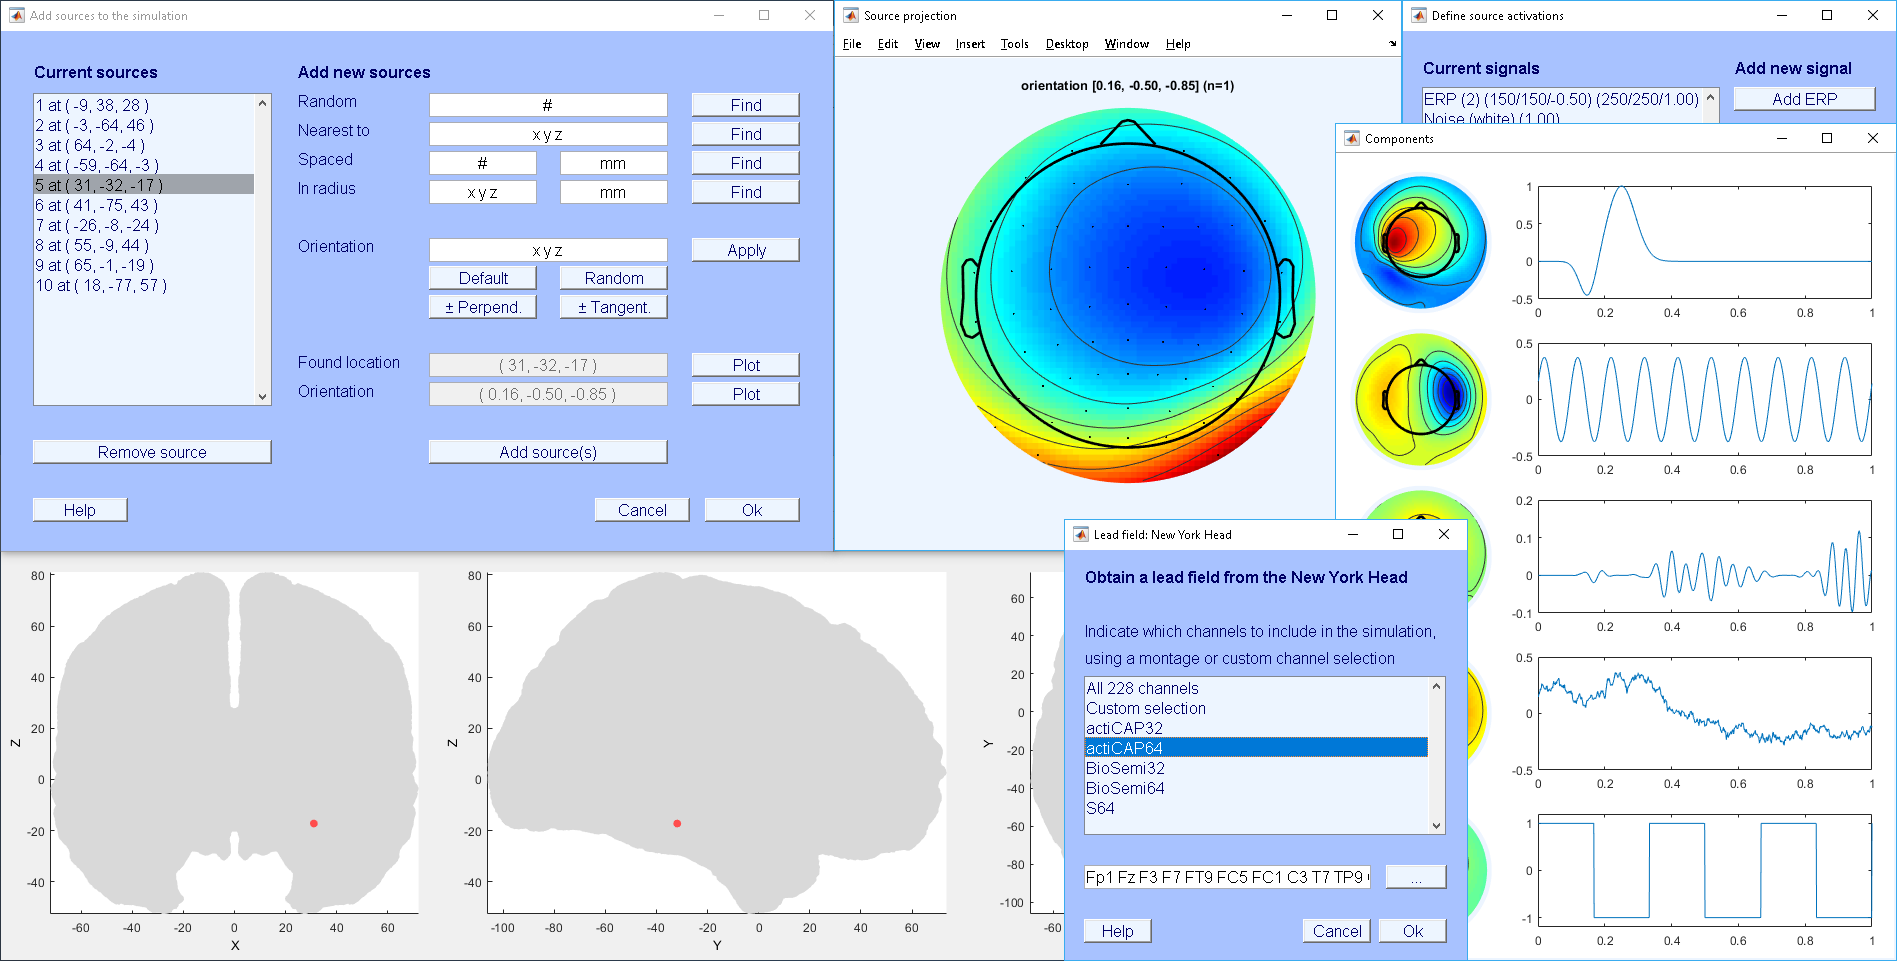
\includegraphics[width=5in]{figures/sereega-gui.png}
    \caption{Impression of the SEREEGA GUI.}
    \label{fig:sereega:gui}
\end{figure}

SEREEGA is available as an EEGLAB plug-in including a graphical user interface (GUI) that allows the core steps of designing and running a simulation to be performed; see figure~\ref{fig:sereega:gui}. For more advanced use, SEREEGA is based on written commands and assignments.

A general configuration variable holds information about the number of epochs to simulate, their length, and their sampling rate. This configuration, as well as many other variables, are contained within MATLAB structure arrays.

SEREEGA's forward model is contained in a \emph{lead field} structure array. The lead field structure contains all possible sources within a virtual brain, modelled as dipoles at specific locations along with their projection patterns. The word \emph{source} thus corresponds to an index in this lead field. For each such index, the lead field contains a position (x, y, z), and projection patterns along three axes (x, y, z). As mentioned in Section~\ref{sereega:principles}, a linear combination of the three projection patterns can effectively be used to virtually define the source dipole's \emph{orientation} in 3D space. A source together with its orientation can be saved as a \emph{component} structure array, which additionally needs to be assigned a \emph{signal}: the simulated neuro-electrical activity that will be projected from it, such as an event-related potential or an oscillation at a specific frequency. These are defined separately and added to the components.

The main workflow consists of defining any number of such components, each containing at least one source, orientation, and signal. The simulation of scalp data finally generates each component's signals and projects them onto the scalp.

The following sections go through the main steps in more detail. Note that these steps must not necessarily be followed in this order.


\subsubsection{Lead Field Generation}

The lead field determines both the maximum possible number of sources as well as the number of channels that will be simulated. Currently, SEREEGA supports two processes to obtain a lead field: it can be obtained from an existing, pre-generated lead field, or a custom lead field can be generated from a given head model. Currently, support for four pre-generated lead fields is included.

\begin{figure}
    \centering
    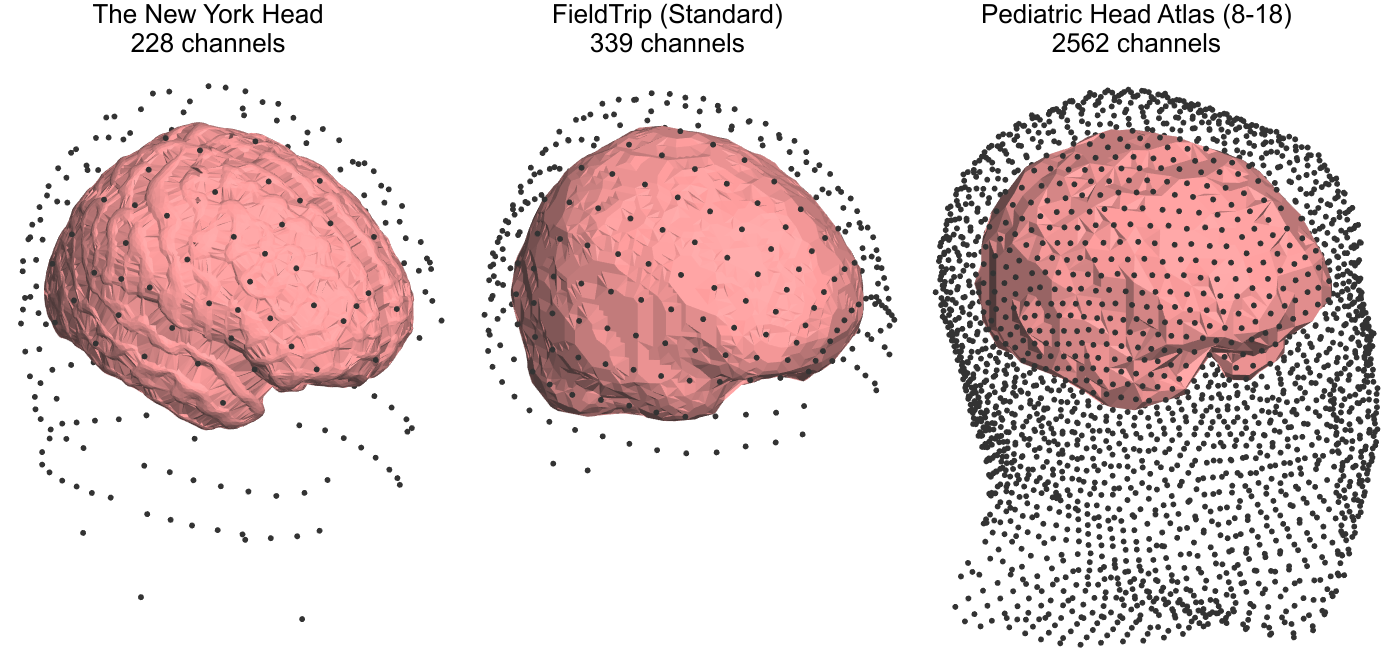
\includegraphics[width=5in]{figures/sereega-headmodels.png}
    \caption[Channel locations and estimated brain boundaries for three head models.]{Channel locations and estimated brain boundaries for three head models. Left: The New York Head with its 228 channels. Middle: a 339-channel layout around a standard average head model available by default in FieldTrip. Right: The Pediatric Head Atlas (8 to 18, version 2) showing 2562 channels.}
    \label{fig:sereega:chanlocs}
\end{figure}

The New York Head (ICBM-NY) pre-generated lead field includes almost 75~000 source locations and their projections onto to 228 channels \cite{huang2016nyhead}. The electrode positions follow the international 10--05 system \cite{oostenveld2001fivepercent} but also include two rows of channels below the ears. Each source comes with a default orientation that orients it perpendicular to the cortical surface. 

The Pediatric Head Atlases comprise three different head models with pre-generated lead fields for up to three different electrode layouts each, ranging from 128 to more than 2500 electrodes \cite{song2013phm}. The models cover heads from three pediatric age clusters, 0--2, 4--8, and 8--18 years old. Lead field sources are spaced in an approximately $1\times1\times1$~mm grid and range from 3188 to 4837 in number. These lead fields do not contain default dipole orientations. For inclusion in SEREEGA, the given electrode and dipole coordinates are transformed upon initialisation to be centred around $(0,0,0)$ and aligned to the axes.

FieldTrip \cite{oostenveld2011fieldtrip} can be used to generate a lead field as needed. Using a given head volume, it can generate any number of sources with a given resolution, projecting to any number of channels. By default, a standard head model and a 339-channel definition file following the international 10--05 system are included. FieldTrip does not provide default source orientations.

When obtaining a lead field, it is possible to only use a subset of the available channels by indicating their labels. Convenience functions are available to simulate standard EEG cap layouts with e.g. 64 channels. Figure~\ref{fig:sereega:chanlocs} shows the available channel locations for three head models.


\subsubsection{Source Selection and Orientation}

The lead field structure contains all possible sources. From these, one or more sources can be selected using different methods to be included in the simulation. It is possible to simply obtain a random source, or to obtain multiple random sources that are at least a given distance apart from each other. It is also possible to select the source nearest to a specific location in the brain, or all sources within a certain radius from a specific location or another source. Sources are referenced using their index in the lead field. Figure~\ref{fig:sereega:source}, left, shows the location of one source using EEGLAB's standard head model and corresponding plotting function. (In this case, EEGLAB's standard head model fits the lead field's head model. SEREEGA's default plotting functions do not depend on this being the case.)

Sources represent dipoles at the indicated location. Having selected a source location, this dipole can be oriented to face different directions, which determines how it projects onto the scalp. The lead field makes this possible by containing the dipole's projection pattern onto all selected electrodes into three mutually perpendicular directions x, y, and z---the base vectors mentioned in Section~\ref{sereega:principles}. A linear combination of these three projection patterns can then be used to effectively orient the dipole in space. Thus, a dipole's orientation is indicated using three values, with $(1,0,0)$ representing a perfect x-positive orientation, $(0, 1, 0)$ y-positive, $(\frac{1}{\sqrt{2}},\frac{1}{\sqrt{2}},0)$ a 45-degree angle with the same amplitude, et cetera. Figure~\ref{fig:sereega:source}, right, shows the three separate patterns as well as a combined projection pattern for one source. 

\begin{figure}
    \centering
    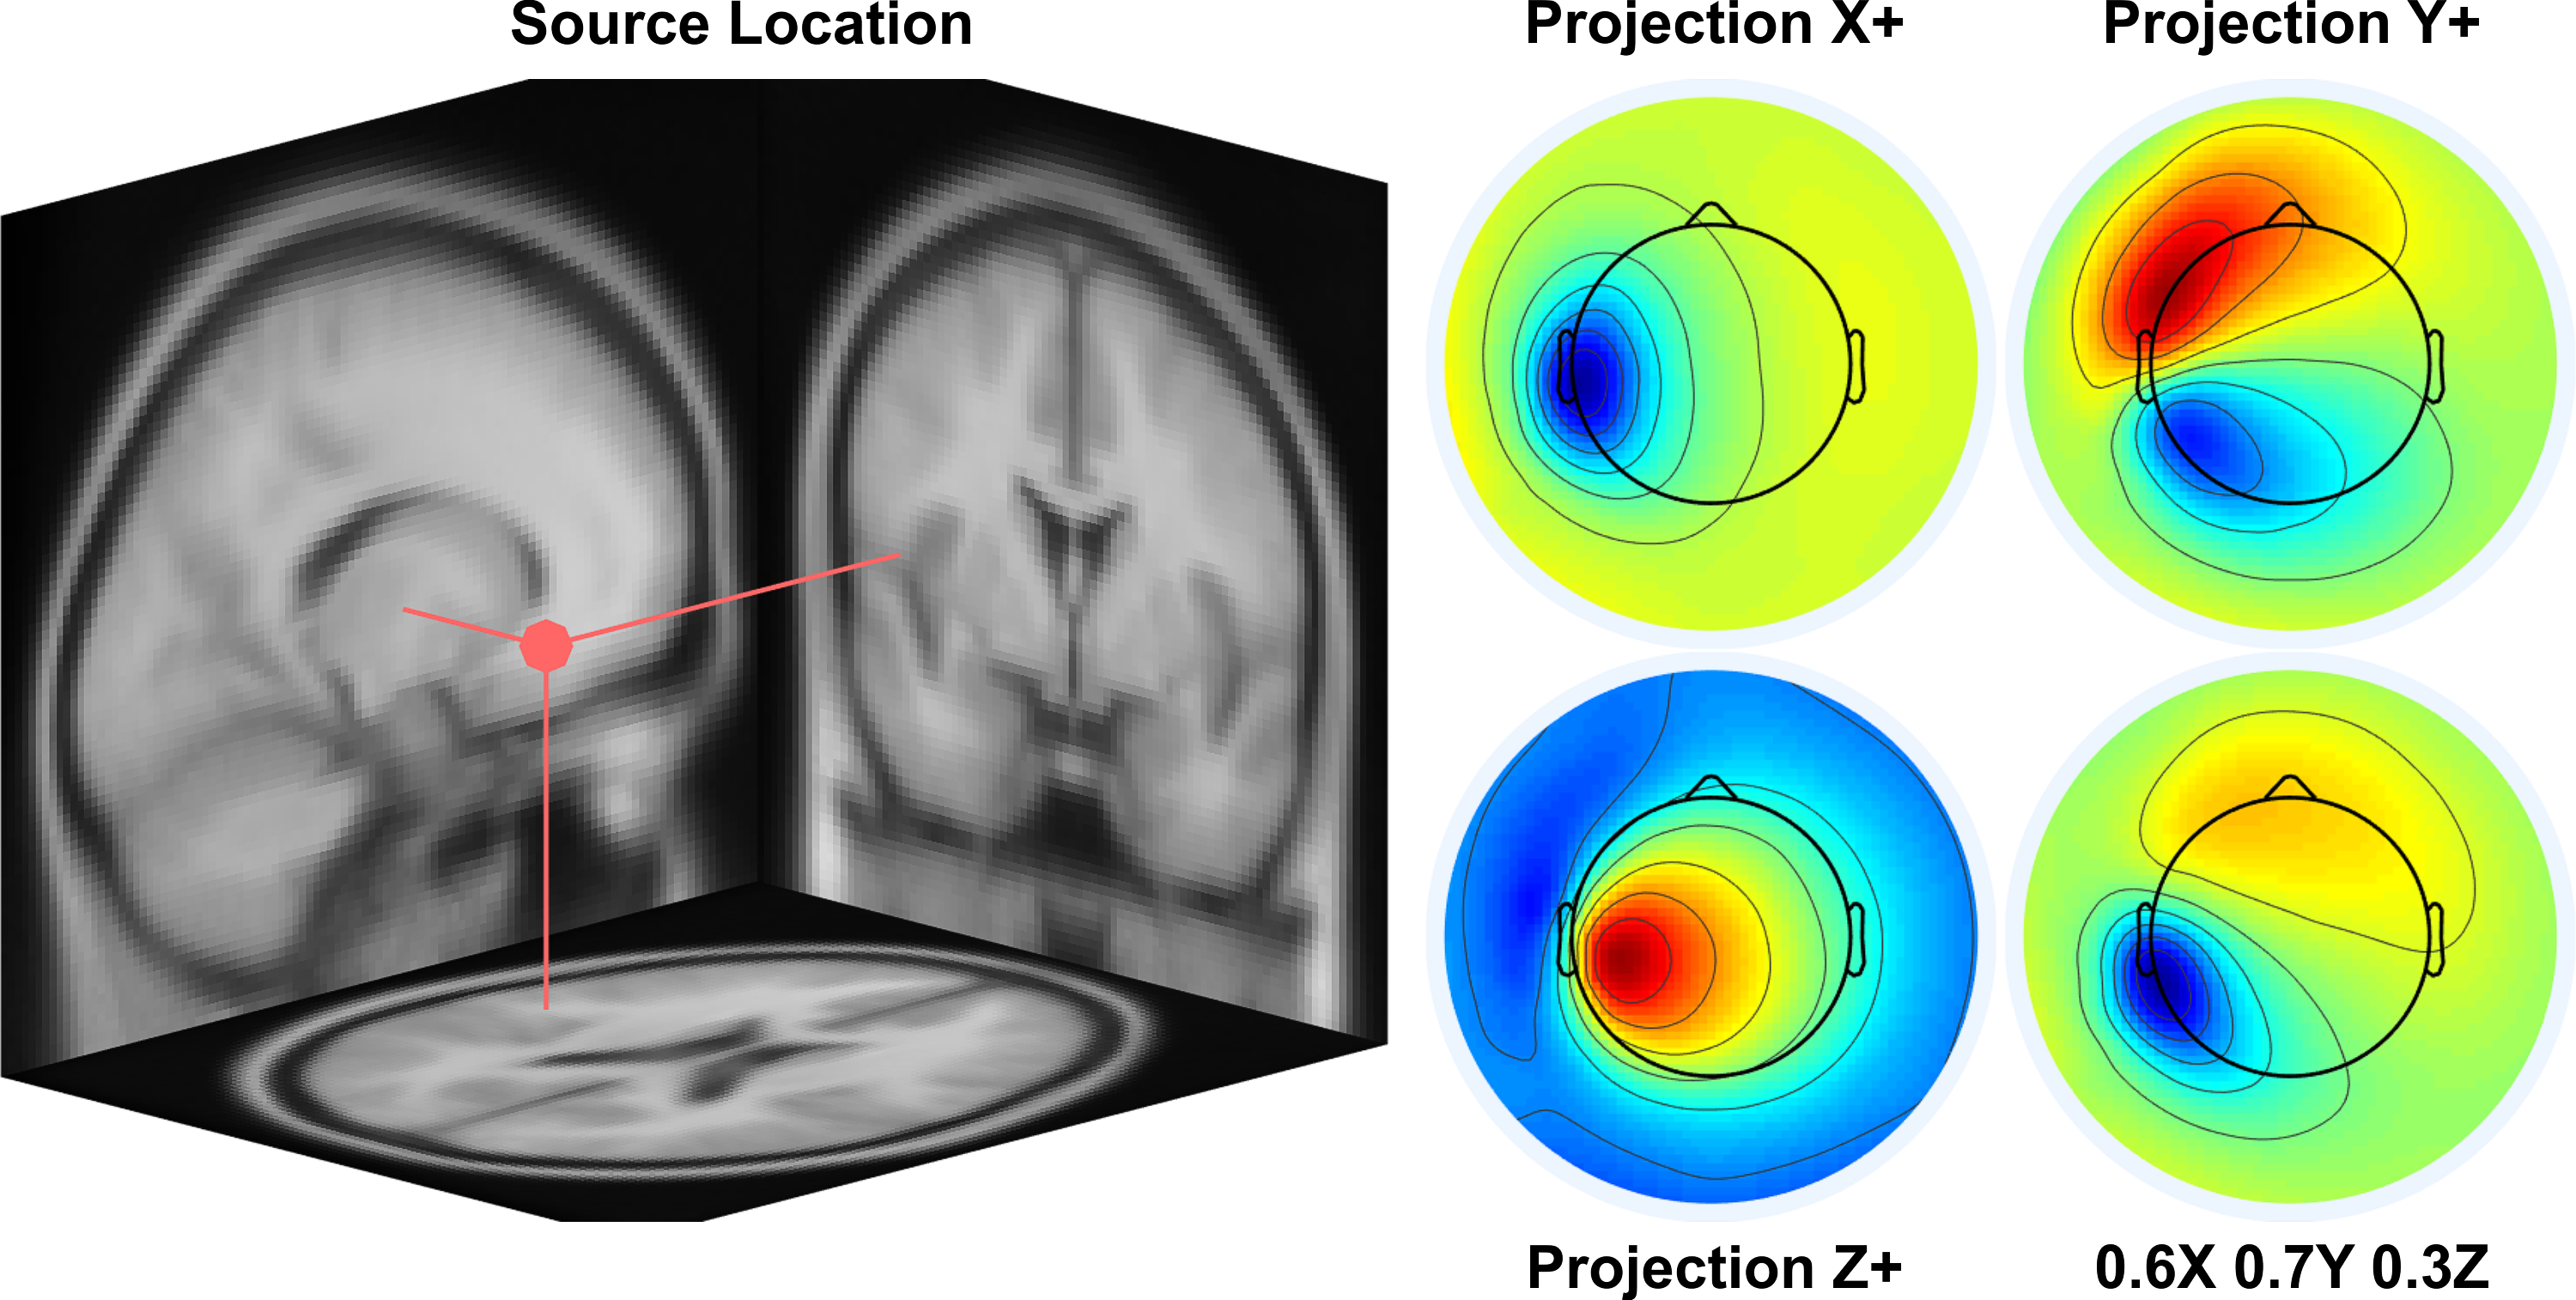
\includegraphics[width=5in]{figures/sereega-source.png}
    \caption[A source dipole's location and projection patterns.]{Left: The location of source number 7479 in the New York Head as plotted onto EEGLAB's standard head model. Right: Four projection patterns of that source onto the scalp. From top left to bottom right: projection in the x-positive, y-positive, and z-positive direction, and a linear combination of the three (arbitrary units). This effectively orients the dipole at the source's location in 3D space.}
    \label{fig:sereega:source}
\end{figure}


\subsubsection{Signal Definition}
\label{sereega:signals}

Having selected a source location and orientation, i.e. a projection pattern, one or more \emph{signals} can be defined to be projected onto the scalp as if they originate from that location. These are defined using \emph{classes}. A class contains a signal's type and any parameters corresponding to that type in a structure array. For each simulated epoch, a signal will be procedurally generated using the parameters of that class.

SEREEGA currently includes four types of signals: systematic deflections in the time domain (i.e., event-related potentials), systematic modulations of oscillatory activity (i.e., event-related spectral perturbations), stochastic processes in the time domain (i.e., noise), and autoregressive signals (i.e., spatio-temporal signals with systematic interactions between them). Figure~\ref{fig:sereega:signals} provides an overview of three of these and their main parameters. A final \emph{data} type enables the inclusion of any already existing time series as an activation signal. The following sections mention the primary free parameters for each type.

\paragraph{Event-Related Potentials} An \emph{event-related potential} \cite<ERP;>{luck2014erp} class defines one or more positive and/or negative `peaks' or deviations from a baseline in sequence. Each peak is determined by its latency in ms, its width in ms, and its amplitude in \si{\micro\volt}. For example, the ERP in figure~\ref{fig:sereega:signals} is a single positive peak at 500~ms, 200~ms wide, of 1~\si{\micro\volt}.

A peak is generated by centring a normal probability density function around the indicated latency with the given width covering 6 standard deviations. This is then scaled to the indicated amplitude. For multiple peaks, each peak is generated individually and then summed together.

\paragraph{Event-Related Spectral Perturbations} Where ERPs represent systematic activity in the time domain, \emph{event-related spectral perturbation} (ERSP) classes are defined primarily using spectral features. The term ERSP refers to event-related spectral power changes \cite{makeig2004eventdynamics}; in SEREEGA, it refers to the class of signals that generate specific spectral powers and/or changes therein.

First, a base frequency is defined, either as a pure sine wave of a single frequency, or as a frequency band. In this latter case, uniform white noise is band-pass filtered in the indicated band using a window-based finite impulse response filter with a Kaiser window and an automatically decided filter order \cite{oppenheim2010dsp}. The left middle panel of figure~\ref{fig:sereega:signals} shows an oscillation of 10~Hz, the panel to the right of that shows filtered noise with power focused between 5 and 10~Hz.

The minimal definition of an ERSP class consists of a frequency (or frequency band) and its amplitude. In case of a single frequency, a phase can optionally be indicated as well. 

In other cases, these parameters merely define a base oscillation that is further modulated. The lower row of figure~\ref{fig:sereega:signals} presents two types of modulations that can be defined for ERSP classes: (inverse) burst modulation and amplitude modulation. The former attenuates or amplifies the signal to a given degree using a Tukey window of given width, latency, and tapering. A Tukey window can be adjusted ranging from a square to a cosine shape. This mimics event-related synchronisation and desynchronisation. The latter modulates the amplitude of the base signal to a given degree according to the phase of a sine wave, whose frequency and phase can be defined in the class. Additionally, a pre-stimulus period can be indicated such that the modulation only starts at a given latency.

\paragraph{Noise} A class of a \emph{noise} signal simply produces coloured noise, from either a normal Gaussian or a uniform distribution, of a given amplitude. A noise class is defined by at least a colour and an amplitude. The upper right panel of figure~\ref{fig:sereega:signals} shows white noise with an amplitude 1 \si{\micro\volt}.

The Gaussian function uses MATLAB's DSP toolbox to generate noise with a spectral characteristic of $1/f^n$, with $n$ either -2, -1, 0, 1, or 2. The uniform function first samples the signal from a uniform distribution and then applies a Fourier transformation to achieve the same spectral characteristic.

\paragraph{Data} For the inclusion of any given pre-existing time series, for example data generated elsewhere or taken from existing EEG recordings, a \emph{data} class can be defined. It must be given a matrix of data, epoch-dependent indices, and an absolute or relative amplitude. It will project the indicated data scaled to the given amplitude for each simulated epoch. 

\paragraph{Autoregressive model} A final type of class generates signals based on a linear \emph{autoregressive model} (ARM), following the approach by \citeA{haufe2016connectivitysimulation}. For a single source activation, this generates a time series where each sample depends linearly on its preceding samples plus a stochastic term. At least the order of the model, i.e. the number of non-zero weights on the preceding samples, and the signal amplitude must be configured. The exact weights of the model are determined automatically.

It is also possible to simulate connectivity between multiple sources. Uni- and bidirectional interactions can be indicated such that a time-delayed influence of one source on another is included in the signal. Either the number of interactions is configured and the toolbox will randomly select the interactions, or a manual configuration of the exact directionalities can be indicated. The model order is the same for all interactions.

Interacting signals are not simulated at runtime, but generated beforehand and included in the simulation as data classes.

\begin{figure}
    \centering
    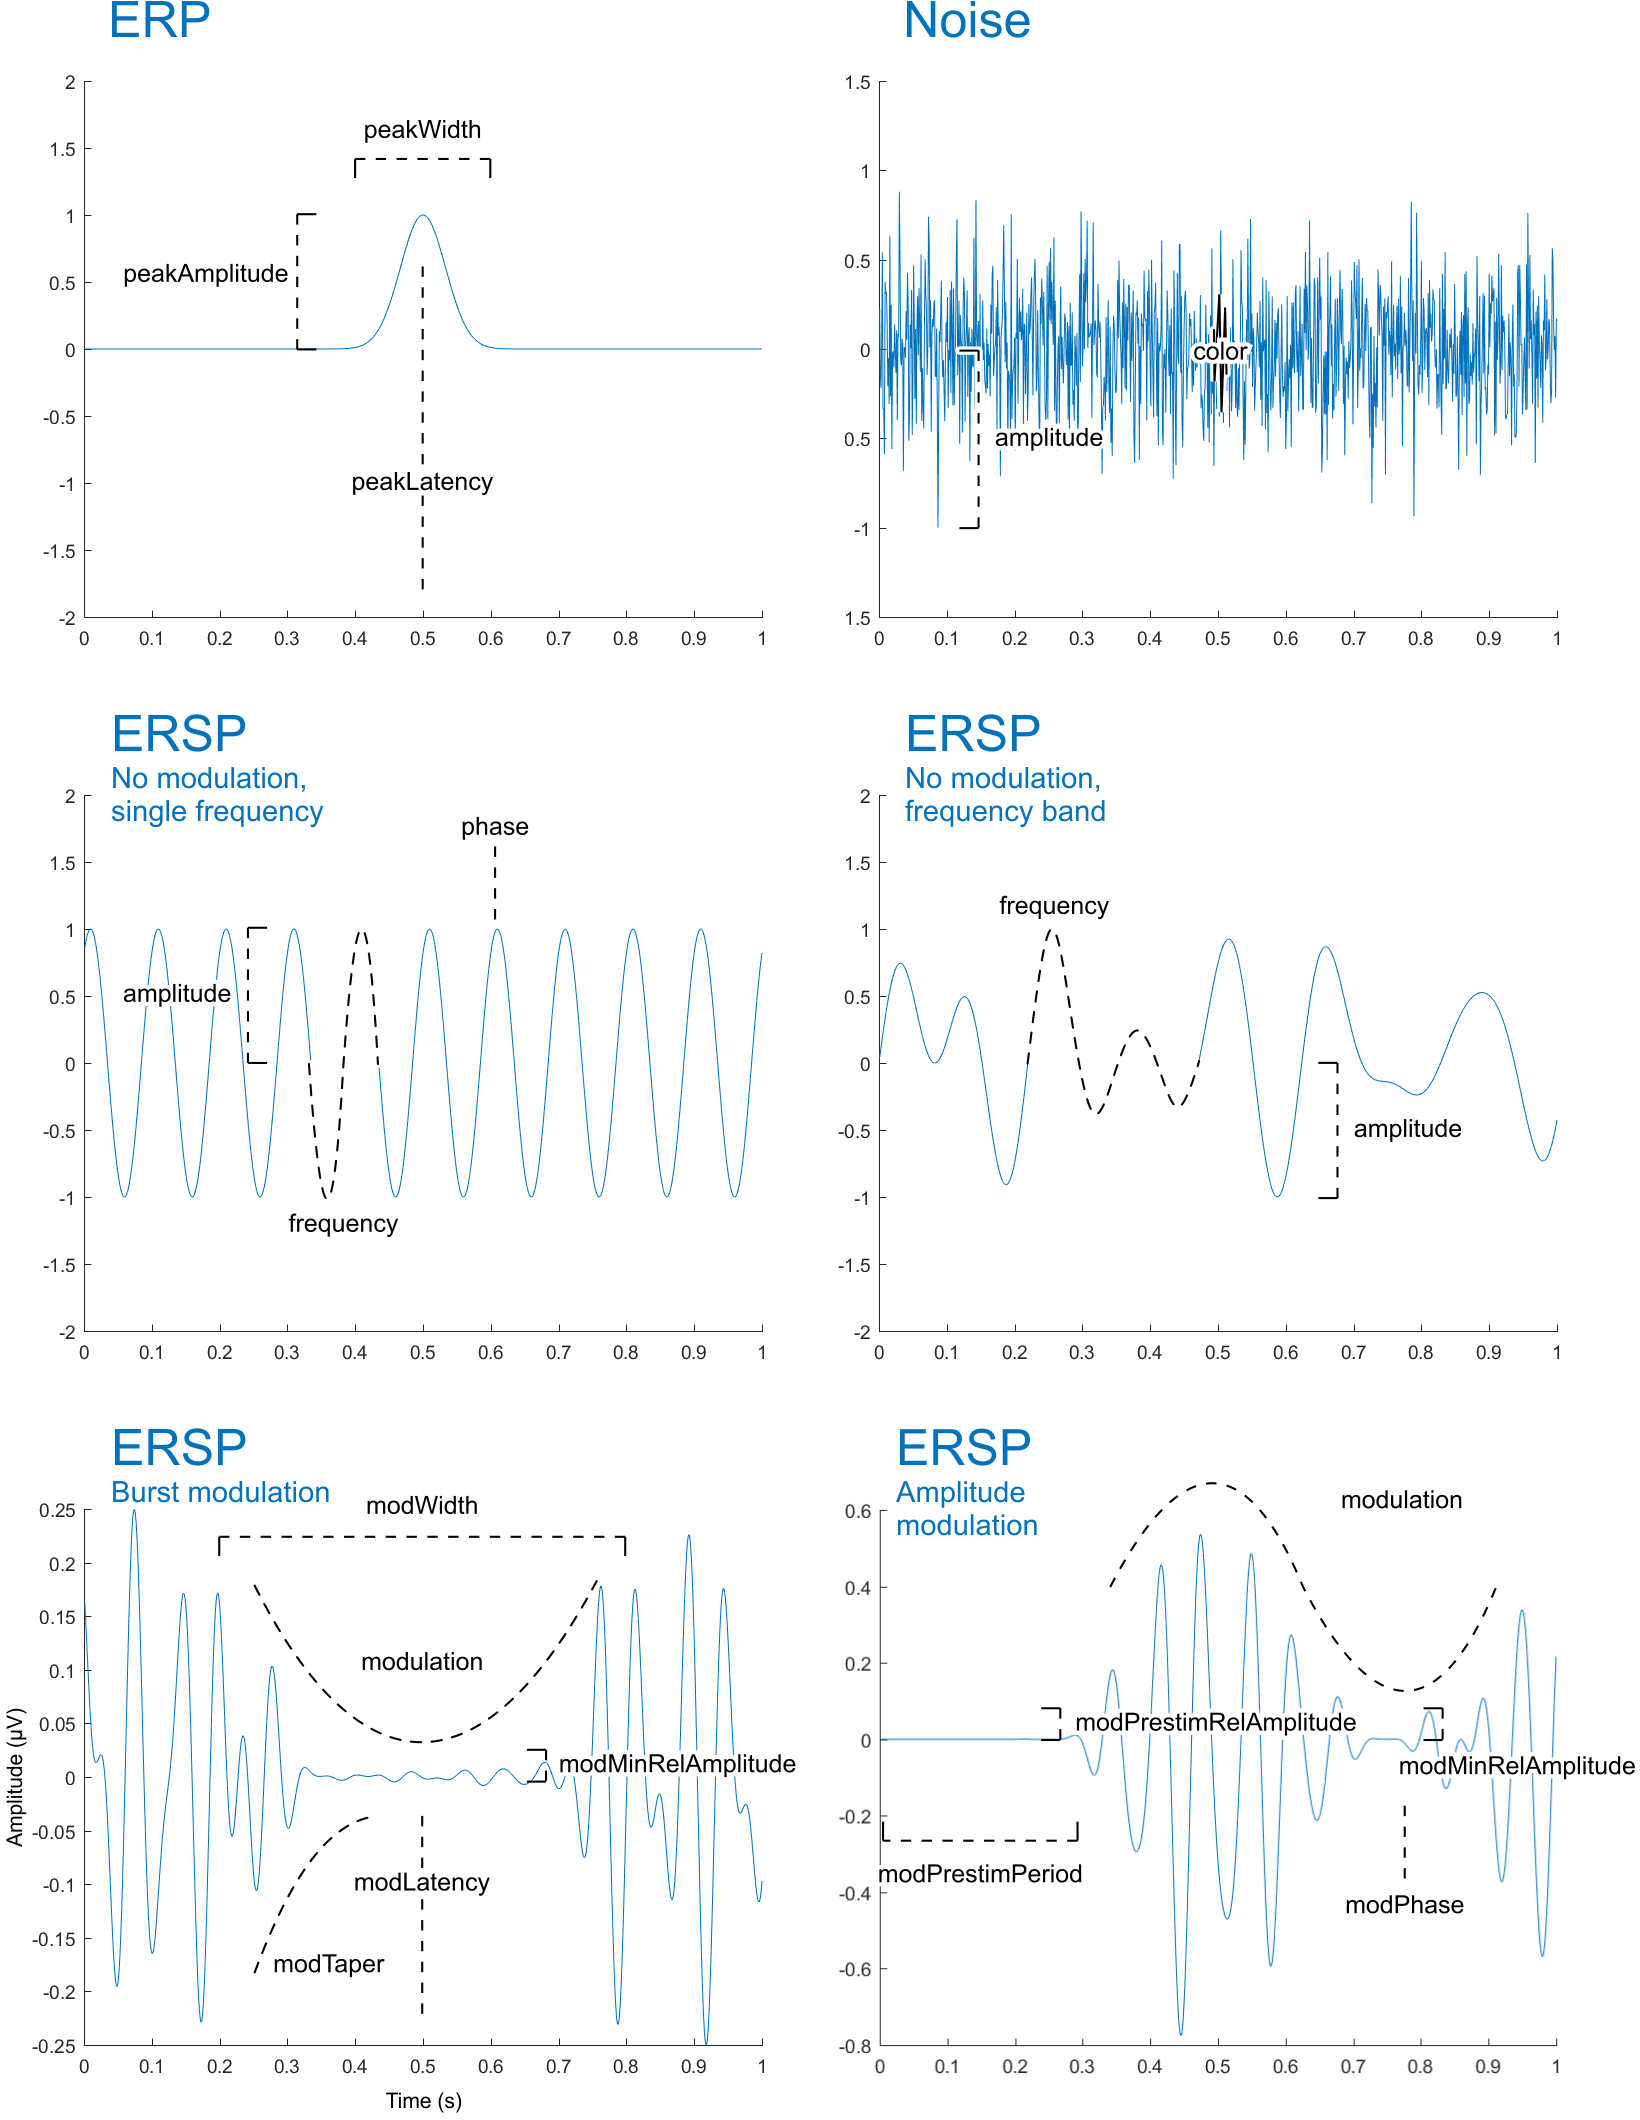
\includegraphics[width=\textwidth]{figures/sereega-signals3x2.png}
    \caption[Sample signals annotated with the base variables that control their behaviour.]{Sample signals annotated with the base variables that control their behaviour. From top left to bottom right: event-related potential (ERP);  coloured noise; single-frequency unmodulated event-related spectral perturbation (ERSP); frequency band unmodulated ERSP; inverse burst-modulated ERSP; amplitude-modulated ERSP. Each base variable can additionally be given a deviation and a slope to control the epoch-to-epoch and systematic progressive variability of the signal. Not illustrated: the autoregressive model (ARM) and data classes.}
    \label{fig:sereega:signals}
\end{figure}


\subsubsection{Variability}

It defeats the purpose of simulating multiple epochs if every epoch were to be exactly the same. To take an ERP as example, it may not be desirable to have a peak defined at 500~ms appear at exactly 500~ms in every epoch. In fact, perhaps the ERP should sometimes not appear at all. To that end, both classes and components contain parameters to add variability to the generated signal.

For all parameters displayed in figure~\ref{fig:sereega:signals} controlling the shape of the various signals, two more parameters exist that control those base parameters: each parameter has a corresponding \emph{deviation} parameter, and a \emph{slope} parameter.

The deviation indicates a range of allowed values. A base value of 2 with a deviation of 0.3, for example, will vary from epoch to epoch between 1.7 ($2-0.3$) and 2.3 ($2+0.3$) following a Gaussian function. Specifically, the range of deviation covers 6 standard deviations. This can be used to model general Gaussian variability within the system. A deviation is calculated for each parameter value separately for each epoch. For some parameters, one additional \emph{shift} parameter is available to make these values deviate with equal magnitude within one epoch. This can be useful to e.g. have the latency of multiple peaks in an ERP vary together, maintaining the overall shape of the ERP.

The slope indicates a systematic change over time. A base value of 2 with a slope of $-0.3$, and no deviation, will be 2 on the first epoch, and 1.7 ($2-0.3$) on the final epoch. In between, it will scale linearly with the number of the current epoch. Slopes can be used to model e.g. effects of fatigue and habituation, or to cover a range of intended values.

Each class also has a \emph{probability} parameter that determines, for each epoch, that signal's probability of appearance. A probability of 0.5 indicates a 50\% chance of the defined signal being generated for any simulated epoch. In case it is not generated, a flatline is returned instead, meaning it does not interfere with any other activations at that time.

Deviation and slope parameters are also available for components, to control the dipole orientation. Components can have one additional source of variability, with respect to the source location itself. Instead of one source index, multiple source indices can be indicated as that component's source. In that case, one of them will be randomly picked for each epoch. As such, together with the orientation variability, spatial variability can be added as well.


\subsubsection{Simulating Scalp EEG}

A \emph{component} is a structure array that contains, for each element, at least one source index, a corresponding orientation, and at least one signal. Thus, by combining the results of the previous two steps into components, it is specified which of the defined signals are projected from which source at which orientation. It is possible to assign more than one signal to a component. To add noise to an ERP, for example, both an ERP and a noise class can be added to the same component. All signals assigned to a component are summed together before being projected. When the same signal class is given to multiple components, a new instance of that signal will be generated for each component at runtime.

There is no limit to the number of components that can be defined, nor to the number of signal classes that can be added to each component.

A simulation function takes the defined components, the lead field, and the general configuration as input, and outputs the simulated scalp data in a $channels \times samples \times epochs$ matrix, as well as $components \times samples \times epochs$ source data. For each epoch, this function follows the forward model described in Section~\ref{sereega:principles} to produce the scalp data. That is, it generates and sums each component's signals, projects them onto the scalp using the given lead field, source location, and orientation, and then sums all the projected activations. Each signal is generated independently of the others. For interacting signals, as with ARM classes, the signals are generated beforehand and included as data classes.

At this stage, a final layer of noise can optionally be added to the simulated scalp data to simulate sensor noise. This is uniform, temporally and spatially uncorrelated white noise.


\subsubsection{Manual and Random Definition of Signal Classes}

As a final point it is worth mentioning that not all of the available parameters must necessarily be set by the user. Only a small number are required, and a validation function automatically sets all others to their default values. All deviation-related values default to zero. Non-zero default values are chosen to be most useful; the phase of an oscillation, for example, defaults to a new random value for each epoch. A convenience function exists to add deviations and/or slopes of a certain percentage of each base value to signal classes. When the lead field contains default source orientations, these will be used automatically when no other orientation has been explicitly indicated.

When multiple components are to be simulated, it is also not necessary to manually define all signals. For one, the same signal can be added to multiple components. Also, convenience functions exist to generate any number of `random' ERP or ERSP classes, based on a range of allowed base values.


\subsubsection{Sample Code}

The following lines of code reflect the workflow explained above, generating 100, 1-second epochs of brown noise from 64 sources spaced at least 25 mm apart, projected onto 64 channels.

{\footnotesize
\begin{verbatim}
epochs     = struct('n', 100, 'length', 1000, 'srate', 1000);
leadfield  = lf_generate_fromnyhead('montage', 'S64');
sourcelocs = lf_get_source_spaced(leadfield, 64, 25);
signal     = struct('type', 'noise', 'color', 'brown', ...
                    'amplitude', 1, 'amplitudeDv', .5);
components = utl_create_component(sourcelocs, signal, leadfield);
data       = generate_scalpdata(components, leadfield, epochs);
EEG        = utl_create_eeglabdataset(data, epochs, leadfield);
EEG        = utl_add_icaweights_toeeglabdataset(EEG, components, leadfield);
\end{verbatim}
}

The \texttt{epochs} structure array contains three fields configuring the number of epochs, their length in ms, and the sampling rate in Hz. On the next line, a lead field is obtained from the New York Head using a preconfigured montage of 64 channels. Next, 64 source locations are randomly selected from the lead field, such that each source is at least 25~mm apart from all the others. As a signal, brown noise is used with an amplitude varying between 0.5 and 1.5 for each epoch. 64 components are then created by combining that same signal with the 64 previously-defined source locations. Because the New York Head is used, no orientations must be indicated explicitly: the toolbox will use the default values included in the lead field. Finally, scalp data is generated: \texttt{generate\_scalpdata} simulates the components' signals, projects them according to their respective orientations through the lead field, and generates the data set as configured in \texttt{epochs}. In the last two lines of code, the data set is transformed into an EEGLAB-compatible format, and a ground-truth ICA decomposition is added. 

When using the GUI, these steps would be followed in more or less the same order.


\section{Sample Data Set}

To demonstrate some of the toolbox's basic functionality, we now present a sample data set that was generated using SEREEGA and simulates a number of known cortical effects during a hypothetical experiment. We then apply established analysis methods to this data and present the results.


\subsection{Simulated Experiment and Cortical Effects}

The hypothetical experiment represents a visual go/no-go experiment. The visual stimulus in question is a pattern change, eliciting a N70-P100-N135 complex over occipital sites \cite{pratt2011sensoryerp}. In the `go' condition, the pattern change represents a target stimulus eliciting a strong P3a-P3b complex, most pronounced over the parietal-central-frontal midline \cite{polich2007p300}. Upon perception of the target stimulus, the participants initiate a manual response with their right hand, resulting in mu- and beta band desynchronisation over sites covering the contralateral motor cortex.

Specifically, the visually evoked potential complex was modelled after findings by \citeA{gomezgonzalez1994} and \citeA{pratt2011sensoryerp}. The N70 was a single dipole projecting centrally from the visual cortex. The P100 and N135 projected bilaterally from Brodmann areas BA~17 and BA~18, respectively. The P3a-P3b was modelled after \citeA{polich2007p300} and \citeA{debener2005oddballp3} with dipole locations taken from the latter. The manual response, finally, mimics mu- and beta-band findings of manually responded visual targets by \citeA{makeig2004visualmanual}.

The visually evoked potentials were modelled as single-peak ERP classes centred around 70, 100, and 135~ms, respectively, with widths of 60, 60, and 100~ms, and amplitudes of 7.5, 7.5, and 10~\si{\micro\volt}, as well as amplitude slopes of -2, -2, and -3 to simulate a level of habituation \cite{pratt2011sensoryerp}.

The P3a is an ERP class with a single 400~ms wide peak at 300~ms of amplitude 10~\si{\micro\volt}, and an amplitude slope of -5, simulating fatigue \cite{polich2007p300}. The P3b ERP consists of two peaks. One at 400~ms (width 600~ms, amplitude 7~\si{\micro\volt}, amplitude slope -5), and one at 500~ms (width 1000~ms, amplitude 2~\si{\micro\volt}, amplitude slope -1). This latter peak represents the longer-lasting effects of the P3. The stronger slope of the P3b as compared to the P3a is a known finding reflecting habituation to the stimulus \cite{polich2007p300}. All parameters of the ERP classes were given a deviation of 20\% of their value relative to stimulus onset.

The motor cortex is simulated using four components for each class: both left and right motor cortex components are included, each with mu and beta band effects. In the non-target condition all components simply emit resting state mu (here as 8--12~Hz) and beta (19--26~Hz) activity implemented using the ERSP class with no modulation, and an amplitude of 2~\si{\micro\volt}. In the target condition, the left motor cortex classes are given an inverse burst modulation centred around 650~ms (mu; width 600~ms, taper .5, relative amplitude .5) and 600~ms (beta; width 500~ms, taper .8, relative amplitude .5) respectively. ERSP parameters had a deviation of 10\% relative to stimulus onset, with the exception of latency deviation, which was fixed at 100~ms.

To simulate background processes, brown noise was added to each component (as per \citeNP{freeman2009}), with an amplitude of 5~\si{\micro\volt}. Furthermore, brown noise was also projected from a random selection of source locations, such that the total number of components in the data set was 64, all at least 25~mm apart from each other.

A single `base' participant was defined and simulated using the specified component locations and orientations. For 10 subsequent participants, each component's location was randomly chosen within~20 mm of the original locations. Dipole orientations were randomly varied to be within $\pm 25$\% of the original value for each axis. 

This data set was simulated using the New York Head Model and projected onto the S64 montage of 64 channels. For each condition (target versus non-target), 100 epochs were simulated of 2000~ms each with a 500~ms pre-stimulus period, at a sampling rate of 1000~Hz.


\subsection{Analyses and Results}

The generated data set was subjected to a number of standard analyses to demonstrate their applicability and to illustrate the data itself.

First, figure~\ref{fig:sereega:erpimages} shows a single-subject ERP image analysis at three midline electrodes of the `base participant'. This clearly shows the N70-P100-N135 complex, pronounced most strongly at parietal-occipital sites, as well as the P3, with the P3a most prominent over fronto-central sites and the P3b more pronounced further centrally and parietally. Also visible is the epoch-to-epoch variability of the ERP signals in time and in amplitude, as well as their spatial differences with peaks pronounced differently at different sites. The effects over time can also be seen, with amplitudes diminishing at different rates.

\begin{figure}
    \centering
    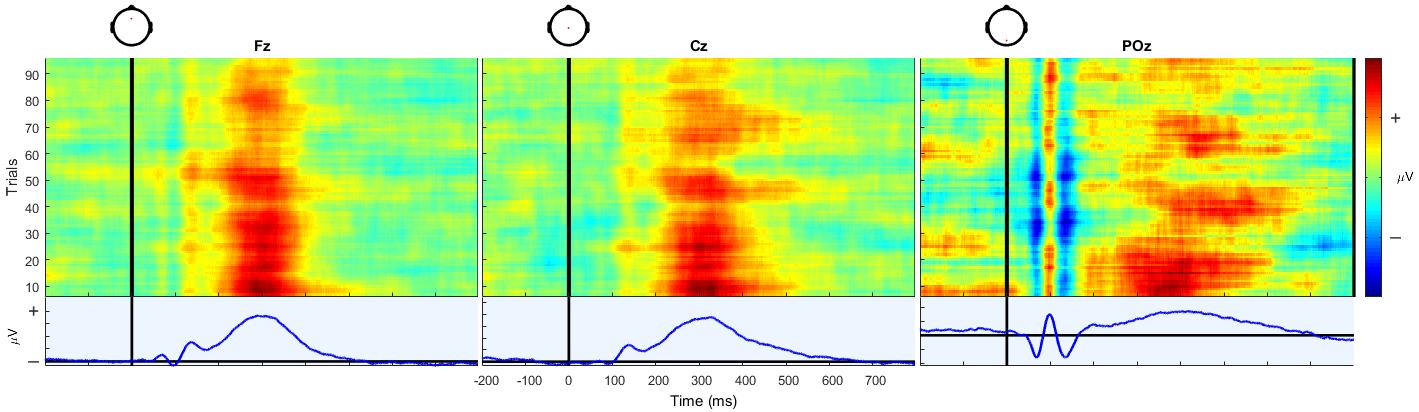
\includegraphics[width=\textwidth]{figures/sereega-erpimages.png}
    \caption[ERP image showing epoch-to-epoch variability as well as spatial differences of simulated data.]{ERP image \protect\cite{makeig2004eventdynamics} at channel Fz, Cz, and POz showing the epoch-to-epoch variability of the simulated ERP signals as well as their spatial differences and effects over time.}
    \label{fig:sereega:erpimages}
\end{figure}

Second, a cluster-based group-level analysis was performed. Using DIPFIT \cite{oostenveld2003dipfit}, equivalent dipole locations were reconstructed from the data set's ICA decomposition. These locations as well as the independent components' calculated ERSPs were used for k-means clustering. Due to the variability of the data as well as the clustering algorithm, manual adjustment was still necessary to create one cluster containing all left motor cortex components. The calculated dipole locations are given in figure~\ref{fig:sereega:cluster}. As was defined, they vary around a given mean location. Figure~\ref{fig:sereega:mcersp} shows the mean calculated event-related spectral perturbation for this cluster for both the target (left) and the non-target (right) conditions. The target condition shows clear mu and beta effects similar to those found by \citeA[figure~8]{makeig2004visualmanual}.

\begin{figure}
    \centering
    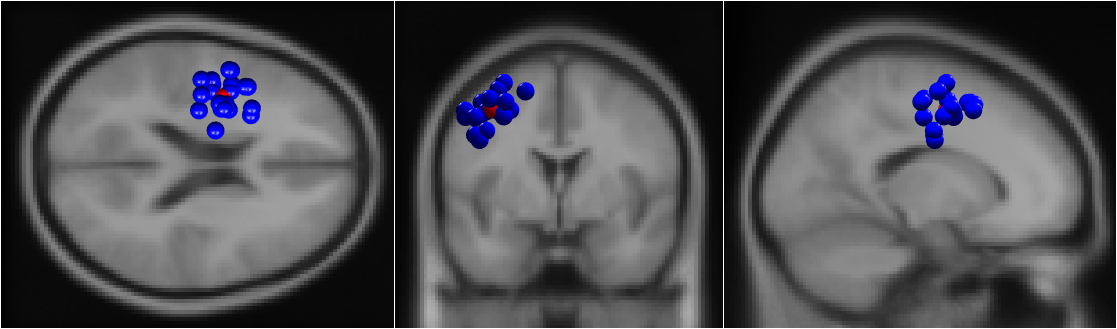
\includegraphics[width=\textwidth]{figures/sereega-cluster.png}
    \caption[Locations of the left motor cortex equivalent dipoles in each simulated participant.]{Locations of the left motor cortex equivalent dipoles in each simulated participant, from DIPFIT \protect\cite{oostenveld2003dipfit} calculations based on the independent components' scalp maps.}
    \label{fig:sereega:cluster}
\end{figure}

\begin{figure}
    \centering
    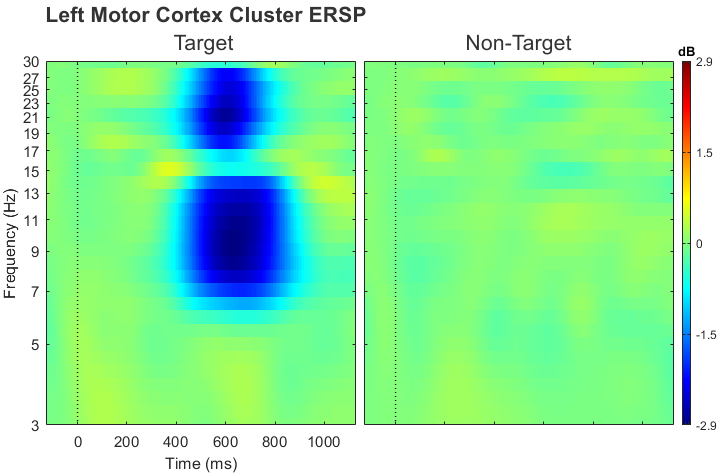
\includegraphics[width=3in]{figures/sereega-mcersp.png}
    \caption[Mean event-related spectral perturbation calculated for the simulated left motor cortex cluster.]{Mean event-related spectral perturbation calculated for the left motor cortex cluster. Left: target condition (right-manual response). Right: non-target condition (no response).}
    \label{fig:sereega:mcersp}
\end{figure}

Finally, the data was subjected to an analysis of classifiability for a hypothetical BCI system to be able to detect the elevated P3 response in the target condition compared to the non-target condition, and, separately, the manual response.

The P3 classifier followed a windowed means approach \cite{blankertz2011}, using the mean amplitude of six consecutive 50~ms time windows starting 200~ms after stimulus onset as features. Before, the signal was bandpass-filtered between 0.1 and 15~Hz. 

The manual response was classified using a logBP approach \cite{pfurtscheller2001motorimagery}, using as features the power between 7 and 27~Hz, 400 to 1000~ms after stimulus onset, focused on sites covering the motor cortex: FC1, FC2, FC3, FC4, FC5, FC6,  C1, C2, C3, C4, C5, and C6.

Both classifiers were implemented using BCILAB \cite{kothe2013bcilab}. A regularised linear discriminant analysis classifier was trained to separate classes \cite{duda2001}. A $5\times5$ nested cross-validation with margins of 5 was used to select the shrinkage regularisation parameter, and to generate the estimates of the classifiers' accuracy listed in table~\ref{tab:sereega:bci}. With chance level at 50\% and significance reached at 57\% \cite{mullerputz2008random}, we see that both classifiers reach significance for all `participants', with the exception of participant 5, where no significant difference could be detected between the elicited P3 responses of the two conditions.

This shows the data's variability on another level and demonstrates that levels of significance can be achieved with neither a ceiling nor a floor effect.

\begin{table}[ht]
    \centering
    \begin{tabular}{lcccccc}
    \hline
    \textbf{Participant} & \textbf{WM TP} & \textbf{WM TN} & \textbf{WM Acc} & \textbf{BP TP} & \textbf{BP TN} & \textbf{BP Acc} \\
    \hline
    0           & 0.78   & 0.75   & 0.76    & 0.70    & 0.64    & 0.67     \\
    1           & 0.76   & 0.69   & 0.72    & 0.67    & 0.69    & 0.68     \\
    2           & 0.74   & 0.74   & 0.74    & 0.57    & 0.58    & 0.57     \\
    3           & 0.77   & 0.72   & 0.74    & 0.61    & 0.62    & 0.61     \\
    4           & 0.72   & 0.57   & 0.64    & 0.65    & 0.64    & 0.64     \\
    5           & 0.55   & 0.58   & 0.56    & 0.66    & 0.69    & 0.67     \\
    6           & 0.68   & 0.57   & 0.62    & 0.61    & 0.70    & 0.65     \\
    7           & 0.71   & 0.64   & 0.67    & 0.70    & 0.68    & 0.69     \\
    8           & 0.71   & 0.61   & 0.66    & 0.63    & 0.55    & 0.59     \\
    9           & 0.76   & 0.67   & 0.71    & 0.56    & 0.59    & 0.57     \\
    10          & 0.67   & 0.57   & 0.62    & 0.69    & 0.64    & 0.66     \\
    \textbf{Mean}        & \textbf{0.72}   & \textbf{0.65}   & \textbf{0.69}    & \textbf{0.64}    & \textbf{0.64}    & \textbf{0.64} \\
    \hline
    \end{tabular}
    \caption[Classification accuracies for windowed-means and band-power classifiers on simulated data.]{Classification accuracies for two classifiers, one using the windowed means approach (WM) and one based on band power (BP). TP = true positive rate, TN = true negative rate, Acc = overall accuracy. Significance is reached at an accuracy of 0.57. The WM classifier for participant 5 does not reach significance.}
    \label{tab:sereega:bci}
\end{table}


\section{Discussion}

In this paper we presented the core functionality of SEREEGA, a free and open-source MATLAB-based toolbox to simulate event-related EEG activity. SEREEGA allows any number of components to be defined in a virtual brain model, each with a specific location in the brain, a freely oriented scalp projection, and any number of signals. Five different types of activity are currently supported, allowing systematic effects in both the time and frequency domain to be simulated, mimicking known EEG features. Simulated EEG data can serve as ground truth for the development of new EEG analysis methods or the validation of existing ones.

The presented data set serves as a demonstration of some of SEREEGA's functions: a set of known cortical effects was simulated, mimicking a hypothetical experiment. It furthermore demonstrates how a basic initial configuration can be procedurally varied to simulate any number of additional participants with different anatomical layouts and variations in their cortical responses, leading to different results for example with respect to classification accuracies. 

The classification accuracies presented here were only around 7 to 12 percentage points above significance on average. This is primarily due to the relative amplitude of the added noise, i.e., the signal-to-noise ratio of the generated data set. This can easily be varied to increase or decrease the classification accuracies as needed, or to investigate the accuracy as a function of this ratio. SEREEGA allows signal and noise components to be simulated separately, and then mixed to achieve a specific signal-to-noise ratio.

The ability to generate data as needed should be met with some caution. When validating signal detection mechanisms, for example, insufficiently considered parameters may lead to trivial results. Similarly, there is a potential danger of making circular arguments. For example, when SEREEGA is used to model a linear effect, and a linear method is subsequently used to again identify this effect, the obtained results could be essentially tautological. In such a case, the results would be applicable only to the extent that real EEG data contains a comparable linear effect. More generally, properties of signal simulation methods are based on assumptions that must not necessarily, or not fully, be met in real EEG data, and this limits the transfer of findings from simulated data to real recordings. This is a fundamental property of all simulation approaches, and users of simulations should be aware of the generator algorithms underlying the data, how they relate to the methods they are investigating, and how they may or may not relate to real EEG recordings.

Indeed, the open architecture of any general-purpose toolbox places some responsibility with the user to make use of the tools in a way that is compatible with the tested hypothesis. Different analysis methods have different assumptions as to e.g. the number of active sources or the statistical properties of the source signals. While SEREEGA is capable of adhering to a large variety of assumptions, not all data that is produced by it will adhere to the same ones. This depends on the design of the data.

It is thus highly important to carefully consider a simulation's parameters. With SEREEGA, different levels of complexity and realism can be generated. For some purposes, there may be no explicit need to simulate complex data sets or otherwise precisely model specific known cortical effects: The results of the methods may hold regardless of the complexity of the simulation. For example, to validate, in theory, a method such as logBP, a pure sine wave among white noise in a low number of randomly mixed channels may suffice. However, other methods do require a higher level of realism with e.g. a higher number of channels and realistic spatial dependencies, a higher number of noise sources, et cetera. For the sake of demonstration, we opted for a more realistic hypothetical experiment to demonstrate in this paper. We do not mean to say however that this level of realism is the explicit goal of SEREEGA, nor that it is methodically preferable. We did intend to illustrates how SEREEGA \emph{can} be used for this purpose. 

It should also be mentioned that realism here refers to the ultimately simulated source and scalp signals, not their underlying neurophysiology. As such, for example, ERPs are simulated directly as ERP-like time series, not as e.g. lower-level phase-resetting oscillations. Similarly, other known EEG effects such as phase-amplitude coupling, travelling waves, EEG microstates, and certain cross-trial dependencies are also not currently implemented. Additional signal classes or component properties would have to be written before testing methods that require such types of signal generators. The online documentation provides a tutorial.

Another important factor in a simulation's level of realism is how realistic the noise is. The included stochastic noise processes follow current simulation standards, where in particular $1/f$ and $1/f^2$ frequency scales have been identified to characterise EEG \cite{bedard2006freqscaling,freeman2009}. This is most likely a simplification. Empirical EEG recordings may have different spectral properties, especially non-stationarities over time, and are influenced by deeper and smaller processes whose activity is not directly measurable using EEG. However, there is currently no consensus regarding an alternative noise simulation method. In SEREEGA, any time series can be included in a simulation using the data class. This also allows noise extracted from empirical EEG recordings to be used. Where available, this may be a better solution. In the future, we may consider a public database of such recordings for all users to draw from. In fact, such a database could contain empirical recordings reflecting known cortical responses as well, allowing simulations to be pieced together by combining different parts of real EEG data. For this to be feasible, a large number of empirical data sets must be made available using a single, standardised format to describe them. Hierarchical Event Descriptor (HED) tags \cite{bigdelyshamlo2016hedtags} offer a way to do that, and the Human Electrophysiology, Anatomic Data and Integrated Tools (HeadIT) Resource is one such database that could serve as precursor to the database needed for this purpose \cite{headit}.

Notable sources of artefacts are the eyes and muscles. The head models currently included in SEREEGA are cortical models and do not contain sources in the eyes or muscles. To the best of the authors' knowledge, no head model is currently available that does. A project is currently underway to construct a head model that contains a larger part of the human anatomy. For the moment, SEREEGA allows custom sources to be added to a simulation, by manually providing their coordinates and projection patterns. These can be taken from empirical recordings.

When taking data from empirical recordings, potential anatomical differences should be taken into account. Since SEREEGA supports different head models, it is not necessarily the case that they use the same coordinate format (e.g. Talairach, MNI, or custom measurements). Sources found at the same $[x,y,z]$ location in different empirical studies or SEREEGA scripts may correspond to different actual locations depending on the head model used. Although authors who publish head models and lead fields often take great care to standardise their formats, they are not all uniform. Sometimes this is necessary: the dimensions of the Pediatric Head Atlas covering zero- to two-year-olds are of course smaller than those of an adult human's head model. SEREEGA includes plotting functions to investigate the size, shape, and location of a lead field's head model and the sources contained within, as well as to compare them against a standard adult head.

To the extent that their details were sufficiently reported, all (software) simulations that were performed by the authors mentioned in the introduction of this paper can be done using SEREEGA. The five signal types and other functions of SEREEGA cover and extend the processes used in those methods. This refers to the core steps of each simulation---further implementation details may of course differ. SIFT, for example, being focused on connectivity, has more options to control the parameters of the autoregressive models than SEREEGA currently does.

A limitation in the current architecture is that the defined components are necessarily independent at runtime: the procedurally generated activity of one component cannot presently depend on the activity in another. For such interactions to be modelled, the signals must be generated beforehand and included as data classes, as is the case for the autoregressive models.

In its current version, SEREEGA makes five accurate, high-density head models accessible in one toolbox, and allows five types of activation signals, enabling coloured noise, ERP-like deflections in the time domain, oscillatory activity with specific spectral characteristics and/or temporal modulations, and autoregressive signals to be simulated, as well as the inclusion of any other pre-generated or pre-recorded time series. This covers and extends the vast majority of past and present-day EEG simulation approaches. Additionally, FieldTrip-generated lead fields based on standard or custom head models can be used, and the toolbox's architecture allows it to be readily extended with additional head models and signals. For more specific needs, SEREEGA has been designed to be modular with extendability in mind.

SEREEGA thus represents, for the first time, an extensive general-purpose toolbox dedicated to simulating event-related EEG activity, making simulation methods more accessible, standardised, and reproducible. 

With SEREEGA, we hope to help developers of EEG-based methods by making data simulation more accessible. With the consistent and increasing popularity of EEG, there is an accompanying need to further develop and validate EEG analysis methods. Simulated data can help with that by providing a ground truth to verify these methods' results. Seeing the current scope of application of simulated EEG studies, we believe that SEREEGA can help with the great majority of these, and can be easily extended for most of the remaining needs. 


\section*{Acknowledgements}

Part of this work was supported by the Deutsche Forschungsgemeinschaft (grant number ZA 821/3-1), Idex Bordeaux and LabEX CPU/SysNum, and the European Research Council with the BrainConquest project (grant number ERC-2016-STG-714567). The authors thank Mahta Mousavi for the band-pass filter design, Stefan Haufe for the autoregressive signal generation code and accompanying support, and Ram\'on Mart\'inez-Cancino for his assistance with the GUI development.


\section*{References}

A shared bibliography starts at page~\pageref{bibliography}.


\clearpage
\pagestyle{plain}

        
\chapter{Towards Classifier Visualisation in 3D Source Space}
\chaptermark{Towards Classifier Visualisation in 3D Source Space}%
\label{chapter:visualisation}%


{\chaptermeta

\textbf{Krol, L. R.\textsuperscript{1}, Mousavi, M.\textsuperscript{2}, de Sa, V. R.\textsuperscript{3}, \& Zander, T. O.\textsuperscript{4}}

{\small
\textsuperscript{1}Biological Psychology and Neuroergonomics, Technische Universität Berlin, Berlin, Germany
\textsuperscript{2}Electrical and Computer Engineering, University of California San Diego, San Diego, USA
\textsuperscript{3}Cognitive Science, University of California San Diego, San Diego, USA
\textsuperscript{4}Zander Laboratories B.V., Amsterdam, the Netherlands

This is the postprint version of the manuscript published as follows:

Krol, L. R., Mousavi, M., de Sa, V. R., \& Zander, T. O. (2018). Towards Classifier Visualisation in 3D Source Space. In \emph{2018 IEEE International Conference on Systems, Man and Cybernetics (SMC)} (pp. 71–76). doi: 10.1109/SMC.2018.00022\nocite{krol2018classvis}

© 2018 IEEE. Reprinted, with permission, from Krol, L. R., Mousavi, M., de Sa, V. R., \& Zander, T. O., Towards Classifier Visualisation in 3D Source Space, October 2018.
\par}}


\abstract%
In the context of brain-computer interfacing, it is important to investigate what regions of the brain a classifier focuses on. For one, this will clarify to what extent the classifier relies on brain activity, as opposed to undesirable non-cortical signals. More generally, the practice is informative as it allows conclusions to be drawn about the cortical regions---and thus, cortical functions---that contribute to the effect under investigation. In this study, we start to investigate different methods to visualise the regions of interest of classifiers based on windowed means and on common spatial patterns. Specifically, we take individually reconstructed source spaces and transform the classifier filter weights into relevance weights indicating the relative contribution of each source to the classifier. This is visualised across participants in an average brain. By decomposing the classifier weights into separate sources and localising these in the brain, this method provides a tool to evaluate classifiers and test hypotheses.


\clearpage


\fancypagestyle{visualisation}{%
    \fancyhf{}
    \fancyhead[EC]{\textit{\leftmark}}
    \fancyhead[OC]{\textit{\rightmark}}
    \fancyfoot[C]{\thepage \\ \vspace{6.8mm} \colorbox{footerbg}{\parbox{\paperwidth-2\fboxsep}{\centering\parbox{0.75\paperwidth}{\centering\fontsize{9pt}{9pt}\selectfont\textcolor{footerfg}{This is the postprint version of published manuscript: Krol, L. R., Mousavi, M., de Sa, V. R., \& Zander, T. O. (2018). \\ Towards Classifier Visualisation in 3D Source Space. In \textit{2018 IEEE International Conference on Systems, Man and Cybernetics (SMC)} (pp. 71–76). © 2018 IEEE.}}}}}
    \fancyfootoffset[]{1.25in}}
\pagestyle{visualisation}


\section{Introduction}

A brain-computer interface (BCI) allows an output channel to be established from a user's brain to a computer---an output channel ``that is neither neuromuscular nor hormonal'' \cite{wolpaw2012newsun}. Such a channel can be used in various ways. For example, it allows paralysed or locked-in patients to communicate with the outside world using mental spellers \cite{birbaumer1999spelling} and brain-actuated prostheses \cite{mullerputz2008ssvepprosthesis}. BCI-based systems enable people to control such and other devices using only their brain activity. 

A \emph{passive} brain-computer interface (pBCI) \cite{zander2011} is a BCI system that uses similar hard- and software in order to interpret ongoing, ``natural'' brain activity \cite{krol2018interactivity} that is not meant to control a device. Instead, such brain activity reflects the human user's cognitive or affective state. Passive BCI-based quantifications of mental states are used as \emph{implicit input} to support ongoing human-computer interaction \cite{zander2014implicit}. 

With recent trends in neuroadaptive technology and pBCI itself \cite{krol2017interactivitygraz,zander2017surgery,krol2016workload,zander2017phypa}, as well as advances in signal acquisition hardware \cite{zander2017dry}, such real-world pBCI applications have become increasingly close at hand. In particular, electroencephalography (EEG) has become increasingly mobile \cite{mullen2015dry}. An important issue with EEG however, is that many different sources of activity combine to form the final signal measured at the scalp. This includes not just numerous cortical sources, but all electromagnetic activity present in the body as well as in the environment. Notably, eye and muscle artefacts can contaminate the data.

During EEG experiments in realistic contexts, a great amount of eye and muscle activity is to be expected. Furthermore, this activity can be highly correlated to the experimental conditions. A classifier trained to distinguish between data reflecting different conditions can thus be highly influenced by such non-brain activity. Because of this, it is important to verify to what extent an advertised \emph{brain}-computer interface system is indeed based on \emph{brain} activity. For example, when a system is intended to measure negative affect from brain activity, it may inadvertently use activity from the corrugator muscle of the face \cite{larsen2003emgaffect}. Such a system may not be as reliable in different contexts (e.g. where sunshine leads to excessive squinting), and may be more accurately categorised as a form of physiological computing \cite{fairclough2009fundamentals}.

While detection of non-brain influences is one specific case where extended feature analysis can provide important answers, 
understanding the relative contributions of different brain sources is another.
A classifier is trained to distinguish between different conditions using any and all 
information available. This makes it a powerful method to distinguish between brain activity in different conditions \cite{noh2014dimred},
but also means that the classifier
can be influenced by a variety of cognitive processes.  
For example,
even when targeting a specific cognitive process such as motor imagery, activity from other processes may interfere with the recordings \cite{mousavi2017mi} and affect the classifier. 
Knowing what information carries what weight can help to validate the classifier and the experimental paradigm.  If the cortical areas that a classifier focuses on can be
identified, this may 
provide insights into the different cognitive processes underlying the investigated effects. 
When a classifier's primary source of distinguishing brain activity comes from the visual cortex, for example, this may hint that low-level sensory aspects of the stimuli were more important than further cognitive interpretation of those stimuli. 
Such insights can also be used to improve experimental paradigms and BCI training methods~\cite{mousavi2017training}.

In this paper we explore, with simulated data, aspects of a method used earlier \cite{zander2016nat} to visualise in a three-dimensional head volume the areas of the brain a BCI classifier focuses on. The original method applied only to windowed-means classifiers of event-related potentials \cite{blankertz2011}; here we describe an adaptation of that method, as well as an extension that applies to common spatial patterns \cite{ramoser2000}. 


\begin{figure*}[!t]
    \centering
    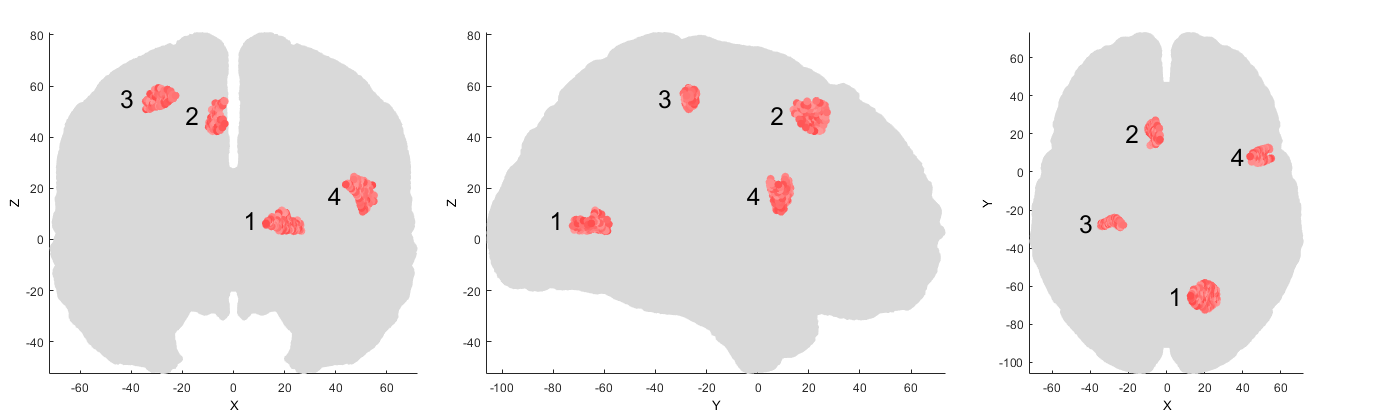
\includegraphics[width=0.989\textwidth]{figures/visualisation-groundtruth.png}
    \caption{Ground-truth locations in the brain of the simulated class-dependent signals, covering the 1.5~cm maximum deviation. In data set 1, source numbers 1 and 2 generated ERPs in one class, but not in the other. In data set 2, 1 and 2 generated alpha activity in one class, while 3 and 4 did so in the other.}
    \label{fig:visualisation:groundtruth}
\end{figure*}


\section{Methods}


\subsection{Data Simulation}

In order to have a known ground truth to evaluate the method, we used simulated EEG data. This was generated using SEREEGA \cite{krol2018sereega}, an open-source toolbox dedicated to simulating event-related EEG activity. Using the New York Head model and lead field \cite{huang2016nyhead}, two sets of 64-channel data were simulated. Each data set consisted of two conditions (classes) for the classifier to distinguish.

\paragraph{Data set 1} This data set contained systematic class differences in the temporal domain. One class consisted entirely of brown noise emanating from 64 sources spaced throughout the brain. The second class consisted of equally arranged noise, along with two event-related potentials (ERPs) emanating from two selected sources, respectively (numbered 1 and 2 in Figure~\ref{fig:visualisation:groundtruth}). The second source's ERP had an average amplitude four times greater than the other; however, this larger-amplitude ERP only occurred randomly in 25\% of epochs of that class. Single epoch amplitudes varied by 20\%. Both peaked at 300~ms $\pm$~50 with a width of 200~ms $\pm$~40.

\paragraph{Data set 2} This data set contained systematic class differences in the spectral domain. Both classes contained brown noise emanating from 64 sources spaced throughout the brain. Furthermore, each class contained additional uniform white noise filtered between 8 and 14~Hz, emanating from two sources each. In both classes, one source's signal amplitude was twice that of the other. (From Figure~\ref{fig:visualisation:groundtruth}, source numbers 1 and 2 were active in one class; 3 and 4 in the other.)

Note that the sources selected here do not reflect any deliberately chosen functional region. For the purposes of this paper, the selected regions' neuroscientific significance is not relevant: we merely wish to reconstruct their locations.

Each data set mentioned above consisted of 10 simulated `participants'. The non-noise brain source locations were relatively consistent across these participants, differing up to 1.5~cm across participants. (Note that a small shift in position can lead to a significant change in projection as, due to the cortical folds, the source will be oriented differently relative to the scalp.) The other sources were randomly distributed for each participant. A total of 100 epochs of 800~ms each were simulated for each class.

The signal-to-noise ratio was controlled in such a way that a cross-validated estimate of the classifier accuracy would roughly average 75--80\%, which are common rates for BCI applications.


\subsection{Classifier Visualisation in Putative Source Space}


\subsubsection{Separation of the Data into Sources}

We wish to visualise a classifier in putative source space. To that end, independent of any BCI classifier, the data must first be separated into putative sources. Different methods exist for this purpose. In this paper, we use independent component analysis (ICA) \cite{bell1995} as an example. ICA is a blind source separation method that decomposes the data $x$ into statistically maximally independent sources $s$ by finding a transformation or `unmixing' matrix $A$ such that $x=As$. $A$ is a filter matrix weighting the individual channel activations in sensor space to obtain the identified independent component activations. Inversely, $A^{-1}$ contains the forward model of these components, i.e., their projections onto the scalp. Other source separation methods will produce different contents of $A$, but their application in this method is essentially the same.

Independent EEG sources are dipolar \cite{delorme2012dipolar}. We can thus fit an equivalent dipole model to the forward ICA decomposition, e.g. using the EEGLAB toolbox DIPFIT 2.3 \cite{oostenveld2003dipfit}. The dipole model provides a 3D localisation for each independent component that minimises the residual variance between the dipole and the component projections.

For the results in this paper, since we used simulated data, we did not calculate $A$ on the data. Instead, we obtained the ground-truth mixing matrix directly from the simulation. The equivalent dipole model however was calculated separately using DIPFIT.


\subsubsection{Obtaining a Classifier}

The method presented here applies to linear discriminant analysis (LDA)-based spatio-temporal classifiers. In particular, we present results for common spatial patterns and the windowed-means approach.

In the windowed-means approach (WM) \cite{blankertz2011}, the mean amplitudes of the scalp activations at each electrode and in each time window are extracted as features, to which shrinkage LDA is applied to separate the classes. This results in LDA filter weights  $w_\textrm{WM}=\Sigma_\textrm{WM}^{-1}(\mu_{1}-\mu_{2})$ where $\mu_{1}$ and $\mu_{2}$ are the mean of the features for classes 1 and 2 respectively and $\Sigma_\textrm{WM}$ is the common class covariance.

Common spatial patterns (CSP) \cite{ramoser2000} are used to extract features in the frequency domain. CSP finds the optimal set of filter weights that maximise the variance of the filtered signal for one class while simultaneously minimising it for the other. Usually the top $m < \frac{C}{2}$ filters for each class are selected, where $C$ is the number of channels. The data in each epoch is spatially filtered to this new pseudo-channel space and the log of the signal's variance on each pseudo-channel is selected as the set of features for the classifier. We then apply a shrinkage LDA, resulting in LDA filter weights $w_\textrm{CSP}$. 


\subsubsection{Obtaining a Classifier's Forward Model}

In case of the WM classifier, the LDA filter weights cannot be neurophysiologically interpreted. As Haufe et al. explain, ``classifier weights can exhibit small amplitudes for measurement channels containing the signal-of-interest, but also large amplitudes at channels not containing this signal'' \cite{haufe2014}. Therefore, we must first transform the LDA filter weights into \emph{patterns}. For this paper, we did this by multiplying the LDA filter weights of the backward model by the regularised LDA's common covariance matrix (as opposed to the non-regularised version \cite{haufe2014}). Thus, the patterns $p_\textrm{WM}=\Sigma_\textrm{WM} w_\textrm{WM}=\mu_{1}-\mu_{2}$ show the differential scalp activity between classes.

For the CSP classifier, let CSP filters be columns of the matrix $W \in \mathbb{R}^{C\times C}$. CSP patterns are then defined to be columns of $P = (W^{-1})^T \in \mathbb{R}^{C\times C}$. Essentially, $P$ and $W$ are the forward and backward models, respectively. However, not each of the selected CSP filters contributes equally to classification. Their respective contributions depend on the LDA weights that were trained on their features. Here, the same LDA filter weight issues apply that were mentioned above. We thus transform these into interpretable weightings or forward weights indicating their relative contributions: $\tilde{w}_\textrm{CSP}=\Sigma_\textrm{CSP} w_\textrm{CSP}$ where $\Sigma_\textrm{CSP} \in \mathbb{R}^{2m \times 2m}$ is the common covariance of the CSP features from classes 1 and 2. We use these forward weights to scale the CSP patterns for visualisation: let $P_\textrm{sel} \in \mathbb{R}^{C\times 2m}$ be the CSP patterns corresponding to the $2m$ selected CSP filters, then the $i$-th column in $p_\textrm{CSP}$ is the $i$-th column in $P_\textrm{sel}$ scaled by the $i$-th element in $\tilde{w}_\textrm{CSP}$.  

We now have patterns representing the forward model for these classifiers in the form of weights for each electrode. For WM, we have one pattern for each time window. For CSP, we have $m$ weighted patterns for each class.


\subsubsection{Projecting the Classifier Patterns into Source Space}

The ICA's unmixing matrix $A^{-1}$ transforms sensor-level scalp activations into source activations. Similarly, it can transform sensor-level weights into corresponding weights in source space. When patterns contain class-relevant scalp projections, projecting these into source space gives us the \emph{relevance weights} $w_r=|A^{-1} p|$ that indicate how the different source activations linearly combine to create these patterns. In other words, the relevance weights reflect to what extent the sources contribute to the patterns. By extension, the relevance weights thus reflect to what extent the sources contribute to the class differences. For our purpose, the sign of the weights is not relevant at this point, hence we take the absolute value.

In case of WM, we now have one set of relevance weights per time window per participant. In case of CSP, we have  $2m$ sets per participant. Each set contains as many weights as we have independent components for that participant.


\subsubsection{Alternative Source Weights}
\label{visualisation:alternative}

Using different methods can give different perspectives on the data. We have explained how sensor-level patterns can be transformed to obtain source-level relevance weights. Alternatively, source-level weights can be calculated in source space directly, independent of the classifier. For example, we can use Pearson correlation to obtain a set of weights for the WM case.

To that end, we first repeat the feature extraction in source space, i.e., we obtain the mean of each source activation in each time window. We then calculate the correlation coefficient between these source features $F_s$ and the vector of true class labels $L$ to obtain a set of weights $w_\textrm{WMcorr} = |corr(F_s,L)|$. The sign is irrelevant for our purpose. 


\subsubsection{Visualising Relevance Weights in Source Space}

In case of WM, we generate one visualisation per time window, each illustrating the sources contributing to the class differences at that time. In case of CSP, we generate one per class, illustrating the sources distinctive for that class.

For each time window or class, respectively, the obtained relevance weights are distributed to the dipole locations of the corresponding sources for each participant. We then generate a weighted 3D kernel density plot containing these weights for all participants in one plot. For this, we use the EEGLAB plug-in dipoleDensity v0.36 \cite{miyakoshi2013dipdens} which aligns the output to slices of the mean MNI brain. For the figures in this paper, we used a smoothing kernel of 12~mm. 

\begin{figure*}[t]
    \centering
    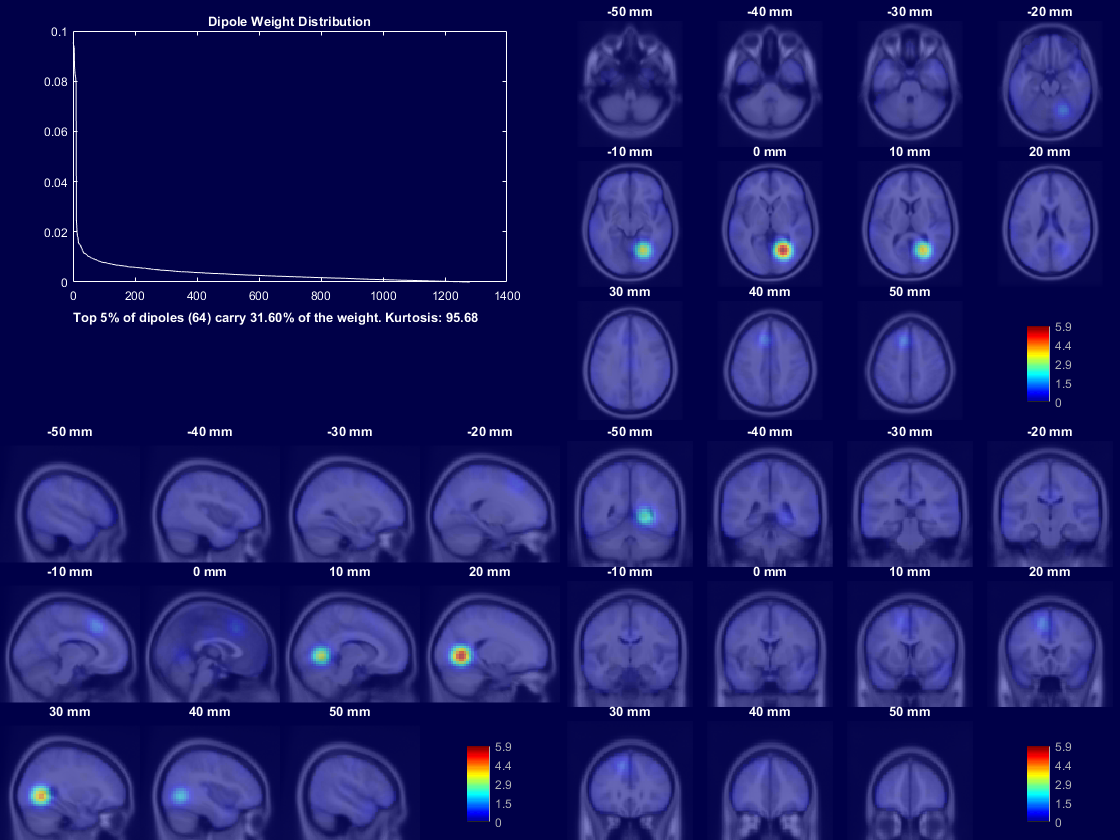
\includegraphics[width=\textwidth]{figures/visualisation-result_CSP_class2.png}
    \caption{Visualisation of the CSP classifier: class 1. Slices are labelled with their corresponding MNI coordinates. Top left: sorted dipole weight distribution.}
    \label{fig:visualisation:csp2}
\end{figure*}


\begin{figure}[t]
    \centering
    \subfloat[]{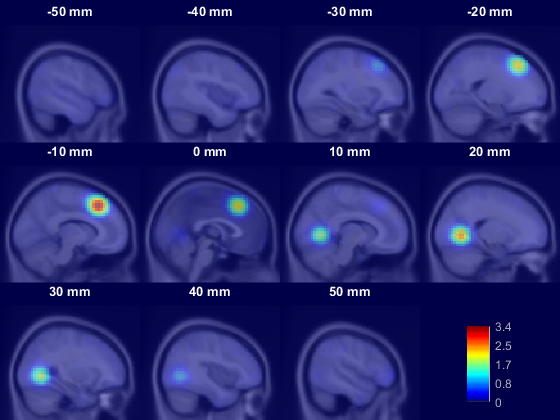
\includegraphics[width=0.45\textwidth]{figures/visualisation-result_ERP_LDA_sagittal.png}}%
    \qquad
    \subfloat[]{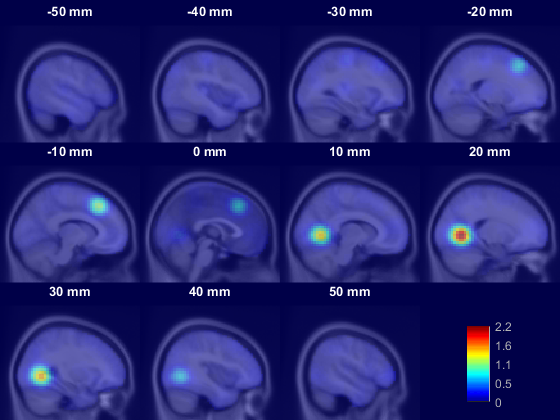
\includegraphics[width=0.45\textwidth]{figures/visualisation-result_ERP_correlation_sagittal.png}}%
    \caption{Left (a): Partial visualisation (sagittal section) of the WM classifier: projected LDA weights. Right (b): Partial visualisation (sagittal section) of source feature class correlation in data set 1: source correlation weights.}
    \label{fig:visualisation:erpldacorr}
\end{figure}

\begin{figure}[t]
    \centering
    \subfloat[]{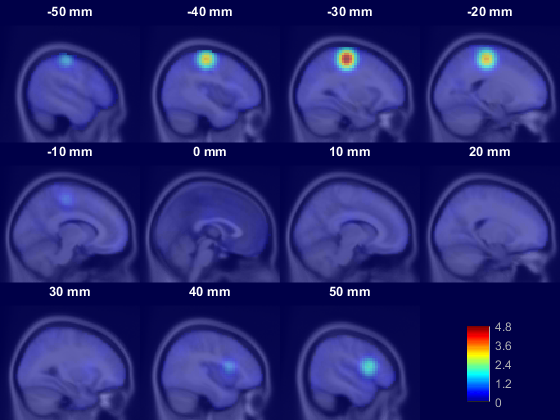
\includegraphics[width=0.45\textwidth]{figures/visualisation-result_CSP_class1_sagittal.png}}
    \qquad
    \subfloat[]{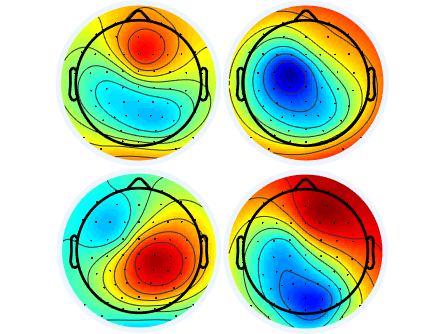
\includegraphics[width=0.45\textwidth]{figures/visualisation-erp_projections_2x2.png}}
    \caption{Left (a): Partial visualisation (sagittal section) of the CSP classifier: class 2. Right (b): Combined projection patterns of the two class-dependent sources in data set 1, for four of the simulated participants.}
    \label{fig:visualisation:csp1proj}
\end{figure}


\section{Results}

Figure~\ref{fig:visualisation:csp2} shows the output of the presented method for all participants in one case. The top left shows the sorted distribution of the relevance weights. The other panels show different slices of the mean MNI brain along with the colour-coded weighted dipole density, or `relevance density'. The sparse distribution indicates that a relatively small number of sources receive a relatively high percentage of weights. In other words, the method shows that the differences between the classes can be traced back to a relatively specific area in the brain.

Figure~\ref{fig:visualisation:csp2} visualises class 1 of the CSP classifier calibrated on data set 2. We see that the most dense, i.e. the most relevant area is near source number 1 in figure~\ref{fig:visualisation:groundtruth}. A second, weaker area of relevance is near source number 2. This accurately reflects the simulation of data set 2, where class 1 was defined by activity in these two sources, with the signal amplitude of source number 1 twice that of source number 2.

To preserve space, the other figures only show the sagittal density slices. Figure~\ref{fig:visualisation:csp1proj} (left) visualises the second class of data set 2, as identified by the CSP classifier. This accurately reflects the correct locations of source numbers 3 and 4.

Figure~\ref{fig:visualisation:erpldacorr} (left) visualises the regions of interest of the LDA classifier calibrated on data set 1 in a selected time window. This, too, accurately reflects the ground truth that sources in the right-occipital and left-frontal lobes (i.e. numbers 1 and 2 in figure~\ref{fig:visualisation:groundtruth}) were generators of the class differences. Notably, we see that the sources are weighted roughly equally, with source 2 weighted only slightly more than source 1. This is in line with the signals that were generated by these two sources. The amplitude of source 2 was four times that of source 1. However, the probability of a signal occurring at all in source 2 was only 25\%, whereas source 1 was active in each simulated trial. The mean amplitude of these sources over all trials was thus roughly the same, but their predictive value was not.

Figure~\ref{fig:visualisation:erpldacorr} (right) visualises the alternative weights for data set 1, described in section~\ref{visualisation:alternative}. We see a high correlation density for source number 1 and a significantly lower density for source number 2. This reflects the difference in predictive value between sources 1 and 2.


\section{Summary}

We simulated two data sets of 10 simulated participants each. Each participant's data was simulated with unique locations for the generator sources, with some consistency maintained for the sources that generated the class differences. In one data set, these class differences were caused by the presence of event-related potentials from two sources. In the other, differences were caused by the presence of alpha-band activity in different sources. An ICA solution was available for the simulated data.

Two different classifiers were trained on the two data sets respectively: A WM classifier, focusing on temporal differences between the classes in data set 1, and a CSP classifier, focusing on spectral differences in data set 2.

For the WM classifier, we transformed the LDA filter weights into patterns representing the forward model. For the CSP classifier, we separated the produced CSP patterns and weighted them by computed forward weights.

We then transformed these patterns into relevance weights connected to independent components using the unmixing matrix of each participant's data's ICA solution. Since a 3D position in the brain was calculated for each of these independent components, we were able to generate a `relevance density plot' indicating the classifiers' regions of interest. As we used simulated EEG data, we compared the obtained results to the known ground truth and could verify that the generated plots corresponded to the original sources.  

For the WM classifier, we also presented an alternative method to calculate relevance weights directly in source space. This method can provide a different perspective on the brain dynamics underlying the class differences.


\section{Discussion}

In our earlier work \cite{zander2016nat} we presented a combination of the two WM-based methods discussed here, where the classifier's regions of interest were additionally weighted by those regions' class-correlation. In this paper we simulated data that highlights how these two methods can provide different perspectives when used separately.

The use of simulated data enabled us to compare the method's results to a known ground truth. We see that under these circumstances, the method accurately recovers the correct sources in the brain. Of course, simulated data represents only a first test case. The previous iteration of this method has already been shown to produce results in line with hypotheses on real EEG data \cite{zander2016nat}, and we will continue this work by validating the current method on other real EEG recordings. We will also extend the method to filter-bank CSP \cite{ang2008fbcsp}, and make all code available for free.

Simulated data also allowed us to use a ground-truth ICA decomposition to initially control for the varying results that different ICA methods provide. In future work, we will furthermore apply the method to simulated data with ICA decompositions of varying quality. And, since estimating the covariance matrix is a fundamental step in producing the patterns, we will further investigate the influence of different covariance estimation methods on the patterns and their projections into source space.

The method presented here visualises the areas in the brain that the classifier focuses on, for two popular classification methods. The patterns that can be obtained from these classifiers can be neurophysiologically interpreted on their own \cite{haufe2014}. However, the current method provides two additional advantages. First of all, the patterns are decomposed into individual sources. A single pattern can consist of the combined projections of any number of different sources, and different source projections can interfere with each other to the point of making interpretation difficult. For example, figure~\ref{fig:visualisation:csp1proj} (right) shows the combined projection patterns of the two class-dependent sources in data set 1 for four of the simulated participants. As we can see, minor changes in source location and orientation produce large differences in the projection pattern. From these patterns, it is not obvious that they are produced by two distinct sources, let alone their location. With accurate ICA models, we can untangle this relation and show individual source contributions to the classifier. 

Secondly, this method uses an equivalent dipole model to visualise the sources in 3D space. Projection patterns coming from roughly the same cortical area can vary markedly between participants due to anatomical differences. A 3D visualisation of the cortical areas corrects for these differences in a way that e.g. a mean projection pattern cannot. We visualise the combined relevance weights of all participants in a single plot to highlight the most consistently relevant areas.

It is important to be able to perform an inspection of a classifier's regions of interest, and compare the results to our hypotheses as well as other perspectives on the data. When we design a BCI application, we hypothesise what functions (and thus, what regions) of the brain will be targeted. Visualisation methods such as this one enable us to compare a classifier's actual regions of interest to these hypotheses, and validate our assumptions---and to gather new insights about the cortical processes underlying the observed effects.


\section*{Acknowledgements}

This work was supported by the Deutsche Forschungsgemeinschaft (ZA 821/3-1), a Short-Term Research Grant awarded to MM by the German Academic Exchange Service, and the National Science Foundation (IIS 1528214).


\section*{References}

A shared bibliography starts at page~\pageref{bibliography}.


\clearpage
\pagestyle{plain}

        
    \part{Validations}
    \label{part:validations}
        
\chapter{Neuroadaptive Technology Enables Implicit Cursor Control Based on Medial Prefrontal Cortex Activity}
\chaptermark{Neuroadaptive Technology Enables Implicit Cursor Control}%
\label{chapter:nat}%


{\chaptermeta

\textbf{Zander, T. O.\textsuperscript{1,2,*}, Krol, L. R.\textsuperscript{1,2,*}, Birbaumer, Niels\textsuperscript{3,4}, \& Gramann, K.\textsuperscript{1,5}}

{\small
\textsuperscript{1}Biological Psychology and Neuroergonomics, Technische Universität Berlin, Berlin, Germany
\textsuperscript{2}Team PhyPA, Technische Universität Berlin, Berlin, Germany
\textsuperscript{3}Institute for Medical Psychology and Behavioural Neurobiology, University Tübingen, Tübingen, Germany
\textsuperscript{4}Wyss Center for Bio and Neuroengineering, Geneva, Switzerland
\textsuperscript{5}Center for Advanced Neurological Engineering,
University of California San Diego, San Diego, USA \textsuperscript{*}Shared first authorship

This is the postprint version of the manuscript published as follows:

Zander, T. O., Krol, L. R., Birbaumer, N. P., \& Gramann, K. (2016). Neuroadaptive technology enables implicit cursor control based on medial prefrontal cortex activity. \emph{Proceedings of the National Academy of Sciences, 113}(52), 14898–14903. doi: 10.1073/pnas.1605155114\nocite{zander2016nat}
\par}}


\abstract%
The effectiveness of today' s human–machine interaction is limited by a communication bottleneck as operators are required to translate high-level concepts into a machine-mandated sequence of instructions. In contrast, we demonstrate effective, goal-oriented control of a computer system without any form of explicit communication from the human operator. Instead, the system generated the necessary input itself, based on real-time analysis of brain activity. Specific brain responses were evoked by violating the operators' expectations to varying degrees. The evoked brain activity demonstrated detectable differences reflecting congruency with or deviations from the operators' expectations. Real-time analysis of this activity was used to build a user model of those expectations, thus representing the optimal (expected) state as perceived by the operator. Based on this model, which was continuously updated, the computer automatically adapted itself to the expectations of its operator. Further analyses showed this evoked activity to originate from the medial prefrontal cortex and to exhibit a linear correspondence to the degree of expectation violation. These findings extend our understanding of human predictive coding and provide evidence that the information used to generate the user model is task-specific and reflects goal congruency. This paper demonstrates a form of interaction without any explicit input by the operator, enabling computer systems to become neuroadaptive, that is, to automatically adapt to specific aspects of their operator' s mindset. Neuroadaptive technology significantly widens the communication bottleneck and has the potential to fundamentally change the way we interact with technology.


\clearpage


\fancypagestyle{nat}{%
    \fancyhf{}
    \fancyhead[EC]{\textit{\leftmark}}
    \fancyhead[OC]{\textit{\rightmark}}
    \fancyfoot[C]{\thepage \\ \vspace{6.8mm} \colorbox{footerbg}{\parbox{\paperwidth-2\fboxsep}{\centering\parbox{0.75\paperwidth}{\centering\fontsize{9pt}{9pt}\selectfont\textcolor{footerfg}{This is the postprint version of published manuscript: Zander, T. O., Krol, L. R., Birbaumer, N. P., \& Gramann, K. (2016). Neuroadaptive technology enables implicit cursor control based on medial prefrontal cortex activity. \emph{Proceedings of the National Academy of Sciences, 113}(52), 14898–14903.}}}}}
    \fancyfootoffset[]{1.25in}}
\pagestyle{nat}


\section{Significance}
The human brain continuously and automatically processes information concerning its internal and external context. We demonstrate the elicitation and subsequent detection and decoding of such ``automatic interpretations'' by means of context-sensitive probes in an ongoing human–computer interaction. Through a sequence of such probe-interpretation cycles, the computer accumulates responses over time to model the operator' s cognition, even without that person being aware of it. This brings human cognition directly into the human–computer interaction loop, expanding traditional notions of ``interaction.'' The concept introduces neuroadaptive technology---technology which automatically adapts to an estimate of its operator' s mindset. This technology bears relevance to autoadaptive experimental designs, and opens up paradigm-shifting possibilities for human–machine systems in general.


\section{Introduction}

In the European Union, 96\% of enterprises rely on computers for their productivity \cite{eurostatisoc_ci_eu_en2}. Advances in human-computer interaction (HCI), concerning the effective, efficient, and satisfying use of computer systems, may thus carry great societal benefits, e.g. in terms of productivity \cite{rogers2011}. However, although interaction techniques have become increasingly user-friendly---e.g. from punch cards to touch screens---they still depend on the user (operator) to translate their original thought or intention into a sequence of small, explicit commands. This translational step, where the human operator must ultimately obey the machine's logic, presents both a communication bottleneck and a source of potential error \cite{tufte1990}. At the same time, the computer has practically no limitation to the amount of information it can communicate, and is not as adaptable as its user. In these aspects, present-day HCI is asymmetrical \cite{suchman1987hmcproblems}. Comparing this to human-human interaction, \citeA{fischer2001usermodeling} emphasizes the importance of a shared understanding of the situation and an understanding of the communication partner. In this sense, for a computer system to `understand' its user, it needs a model of that user---a source of information that goes beyond the explicitly given commands. On the basis of such a model, a computer system could adapt its behavior to better suit the current mode of the user \cite{fischer2001usermodeling}. This could help alleviate the issue of asymmetry. Relevant information to that end concerns the user's intentions, subjective interpretations, and emotions. 

Four decades of developments in brain–computer interfaces (BCIs) \cite{vidal1973direct,wolpaw2012bcibook} have yielded a set of methods that may be used to obtain such information in real time, provided that this information is detectably reflected in brain activity. Specifically, BCIs can detect in real time changes in the electroencephalogram (EEG) and translate these changes into control signals, in line with the principles of physiological computing \cite{fairclough2009fundamentals}. A subgroup of BCIs, so-called ``passive BCIs'' (pBCIs) \cite{zander2011}, focuses on monitoring otherwise covert aspects of the user state \cite{zander2012context} during an ongoing HCI. Neurophysiological correlates of the above-mentioned aspects can be detected and interpreted in the context of the interaction, and can be used to inform the computer about relevant changes in the user's cognition and affect. Using pBCI, thus, a computer can in fact acquire information about its operator other than the explicitly given commands. As such, neurophysiological activity can induce appropriate changes in the machine in real time, essentially serving as an implicit command, without requiring the user to exert any conscious effort in communicating to the computer \cite{zander2011}.

Previous and present-day BCI systems use information derived about the user state in only an ad hoc fashion: momentary information derived by the BCI from the EEG is directly interpreted as a specific user intention \cite{schultzekraft2016veto,zander2010gazeinput}, situational interpretation \cite{blankertz2011}, or a change in the cognitive \cite{gerjets2014workload} or affective \cite{chanel2009emotion} state. These implementations represent one-to-one mappings of user states to machine behavior. We propose, however, that a machine using pBCI can detect both general user states and transient, event-related responses, and can use these to continuously and accumulatively learn about its operator. Specifically, we propose that the machine collates the neurophysiological responses of its operator (i.e., implicit inputs) and coregisters them against the events and contexts that evoked them. This allows the machine to build and continuously update a specific and context-sensitive model of that operator \cite{zander2012context}. The goal is to combine the information gathered from multiple responses to different events to gain insights into higher-level aspects of the operator's cognition.

One aspect of higher cognition that may be inferred in this manner is described by the theory of human predictive coding. Predictive coding holds that there exists a continuous, automatic prediction of future (neuronal) events, as well as a continuous comparison of those predictions with their corresponding final perception \cite{clark2013predictive,friston2010free,brown2011inference}. Discrepancies resulting from these comparisons inform the brain of the correctness of its predictions and actions, providing a fundamental mechanism---prediction error minimization---to shape and optimize behavior. The corresponding predictive signals are assumed to be carried by the dopaminergic system. Changes in the continuous evaluation of events and actions lead to changes in the dopaminergic input to the anterior cingulate cortex, (dis)inhibiting its neurons and eliciting a detectable response \cite{holroyd2002}. Predictions of what is expected to happen, in this sense, relate closely to what is intended to happen. This makes the correlates of predictive coding a fundamental source of information concerning user intention---an aspect of the user's cognition that is highly relevant to HCI.

In this paper, we demonstrate that by collating passive BCI output and context information, it is possible to develop, step by step, a user model that accurately reflects correlates of predictive coding and reveals task-relevant subjective intent.

Specifically, we demonstrate that a user model can be developed and used to guide a computer cursor toward the intended target, without participants being aware of having communicated any such information. Using a passive BCI system, the participant's situational interpretations of cursor movements were classified and interpreted, in the given context, as directional preferences. A user model was generated to represent these context-dependent directional preferences, and this model was then used to guide the cursor toward the intended movement direction.


\section{Results}

The experimental paradigm involved a form of cursor control. The cursor moved discretely over the nodes of a (4$\times$4 or in later stages 6$\times$6) grid. For each movement the cursor could travel up to eight directions, horizontally, vertically, and diagonally, to one of the adjacent nodes. Each movement served both to move the cursor and to elicit a neurophysiological response, reflecting the subjective correctness of that movement. In essence, each movement thus also served as a probe for information. One of the grid's corners was designated the target. For each movement, it could thus be determined at what angle of deviance relative to the target the cursor had moved. This was used for an objective interpretation of the cursor's behavior. We describe the paradigm in detail in SI Appendix.

The event-related potential (ERP) following each probe (i.e., each cursor movement) is shown in Fig. \ref{fig:nat:figure1}\emph{a}. A one-way analysis of variance of the systematic peak differences around 180 ms indicated a significant main effect of angular deviance from the target direction on peak amplitude [\textit{F}(7,126) = 47.243, \textit{P} < 0.001]. Specifically, the peak amplitudes (Fig. \ref{fig:nat:figure1}\emph{b}, upper curve) differed significantly (\textit{P} < 0.001) between both the lowest and the highest angular deviation from the target direction as used by the classifier. In between, the peak amplitudes scaled linearly with angular deviance, as fitted by a linear regression model using each group's mean angular deviance as a predictor (slope coefficient \textit{b} = −0.0035, \textit{F} = 45.28, \textit{P} < 0.001; \textit{R$^{2}$} = 0.33). Further posthoc comparisons corrected for false discovery rate additionally indicated that significant differences between adjacent groups (\textit{P} < 0.05) were found mostly for groups of lower angular deviance, whereas differences between the three largest-deviance groups (124$^{\circ}$ and up) were not significant. The results of all posthoc comparisons are listed in SI Appendix, Table S3. In summary, the probe elicited systematic variations in event-related amplitudes, depending on the goal congruency of the presented stimulus.

\begin{figure}[ht]
    \centering
    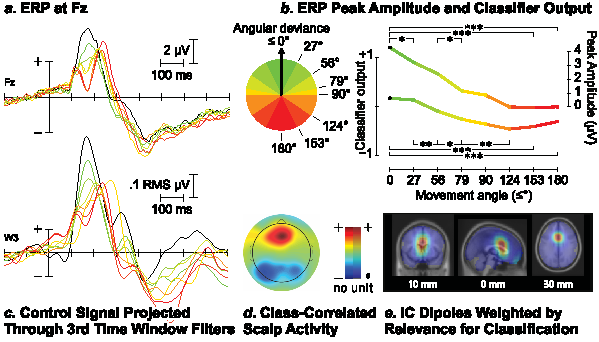
\includegraphics[width=\textwidth]{figures/nat-figure1.pdf}
    \caption[Neurophysiological analysis.]{Neurophysiological analysis. (a) Grand average ERP at Fz (\textit{n} = 19) time-locked to cursor movement, divided into eight groups depending on angular deviance. (b) Peak amplitudes around 180 ms for the ERP in A, and mean classifier output for cursor movements sorted by angular deviance with selected significant differences indicated (\textit{***P} < 0.001, \textit{**P} < 0.01, \textit{*P} < 0.05). (c) Grand average ERP (\textit{n} = 19) projected through the sources focused on in the third time window (150–200 ms; indicated in gray). (d) Scalp map of difference-between-classes activity that contributed to classification in the third time window. (e) Source localization for the third time window.}
    \label{fig:nat:figure1}
\end{figure}

To enable real-time detection of the individual, single-trial neuroelectric responses, we calibrated a discriminative classification system. Calibration was based on two classes of responses representing the extreme ends of the spectrum, with angular deviances of 0$^{\circ}$ making up the one class, and angular deviances of ≥135$^{\circ}$ the other (Fig. \ref{fig:nat:figure2}\emph{a}). This classification system used a subject-dependent linear combination of all 64 available channels, taking into account full scalp information. It automatically generated appropriate spatial filters for eight 50-ms time windows---starting at 50 ms after stimulus presentation---using supervised machine learning and linear discriminant analysis. This set of filters weighted each electrode in each time window, depending on its relevance to classification. The recorded signal projected through them thus allowed an optimal discrimination between the two classes. This projected recorded signal---from all 64 channels, between 50 and 450 ms after stimulus presentation---defined the control signal. The feature extraction is described in more detail in SI Appendix.


\begin{figure}[ht]
    \centering
    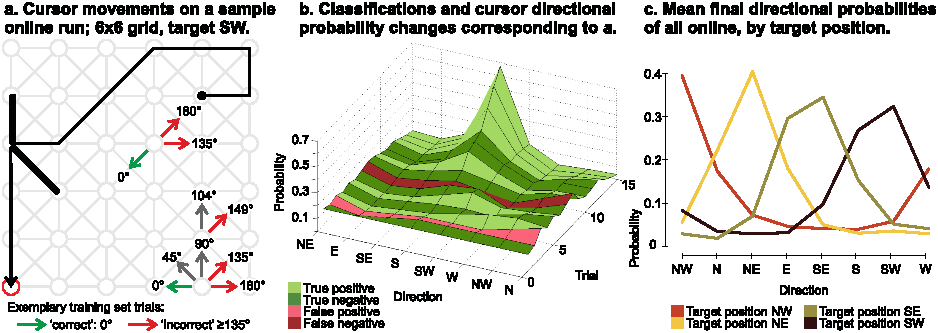
\includegraphics[width=\textwidth]{figures/nat-figure2.pdf}
    \caption[Cursor behavior and user model generation.]{Cursor behavior and user model generation. (a) Sample online cursor movements. Also indicated: selected movement directions, their relative angular deviance, and class membership (calibration phase). Movements with an angular deviance >0$^{\circ}$, <135$^{\circ}$ (e.g., gray arrows) were not in the training set. (b) User model evolution during the movements in A based on movement classifications. Ground truth is taken from button presses. (c) The mean final user model representing the directional probabilities/preferences upon reaching the target, grouped by absolute target position.}
    \label{fig:nat:figure2}
\end{figure}

The resulting classification system not only provided a filtered discriminative control signal; it also allowed us to investigate which cortical sources the system focused on. Based on this information, conclusions can be drawn about the discriminative cognitive processes underlying the classification. Fig. \ref{fig:nat:figure1}\emph{c–e} shows an analysis of the features used for classification between 150 and 200 ms, highlighting the relevant factors in this time window: the discriminative scalp activity, the source localization of this activity within the brain, and a projected ERP of the signal generated from the identified sources. SI Appendix, Fig. S5 and Movies S1 and S2 present this same analysis for the full time course under investigation. See SI Appendix, Fig. S8 for scalp maps of the class-specific activity in each time window.

This approach identified a specific neuroanatomical area across participants: The system based its decisions on neuronal activity that predominantly originated in the medial prefrontal cortex (mPFC). The classification system was trained only on two binary classes representing the smallest and largest angular deviances. Back-projection of the signal through the system's filters, however, reveals that the classification system optimally identified the same sources that generated the linear modulations seen in the grand average ERP. Following the pattern found for the peak amplitudes at Fz, peak amplitudes of the projected ERPs differed significantly (\textit{P} < 0.001) between the classes used by the classifier. In between, the peak amplitudes scaled linearly with angular deviance, as fitted by a linear regression model of the aggregated means, using each group's mean angular deviance as a predictor (\textit{b} = −0.0019, \textit{F} = 31.9, \textit{P} = 0.011; \textit{R$^{2}$} = 0.91). Statistically significant differences between adjacent groups also followed a similar pattern; see SI Appendix, Table S5 for all pairwise comparisons. It is thus clear that the classification system focused on a response that reflected the probe's logic.

The signal thus carried task-relevant information. For a true test of this signal's single-trial reflection of individual judgments of cursor movements, and thus its usefulness in creating a user model describing subjective intent, we created a closed-loop, online version of the original offline paradigm. Following each single cursor movement, an individually calibrated classification system classified the evoked response. The extracted information was used for reinforcement learning on the side of the cursor \cite{sutton1998reinforcementlearning}, modifying the probabilities of upcoming cursor movements such that the cursor would be more likely to go toward the target if the classifications were correct. The resulting probability statistics can then be understood as a user model, describing the user's preferred behavior of the cursor. This description's accuracy is then reflected in the user model's success in enabling effective, goal-oriented control of the cursor.

Performance was operationalized as the number of cursor movements required to reach one target. Because even a completely randomly moving cursor would eventually reach the target, three conditions were distinguished: random, online, and ``perfect.'' In the random condition, no reinforcement took place and the cursor merely moved randomly. In the online condition, the cursor was reinforced based on the classifications of the classification system. The perfect condition was simulated: the cursor already knew the location of the target and reinforced itself with 100\% accuracy, although it did proceed to move probabilistically. This condition represents the best possible performance given the constraints of the grid and the cursor's movement algorithm.

The offline calibration data were gathered on a 4$\times$4 grid. The online, closed-loop system was tested on both a 4$\times$4 grid, and on a theretofore unseen 6$\times$6 grid. Performance results are summarized in Fig. \ref{fig:nat:figure3}.

\begin{figure}[ht]
    \centering
    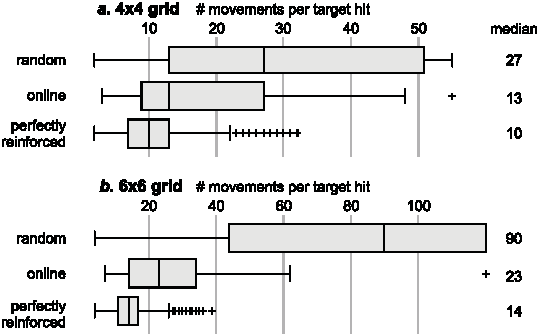
\includegraphics[width=0.64\textwidth]{figures/nat-figure3.pdf}
    \caption[Performance measure distributions for nonsupported, online, and perfectly reinforced cursor movements on the two online grid sizes.]{Performance measure distributions for nonsupported, online, and perfectly reinforced cursor movements on the two online grid sizes. (a) Performance on the 4$\times$4 grids. (b) Performance on the 6$\times$6 grids. All differences between the three conditions are significant (\textit{P} < 0.025). Whiskers cover $\pm$2.7$\sigma$.}
    \label{fig:nat:figure3}
\end{figure}

On the 4$\times$4 grid, a randomly moving cursor required an average of 27 movements. In the simulated condition of perfect performance, this number dropped to 10. When the cursor was reinforced online, an average of 13 steps was required---a significant improvement compared to the random condition (\textit{P} < 0.025) bridging the gap toward the perfect condition by 82\%.

On the 6$\times$6 grid random cursor movement required 90 steps on average, and 14 in the perfect-accuracy simulation. Even though no training data had been gathered from the 6$\times$6 grids, the online system bridged this gap by 88\%, requiring 23 movements on average (\textit{P} < 0.01).

On both grids, the online performance also differed significantly from the perfect performance (\textit{P} < 0.025).

Movie S3 shows a number of online cursor movements and illustrates the adaptive paradigm's responses.

Online application thus significantly increased the goal congruency, confirming that the signal the classification system focused on was situationally relevant. Although the cursor only made binary interpretations of the classifier's output, this output was continuous: a scale, from −1 to +1, correlating to the movements' degree of goal congruency. This is illustrated in Fig. \ref{fig:nat:figure1}\emph{b} (lower curve). The classifier output differs significantly (\textit{P} < 0.001) between the classes used by the classifier. In between, the classifier output scaled linearly with angular deviance, as fitted by a linear regression model using each group's mean angular deviance as predictor (\textit{b} = 0.0035, \textit{F} = 295.42, \textit{P} < 0.001; \textit{R$^{2}$} = 0.76). See SI Appendix, Table S4 for further comparisons.

Even though the linearly scaled information was not taken into account, binary classifications still resulted in a graded user model, describing the appropriateness of the different cursor movements depending on the intended target's position. To illustrate this, Fig. \ref{fig:nat:figure2}\emph{a} visualizes the cursor's movements over a grid during one of the online runs with the target in the southwest corner. Fig. \ref{fig:nat:figure2}\emph{b} shows how the individual directional preferences/probabilities in the user model are updated after every cursor movement, showing the progression toward a clearly identified preference for the southwest corner. Fig. \ref{fig:nat:figure2}\emph{c} illustrates the mean final user models for all participants for the four different target positions. It is clear that the user models accurately represent the intended target position. The mean final user model across all participants is illustrated in SI Appendix, Fig. S4, with statistics in SI Appendix, Table S2. SI Appendix, Fig. S9 shows one more example of online cursor behavior.


\section{Discussion}

We have demonstrated that binary classifications of subjective interpretations of cursor movements can be aggregated into a user model reflecting, in the given context, directional intent. Based on this model, the cursor was effectively guided toward the target. Participants were not aware of their influence on the cursor. Although not used explicitly in this study, analysis shows that more fine-grained information may be available in the elicited responses, encoded in the linear dependency of the response on the angular deviance.

An approach combining independent component analysis (ICA, \citeNP{bell1995,makeig1996}), supervised machine learning, and higher-order statistics not only gave insight into the individual single-trial responses, but also enabled error-minimized source localization and signal back-projection as well as real-time single-trial analysis. These characteristics could be used to validate the classification system as well as the user model. Firstly, the online application of the classification system increased the paradigm's goal congruency to near the optimum: The gap from no reinforcement to optimal reinforcement could be bridged by over 80\% using the presented classification system, both on the 4$\times$4 grid and on the theretofore unseen 6$\times$6 grid. This significant reduction in the number of steps required to reach a target provides evidence that the classification of brain responses following a cursor movement was based on task-relevant information: Each movement indeed elicited a response enabling the identification of subjective directional preferences.

Secondly, the neurophysiological analysis, based on the classification system's filter set, revealed that the underlying signal predominantly stemmed from the mPFC, and reflected the experimental paradigm's logic. Further interpretation of the neurophysiological response points to its likely generator process. Given the signal's time course, its localization, and the evoking stimuli, the response is in line with the framework of predictive coding. We hypothesize that in the present study, participants consistently predicted---for lack of information that would indicate otherwise---that the cursor would perform the only action that would have been appropriate, i.e., that it would move in the direction of the target. Interestingly, however, our findings imply an extension of the general framework of predictive coding. A focus on ``negative'' signals is central to current interpretations and findings related to predictive coding: Indications of discrepancies, of prediction errors, are seen as central to learning by reinforcement, in turn explaining the large range of rich human behavior and intelligence \cite{hawkins2004intelligence}. The sensitivity of the ERP amplitude to the quality of the cursor movements, however, seems to indicate that neural activity generated within the mPFC provides a range of graded responses to both positive and negative movements. In this context, these reflect the observer's directional preferences, modeling an important, task-relevant factor of their subjective cognition. This points to a continuous response range within the mPFC that not only detects deviations from a predicted event to adapt future behavior, but also confirms correct predictions to reinforce adequate behavior or sharpen perceptive hypotheses. This activity thus reflects complex aspects of the operator's cognition, and can be highly informative for external systems that have access to it.

Taken together, these results demonstrate effective cursor control through implicit interaction: While participants were unaware of having any influence on the cursor, the presented stimuli elicited informative neuronal responses that allowed the system to establish a user model from which the participants' intentions could be derived. The computer system adapted its behavior to fit this model---thus becoming neuroadaptive. The necessary information could also have been provided explicitly and volitionally, but conscious interpretation can involve any number of additional considerations and processes (e.g., resolving competing interpretations from different judgment strategies), and would require an explicit decision as well as its translation into a command to inform the machine. Direct access to such interpretations circumvents these time-consuming and effortful steps, proving advantageous even with simple binary decisions, as implemented here. Communicating more fine-grained information, as seems also to be available, would be even more difficult using traditional input techniques, but equally effortless using the method presented here. As such, neuroadaptive technology based on passive BCI bypasses the communication bottleneck present in traditional HCI, effectively widening it by allowing interaction to take place through implicit channels. This decreases the asymmetry present in current HCI paradigms.

At this point, we would like to speculate about possible implications and future extensions of the findings and the line of thought presented here. Our current method essentially quantified subjective directional preferences, supplying a single value that indicated, in the given context, whether a person interpreted a single cursor movement as being supportive of reaching the target or not. This can be seen as a real-time assessment of subjective satisfaction/dissatisfaction with the presented probe stimulus, thus allowing the generation of a user model representing subjective intent. Interestingly, one can imagine a computer system that intelligently decides what probe to present, to gather information. A system with an incomplete user model, for example, could present a probe to gauge the user's response and thus gather the missing information. Such an act of active learning \cite{settles2009activelearning} would invert the traditional HCI cycle: The probe may be understood as a command---a request for feedback---direct from the machine to the user's brain, inducing its own interpretation, which results in the machine indeed receiving the requested feedback. In the demonstration presented here, each cursor movement served as such a probe, and allowed the gradual development of a user model, but a more intelligent selection of probes may improve the system's efficiency.

With such a fundamental process as for example predictive coding underlying a neuroadaptive system, a large scope of potential applications can be imagined. Any process or path that can be divided into a sequence of one-dimensional (e.g., positive–negative) responses could potentially be covered implicitly (SI Appendix, Fig. S10). And, as human predictive coding shows, a great deal can be achieved based on such information using, for example, the relatively simple process of reinforcement. The 2D grid used here could be replaced by any n-dimensional space representing different system parameters. It is tempting to envision how such neuroadaptive systems could transform work and leisure activities in everyday settings. An implementation analogous to the current demonstration (but going beyond the currently presented results), using affective interpretations rather than cognitive ones \cite{zander2009affective}, could be an adaptive, open-ended electronic book. While reading, the reader would interpret the story as it unfolded, thus automatically responding to events with a detectable affective state. Based on what the reader apparently finds enjoyable, a neuroadaptive system could then change the content of subsequent pages. With a sequence of such adaptations, the story is gradually steered in the reader's preferred direction. However, the reader would not actively be directing the story, and would not even need to be aware of the system's existence.

Similarly, the general method demonstrated here is of value to neuroadaptive experimental paradigms. Such paradigms can use the real-time feedback supplied by the classification system to adapt to individual strategies, rather than enforcing a uniform logic over all participants. Probe stimuli can be used to first inspect the subjective relevance of different experimental aspects, for example, and then adaptively go into detail, presenting more fine-grained nuances of these aspects, to model how they influence the brain dynamics of that individual.

A word of caution is in order. Neuroadaptive systems can be said to be systems with an agenda, having a goal of their own \cite{fairclough2009fundamentals}. By autonomously initiating each interaction cycle using a specifically selected probe stimulus, they would be in a position to ``guide'' the interaction such that specific information can be gathered, and to change the interactive experience based on that or other information. When designing such systems, care should be taken that this agenda is not adverse to the user's intention. Furthermore, the fact that it can rely on automatic, unconscious responses represents a potential danger to informed consent. Users should always have access to full information concerning the system's goals and actions.

The benefits of closed-loop neuroadaptive technology, however, may be vast. It enables experimental paradigms to model and adapt to relevant individual aspects in real time. For technology in general, this concept could represent a paradigm shift in that it skips translational effort, grants the machine initiative and agency, and may even function outside of conscious awareness. This offers designers the prospect to completely rethink the notion of interaction and the possibilities offered by it. In almost a century of neurophysiological research, a number of correlates of cognitive processes have been identified in the EEG, some of which can already be detected in single trials using passive BCI methodology (as, e.g., \citeNP{schultzekraft2016veto,blankertz2011,gerjets2014workload,chanel2009emotion,protzak2013gazebased,zander2011}). We are looking forward to investigating which of these could be meaningfully elicited and interpreted to inform personalized user models, as per the concept of neuroadaptive technology presented here. Commercial systems and experimental paradigms specifically designed for this type of implicit interaction---a cybernetic convergence of human and machine intelligence---could offer new functionality and scientific results we cannot currently foresee.


\section{Materials and Methods}

\subsection{Experimental Procedure and Setup}

All participants were informed of the nature of the experiment and the recording and anonymization procedures before signing a consent form. The Ethics Committee of the Department of Psychology and Ergonomics at the Technische Universität Berlin approved the experiment and the procedures.

A gray grid was shown on a black background, with a red target node indicated in one of the grid's corners, and a red circular cursor visible on one of the nodes (Fig. \ref{fig:nat:figure1}\emph{a} and SI Appendix, Fig. S1). The cursor's starting position on each grid was one node away from the corner opposite the target's, in a straight line to the target. In each trial, the cursor moved from its current node to one of the adjacent nodes. A 1-s animation within the cursor served as a countdown. The cursor would then instantaneously jump to the next node, highlighting in white its new position and the grid line between the two nodes. This configuration remained visible for 1 s. Following that, the highlights disappeared and the cursor would remain at its new position for 1 s more before the next trial. Movie S4 shows animated stimuli as seen by the participant.

Throughout the experiment, participants were instructed to judge each individual cursor movement as either ``acceptable'' or ``not acceptable'' with respect to reaching the target, and to indicate their judgment by pressing either ``v'' or ``b,'' respectively, on a computer keyboard using the index finger of one hand. These button presses were logged by the system but were not used as input.

EEG was recorded using 64 active Ag/AgCl electrodes mounted according to the extended 10–20 system. The signal was sampled at 500 Hz and amplified using BrainAmp DC amplifiers (Brain Products GmbH).

Participants first performed 5 blocks of 120 trials on grids of 4$\times$4 nodes. If the target had not been reached after 55 trials in one grid, a new grid was started. Fifty-five is twice the median number of random movements required to reach a target on a 4$\times$4 grid. The EEG recorded during these five blocks served to calibrate the classifier, as discussed below. In online sessions, this classifier was then applied to one more block of 120 trials on 4$\times$4 grids, and one last block of 120 trials on 6$\times$6 grids. No maximum number of trials other than the block's length was set for the 6$\times$6 online blocks.

During calibration blocks, the cursor moved randomly. During online application of the pBCI, the directional probabilities were altered based on the classification of each movement as either ``correct'' or ``incorrect,'' biasing the cursor to repeat movements classified as correct.

A total of 19 participants participated in this study, with an average age of 25.4 y ±3.4. Seven were female. All had normal or corrected to normal vision. The first 3 only performed offline calibration trials, whereas the following 16 additionally performed online trials.

Additional details are provided in SI Appendix.


\subsection{Classifier}

A classifier was individually calibrated on data from the initial 600-trial recording of random cursor movements. Movements with an angular deviance of 0$^{\circ}$ were labeled as class 1, and movements with an absolute deviance of 135$^{\circ}$ or more were labeled as class 2. A regularized linear discriminant analysis classifier was trained to separate classes \cite{blankertz2011}.

The open-source toolbox BCILAB \cite{kothe2013bcilab} version 1.01 was used to define and implement the pBCI. Features were extracted through the windowed means approach, using the average amplitudes of eight sequential time windows of 50 ms each, between 50 and 450 ms after each cursor movement \cite{blankertz2011}. For this feature extraction, the data were first resampled at 100 Hz and band-pass filtered using fast Fourier transform from 0.1 to 15 Hz. Ensuring that the features were independent and identically distributed, a 5$\times$5-times nested cross-validation with margins of 5 was used to select the shrinkage regularization parameter, and to generate estimates of the classification system's online reliability.

Additional details are provided in SI Appendix.


\subsection{Identifying Scalp Projections}

Following \citeA{haufe2014}, linear discriminant analysis (LDA) patterns $A=(a_j)_j$ were generated for each participant from the LDA filters $M=(m_j)_j$ originally used for online classification by conjugation with the features' covariance matrix $C: A=CMC^{−1}$. Spatial interpretation of these patterns for each time window reflects a mixture of scalp activations related to discriminative source activity $\hat{A}=(\hat{a}_j)_j$ and class-invariant noise representation $N$, with $A=\hat{A}+N$. The latter was filtered out by weighting each pattern entry $a_j$ with the correlation of its associated feature activity vector over trials $F_j$ to the binary vector of true class labels $L: \hat{a}_j=corr(F_j,L) \cdot a_j$ The resulting correlated pattern $\hat{A}=(\hat{a}_j)_j$ can be visualized by topographic plots for each time window, as in Fig. \ref{fig:nat:figure1}\emph{d}.

Additional details are provided in SI Appendix.


\subsection{Localization}

The classification model used was a multivariate approach, an LDA, optimized for the discriminability of the extracted features between classes. Each feature represents data at a single sensor for one of the chosen time windows. Hence, applying the methodology recently introduced by \citeA{haufe2014} interprets the classification model at sensor level, and reveals further insight into the relevant underlying processes.

To identify the sources producing the signal, the backward model, i.e., the LDA filter, was combined with an ICA. The ICA unmixing matrix $W=(I_1,I_2,\cdots,I_n)$ was determined on manually cleaned data for each participant by using the Adaptive Mixture ICA (AMICA) Toolbox \cite{palmer2012amica}, such that $s = Wx$, where $s$ represents the source activation related to a given scalp activation $x$. For each time window, the relevance for classification $R_i$ of each independent component $I_i$ can then be determined by distributing the LDA filter weights to the independent components via $W$, weighted by two factors. The first factor compensates for the amplitude alignment of the LDA filter weights to the feature amplitudes. It is determined by calculating the variance over trials of the feature $\hat{F}_i$ extracted from the time series of the independent component: $Vi = var(\hat{F}_i)$. A second weight is determined for filtering out noise representations by weighting the independent components with the correlation of their feature activity to the true class labels (as described above for electrode activity): $R_i=V_i* corr(\hat{F}_i,L) * WM$.

To then localize these sources, equivalent dipole models that describe the most likely position of the source in a standard head model were identified for selected components by using the EEGLAB plug-in DIPFIT 2.x \cite{oostenveld2003dipfit}. Components were selected by a threshold criterion for residual variance (RV) of the dipole model (RV < 0.15) and visual inspection of the activation spectra, time courses, and scalp topographies. Only dipolar components clearly reflecting cortical, ocular, or muscular activity were included in the analysis. For every time window, each of the 371 resulting dipoles was weighted by the relevance $R_i$ of its associated independent component. The areas of high relevance were then described by a weighted dipole density plot using the EEGLAB plug-in dipoleDensity \cite{miyakoshi2013dipdens} by plotting the dipole density per cubic millimeter weighted by the relevance $R_i$ of each included dipole with a smoothing kernel of 12 mm.

Movie S2 shows the results of this analysis for the full time course under investigation.

The above-mentioned process of dipole selection did not markedly influence the analysis. Compared with all 1,191 dipoles and averaged over the 8 time windows, the 820 rejected dipoles (68.8\%) carried 7.5\% of the weights distributed by the classifier. Relative to all 1,191 dipoles, a total of 87 dipoles received a relevance weight larger than an SD of 1 in at least one of the time windows. These 7.3\% of dipoles carried 77.8\% of the total weight distributed by the classifier. Four of these highly weighted dipoles (4.6\%) were rejected in the process explained above and not included in the analysis. These four represent 1.7\% of the weight included in the analysis. Three belonged to the same subject.

Additional details are provided in SI Appendix.


\subsection{Performance Measures and Statistical Methods}
Cursor performance was operationalized as the number of movements required to reach the target. Only completed grids are included in the analysis, i.e., either when the target was hit or the maximum number of trials was reached. Online, this latter event occurred a total of seven times to seven participants on the 4$\times$4 grids, and to two participants on the larger grids. Out of 120 cursor movements per grid size per participant, this resulted in 88 pBCI-supported target hits for the smaller grid, and 47 for the larger one.

Random cursor movement data are nonparametrically distributed and vary greatly. Therefore, we used a resampling approach where the available sample of pBCI-supported measures was repeatedly compared with a new random sample of the same size of nonsupported performance measures, using a Wilcoxon rank-sum test. Out of 50,000 such comparisons, 98\% of tests were significant at $\alpha$ = 0.025 for the smaller grid; for the larger grid, 100\% of tests were significant at this level.

The perfect performance was simulated by automatically reinforcing the cursor as in the online sessions, with all movements with an angular deviance of less than 45$^{\circ}$ reinforced positively and all others negatively. The same procedure as above yielded significant differences to the pBCI-supported measures for both the 4$\times$4 grid (99.9\% of tests significant at $\alpha$ = 0.025) and the 6$\times$6 grid (100\%).


\section*{Acknowledgements}

We thank S. Haufe, S. Makeig, M. Miyakoshi, J. Faller, and C. Wienrich for contributions to the various stages of the research process and C. Kothe, S. Jatzev, M. Rötting, and Brain Products GmbH for support. Part of this work was supported by the Human Factors and Ergonomics Society Europe Chapter VRC Corporation Exchange Grant (Reference EC/2014.11).
Additional details are provided in SI Appendix.


\section*{References}

A shared bibliography starts at page~\pageref{bibliography}.


\clearpage
\pagestyle{plain}

        
\chapter{Investigating the Separation of Salience and Valence in Implicit Cursor Control}
\chaptermark{Salience versus Valence}%
\label{chapter:salval}%


{\chaptermeta 

\textbf{Krol, L. R.\textsuperscript{1}, Pawlitzki, J.\textsuperscript{1} \& Gramann, K.\textsuperscript{1,2,3}, \& Zander, T. O.\textsuperscript{4}}

{\small
\textsuperscript{1}Biological Psychology and Neuroergonomics, Technische Universität Berlin, Berlin, Germany
\textsuperscript{2}School of Computer Science, Faculty of Engineering and Information Technology, University of Technology Sydney, Sydney, Australia
\textsuperscript{3}Center for Advanced Neurological Engineering, University of California San Diego, San Diego, CA, USA
\textsuperscript{4}Zander Laboratories B.V., Amsterdam, the Netherlands

This is a preprint version of the manuscript submitted as:

Krol, L. R., Pawlitzki, J., Gramann, K. \& Zander, T. O. (submitted). Investigating the separation of salience and valence in implicit cursor control. \textit{Proceedings of the National Academy of Sciences}.
\par}}


\abstract%
Implicit cursor control based on medial prefrontal cortex (mPFC) activity was demonstrated in 2016 \cite{zander2016nat}: neuroadaptive technology based on passive brain-computer interfacing enabled participants to essentially steer a cursor towards a highlighted target without these participants being aware of doing so. Such forms of implicit interaction can potentially enable a wide range of neuroadaptive applications, depending on which cognitive and affective processes can be reliably targeted by the classifiers that decode the corresponding brain activity. The mPFC activity in question was assumed to reflect predictive processes influenced by top-down biases informed by the participants' subjective intentions to reach the target. However, since the target was visually highlighted, it is conceivable that perceptual processes, which may be agnostic to the meaning of the visual stimuli, played a role as well. Here, we use classifier visualisation in 3D source space and an adapted experimental design to disentangle the contributions of perceptual salience- and subjective valence-related processes in implicit cursor control. We show that the two processes are both present in the data. The visualisation method allows them to be separated and localised in different cortical areas, with visual processing primarily situated in parietal areas and valence-related processing predominantly in the mPFC. This also demonstrates that neuroadaptive technology can indeed access subjective valence-related processes for implicit control.


\clearpage


\fancypagestyle{salval}{%
    \fancyhf{}
    \fancyhead[EC]{\textit{\leftmark}}
    \fancyhead[OC]{\textit{\rightmark}}
    \fancyfoot[C]{\thepage \\ \vspace{9.9mm} \colorbox{footerbg}{\parbox{\paperwidth-2\fboxsep}{\centering\parbox{0.75\paperwidth}{\centering\fontsize{9pt}{9pt}\selectfont\textcolor{footerfg}{This is a preprint version of submitted manuscript: Krol, L. R., Pawlitzki, J., Gramann, K. \& Zander, T. O. (submitted). Investigating the separation of salience and valence in implicit cursor control. \textit{Proceedings of the National Academy of Sciences}.}}}}}
    \fancyfootoffset[]{1.25in}
}
\pagestyle{salval}


\section{Introduction}

A brain-computer interface (BCI) allows a measurement of a person's brain activity to be interpreted in real time and used as input to a computer, essentially providing a new communication channel that does not depend in any way on muscular activity \cite{wolpaw2012newsun}. While the focus of BCI research has long been on medical applications, for example offering paralysed patients the ability to communicate with the outside world or control parts of their environment \cite{birbaumer2006commcontrol,vansteensel2016alsimplant},
the scope of BCI technology has significantly widened in roughly the past decade with hard- and software solutions now being offered even to the general public \cite{ienca2018brainleaks}. Of particular note is the category of so-called \emph{passive} BCI systems (pBCI; \citeNP{zander2011,krol2018interactivity}), which are different from other categories of BCI in that they derive output from brain activity that was not specifically modulated for communication or control. Instead, pBCI decodes a person's naturally occurring brain activity, thus revealing aspects of their naturally occurring mental states. This decoded \emph{implicit input} can potentially be obtained without the user's explicit voluntary cooperation \cite{schmidt2000,rotting2009implicit,zander2014implicit}. As such, a pBCI could for example allow a smart car to detect its driver's state of drowsiness and automatically pull over without requiring the drowsy driver to make any explicit decisions \cite{zander2017dry}, or allow adaptive systems to respond to different levels of their users' mental load without adding any additional load to it \cite{yuksel2016bach,ewing2016tetris,zander2017surgery}. Such systems using implicit input in order to adapt themselves, e.g. for control or interaction, are referred to as neuroadaptive technology \cite{zander2016nat}.

In the context of human-computer interaction, the operator's naturally occurring brain activity is largely dependent on current task parameters. Neuroadaptive technology can automatically adapt these parameters in order to support the human operator, but conversely, it can also pro-actively change these parameters in order to induce specific mental states, or to learn from the brain activity resulting from specific changes. For example, rather than increasing or decreasing automation levels in response to rising or lowering levels of workload \cite<e.g.,>{byrne1996adaptiveauto}, a system could actively cycle through a set of possible task configurations in order to evaluate which produces the optimal level of load. This method is called cognitive probing \cite{krol2020cognitiveprobing}.

In an earlier work, we demonstrated how cognitive probing can be used to enable implicit cursor control \cite{zander2014implicit,zander2016nat}. Where traditional forms of BCI can enable users to steer a cursor by actively producing different mental states (most commonly, this is motor imagery; \citeNP{pfurtscheller2001motorimagery}), the implicit cursor control paradigm started with a cursor that was moving autonomously, but randomly, across the nodes of a grid. One of the corners of this grid was visually highlighted to represent the target, i.e., the supposed goal of the cursor's movements. Participants were instructed to judge each individual cursor movement as being either `appropriate' or not with respect to reaching the indicated target. The results showed significant differences between (appropriate) cursor movements going towards the target, and (inappropriate) movements leading the cursor away from the target. Furthermore, this difference was classifiable with an estimated single-trial accuracy of 72\%. We could thus use this classifier output in real time as implicit input, in order to reinforce the initially random cursor movements to gradually guide the cursor towards the target. When brain activity indicated that a movement was appropriate, the probability of moving again in that same direction was increased, and conversely, the corresponding probability was decreased after each movement that was classified as inappropriate. This produced significantly goal-directed behaviour of the cursor, purely on the basis of brain activity elicited by each and every movement. A similar concept was demonstrated by \citeA{iturrate2015teaching}. We emphasise, however, that in \citeA{zander2016nat}, the participants were unaware of having any influence on the cursor's movements, hence this being an example of implicit control.

An analysis of the signal underlying classification in this implicit cursor control experiment revealed the relevant cognitive processes to stem predominantly from the medial prefrontal cortex (mPFC). In particular, inappropriate movements elicited a strong negativity visible at channel Fz around 180~ms. This and various additional findings led to these results being interpreted within the framework of predictive coding: the brain's automatic, constant prediction of future sensory input in order to optimise behaviour by minimising prediction errors \cite{friston2010free,clark2013predictive}. Processes with a similar time course, spatial distribution, and cortical origin have been identified to be involved in the realisation of having committed an error \cite{falkenstein1990,falkenstein2000}, receiving feedback concerning previous errors \cite{miltner1997,holroyd2003frn}, receiving feedback concerning erroneously executed commands \cite{ferrez2008simulated,mousavi2017mi}, and observing others commit errors \cite{miltner2004,schie2004}. Their many similarities have resulted in the assumption that these negativities are generated by the same system, but under different circumstances; in particular, the \emph{error-related negativity} is said to follow actively committed errors, while the \emph{feedback-related negativity} follows the display of performance-related feedback \cite{walsh2012frnreview}. An account based on reinforcement learning has therefore been postulated which holds that a generic error-processing mechanism exists, in which changes in the dopaminergic input to the anterior cingulate cortex (ACC) indicate whether or not predictions have been met \cite{holroyd2002,nieuwenhuis2004rlern}. At the scalp, this activity is then reflected as a negativity in case of events being worse than predicted, and/or a positivity when events are better than predicted \cite{holroyd2008rewardpositivity}. 

Therefore, we hypothesised that participants in the implicit cursor control paradigm predicted that the cursor would move towards the target, with correct movements towards the target (i.e., positive feedback) yielding the known positivity and incorrect movements the corresponding negativity. In the absence of any informative cues with respect to upcoming cursor movements, the participants' intentions or preferences pertaining to the cursor movements thus determined how each movement was predicted and interpreted. As such, higher-order cognitive functions (here: intentions or preferences) could be inferred from lower-level processes (predictive error signals). Such lower-level processes may be difficult to consciously control, with potentially far-reaching implications for the privacy of thought \cite{mecacci2019criteria}.

The feedback-related negativity is generally considered to be a binary signal reflecting the processing of positive or negative outcomes, influenced by motivational involvement but not by reward or error magnitude \cite{yeung2004passiveactivefrn,hajcak2006binaryfrn}. Interestingly, the negativity observed in the implicit cursor control paradigm showed a linear dependency on the `appropriateness' of the cursor movements, as measured by their angular deviance from a straight line towards the target. This hinted at the involvement of a cortical process that not only signals deviations from predicted events in order to improve future behaviour, but in fact confirms or rejects predictions in a graded way in order to e.g. reinforce adequate behaviour or sharpen perceptive hypotheses. Combined with the above-mentioned assumption that these predictions are informed by higher-level cognition, this process would then essentially reflect a subjective degree of goal attainment.

However, this interpretation assumes that there indeed was no other information available---even false information---to base a prediction on. As mentioned, in the implicit cursor control experiment the desired target was visually highlighted, thus potentially making this a form of information: it is visually more salient than other nodes in the grid, and thus, it is conceivable that perceptive processes would interpret this as a reference point regardless of its valence. It is conceivable that a `default' prediction is for one salient object (the cursor) to move towards another salient object (the target).

In light of this, a more nuanced perspective has been suggested to interpret the detected event-related potentials (ERPs) \cite{cockburn2018rewardpositivity}. Holroyd and colleagues make a distinction between surprise- or salience-related signals on the one hand, the response of which is modulated by the expectancy of events \cite{holroyd2002}, and the \emph{reward prediction error} signal on the other hand, which responds most strongly to unexpected (i.e. surprising, salient) events but whose sign is inverted for positive versus negative events \cite{sambrook2015rewardprediction}. This has primarily been investigated in the context of tasks where a positive event would for example indicate correct performance or monetary reward on a timing or gambling task, but may also apply to implicit cursor control. In short, while the different valence of movements towards and away from the target should result in a classifiable signal, the visual salience of these same movements towards or away from the highlighted node may confound these results. It thus remains an important unanswered question to what extent the signal that allowed classification may also have ``[manifested] as a specific interaction between outcome valence and outcome probability'' \cite{heydari2016rewardorsalience}, or indeed, may be explained exclusively by one or the other.

To be specific, we understand `salience' in the context of implicit cursor control to represent the perceptual (here: visual) properties of the cursor movements relative to the visually salient point of the grid. `Valence' on the other hand is the meaning imparted upon these movements by the participants as informed by the instructions, leading participants to see some movements as `appropriate' (positive valence) and others as `inappropriate' (negative valence). Because salience and valence of the cursor's movements were coupled in the original implicit cursor control experiment, it was not possible for these two factors to be differentiated. We therefore conducted a similar but adapted experiment where the visual stimuli and the participants' task were designed to allow such a differentiation to be made. In the updated design, visual stimuli were left constant between two conditions that differed only with respect to the given instructions. These instructions manipulated the valence of the visually identical stimuli. 

If processes related to visual salience were the sole or primary cause of the effects seen in the original paradigm, we should see the same effects in this experiment in both conditions. Conversely, if valence-related processes were primarily driving the results, we would expect to see an inverse pattern between the two conditions. In case both of these dimensions play a role, as is most probable, the updated experimental design allows us to compare valence parameters while isolating or controlling for visual parameters, and vice versa. This would allow us to identify which cortical areas primarily contribute to these two aspects. Here, we would expect salience to be localised primarily in occipital/parietal regions, and valence in the mPFC as per the original results.

Aside from further elucidating the neurophysiology of error- and feedback-related processing, it is important to investigate salience- and valence-related processes in the context of neuroadaptive technology. A classifier that responds only to physical (e.g. visual, salience) parameters while being agnostic to more subjective cognitive processes may have a limited number of applications in the real world. On the other hand, when a system does have access to its user's subjective (valence-related) processing, care must be taken that both this access and the gathered information is handled with due care---among other things, keeping in mind the necessity for informed consent and the value of privacy. See \citeA{krol2020cognitiveprobing} for a discussion on the ethical implications of some forms of neuroadaptive technology, which are all the more pertinent when subjective interpretations can inform the adaptations, as opposed to more `neutral' cognitive processes such as perception.


\section{Methods}

\subsection{Participants and Set-Up}

A total of 24 participants participated in the study (10 male; 22 right-handed; mean age $26.6\pm3.9$). All signed a written informed consent form. 64-channel EEG was recorded at 5000~Hz using BrainAmp DC amplifiers (Brain Products GmbH, Gilching, Germany), with active electrodes arranged on actiCAP electrode caps according to the extended international 10-20 system, referenced to FCz. Participants were seated in front of a 27'' computer display placed approximately 1~m away from them. Five participants were later excluded from the analysis due to data quality or recording issues, leaving 19 datasets (9 male; 17 right-handed; mean age $26.6\pm4.3$).


\subsection{Experimental Paradigm}

The experimental paradigm largely followed the original implicit cursor control experiment \cite{zander2014implicit,zander2016nat}, but with adaptations to allow salience and valence to be manipulated as independent variables. This required a different grid layout, shown in figure~\ref{salval:fig:grid}.

\begin{figure}[t]
    \centering
    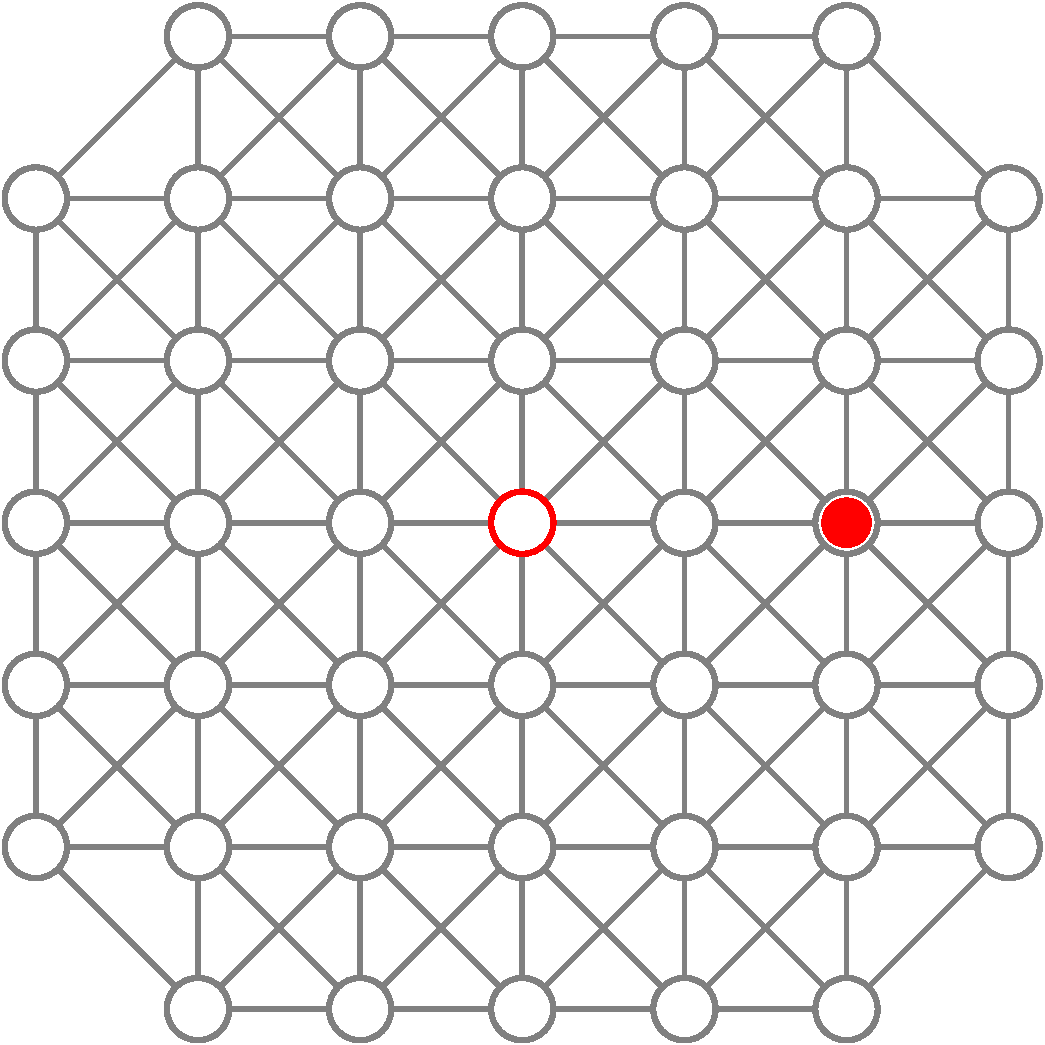
\includegraphics[width=0.5\textwidth]{figures/salval-grid.pdf}
    \caption{The grid layout as seen by the participants, with the cursor at one of four possible starting positions. The centre node was always visually highlighted.}
    \label{salval:fig:grid}
\end{figure}

The original experiment used a square grid with one of the corners bearing particular relevance (e.g., the target). On such a grid there is always an opposite corner that may, inversely, be interpreted as having particular relevance as well, being the furthest away from said target. In other words, instructions that assign positive or negative valence to one corner, may be mentally translated as assigning inverted valence to the opposite corner instead. Because of this, we instead used a larger $7\times7$ grid allowing us to place the reference node at the centre, and removed the corner nodes to eliminate any `opposite' candidates. All grid nodes were grey, open circles connected by grey lines. The reference node was a red, open circle. The cursor was a red, filled circle, somewhat smaller than the nodes. The background was black.

Starting two nodes away from the centre in a horizontal or vertical line, the cursor would move randomly to any of the up to eight adjacent nodes at a rate of one movement every three seconds. Each movement first consisted of a 1-second animation of a growing white `ghost' circle inside the cursor's red circle. This allowed the participants to predict the timing of the upcoming move. Upon reaching the same size as the cursor's red circle, the ghost cursor instantaneously moved to the next node while the red cursor remained. The grid line between these two points was highlighted in white, clearly indicating the movement between the previous and new cursor positions. This remained visible for 1 second. Following this, the red cursor instantaneously moved to the new position while the white elements disappeared. The red cursor remained at this position for 1 second before the next anticipatory animation started. (A video of this animation is available in \citeNP{zander2016nat}.)

In order to manipulate valence, there were two conditions: an `attraction' and a `repulsion' condition, defined relative to the reference node in the centre. In the attraction condition, participants were instructed that the cursor \emph{should} reach the centre node, and that reaching it should be seen as a success. If the cursor had not reached the centre after 50 movements, this was to be seen as a failure. These instructions reflected those of the original experiment. In the negative condition, the instructions were reversed: the cursor should \emph{not} reach the target, and was given 25 movements to either fail or succeed. The difference in the maximum number of movements was to even out the number of successes and failures per condition. After success or failure in either case, the grid was restarted with a different cursor starting position. The order of the two conditions was counter-balanced across participants. 

The two conditions inverted the valence of the otherwise visually identical stimuli: what was `appropriate' in one condition was `inappropriate' in the other. Participants were instructed to observe each cursor movement and label it as either `appropriate' or `inappropriate' given the current condition through a button press before the next movement occurred, i.e. within three seconds. Speed was not emphasised. Participants were given no explicit instructions as to what exact criteria to use for each judgement, but they were told that each judgement was to be made for the individual cursor movement, independent of the larger history of cursor movements. These individual cursor movements were the unit of analysis in this experiment.

Participants observed and evaluated a total of 800 cursor movements per condition for 1600 movements in total. Self-paced breaks were given between grids.

The cursor moved randomly throughout the experiment. There was no condition using online implicit cursor control.


\subsection{Independent Component Analysis}

Using EEGLAB 14.1.2b \cite{delorme2004eeglab}, the raw EEG data was subsampled to 250~Hz and band-pass filtered between 1 and 100~Hz. Channels were rejected using \texttt{clean\_rawdata}. Removed channels were spherically interpolated, and the data was re-referenced to the common average while maintaining full rank by first re-inserting the all-zero reference channel \cite{miyakoshi2017fullrankaveref}. After manually removing sections of the data highly contaminated by artefacts, two passes of independent component analysis (ICA; \citeNP{makeig1996}) were performed. A first pass yielded reliable identification of eye-related independent components (ICs), which were then removed to allow automated cleaning of the data without this algorithm erroneously identifying eye-related activity as noise. With noise sections identified, these were removed from the earlier dataset still containing eye activity, and a second pass of ICA yielded the decomposition used for further analysis.

The ICA algorithm used was AMICA \cite{palmer2012amica}, stopping either when convergence was reached or after 2000 iterations. The automated cleaning algorithm, described in more detail by \citeA{gramann2018heading}, first filtered the data between 1 and 40~Hz, and took the absolute value of the Hilbert transform of each channel. It then looked at 1-second non-overlapping time segments, and first removed any segment where a flat line occurred for more than 100~ms. Following this, all segments were ranked by their mean absolute amplitude across channels, their standard deviation across channel means, and their Mahalanobis distance from a distribution spanning all segments using the channel means as coordinates. The top 10\% of segments sorted by their mean rank, plus a 500-ms margin on either side, were then removed from the data.

The resulting ICs were dipole-fitted using DIPFIT 2.x \cite{oostenveld2003dipfit} matched to an MNI average head model. The EEGLAB plug-in ICLabel \cite{piontonachini2019iclabel} was used to identify components. Only `brain' components were kept, defined as having a residual variance of less than 15\% and a `brain' probability of at least 67\%. Non-brain components were removed. For a cluster inspection, the remaining brain ICs were clustered based on their dipole positions (relative weight in the preclustering array: 10), ERP activities (weight 1), and scalp maps (weight 1). Clustering was done using k-means producing 15 clusters, with an outlier threshold at 3 standard deviations.


\subsection{Classification}
\label{salval:sec:methods:classification}

The experiment essentially resulted in $2\times2$ classes: each movement could be categorised by visual salience as either going `towards' or `away' from the centre, or by valence as either being `good' or `bad' in the given condition. `Towards' and `away' were defined using the movements' angular deviance from a straight line towards the centre. For example, a movement with an angular deviance of $0^{\circ}$ goes directly towards the centre; a movement with an angular deviance of $180^{\circ}$ moves in a straight line away from the centre. Following calculations regarding class separability depending on different definitions of `towards' and `away', done on the first eight participants \cite{krol2019saliencevalence}, movements having an angular deviance of $\leq27^{\circ}$ were labelled as going `towards' the target, while $>117^{\circ}$ were `away'. The attraction condition thus contains \emph{good-towards} and \emph{bad-away} movements, whereas the repulsion condition contains \emph{good-away} and \emph{bad-towards} movements.

Classification was implemented using BCILAB \cite{kothe2013bcilab}. After downsampling the data to 100~Hz and band-pass filtering it between 1 and 15~Hz, we used a windowed-means approach \cite{blankertz2011} taking the mean amplitude on all channels in twelve non-overlapping 50-ms time windows ranging from 0 to 600~ms as features. This large range was chosen to include both early perceptual and later semantic processing. Linear discriminant analysis (LDA; \citeNP{bishop2006}) was used to calibrate the classifier. Five-fold random cross-validation was used to estimate classifier accuracy. Since all four classes were equalised by randomly eliminating trials from larger classes, this whole procedure was repeated five times and the reported values represent the mean across iterations.

We always classified one class of movements against one other. Within conditions, this would thus be good-towards versus bad-away for the attraction condition (Att.), and bad-towards versus good-away for the repulsion condition (Rep.). These classifications combine both valence and salience factors. To separate them, four additional classifications were performed: good-towards versus bad-towards (TvT) and good-away versus bad-away (AvA) to focus on valence differences between visually identical movements, and good-towards versus good-away (TvA+) and bad-towards versus bad-away (TvA--) to focus on the visual differences while controlling for valence.


\subsection{IC Relevance Weighting and Classifier Visualisation}

The method described in detail by \citeA{krol2018classvis} was used to obtain so-called relevance weights for each IC. In short, the channel-level spatial filter weights produced by each classifier, representing the classifier's backward model, were first transformed into forward-model patterns \cite{haufe2014}. These patterns represent the projected activity of the signals isolated by the classifier. Using the unmixing matrix obtained from the ICA, these patterns were translated into source-level weights, indicating, for each IC in each of the classifier's time windows, to what extent it contributed to classification. These so-called relevance weights were normalised across time windows within participants.

Given the dipole model fitted to each IC, the IC relevance weights can be visualised in 3D source space. Using the dipoleDensity EEGLAB plug-in \cite{miyakoshi2013dipdens}, each IC's position in the average brain volume was weighted according to its relevance to classification. We then generated a weighted 3D kernel density plot containing these weights for all participants in one figure, using a smoothing kernel of 10~mm. The scales in these images are relative, as they intend to bring physiological rather than quantitative differences into focus.

% The relevance weights can also be used to generate a weighted source-level ERP reflecting the time series of the activity isolated by the classifier. To generate these, each IC time series was weighted by the IC's relevance weight, and the weighted IC activations were summed together within subjects.


\section{Results}

\subsection{Behavioural Data}

In the attraction condition, the cursor made an average of $28.4\pm3.9$ movements per grid; in the repulsion condition, this was $19.0\pm5.1$ movements per grid. The definitions used to define the `towards' and `away' classes (i.e. `appropriate' and `inappropriate' movements) resulted in a roughly similar total of 388 movements towards, and 343 away across conditions. Grand average reaction times for the button presses were $690\pm153$~ms and $731\pm175$~ms in the attraction and repulsion condition, respectively. A within-participants permutation test with 10000 permutations found that 13 participants showed significant differences ($\alpha=0.05$, Bonferroni-corrected) in their reaction times between conditions; in all these cases, the repulsion condition had longer reaction times. For the other six, no significant differences were found. We furthermore investigated reaction time differences between two groups of participants, separated by which condition was presented first. The attraction-first group was shown the attraction condition first, and the repulsion condition second; the repulsion-first group was shown the repulsion condition first, and the attraction condition second. We performed this analysis in order to detect or rule out any order effect. Permutation tests with 10000 permutations revealed no significant differences between groups for each of the condition (all $p>0.64$).


\subsection{Independent Component Analysis}

Keeping only cortical components left on average $14.2\pm4.3$ ICs per participant. For an impression of the distribution of these ICs and as a reference for the later classifier visualisation, these ICs were clustered using k-means clustering in EEGLAB 14.1.2b \cite{delorme2004eeglab} using the same information available to the classifier---the ERPs and scalp maps, each with weight 1---and the dipole locations, with weight 10, with the threshold for outliers set at 3 standard deviations. Figure~\ref{salval:fig:clusters} shows both the dipole distribution and the scalp maps of the clusters.

\begin{figure}[htb]
    \centering
    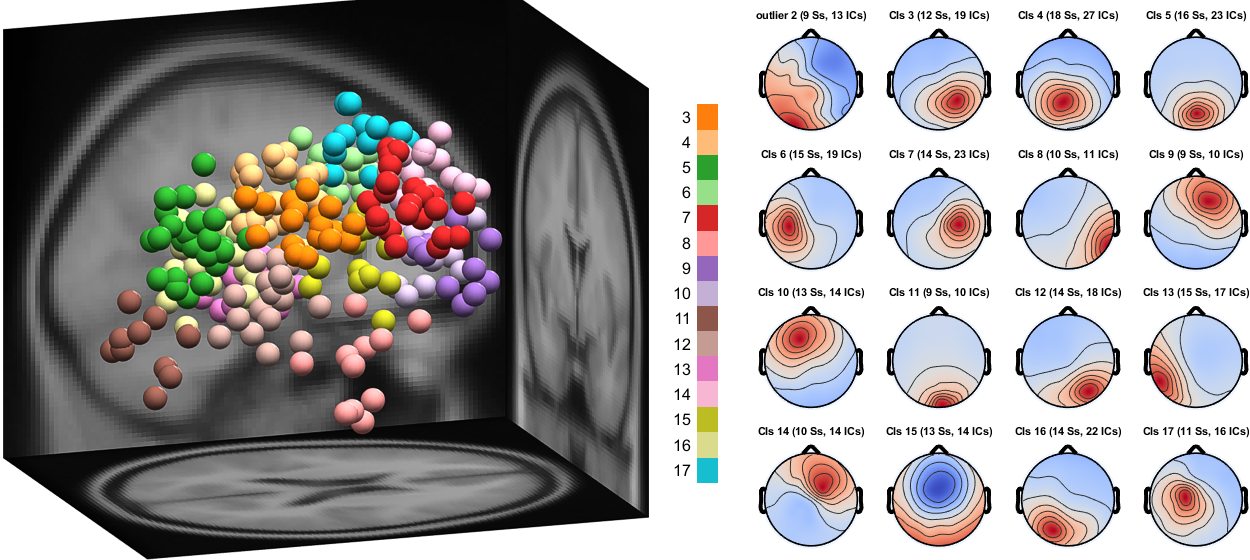
\includegraphics[width=\textwidth]{figures/salval-clusters.png}
    \caption[Independent component dipoles and cluster scalp maps.]{\emph{Left:} All 257 cortical ICs, colour-coded for each cluster, excluding 13 outlier ICs. \emph{Right:} The mean scalp maps of all 15 clusters, plus the outlier cluster.}
    \label{salval:fig:clusters}
\end{figure}


\subsection{Classification}

Table~\ref{salval:tab:bci} contains the cross-validated accuracy estimations for the six different classification schemes, using only cortical ICs. Removing non-brain ICs reduced the classification accuracy by a moderate 2.24 percentage points on average, a reduction which was nonetheless significant in most cases following paired-sample t-tests (Att $p=0.300$, Rep $p=0.011$, TvT $p=0.002$, AvA $p=0.001$, TvA+ $p=0.001$, TvA-- $p=0.003$). Still, classification accuracies for the vast majority of participants remained significantly above chance. Since the number of trials for each class was equalised, chance level is at 50\%. Classification rates that are significantly better than chance, adjusted for the number of trials \cite{mullerputz2008random}, are indicated in the table.


\begin{table}[p]
    \renewcommand{\arraystretch}{0.85}
    \centering
    \begin{tabular}{rllllll}
        \textbf{Participant}& \textbf{Att}       & \textbf{Rep}       & \textbf{TvT}      & \textbf{AvA}      & \textbf{TvA+}     & \textbf{TvA--}    \\
        1$^r$               & 85{\tiny$^{***}$}  & 68{\tiny$^{***}$}  & 63{\tiny$^{***}$} & 67{\tiny$^{***}$} & 80{\tiny$^{***}$} & 80{\tiny$^{***}$} \\
        2$^a$               & 66{\tiny$^{***}$}  & 61{\tiny$^{***}$}  & 57{\tiny$^{*}$}   & 59                & 69{\tiny$^{***}$} & 69{\tiny$^{***}$} \\
        3$^r$               & 77{\tiny$^{***}$}  & 64{\tiny$^{***}$}  & 62{\tiny$^{***}$} & 55{\tiny$^{***}$} & 74{\tiny$^{***}$} & 74{\tiny$^{***}$} \\
        4$^a$               & 80{\tiny$^{***}$}  & 75{\tiny$^{***}$}  & 67{\tiny$^{*}$}   & 67{\tiny$^{***}$} & 81{\tiny$^{***}$} & 81{\tiny$^{***}$} \\
        5$^r$               & 76{\tiny$^{***}$}  & 68{\tiny$^{***}$}  & 57{\tiny$^{***}$} & 59{\tiny$^{**}$}  & 70{\tiny$^{***}$} & 70{\tiny$^{***}$} \\
        6$^a$               & 88{\tiny$^{***}$}  & 74{\tiny$^{***}$}  & 70{\tiny$^{***}$} & 77{\tiny$^{***}$} & 78{\tiny$^{***}$} & 78{\tiny$^{***}$} \\
        7$^r$               & 82{\tiny$^{***}$}  & 66{\tiny$^{***}$}  & 60{\tiny$^{***}$} & 62{\tiny$^{***}$} & 71{\tiny$^{***}$} & 71{\tiny$^{***}$} \\
        8$^a$               & 78{\tiny$^{***}$}  & 60{\tiny$^{***}$}  & 65{\tiny$^{***}$} & 61{\tiny$^{***}$} & 72{\tiny$^{***}$} & 72{\tiny$^{***}$} \\
        10$^r$              & 72{\tiny$^{***}$}  & 61{\tiny$^{***}$}  & 65{\tiny$^{***}$} & 70{\tiny$^{***}$} & 55{\tiny$^{*}$}   & 55{\tiny$^{***}$} \\
        11$^a$              & 76{\tiny$^{***}$}  & 66{\tiny$^{***}$}  & 58{\tiny$^{**}$}  & 57{\tiny$^{**}$}  & 76{\tiny$^{***}$} & 76{\tiny$^{***}$} \\
        13$^r$              & 84{\tiny$^{***}$}  & 65{\tiny$^{***}$}  & 62{\tiny$^{***}$} & 61{\tiny$^{***}$} & 77{\tiny$^{***}$} & 77{\tiny$^{***}$} \\
        14$^a$              & 71{\tiny$^{***}$}  & 56                 & 66{\tiny$^{***}$} & 63{\tiny$^{***}$} & 68{\tiny$^{***}$} & 68{\tiny$^{**}$}  \\
        15$^a$              & 86{\tiny$^{***}$}  & 68{\tiny$^{***}$}  & 67{\tiny$^{***}$} & 64{\tiny$^{***}$} & 79{\tiny$^{***}$} & 79{\tiny$^{***}$} \\
        16$^r$              & 69{\tiny$^{***}$}  & 60{\tiny$^{***}$}  & 59{\tiny$^{***}$} & 58{\tiny$^{**}$}  & 73{\tiny$^{***}$} & 73{\tiny$^{***}$} \\
        17$^a$              & 78{\tiny$^{***}$}  & 69{\tiny$^{***}$}  & 65{\tiny$^{***}$} & 71{\tiny$^{***}$} & 68{\tiny$^{***}$} & 68{\tiny$^{***}$} \\
        20$^r$              & 85{\tiny$^{***}$}  & 59{\tiny$^{***}$}  & 66{\tiny$^{***}$} & 66{\tiny$^{***}$} & 73{\tiny$^{***}$} & 73{\tiny$^{***}$} \\
        21$^a$              & 69{\tiny$^{***}$}  & 58{\tiny$^{**}$}   & 56{\tiny$^{*}$}   & 56{\tiny$^{*}$}   & 69{\tiny$^{***}$} & 69{\tiny$^{***}$} \\
        22$^r$              & 82{\tiny$^{***}$}  & 70{\tiny$^{***}$}  & 61{\tiny$^{***}$} & 68{\tiny$^{***}$} & 76{\tiny$^{***}$} & 76{\tiny$^{***}$} \\
        24$^r$              & 59{\tiny$^{***}$}  & 61{\tiny$^{***}$}  & 63{\tiny$^{***}$} & 61{\tiny$^{***}$} & 71{\tiny$^{***}$} & 71{\tiny$^{***}$} \\
        \textbf{Mean}       & \textbf{77}        & \textbf{65}        & \textbf{63}       & \textbf{63}       & \textbf{73}       & \textbf{71}       \\
        \textbf{Mean sig.}  & \textbf{77}        & \textbf{66}        & \textbf{64}       & \textbf{66}       & \textbf{74}       & \textbf{71}       \\
    \end{tabular}
    \caption[Classification accuracies.]{Classification accuracies (\%) for the separability of the following classes. Att: towards v away in the attraction condition, i.e. good-towards v bad-away; Rep: towards v away in the repulsion condition, i.e. bad-towards v good-away; TvT: towards v towards across conditions, i.e. good-towards v bad-towards; AvA: away v away across conditions, i.e. good-away v bad-away; TvA+: towards v away with positive valence across conditions, i.e. good-towards v good-away; TvA--: towards v away with negative valence across conditions, i.e. bad-towards v bad-away. For the participants, \emph{a} or \emph{r} indicate that the attraction or repulsion condition was presented first, respectively. Significance is indicated as *~$\scriptstyle{p<0.05}$, **~$\scriptstyle{p<0.01}$, ***~$\scriptstyle{p<0.001}$. Mean sig. indicates the mean accuracy taking only those participants with $\scriptstyle{p<0.001}$.}
    \label{salval:tab:bci}
\end{table}

Separation between the classes is significantly better for Att than for Rep ($p<0.001$ using paired-sample t-tests). TvT does not significantly differ from AvA ($p=0.275$), nor does TvA+ from TvA-- ($p=0.047$). Att is significantly better than the four mixed-condition classification schemes (TvT $p<0.001$, AvA $p<0.001$, TvA+ $p<0.001$, TvA-- $p<0.001$); Rep is significantly worse than TA+ ($p=0.001$) and TA-- ($p<0.001$) but does not differ significantly from TvT ($p=0.758$) or AvA ($p=0.956$). 

Also here, we investigated differences between the attraction-first and repulsion-first groups in order to detect or rule out any order effect. Permutation tests with 10000 permutations comparing the accuracies of six classification schemes across groups revealed no significant differences (all $p>0.26$).

\begin{figure}[p]
    \centering
    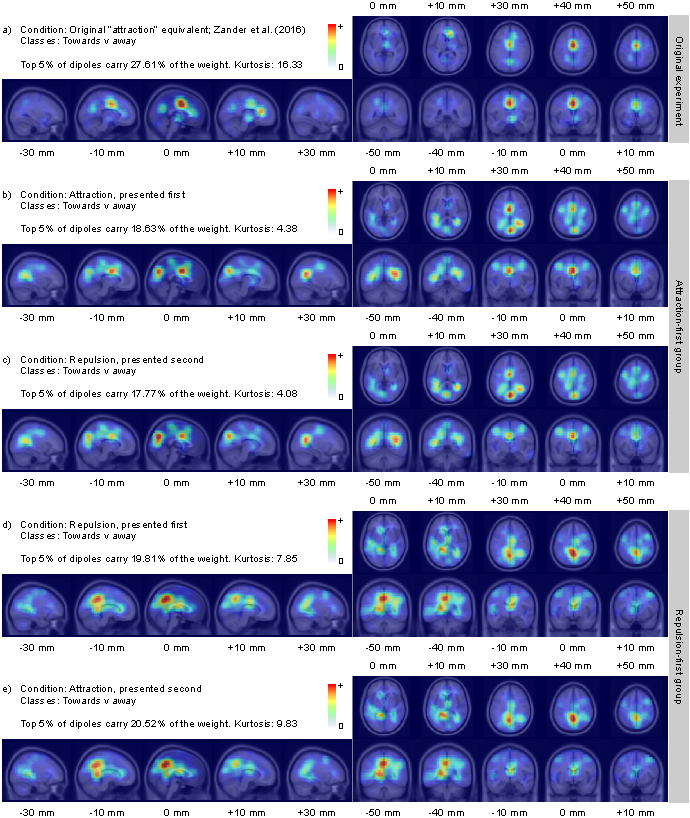
\includegraphics[width=\textwidth]{figures/salval-wdd-within.pdf}
    \caption[Weighted dipole density plots for the within-condition classifiers.]{Weighted dipole density plots showing the relevance of cortical areas to \emph{a} the original implicit cursor control experiment's classifier, \emph{b} the Att classifier for participants who saw the attraction condition first, \emph{c} the Rep classifier for the same group, \emph{d} the Rep classifier for participants who saw the repulsion condition first, and \emph{e} the Att classifier for the same group.}
    \label{salval:fig:wdd-within}
\end{figure}


\subsection{Single-Condition Classifier Visualisation}

Figure~\ref{salval:fig:wdd-within} illustrates the source-localised relevance weights for the Att and Rep classifiers, as well as for the classifier from the original implicit cursor control experiment for comparison. These figures thus show which cortical sources contributed to the separability of the classes within conditions. For increased sensitivity, each plot only includes participants for whom the respective classifier was significantly above chance at $\alpha=0.001$. Since an effect is visible here depending on which condition was presented first, the attraction-first and repulsion-first groups are separated accordingly.

Panel \emph{a} shows the relevant areas for the original experiment's classifier, equivalent to the attraction condition in this study. Panel \emph{b} and \emph{c} show the relevant areas for the current experiment's attraction and repulsion condition, respectively, but only for those participants who saw the attraction condition first. Panels \emph{d} and \emph{e} show the repulsion and attraction condition, respectively, for the remaining participants who saw the repulsion condition first. Note that all five of these classifiers combine both salience and valence dimensions. 

For the attraction-first group, the relevant cortical areas for the Att classifier largely overlap with the Att-equivalent classifier of the original experiment. There is a clear focus on the mPFC, a second focus on the centro-parietal region, albeit larger than in the original experiment, plus an additional weaker focus localised in the right-lateral parietal cortex. For the Rep classifier of the first group, these same three areas remain active, now with a stronger parietal focus than for the Att classifier.

For the repulsion-first group, for both Att and Rep classifiers, the same general centro-parietal area carries most weight with virtually no difference between the two conditions.

Interestingly, while participants within each of the two groups consistently showed relevant activations in the same areas for both conditions, the area that almost exclusively contributed to classification in the repulsion-first group, is virtually absent in any classifier of the attraction-first group, and vice versa. Given this stark difference between the two groups depending on the order of presentation, we separate the further analysis between the two groups. We will focus on the attraction-first group, as this group more closely resembles the reference data with which we wish to compare the current results. The same analysis for the repulsion-first group is provided in Section~\ref{salval:sec:results:repulsionfirst}.


\subsection{Event-Related Potential at Fz}

Figure~\ref{salval:fig:posfirst-erp-channel} shows the scalp ERP at channel Fz for the processed data, i.e., referenced to the common average, with non-cortical contributions removed, and filtered between 1 and 15~Hz. The attraction condition (when presented first), on the left panel, reproduces the result from the original experiment with a peak negativity following (negative-valence) movements away from the centre node at around 180~ms, versus a peak positivity at that same time for (positive-valence) movements towards the centre. 

\begin{figure}[htb]
    \centering
    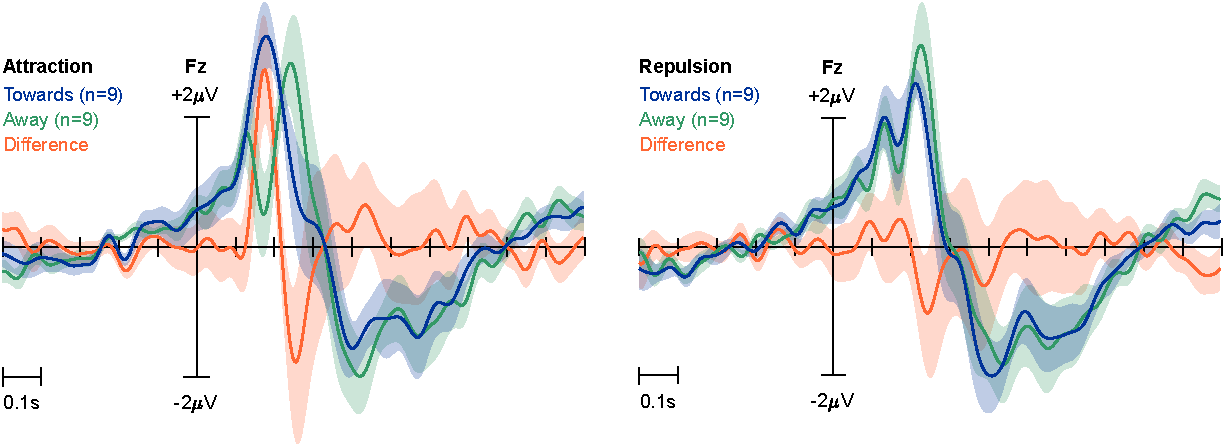
\includegraphics[width=\textwidth]{figures/salval-posfirst-erp-channel.pdf}
    \caption[The grand average ERPs at Fz for the two conditions in the attraction-first group.]{The grand average ERPs at Fz for the two conditions in the attraction-first group.}
    \label{salval:fig:posfirst-erp-channel}
\end{figure}

The repulsion condition (when presented second), however, shows neither the same nor the inverted pattern that would be indicative of salience-only or valence-only processes, respectively, being involved in its production. Rather, at around 180~ms a negative deflection can be seen in both classes. This negativity is smaller than the negativity seen in the attraction condition, with its mean amplitude holding the middle between the attraction condition's negativity and positivity.

Using permutation tests with 10000 permutations, significant differences ($p<0.05$) between the curves are found consistently between 160 and 200~ms in the attraction condition. The repulsion condition shows no significant differences between the two classes, towards and away.

\subsection{Valence- and Salience-Focused Classifier Visualisation}
\label{salval:sec:results:classvis}

Figure~\ref{salval:fig:wdd-within}, discussed above, shows the cortical areas contributing to the first two classifiers from Table~\ref{salval:tab:bci}, which include both salience and valence dimensions. The current study was designed to separate salience and valence, as per the latter four classifiers in Table~\ref{salval:tab:bci}. TvT and AvA both classify visually identical stimuli, but with different meanings, i.e., these classifiers focus on valence, whereas TvA+ and TvA-- both classify visually different stimuli with identical meanings, focusing on visual salience. Because the weighted dipole density plots indicating the contributing cortical areas for the two valence-focused classifiers TvT and AvA are largely similar, we have combined them into one plot, showing the summed distribution of weights for both valence-focused classifiers in the attraction-first group. The same was done for the two salience-focused classifiers. The results are in Figure~\ref{salval:fig:posfirst-wdd-combined-sum}. Figures for the separate classifiers are included in the supplement. 

\begin{figure}[hbtp]
    \centering
    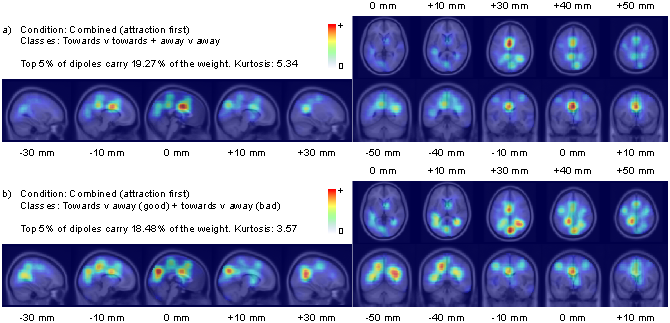
\includegraphics[width=\textwidth]{figures/salval-posfirst-wdd-combined-sum.pdf}
    \caption[Weighted dipole density plots of the combined salience- and valence-focused classifiers, for the attraction-first group.]{Weighted dipole density plots showing the relevance of cortical areas to \emph{a} the two valence-focused classifiers TvT and AvA, and \emph{b} the two salience-focused classifiers TvT+ and TvT--, both for the attraction-first group.}
    \label{salval:fig:posfirst-wdd-combined-sum}
\end{figure}

\clearpage 

Whereas the classifiers which combined valence and salience show three distinct cortical areas contributing to separability, the valence-focused classifiers focus almost exclusively on the mPFC region. The salience-focused classifiers on the other hand, isolate signals from all three regions identified earlier, but focus primarily on the central and lateral parietal regions.


\subsection{The Repulsion-First Group}
\label{salval:sec:results:repulsionfirst}%

Figure~\ref{salval:fig:negfirst-erp-channel} shows the grand-average ERP at Fz for the repulsion-first group. The same effects are visible as in Figure~\ref{salval:fig:posfirst-wdd-combined-sum} of the attraction-first group, albeit less pronounced. Following permutation tests with 10000 permutations, significant differences exist between 164 and 172~ms in the attraction condition. Around that same time in the repulsion condition, both classes show a slight negative deflection, where no significant differences can be reported. Figure~\ref{salval:fig:negfirst-wdd-combined-sum} shows the areas relevant to classification of the valence- and salience-focused activity. Unlike in the attraction-first group, no differences can be reported. Figures for the separate classifiers are included in the supplement.


\section{Discussion}

We presented an adaptation of the original implicit cursor control experiment \cite{zander2014implicit,zander2016nat} which allowed us to separate two dimensions that were originally coupled: salience and valence. Because they were originally coupled, it was unclear to what extent the reported results may have been influenced by perceptual processing of the movements, compared to the participants' valence-related interpretation of each movement. Here, stimuli were kept visually constant across two conditions in which valence was manipulated. This allowed valence processes to be targeted by comparing visually identical stimuli that had different valence, and perceptual (salience) processes to be targeted by comparing visually different stimuli that had the same valence. We hypothesised that, if the primary differences between the classes were to be valence-related, any effect seen within conditions would be inversed between them. Alternatively, there should not be any differences between the conditions if visual processing was the primary generator of such an effect. 

The `effect' in question can be most prominently seen in the ERP at channel Fz. The attraction condition accurately and significantly reproduced the positivity and negativity which indexed the different cursor movements in the original experiment. In the repulsion condition, however, we see neither an inversion nor a reproduction of this effect. Based on this, we can conclude that neither valence nor salience was the sole or primary generator of this particular effect, and indeed further analysis is required to disentangle their respective contributions.

Individually-calibrated classifiers offer a data-driven method to select relevant features from the available data; in our case, the ERPs across all channels between 0 and 600~ms following each cursor movement. The method presented in \citeA{krol2018classvis} allows these features to be localised in the brain, allowing the individual classifiers to be aggregated again across participants in 3D source space. Using this analysis, we see a focused selection of cortical areas that generate the differences between the classification schemes. We focused this analysis on the attraction-first group.

The mPFC was identified in the original experiment as the primary generator and remains prominent here. It points to the involvement of an error monitoring process, as per the reinforcement learning theory \cite{holroyd2002,nieuwenhuis2004rlern}. This is in line with the original interpretation of each movement as `feedback' which can be correct or in error depending on the expectations of the observer, or on the progress that the observer perceives towards the goal.

Since only the grid layout changed between the original experiment and the attraction condition, the increased involvement of the parietal lobe is likely due to the additional perceptual and spatial demands of the adapted grid. It is larger ($7\times7$ instead of the original $4\times4$), and the cursor's movements require additional spatial computation since the relative position of the reference node (the centre) changes more strongly than in the original experiment, where it always remained within one quadrant relative to the cursor. It is this additional computation that likely led to the increased involvement of this area, which is known to be involved in spatial processing \cite<e.g.,>{zipser1988,yantis2002parietalattention,goldberg2006saccadessalienceattention,silk2010spatialwmattention}.

Additionally, both the right-lateral inferior parietal lobule and a combination of the medial frontal and cingulate gyrus were identified by \citeA{dyson2015errorregions} as contributing to erroneous feedback detection, each ranking first, respectively, in two different methods quantifying their contributions. 

From among all the ICs present in the data, the various areas that the different classifiers focused on can thus be reliably related to the task at hand. More interesting is how they relate specifically to the dimensions manipulated in the experiment, and the different functional processes that would be present.

The original assumptions were formulated in the form of predictions or expectations being violated. The valence dimension was manipulated through the instructions, and created a tendency to predict the favourable outcome, i.e. that the cursor would move in the `appropriate' direction. The salience dimension could be interpreted as producing a similar tendency, except that it would preferentially predict that the cursor would move towards the visually salient point regardless of its valence. In this framework, the two predictions are congruent in the attraction condition, with these predictions either both being violated when moving away from the centre, or both being confirmed when moving towards the centre. If each final perception is referenced to both predictions separately and in parallel, with each prediction influencing the dopaminergic input to the mPFC accordingly, this would explain the effects observed at Fz. The congruent violations, each producing a negative deflection, would combine to result in a strong negative deflection as observed, while the strong positivity would reflect the congruent processing of `reward' for the two predictions. In the repulsion condition, the two processes are incongruent; where one would produce a stronger inhibition, the other would disinhibit the mPFC, and vice versa, essentially cancelling each other out. This is in line with the reduced negativities that are pronounced equally in both classes in Figure~\ref{salval:fig:posfirst-erp-channel} for the repulsion condition. 

An alternative account could interpret the negative deflections in the repulsion condition as an N2 component of the ERP, oft-reported to reflect a conflict monitoring process \cite<e.g.,>{nieuwenhuis2003conflictn2,yeung2004}. It largely matches the latency, spatial properties, morphology, and even cortical generators of the feedback negativity, so it cannot be uniquely differentiated from the feedback negativity in the present context---although there are reports that the feedback negativity itself results from conflict monitoring \cite{botvinick2001conflictmonitoring,yeung2004} or is at least sensitive to conflict \cite{jia2007perceptualconflict}. In the current experiment, the presence of a conflict-related process may however be postulated given the experimental design and the reported results. As mentioned above, in the repulsion condition, the salience and valence dimensions are incongruent, i.e., they are in conflict. In the attraction-first group, this may be exacerbated by participants possibly having been primed by the previous condition. Instead of the feedback negativity or reward positivity, a smaller negative deflection is seen reflecting this conflict between either the two predictions mentioned above, or the task parameters more generally. This, too, could explain the ERPs in Figure~\ref{salval:fig:posfirst-erp-channel}. The presence of conflict processing would additionally explain the tendency towards slower reaction times in the repulsion condition, reported for conflict conditions in general \cite{vidal2020errorsactionmonitoring}. 

This latter account, in its simplest form, does not include any effects on the ERP of valence or salience per se in the repulsion condition and focuses merely on conflict. A final account could be a combination of the two above, or the latter account with additional, unspecified processes related to these dimensions. Conflict processing could delay these more specific processes to varying degrees making them difficult to analyse using ERPs. Instead, such processes may be picked up by the classifiers which are individually calibrated and take single-trial variability into account.

Importantly, none of the possible accounts of the data presented above would invalidate the separation of the valence and salience dimensions by the TvT, AvA, TvA+ and TvA-- classifiers as explained in Section~\ref{salval:sec:methods:classification}. If the two processes exist separately in parallel as per the first account, the TvT and AvA classifiers average out the salience violations/confirmations and focus only on valence-related processes, while the TvA+ and TvT-- classifiers do the opposite to focus on salience. In the second account, these cross-condition classifiers would focus on the differences between the relevant process in the attraction condition, and this uniform conflict process. This would not interfere with the conclusion: If indeed the response processing is the same in both classes for the repulsion condition, it would serve as a neutral reference against which to compare the responses in the attraction condition. As such, the concept of salience- and valence-focused classifiers remains valid---although it would introduce additional relevance weights in the region responsible for processing the conflict. Alternatively, if the repulsion condition does additionally have valence/salience processes, or if any combination of the given accounts applies, similarly, a combination of the above two arguments applies and the concept of salience- and valence-focused classifiers remains valid.

We may thus focus on interpreting the differences observed between the classifiers as presented in Figure~\ref{salval:fig:posfirst-wdd-combined-sum}. As mentioned in Section~\ref{salval:sec:results:classvis}, the attraction-first group shows different cortical areas responding to salience and valence. The salience-focused classifier, which in this context should focus on differences with respect to the perceptual (visual) processing of the stimuli, is indeed localised primarily in the parietal areas identified earlier. The additional but weaker mPFC involvement points towards the involvement of either the conflict monitoring process mentioned above in the latter accounts, or the general (prediction) error system whose activity would remain relevant as per the first account.

In line with our hypotheses, the valence-focused classifier carries very little weight in the occipital/parietal regions, and is instead principally focused on the mPFC region, where EEG correlates of both error and reward processing have been postulated to originate \cite{holroyd2008rewardpositivity}, supporting that the feedback-related negativity is indeed at least partially reflective of valence \cite{yeung2004passiveactivefrn}.

The repulsion-first group, however, did not show this same pattern. Here, all classifiers were dominated by the involvement of a larger, less distinct parietal region. This does not rule out that the same patterns do exist in the data---indeed, the other measures do not differentiate this group from the other, and conclusions drawn on the basis of ERP and behavioural analyses apply equally to both groups. The difference in the relevant cortical areas however suggests that this group had a fundamentally different approach to the tasks in both conditions. It appears that the two conditions here cannot effectively be counter-balanced as intended, instead resulting in what are essentially two different experiments. Still, as a last validation, Figure~\ref{salval:fig:allparticipants-wdd-combined-sum} shows the valence- and salience-focused classifier localisation as applied to the data for both groups together. The conclusion as mentioned above with respect to the differential involvement of parietal and prefrontal cortical areas can still be drawn, with the different classifiers predominantly focusing on different areas. In the combined data, however, we also see the consistent involvement of an additional parietal area in both classifiers, an area which we now know to be explained by its exclusive presence in the repulsion-first group. As such, the separation of the two groups in this analysis helped sharpen the results. It also highlighted the importance of investigating the cortical origins of classifiers, a step which is often omitted.

We have shown that both salience and valence, i.e., both the visual properties of the presented stimuli as well as the subjective interpretation of these stimuli, play a role in the implicit cursor control paradigm as presented here and used before \cite{zander2014implicit,zander2016nat}. Furthermore, classification schemes can be developed to focus primarily on one or the other aspect. The differential processing of these aspects is supported by their different cortical origins.

Now taking a wider perspective, we wish to come back to the implications of the present results for neuroadaptive technology. The unit of analysis in this paper was the individual cursor movement, which was classified on single-trial basis. Single-trial classification allows the classifier output to be used in real time as input to a computer, e.g., to enable control. This control can be implicit if the brain activity that is being classified is not consciously or voluntarily modulated by the human. Implicit cursor control is an interesting case in that it demonstrates that the task of moving a cursor, which is a quintessential example of explicit control, can in fact be performed implicitly without participants being aware of doing so \cite{zander2014implicit,zander2016nat}: indeed there was no conscious or voluntary manipulation of brain activity that helped steer the cursor. When control or interaction happens unbeknownst to the users themselves---the ones supposed to be in control---the exact cognitive and affective processes that a classifier can potentially access make a profound difference with respect to the forms of interaction and the types of application that can be realised. The current results support the position that classifiers can access both perceptual processes, potentially allowing brain-as-a-sensor applications to be developed, and valence-related processing, i.e. cognitive processes that reveal subjective value judgements of the users. This latter category enables, among other things, unique forms of personalisation that may greatly increase productivity, but, given the deeply personal nature of the brain activity, may at the same time introduce particularly severe issues with respect to privacy \cite{mecacci2019criteria}, data security \cite{fairclough2014confidential}, informed consent, and outcome responsibility \cite{krol2020cognitiveprobing}. While we are looking forward to the further exploration of the possibilities of neuroadaptive technology, the current results emphasise that researchers and developers should take these potential issues into account. 


\section*{Acknowledgements}

Part of this work was supported by the Deutsche Forschungsgemeinschaft (ZA 821/3-1). 


\section*{References}

A shared bibliography starts at page~\pageref{bibliography}.

\vfill

\begin{figure}[!h]
    \centering
    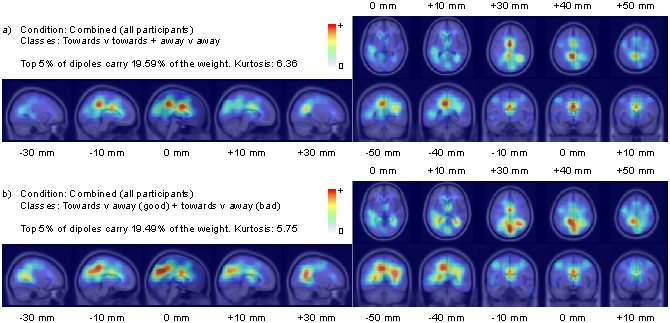
\includegraphics[width=\textwidth]{figures/salval-allparticipants-wdd-combined-sum.pdf}
    \caption[Weighted dipole density plots of the combined salience- and valence-focused classifiers, for all participants combined.]{Weighted dipole density plots showing the relevance of cortical areas to \emph{a} the two valence-focused classifiers TvT and AvA, and \emph{b} the two salience-focused classifiers TvT+ and TvT--, for all participants, i.e. combining both attraction-first and repulsion-first groups.}
    \label{salval:fig:allparticipants-wdd-combined-sum}
\end{figure}

\vfill\null

\clearpage
\begin{figure}[t]
    \centering
    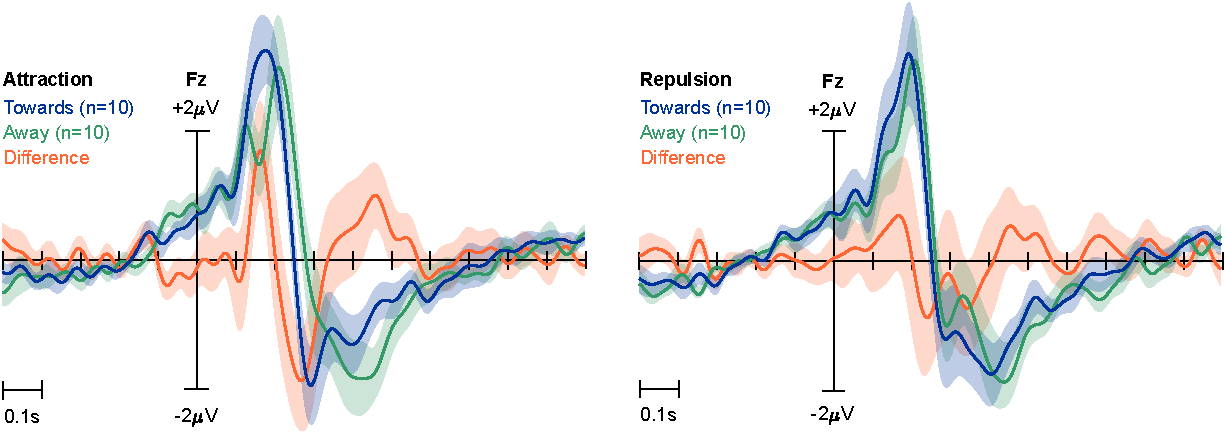
\includegraphics[width=\textwidth]{figures/salval-negfirst-erp-channel.pdf}
    \caption[The grand-average ERPs at Fz for the two conditions in the repulsion-first group.]{The grand-average ERPs at Fz for the two conditions in the repulsion-first group.}
    \label{salval:fig:negfirst-erp-channel}
\end{figure}

\begin{figure}[b]
    \centering
    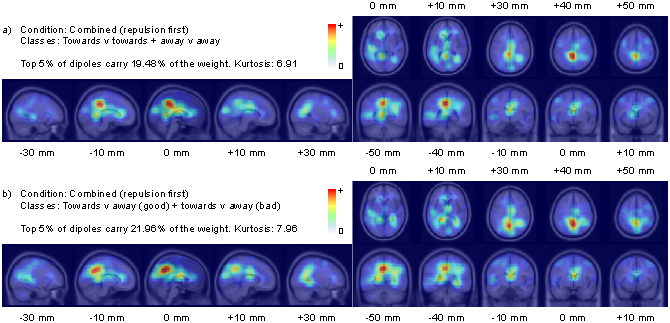
\includegraphics[width=\textwidth]{figures/salval-negfirst-wdd-combined-sum.pdf}
    \caption[Weighted dipole density plots of the combined salience- and valence-focused classifiers, for the repulsion-first group.]{Weighted dipole density plots showing the relevance of cortical areas to \emph{a} the two valence-focused classifiers TvT and AvA, and \emph{b} the two salience-focused classifiers TvA+ and TvA--, both for the repulsion-first group.}
    \label{salval:fig:negfirst-wdd-combined-sum}
\end{figure}




\clearpage
\pagestyle{empty}
\null\cleardoublepage
\pagestyle{plain}

    
    \bookmarksetup{startatroot}
    \addtocontents{toc}{\bigskip}
    
    \cleardoublepage%
\phantomsection\addcontentsline{toc}{chapter}{Discussion}%
\chapter*{Discussion}

Three quotes were used to introduce this dissertation, all of which bear some relevance to the topic of neuroadaptive technology. As we have seen, neuroadaptive technology uses implicit input obtained from brain activity in order to adapt itself, e.g. to enable control or interaction, with implicit input referring to any actionable input to a system that was not intended as such by its source (cf. \citeNP{schmidt2000}). A quote from \citeApos{byrom1976dhammapada} admittedly liberal rendering of Chapter~I, Verse~1 of the Dhammapada, `With our thoughts, we make the world', may take on a new meaning in the context of implicitly brain-actuated environments. Although this is most probably not what the Buddha had in mind, an abstractly-formulated vision of neuroadaptive technology is to essentially allow our free thoughts to interact with the world unhindered, shaping it through continuous adaptations to the benefit of those persons whose thoughts have made it so. This may sound like a highly indulgent description of the matter, but at its core---unforced mental states adapt the external context to better support the human---it does embody the main benefits offered by even the most limited of today's laboratory demonstrations of neuroadaptive technology, let alone the applications envisioned for the future.

One necessary requirement for these benefits to be realised, is that our `thoughts' do indeed enter `the world' in some form, i.e. our brain activity must be externally monitored and decoded. This would add to the body of personal data that is already being gathered about virtually all users of modern technology. There exist multiple potential stakeholders to such data, including stakeholders like Edward Bernays, the late pioneer of using psychological insights to manipulate society to the benefit of paying customers, i.e., of propaganda. We should remain vigilant that additional insight into the `mental processes and social patterns of the masses' \cite{bernays1928propaganda}, which commercial neuroadaptive technology may enable to be gathered at scale and in real time, is not used against the public interest.

This is all the more pertinent in cases where the user may not be able to prevent information from being gathered in the first place. The concept of cognitive probing gives the computer some autonomy over the process of information gathering, and it has not yet been established that a user can counteract the automatic informative responses that are elicited by cognitive or affective probes. It is of such scenarios that the third quote serves to remind us, on page~\pageref{quote:locutus}.

These concerns may not appear to be immediately relevant today. It is true that many of the scenarios used to illustrate both potential benefits and potential adverse effects of neuroadaptive technology are based on speculation: for example, speculation concerning the general availability and adoption of brain monitoring hardware, speculation concerning the real-world accuracy of mental state classifiers, and speculation concerning our future living and working environments. Even this very dissertation introduced the topic with a speculative example of a neuroadaptive book. However, we are now in a position to make the same arguments without reference to thought experiments or science fiction. As also stated in the introduction, it is the main argument of this dissertation that neuroadaptive technology has now sufficiently progressed to warrant both widespread interest and widespread concern. A range of possible beneficial applications, as well as a number of important concerns regarding the use of neuroadaptive technology have been presented in Part~\ref{part:concepts} of this document. Subsequently, using tools and methodology developed in Part~\ref{part:tools}, two validations presented in Part~\ref{part:validations} demonstrate a number of key facts.

Specifically, Chapter~\ref{chapter:pbci} looked at existing passive BCI research and applications, and used a novel categorisation to identify a current trend \cite{krol2018interactivity}. It found that four different degrees of interactivity can be distinguished, starting with the theoretical zero-point which is required for pBCI to work: the ability in and of itself to assess mental states from recorded brain activity. Research is ongoing to produce and validate more accurate feature extraction and classification algorithms \cite<e.g.,>{lawhern2018eegnet,mousavi2019error,xu2020tangentriemannian} to improve and expand the computer's ability to decode our mental states, but a good number of proven methods already exist \cite{lotte2018classificationreview}. These methods can also be used in real time, allowing the computer to respond to the detected mental states. This makes the computer interactive, and enables it to adapt to the received implicit input---i.e, it enables neuroadaptive technology. The first interactive category includes open-loop systems, which adapt to the detection of pre-determined mental states in a pre-determined way. For example, the detection of a mental state reflecting the user's intention to interact with an object, as investigated by \citeA{protzak2013gazebased} and \citeA{shishkin2016wishmouse}, could be used to replace explicit control instructions such as button presses. The second interactive category deals with closed-loop neuroadaptive systems, in which the adaptations performed by the computer have an influence on the mental states that triggered the adaptation in the first place. In such closed-loop settings, neuroadaptive systems may for example detect workload levels and aim to bring them into balance \cite{kohlmorgen2007,afergan2014dynamicdifficulty}, or neuroadaptive learning environments can pace the learning experience to optimise student engagement \cite{yuksel2016bach,walter2017adaptivelearning}. The final category deals with automated adaptation, also known as intelligent adaptation \cite{fairclough2017intadapt}. Here, the computer employs a user model in which it stores the mental states it has decoded alongside the situational parameters in which they occurred, giving it a database from which to infer higher-order relations and causal effects. This concept has been used extensively by non-passive BCI systems aimed at explicit communication and control (see e.g. \citeNP{rezeika2018bcispellerreview} for a review), but a number of unique opportunities are created when it is employed by pBCI systems. Of particular interest is the fact that systems from this final category may have the ability to autonomously gather additional information needed to make more reliable inferences. The method that makes this possible, called cognitive probing, was discussed in more detail in Chapter~\ref{chapter:cp} and a demonstration was presented in Chapter~\ref{chapter:nat}.

Chapter~\ref{chapter:cp} explained in detail how neuroadaptive technology can use cognitive probing to obtain specific pieces of information. The newly-defined concept rests on the understanding that certain events automatically evoke responses from us. For example, it is virtually impossible not to read a word that is visually presented to us, and once we have read it, we have its semantic concept in mind. Also on a higher level, many cognitive and affective processes are beyond our conscious control: seeing or hearing something we like automatically brightens our mood, even if ever so slightly. These automatic responses are reflected in our brain activity. A system that has access to this brain activity, and the ability to interpret the appropriate mental states, could make use of this by presenting us with various stimuli and gauging our brain's automatic responses to them. One important reason why a system may want to do this is to update its user model. This model mentioned in the previous paragraph, where a user's mental state is recorded as a function of situational factors, may be incomplete, leaving the computer unable to infer information with the desired level of confidence. Cognitive probes can then be used to elicit the missing responses from the user, which are then stored in the model to fill in the gaps. As such, this method allows neuroadaptive systems to autonomously gather information from brain activity they deliberately induce in their users. A cognitive probe was defined as `a technological state change that is initiated or manipulated by the same technology that uses it to learn from the user's implicit, situational, cognitive or affective brain response to it' \cite{krol2020cognitiveprobing}. There is a steadily increasing number of examples in the literature that use various independently developed implementations of this method, which the provided definitions now allows to be recognised as sharing a fundamental similarity \cite<e.g.,>{dalseno2010,peck2013brainrecommender,iturrate2015teaching,kirchner2016multirobotcontrol,lorenz2016automaticneuroscientist,mladenovic2019activeinference}. Recognising the shared foundations of these previously separate approaches also allows a generic framework to be built in which both the benefits and the potential risks of the method can be described and analysed. The main benefit of implicit input itself is clear: it allows meaningful communication to take place without requiring any explicit instructions to be formulated. With cognitive probes specifically eliciting implicit input, the technology does not have to wait for the human to (implicitly) initiate the communication, but can autonomously gather the information it needs to best support the human. Furthermore, to the extent that it can target automatic responses, cognitive probing may be capable of obtaining information that could not be gotten any other way---not even by asking someone directly. As for the risks, importantly, cognitive probing requires the computer to have some autonomy in deciding what to present to the user, meaning it must also have its own logical reasoning to make these decisions. In other words, the computer can be seen to have its own \emph{agenda} \cite{fairclough2017intadapt} which may not necessarily align with the user's. With an adverse agenda, such a system may be able to extract responses from users against their will---to the extent that they are automatic---or induce undesirable mental states. Chapter~\ref{chapter:cp} therefore also discussed a number of technical aspects to consider, as well as ethical aspects concerning consent, privacy, agency, and responsibility. Care must be taken that autonomously operating systems with the ability to elicit and access implicit brain responses handle their influence and the obtained data with due care for their users.

The concepts and systems described in Chapters \ref{chapter:pbci} and \ref{chapter:cp} rely on real-time access to cognitive and affective states, decoded from a continuous recording of brain activity. The range of possible applications, as well as the severity of some of the ethical concerns surrounding these systems, thus depend on the exact types of cognitive and affective states that can be reliably detected. This is commonly determined through clever experimental designs aimed at uniquely eliciting specific mental states, but it is important to be able to verify these claims on the basis of the recorded data, and to make sure that the classifiers do in fact target the intended mental states. Chapters \ref{chapter:sereega} and \ref{chapter:visualisation}, therefore, introduced new tools to validate some of the analysis and classification methods that are in common use today.

Chapter~\ref{chapter:sereega} presented SEREEGA, a toolbox to simulate event-related EEG activity. It allows a signal comparable to the one normally recorded by real EEG electrodes to be produced from the ground up: a user of the toolbox can configure the exact parameters of the desired cortical processes, which will then be simulated to produce realistic scalp-level time series. The underlying parameters thus constitute a known ground truth describing the simulated processes. This is important, as such a ground truth is not available for real EEG recordings. Many EEG analysis techniques exist to attempt to uncover these `parameters' of real recordings, including the event-related potential technique to find true activation patterns in spite of noise and variability \cite{luck2014erp} and independent component analysis to find the cortical sources of the activations \cite{makeig1996}, and many more continue to be developed. To evaluate the efficacy and accuracy of these methods, however, a ground truth is needed to compare their results to. Therefore, researchers and developers often turn to simulations. Even though simulation has long been a popular method, no standardised toolbox existed for this purpose until the publication of SEREEGA \cite{krol2018sereega}. SEREEGA's functionality covers and extends the vast majority of past and present EEG simulation approaches, and the toolbox's architecture and open-source licence allows it to be readily extended with additional features. It makes EEG data simulation more accessible, standardised, and reproducible. 

SEREEGA-simulated data was used in Chapter~\ref{chapter:visualisation} to validate a classifier visualisation method. In data-driven approaches to BCI, machine learning is employed to select relevant features from the recorded data. These features are selected based on their utility to distinguish between the classes under investigation. In a way, achieving significant classification accuracy thus means that features can be identified that allow the classes to be reliably distinguished from each other. Importantly, however, in and of itself, a significant classification accuracy does not mean that the features selected by the classifier bear any relevance to the cortical processes that were intended to be targeted. If non-cortical activity is present in the data, which is almost always the case in raw EEG recordings, a classifier will make use of this activity whenever it aids the separability of the classes. For example, eye blinks and muscle activity often correlate to various task parameters. Such activity can thus be very informative, but may be liable to be influenced by irrelevant parameters as well: eye blinks, for example, may change as a function of environmental humidity. Therefore, it may be preferable to target cortical activity specifically. The method presented in Chapter~\ref{chapter:visualisation} visualises the areas that an EEG-based spatio-temporal classifier focuses on, allowing the different sources to be spatially separated, identified as cortical or non-cortical, and neurophysiologically interpreted. It does this by first transforming the classifier's filter weights into patterns \cite{haufe2014}, representing the projection of the areas isolated by the classifier onto the scalp (i.e., the forward model). These can then be decomposed into contributions from individual sources using a separately obtained unmixing matrix from blind source separation methods such as independent component analysis. This decomposition then assigns a so-called relevance weight to each source. Since the sources can be localised in 3D space, so can these relevance weights be assigned to a location. Using a 3D weighted kernel density plot, the weights can then be visualised in a virtual brain to identify which areas contributed to classification. This not only allows us to evaluate to what extent a classifier focused on cortical as opposed to non-cortical sources, it also provides insight into \emph{which} cortical areas, exactly, contribute to classification. With this method, we can thus even use classification methods to expand our understanding of the functional processes in the brain, introducing classifier-based neurophysiological analysis to neuroscientific research in general.

The tools introduced in Chapters \ref{chapter:sereega} and \ref{chapter:visualisation}, then, enabled us to validate the concepts introduced in Chapters \ref{chapter:pbci} and \ref{chapter:cp}---in particular, the notion of implicit control based on automatic brain responses elicited by cognitive probes.

The experiment described in Chapter~\ref{chapter:nat} demonstrated implicit control over a cursor. It consisted of two phases. In a first calibration phase, participants were shown a cursor moving randomly over the nodes of a $4\times4$ grid, with one of the corners indicated as the target. Participants were instructed to judge each individual cursor movement as either `appropriate' or `inappropriate' with respect to the larger goal of reaching the indicated target. A classifier was then trained on EEG data gathered in this first phase, separating `appropriate' from `inappropriate' movements with a mean estimated average accuracy of 72\% across participants. In a second online phase, this classifier was used to reinforce the cursor in real time. Initially, the cursor moved randomly: each cursor movement served as a cognitive probe, eliciting a response from the observing participant that served to categorise that movement as either appropriate or not. Based on that information, the model that reflected the participant's preferences with respect to the cursor movements was adjusted. Since the cursor's movements were based on this same model, the cursor came to behave increasingly in line with these preferences, even as the participants were unaware of causing any changes. As such, this online reinforcement based on implicit input led to significantly goal-oriented behaviour of the cursor, i.e., implicit cursor control. The classifier visualisation methods described in Chapter~\ref{chapter:visualisation} revealed that the classifier focused almost exclusively on the medial prefrontal cortex to extract the implicit input in question, supporting the interpretation that the underlying cortical processes are indeed automatic brain responses: they most likely relate to predictive coding, a fundamental process in which our brains continuously predict future (neuronal) events and compare those predictions to the actual final occurrences in order to optimise our behaviour. Such a fundamental process is unlikely to be under direct conscious influence, while at the same time, Chapter~\ref{chapter:nat} concluded, it can reflect higher-order cognition: in this case, it reflected fine-grained preferences with respect to cursor movements. Where traditional human-computer communication is restricted by the speed and accuracy with which humans can provide explicit instructions, this demonstration of effective cursor control through implicit interaction thus illustrated how neuroadaptive technology can bypass these limitations, effectively widening the communication bottleneck and decreasing the asymmetry present in current human-computer interaction paradigms.

In this demonstration of implicit cursor control, the classifier visualisation method was used to analyse which cortical processes significantly contributed to classification, and to support the conclusion that the used input was indeed implicit. However, it could not be determined with certainty that the targeted cortical activity was primarily informed by the participants' subjective preferences, as assumed, and not by more `neutral' cognitive processes such as those related to visual processing of the stimuli. For a deeper look at the processes underlying the implicit cursor control paradigm, Chapter~\ref{chapter:salval} therefore presented an adapted paradigm allowing two particular dimensions to be separated: visual salience and valence. The grid was larger, the corner nodes were removed, and a visually highlighted reference node was placed at the centre of the grid. As before, a cursor could move across the nodes of this grid. In two separate conditions, these visual (salience-related) aspects of the experimental paradigm were left constant, while the subjective (valence-related) interpretations of the cursor's movements were manipulated through the instructions: a movement towards the centre was `appropriate' in one condition, but `inappropriate' in the other. This allowed different classifiers to be calibrated focusing either on salience or on valence. The results of this analysis indicated that both salience and valence play a role during implicit cursor control as separate processes. Using the visualisation method from Chapter~\ref{chapter:visualisation}, we could reveal that the different classifiers could reliably isolate salience and valence from different cortical areas. Although this was certainly not the first experiment isolating valence-related activity from EEG, this experiment did demonstrate its presence in the implicit cursor control paradigm, and illustrate the utility of localising classifier weights in 3D source space for both BCI applications and neuroscientific research in general.

Furthermore, the fact that neuroadaptive technology can isolate and interpret brain activity indicative of subjective valence has important implications, concerning both the range of potential neuroadaptive applications, and the potential ethical issues that may arise from such applications. The results of these latter two chapters thus demonstrated the concepts described in Chapters \ref{chapter:pbci} and \ref{chapter:cp} as well as their potential benefits, but also validated the concerns addressed in those chapters. An important question thus remains: Going forward, as a field, how can we weigh what is possible against what is desirable?


\phantomsection\addcontentsline{toc}{section}{Value-Guided Research}%
\section*{Value-Guided Research}%

Already in 1980, Collingridge considered `one of the most pressing problems of our time: can we control our technology---can we get it to do what we want, and can we avoid its unwelcome consequences?' In this consideration, the avoidance of unwelcome consequences is the domain of governmental policies placing limitations and controls on the technology, determining what is allowed in what form. The problem in deciding this, however, is twofold. When a new technology is still in its infancy, its potential unwelcome consequences cannot be predicted with sufficient accuracy to justify any hard, legal limitations on its use. Given the unpredictable but inevitable and sweeping interactions that happen between technology and society, however, it is as good as certain that unwelcome consequences will arise at some point, but when these consequences finally surface, the technology has become so pervasive as to make limitations and controls difficult and expensive to implement. In Collingridge's words:

\begin{quote}
    This is the \emph{dilemma of control}. When change is easy, the need for it cannot be foreseen; when the need for change is apparent, change has become expensive, difficult and time consuming.
\end{quote}

This dilemma is now referred to as the Collingridge dilemma. \citeA{collingridge1980socialcontrol} illustrated it in the context of techno-societal issues such as the toxicity of lead in petrol, nuclear power plants, the Manhattan Project, and other forms of weapons research. We can see how it currently also applies to consumer neurotechnology in general, and neuroadaptive technology in particular. With commercial applications of neurotechnology now being marketed directly to consumers, but not yet having reached a point where other technologies, economic institutions, or social conventions rely on it, it would be minimally disruptive to limit or control the market at this point. At the same time, there is no pressing, justifiable reason for it: no harm is currently being done, clear potential benefits have been identified, and corporations big and small have explicitly shown interest in the technology. 

The precautionary principle is often suggested as a solution to this dilemma, essentially disallowing the technology until its safety has been proven. This principle is already employed by some regulatory bodies of the European Union, especially as regards the environment. A criticism of this approach, however, is that it stifles innovation. When dealing with the uncertainties of a technology's future influence on society, Collingridge instead proposes a method of decision making that recognises that the debate is essentially about values, but nonetheless focuses exclusively on facts. From his example of lead in petrol, a generally-accepted value $V_1$ may be formulated as \emph{If X eliminates a health hazard, X ought to be done}. Combined, then, with the fact $F_1$ that \emph{Reducing the amount of lead in petrol would eliminate a health hazard}, their conjunction $F_1 \land V_1$ leads to the conclusion $V_2$ that \emph{The amount of lead in petrol ought to be reduced}. The argument thus begins and ends with value statements, but hinges on $F_1$. Collingridge emphasises that, rather than debating values directly, a set of shared initial values allows the debate to focus on facts, allowing it to be argued on the basis of hard data. The environmental protection agency and the petro-fuel additive manufacturer never disagreed on $V_1$, instead arguing the evidence for and against $F_1$, using any number of additional facts.

This model could provide some structure to the ongoing discussion regarding potential ethical, legal, and societal implications of neuroadaptive technology. It suggests that we separate values from facts, and that a constructive step may be to find a set of relevant common values. 

A lot has been written about values relevant to neuroadaptive technology; in some cases, this is already in the form of clearly formulated values, in others, it is a broader analysis of how neuroadaptivity relates to a particular set of values. On many issues, however, which themselves are widely recognised as valid issues, no shared consensus has been reached. \citeA{fairclough2014confidential}, for example, argues that any physiological data must be treated with the same confidentiality as medical data, stating that `that is what they are'. \citeA{kellmeyer2018bigbraindata}, on the other hand, points out that there is no generally accepted definition of biomedical data that would presently allow us to classify brain data as such: as an analogy, he points out that medically-relevant information has been inferred even from supposedly non-medical sources of data such as text messages and a smart phone's location data. If brain activity is medical data because medical conclusions can potentially be drawn from it, should text messages be medical data too? This discussion, however, in part mixes values and facts. Both authors implicitly agree that \emph{personal data should be protected}, and that \emph{medical data should have higher standards of protection than personal data}. They furthermore agree with the fact that \emph{neurotechnology processes brain data} and that \emph{brain data is personal data}; they disagree, however, whether \emph{brain activity is medical data}. The Collingridge perspective thus focuses the debate on this latter fact, and suggests that new research should be conducted to support or contest this issue in particular, rather than continuing to discuss which values ought to apply.

Similarly, proponents of cognitive liberty argue that no individual may be compelled against their will to use neurotechnology, nor that they should be prohibited from doing so, as long as no harm befalls others \cite{boire2000cognitiveliberty}. They propose this as a necessary extension to the freedom of thought, stating that `the right and freedom to control one's own consciousness and electrochemical thought process is the necessary substrate for just about every other freedom' \cite{sententia2004cognitiveliberty}. Neuroadaptive technology, especially when using cognitive probing as described in Chapter~\ref{chapter:cp} \cite{krol2020cognitiveprobing}, may in fact interfere with such freedom in ways that are not clearly covered by the current concept of cognitive liberty, which assumes that the human controls the technology. If someone voluntarily chooses to use neuroadaptive technology, but this technology then uses implicit input to influence their mental states without this person's awareness---potentially even against their interests---to what extent, exactly, is this person free to choose their use of the technology? To what extent are they in control of the outcome when the outcome is produced from their implicit input? And by extension, who would bear responsibility for such an outcome? For example, the implicit cursor control experiment was designed to guide the cursor towards the intended target. Using the exact same input, however, it could also be inferred where the user did \emph{not} want the cursor to go---and the cursor could be steered there instead. The same data can be used both to support the user, and to generate the exact opposite outcome.
% while the reader of the neuroadaptive book, encountered in the introduction to this dissertation, may wish to read a happy story, the book itself can use the exact same input to instead generate the opposite of what the reader desires.
And even when the outcome is seemingly favourable, `although [humans] may be certain about what they wanted, they may be insecure about whether they did or did not ``do'' it, and even wrong about what they think they wanted' \cite{haselager2013agency}. 

This points to a deeper issue that may boil down to the definition of `control'. What does it mean, exactly, for someone to be in control of the neurotechnology they use? Fields such as control theory, also applied to human-computer interaction, consider this question to be exclusively confined to the realm of facts; for example, they assign `control' a fixed definition based solely on the mechanical or logical functioning of the technology \cite<e.g.,>{ieeedictionary}. However, neurotechnology allows humanity and technology to become increasingly interwoven, making a reliance only on the technological aspects seem one-sided. As we have seen, e.g. in Chapters \ref{chapter:pbci} and \ref{chapter:cp}, and in \citeauthor{haselager2013agency}'s comment concluding the previous paragraph, in a neuroadaptive interplay between user and technology it may no longer be as clear who does what, or who controls whom. In light of considerations to separate facts and values, it may therefore actually be worthwhile to consider control, as in `being in control', to be a value instead---a value that is yet to be defined and agreed upon. As a value statement, as opposed to a fact, a notion of `control' can give due consideration to ethical issues surrounding the use of technology. For example, it could allow a reader to be formally considered to implicitly control a neuroadaptive book if and only if the actions performed by the book are consonant with the reader's immediate wishes. Such a value statement can then be combined with facts pertaining to various neuroadaptive control mechanisms to ascertain whether a particular application does or does not enable `control', and by extension, whether the human is a `user' or not. This is of crucial importance to interpret statements, such as those referring to cognitive liberty, with respect to the freedom to \emph{use} neurotechnology and to \emph{control} one's consciousness. 

This additional perspective on Collingridge's original method thus forces us not to simply list known values and facts, but also to consider more closely whether some facts perhaps ought to be seen as values, and vice versa.

The explicit consideration of societal values also widens the perspective beyond issues concerning the immediate context of the technology and its individual user. The adoption of new technology by a society is unlikely to progress uniformly, and may affect different people in different ways. BCI research oriented at explicit communication and control applications has found that roughly 20\% of participants are not able to reliably generate a detectable control signal, in some cases simply because of the anatomical structure of their brains, which cannot be changed \cite{allison2010illiteracy}. It is unknown to what extent this may affect the various passive measures of cognition which form the basis of neuroadaptive technology, but it should be assumed that, for any given neurotechnology, a part of the population may simply not be able to use it. Conversely, when states can accurately be detected, there may be a part of the population for whom these states more often constitute invalid or counter-productive information than for others---people suffering from post-traumatic stress or obsessive-compulsive disorders, for example, may not be able to benefit from closed-loop neuroadaptive systems in the same way as others. Such considerations apply to all new technologies, of course, but their applicability to neuroadaptive technology may not be as predictable as for other technologies, which generally rely on explicit interaction.

It might thus be of interest to organise a series of workshops where a list of values may be gathered and discussed: a documentation of values that are relevant to neuroadaptive technology, the extent to which they are currently contested, and what facts would be required to either adhere to or conflict with them. Such a document could be more actionable than e.g. the list of four priorities that resulted from an earlier more general workshop \cite{yuste2017ethical}, as it would generate research questions with respect to facts that are either currently disputed, or currently unknown but bear direct relevance to the identified values. Accepting, for example, that the privacy of thought ought not to be violated, one can then design research to attempt to elucidate at what point any particular neuroadaptive application does indeed violate the privacy of thought \cite<e.g.,>{haselager2018reading}, and to investigate what may be done to protect it. Of particular impact, then, will be research producing new facts that demonstrate an application's incompatibility with society's fundamental values: such facts, combined with an authoritative list of said values, must lead to regulatory action, as per Collingridge's original model. Being guided by values, we may thus discover the vast benefits that neuroadaptive technology can offer society, by striving first and foremost to discover and demonstrate those forms of neuroadaptive technology that ought not to exist.


\phantomsection\addcontentsline{toc}{section}{In Conclusion}%
\section*{In Conclusion}%

The chapters of this dissertation presented conceptual, methodological, and experimental advances in the field of neuroadaptive technology. Part~\ref{part:concepts} provided conceptual frameworks to unify previous works and guide future research. Part~\ref{part:tools} presented new tools to help validate some of the technology's core methods. Part~\ref{part:validations}, finally, experimentally demonstrated a number of key possibilities. 

Honestly admitted, there is an inherent danger in mass-processing personal data, especially where it concerns uniquely sensitive, involuntarily produced brain data. Openly discussed, however, there is no need for the potential risks to outweigh the potential benefits. Properly guided, neuroadaptive technology may lead to environments where, through completely new notions of `interaction', our thoughts really do make the world.

    
    \addtocontents{toc}{\bigskip}
    
    \cleardoublepage\phantomsection\label{bibliography}
    \bibliography{bibliography}
    
    \listoffigures
    \listoftables
    
    
\chapter*{Chapter \ref{chapter:nat} Supplementary Information}
\chaptermark{Chapter \ref{chapter:nat} Supplementary Information}
\addcontentsline{toc}{chapter}{Chapter \ref{chapter:nat} Supplementary Information}

\noindent\emph{Note: The `main manuscript' referenced in this supplement refers to Chapter~\ref{chapter:nat}. As such, `figure 1 of the main manuscript', for example, refers to figure \ref{chapter:nat}.1.}


\section*{Materials and Methods}


\subsection*{Experimental Setup}

Two computers were used for this experiment: One to display the stimuli and another to record EEG. Stimuli were shown on an Iiyama ProLite B2776HDS 27$''$ display using a resolution of 1920$\times$1080 pixels, located approximately one meter away from the participants. The keyboard used was a standard US layout computer keyboard.

EEG was recorded continuously using 64 active Ag/AgCl electrodes (actiCAP; Brain Products GmbH, Munich) mounted according to the extended 10-20 system on an elastic cap (EASYCAP GmbH, Munich). The signal was sampled at 500 Hz and amplified using BrainAmp DC amplifiers (Brain Products GmbH, Munich). All electrodes were referenced to FCz and the ground electrode was placed at AFz.

EEG data was recorded and combined with the paradigm's markers using the Lab Streaming Layer framework (Swartz Center for Computational Neuroscience [SCCN], University of California, San Diego [UCSD]).


\subsection*{Experimental Paradigm}

The cursor's movements were restricted by the nodes of a visible grid. The cursor started out on one of these nodes and, for each movement, could only move to one of the adjacent nodes. Depending on the cursor's position in the grid, then, there were up to eight possibilities for one movement. The grid consisted of gray open circles connected by gray lines on a black background. The cursor in this paradigm was a red, filled circle. The cursor's size was 4.5\% of the display's total height, the grid nodes' size 6\%, and the horizontal and vertical grid lines' length 15\%. Line thickness between the grid nodes was set to 2 pixels. `Red' was pure \textsc{RGB}(255,0,0), `gray' \textsc{RGB}(51,51,51) and `black' \textsc{RGB}(0,0,0). The dimensions of the grid are discussed below.

An animation allowed the participants to be able to anticipate the moment of each movement. Over the course of one second, a white `ghost cursor' would grow inside of the actual cursor. As soon as this ghost reached the same size as the actual cursor, it would instantaneously be repositioned to the chosen adjacent node, while also highlighting the grid line connecting the two nodes in white. `White' here was pure \textsc{RGB}(255,255,255), and the highlighted grid line's thickness was increased to 3 pixels. The movement remained visible for one second, with the red original cursor still on the initial node, the white ghost cursor on the new node, and a white line connecting them. Following that, all whites disappeared and the (red) cursor would instantaneously move to and remain at its new position, on the new node, for another second, before the animation would start over for the next movement. In all, a single trial was three seconds in length.

Grids of three different dimensions were used in this study: One by three nodes ($1\times3$), four by four nodes ($4\times4$), and six by six nodes ($6\times6$).

On each grid, a single red node in one of the corners indicated the current target. Once the cursor had landed on this target node, a new grid was started with the same dimensions, but a different layout. For the $1\times3$ grids, each new grid was rotated either 45, 90, or 135 degrees relative to its predecessor, and a new target corner was chosen at random (`corner' here is one of the two ending nodes of the grid row). The larger grids did not rotate, but a new target was selected for each new grid such that no two subsequent grids had a target in the same corner. Each newly started grid was displayed for one second before the first movement was initiated, for the participants to orient themselves.

In all grids, the cursor's starting position was one node away from the corner opposite the target's, in a straight line to the target. 

Supplementary Figure S1 illustrates the stimuli; Supplementary Movie S4 contains animated stimuli as seen by the participant.

For each individual cursor movement, a movement direction was chosen randomly from the set of possible movements. By default, all possible directions had an equal probability of being selected, and during the offline (calibration) sessions, these initial probabilities remained unchanged---the cursor was unbiased and moved randomly. However, during online application of the pBCI, the directional probabilities were altered based on the classification of each movement as either `correct' or `incorrect', biasing the cursor to repeat movements classified as `correct'.

Specifically, all movement directions were represented a specific number of times in the set from which each new movement was randomly selected. After classification, the respective directions' numbers were increased or decreased such that the resulting probability of each subsequent direction is given by

\begin{displaymath}
    p=\frac{mx}{n+(m-1)x}
\end{displaymath}

\noindent where $x$ is the respective direction's initial number of shares in the set, $n$ is the full set's initial size, and $m$ is a multiplier. For a movement classified as `correct', $m$ was 2.0 for that movement's direction and 1.5 for the two adjacent directions; for movements classified as `incorrect', $m$ was 0.5 and 0.75, respectively. All directions started with a share of 100 elements each in the set. All shares below 1 were rounded up at the time of selection.

The adaptation of adjacent directions represents a certain degree of leniency which the participants were assumed to show in their judgements: If the target is a few nodes north of the cursor's current position, a first move to the north-west is imperfect but may still be acceptable. Therefore, the feedback received from a movement to the north-west should not only alter this specific direction's probability, but should also influence subsequent movements to both the north and the west. 

All visible on-screen events were marked in the EEG stream and additional information about each cursor movement was logged, including distance to the target and the movement's direction relative to the target direction (i.e., a straight line unconstrained by the grid represented a 0$^\circ$ movement).

The paradigm was written in Python using the Simulation and Neuroscience Application Platform 1.02-beta (SCCN, UCSD; https://github.com/sccn/SNAP).


\subsection*{Participants}

A total of nineteen participants participated in this study, with an average age of 25.4 years $\pm~3.4$. Seven were female, and a total of two participants were left-handed. Participants were asked, alternately, to use either their left or their right hand to indicate their judgements. This resulted in ten participants not using their dominant hand. All had normal or corrected to normal vision. Instructions were given in writing, in German. While all knew German, thirteen did not have German as their mother tongue; these were verbally given additional, standardized instructions. 

Nineteen participants performed calibration trials, while sixteen of them additionally performed online trials.


\subsection*{Experimental Procedure}

All participants were informed of the nature of the experiment and the recording and anonymization procedures before signing a consent form. The ethics committee of the Department of Psychology and Ergonomics at the Technische Universität Berlin approved the experiment and the procedures.

After preparation and setting up the EEG cap, which took roughly one hour per participant, participants were seated in a padded chair in a dimly lit room, about one meter away from the stimulus display. In writing, they were instructed to judge each individual cursor movement on the display as either `acceptable' or `not acceptable', with respect to reaching the target, and to indicate their judgement by pressing either `v' or `b', respectively, on a computer keyboard using one and the same finger of one hand. The participants performed this task during all blocks. 

Participants were first given four blocks of 50 trials on $1\times3$ grids. Here, the cursor performed only one movement per grid: Regardless of whether or not that movement reached the target, a new grid was subsequently started. This was because after a movement away from the target, only one movement possibility would remain, i.e. that trial would have no informational value. Breaks between these blocks were self-paced, and participants were given time to practice before the first block was started. 

Following these first blocks, participants received additional instructions for the larger grids, emphasizing their task to judge every movement individually and independently of the cursor's movement history. Participants were again given some time to practice, on a $4\times4$ grid, and then performed five blocks of 120 trials on grids of that size. Here, if the target had not been reached after 55 trials in one grid, a new grid was started. 55 is twice the median number of random movements required to reach a target on a $4\times4$ grid.

Taking symmetry and rotation into account, a total of 43 unique cursor movements are possible on the $4\times4$ grid, i.e., 43 unique pairs of distance and angular deviance. In between the five calibration blocks, in four sessions, participants were shown, in random order, all 43 unique cursor movements. For each of these, participants were asked to rate it as either `acceptable' or `not acceptable', and on a scale of 1 to 5, with 5 being `the best possible movement in that situation', and 1 being `the worst'. Here, unlike during the blocks, there was no time limit imposed on their answers.

EEG recorded during these latter five blocks served to calibrate the classifier, as discussed in \emph{Feature Extraction and Classification}. This classifier was then applied to one more block of 120 trials on $4\times4$ grids, and one last block of 120 trials on $6\times6$ grids. No maximum number of trials other than the block's length was set for these online blocks. 


\subsection*{Feature Extraction and Classification}

A BCI based on supervised machine learning needs to be calibrated before it can be applied. This calibration is typically performed on sets of recordings, usually EEG epochs, which are known to contain the signals that need to be detected later. On the basis of these epochs, a classifier is calibrated to optimally distinguish between the different classes of source signals.

The classes the classifier was calibrated on were formed on the basis of the movements' angular deviance from a straight line towards the target, as illustrated in Supplementary Figure S2. `Correct' movements were those with an absolute angular deviance of 0$^\circ$; `incorrect' were those with an absolute angular deviance of 135$^\circ$ or more, as in Supplementary Figure S3. These class definitions were determined based on the first three participants' data.

Note that the participants' judgements, indicated using button-presses, were ignored: Only a movement's angle with respect to the target determined its class. Movements between 0 and 135$^\circ$ were not included for calibration.

The open-source toolbox BCILAB \cite{kothe2013bcilab} version 1.01 was used to define and implement the pBCI. This approach extracted features from the time course of each of the 64 channels by subsampling the ERPs of each epoch. This was done by dividing the time course into a sequence of 8 consecutive 50 ms windows (8 time windows starting at 50 ms after cursor movement) and replacing each window by its average. The resulting features were thus one value for each channel in each time window. Linear discriminant analysis (LDA) was then applied to these features generated from all available calibration trials to distinguish between the features belonging to the two classes. The outcome of the LDA is a linear weighting of all features. In other words, in each time window all channels receive a weight according to their relevance for classification in that specific time window. The linear combination of all features of one single trial with these weights then gives a number between -1 and 1, indicating whether this trial is classified as belonging to class 1 or to class 2.

For the feature extraction, the data was first resampled at 100 Hz, and band-pass filtered from 0.1 to 15 Hz. Linear discriminant analysis was regularized by shrinkage. A [5,5]-times nested cross-validation with margins of 5, ensuring the independence and identicality of the feature distributions, was used to select the shrinkage regularization parameter, and to generate estimates of the model's online reliability. 



\subsection*{Extended Feature Analysis}

The method used by the pBCI to extract discriminative information (described in \emph{Feature Extraction and Classification}, above) can be analyzed to reveal further insights into the relevant underlying processes. The classification model used here is a multivariate approach, a linear discriminant analysis (LDA), optimized for the discriminability of the extracted features between classes. Each feature represents data at a single sensor for one of the chosen time windows. Hence, the methodology recently introduced by \citeA{haufe2014} could be applied to interpret the classification model.

For one of the eight 50~ms time windows, Figure 2 in the main manuscript illustrates three aspects of the information used by the pBCI: its scalp topography, its estimated source within the brain, and the activity of that source as filtered from the EEG, i.e. the selected signal of interest.


\paragraph{Signal of interest} Panel \emph{c} of Figure 1 in the main manuscript shows the EEG activity projected by the LDA filter for the third time window, i.e., the combined activity of all 64 channels as filtered by the classifier. Supplementary Figure~S5 illustrates this for all eight time windows.

In Supplementary Figure~S5, the ERP is shown for eight groups of cursor movements, time-locked to that movement, as well as the difference wave between the two classes (`correct' and `incorrect'). The difference wave represents the actual signal (and the optimization target) used by the classifier, in the corresponding time window. The time window of the LDA filter used is indicated in gray.

Each figure indicates the response to different cursor movements of those processes whose activity was filtered from the EEG in that time window, over the course of a full second. 


\paragraph{Identifying scalp projections} In panel \emph{a} of Figure 1 in the main manuscript, the scalp map shows, on average for all participants, the (interpolated) activation pattern which illustrates how the signal of interest is expressed in the 64 channels \cite{haufe2014}, in the third time window. Supplementary Movie S1 shows this activation pattern over the full length of the used 400 ms.

For each participant, LDA patterns $A = (a_{j})_{j}$ were generated from the LDA filters $M = (m_{j})_{j}$ originally used for online classification by conjugation with the features' covariance matrix $C$: $A = CMC^{-1}$. Spatial interpretation of these patterns for each time window reflects a mixture of scalp activations related to discriminative source activity $\widehat{A} = (\widehat{a}_{j})_{j}$ and class-invariant noise representation $N$, with $A = \widehat{A} + N$. An estimate of $\widehat{A}$ can be generated by reducing the filter entries representing class-invariant noise by weighting each filter entry $m_{j}$ with the correlation of its associated feature activity vector over trials $F_j$ to the binary vector of true class labels $L$: $$\widehat{m}_{j} = corr(F_j,L)*m_{j}$$ Conjugating the resulting correlated filters $\widehat{M} = (\widehat{m}_{j})_{j}$ with $C$ gives the resulting correlated pattern $\widehat{A} = (\widehat{a}_j)_j$. $\widehat{A}$ can be visualized by topographic plots for each time window identifying the scalp projections of the most discriminant source activity at that time, as in Figure 1 of the main manuscript and Supplementary Figure S5, and Supplementary Movie S1. \\


\paragraph{Identifying relevant sources}
To identify the sources underlying these topographic representations, the backward model, i.e. the LDA filter, was combined with an independent component analysis (ICA). The ICA unmixing matrix $W=(I_1,I_2,\cdots,I_n)$ was determined on previously manually cleaned data for each participant by using the Adaptive Mixture ICA (AMICA) Toolbox \cite{palmer2012amica}, such that $s = Wx$, where $s$ represents the source activation related to a given scalp activation $x$. For each time window, the relevance for classification $R_i$ of each independent component $I_i$ can then be determined by distributing the LDA filter weights to the independent components via $W$, weighted by two factors. The first factor is compensating for the amplitude alignment of the LDA filter weights to the feature amplitudes. It is determined by calculating the variance over trials of the feature $\widehat{F}_i$ extracted from the time series of the independent component: $V_i = var(\widehat{F}_i)$. A second weight is determined for filtering out noise representations by weighting the independent components with the correlation of their feature activity to the true class labels (as described above for electrode activity). $$ R_i = V_i * corr(\widehat{F}_i,L) * W M $$ \\


\paragraph{Localizing relevant sources}
To localize the identified sources, equivalent dipole models that describe the most likely position of the source in a standard head model were identified for selected components by using the EEGLAB plug-in DIPFIT 2.x \cite{oostenveld2003dipfit}. Components were selected by a threshold criterion for residual variance of the dipole model ($RV < 0.15$) and visual inspection of activation spectra, time courses, and scalp topographies. Only components reflecting cortical, ocular, or muscular activity were included in the analysis.

For each time window, each of the 371 resulting dipoles was weighted by the relevance $R_i$ of its associated independent component, described above. The areas of high relevance were then described by a weighted dipole density plot using the EEGLAB plug-in dipoleDensity \cite{miyakoshi2013dipdens}. 

Supplementary Movie S2 shows the result of this analysis over the full length of the used 400 ms, by plotting the dipole density per cubic millimeter weighted by the relevance $R_i$ of each included dipole with a smoothing kernel of 12~mm.

The above-mentioned process of selection did not markedly influence this analysis. Compared to all 1191 dipoles and averaged over the eight time windows, the 820 rejected dipoles (68.85\%) carried 7.5\% of the weights distributed by the classifier. Relative to all 1191 dipoles, a total of 87 dipoles received a relevance weight larger than 1 standard deviation in at least one of the time windows. These 7.3\% of dipoles carried 77.82\% of all total weight distributed by the classifier. Four of these highly weighted dipoles (4.6\%) were rejected in the process explained above and not included in the analysis. These four represent 1.67\% of the weight included in the analysis. Three belonged to the same subject.

\paragraph{Behavioral analysis}
Participants indicated their evaluation of each movement as `acceptable' or `not acceptable' through button presses. A paired-samples t-test was conducted to compare the subjects' mean reaction times. There was a significant difference between `acceptable' button presses (mean 369.7 ms±66.9) and `not acceptable' button presses (mean 310.7 ms ±60.7); t(18) = 8.347, p<0.001. This calculation included only reaction times between 100 and 1000 ms.

No systematic effect reflecting this delay can be found in the ERPs used for classification however see Figure 1, and Supplementary Figure S5). This, in combination with an absence of relevance weights in the motor cortex (Supplementary Figure S5) and the ERPs' independence of eye movements (Supplementary Figure S6), leads us to conclude that the behavioral delay has had no effect on the passive BCI.  


\subsection*{Performance Measures and Statistics}

The performance of the cursor was operationalized as the number of movements required to reach the target. Trials at the end of a block that did not contribute to reaching a target or hitting the maximum number of trials for that attempt, were discarded. This measure does include those attempts that hit the maximum number of trials, which happened a total of seven times to seven participants on the 4$\times$4 grid, and to two participants on the 6$\times$6 grid. This resulted in 88 pBCI-supported data points for the 4$\times$4 grid, and 47 for the 6$\times$6 grid. 

As a comparison, a sample of around 7000 data points was taken using the same measure from non-supported (random) blocks. This data is non-parametric and varies greatly. Therefore, a resampling approach was taken where the available sample of pBCI-supported measures was repeatedly compared to a new random sample of the same size of non-supported performance measures. This comparison was done through a Wilcoxon rank-sum test. Out of 50 000 such comparisons, 98.02\% of tests were significant at the $\alpha=0.025$ level for the 4$\times$4 grid performance measures; for the 6$\times$6 grid, 100.00\% of tests were significant at this level. On a 4$\times$4 grid, non-supported cursor movement required on average (median) 27 trials to reach a target, whereas with BCI support, this decreased to an average of 13. On a 6$\times$6 grid, the median values were 90 and 23, respectively. 

The pBCI-supported performance was furthermore compared to `perfectly supported' performance, where the cursor was reinforced as during the online sessions, except automatically, with perfect accuracy. Here, all movements with an angular deviance less than 45º were judged to be `correct' and reinforced accordingly, and all others were `incorrect', and their probabilities decreased as described in Supplementary Method 2. The same procedure as above yielded significant differences to the pBCI-supported measures for both the 4$\times$4 grid (99.98\% of tests at $\alpha=0.025$) and the 6$\times$6 grid (100\%). The median perfectly supported performance measure on the 4$\times$4 grid is 10 movements, and 14 movements on the 6$\times$6 grid.

Additionally, the mean directional probabilities upon reaching the target in both online grids (combined) were calculated. These are illustrated in Supplementary Figure S4. Supplementary Table S2 lists the Bonferroni-adjusted results of pairwise post hoc tests from a one-way ANOVA (F(7,105)=57.520, p<0.001) on this data. On average, the classifier has been able to reinforce the `correct' directions significantly more strongly than `incorrect' directions.



\subsection*{Linear Dependency of Peak Amplitude}
Figure 1 of the main manuscript shows a linear scaling of peak amplitudes with respect to absolute angular deviance away from the target, projected by the filter weights of the third time window. The eight groups of angular deviations were selected such that for each single participant, at least 50 trials were present in each group, i.e., for an optimal signal to noise ratio while maintaining maximal angular resolution. 

Figure 1 shows the same linear scaling in the grand average ERP ($n=19$) at Fz. This ERP has been further investigated using standard neurophysiological methodology.

For the derivation of the single electrode ERP, BrainVision Analyzer was used\footnote{Version 2.0.2.5859, Brain Products GmbH, Munich, 2012}. The raw EEG data was first band-pass filtered from 0.5 to 45 Hz, and decomposed into statistically maximally independent source signals through ICA. Individual components that resembled eye movements and eye blinks were manually selected for removal based on their time course and topography \cite<e.g.,>{jung2001}. Figure 1 shows the grand average ERP over all nineteen participants at Fz with these components removed. For a comparison, Supplementary Figure S6 shows the grand average ERP at Fp1, Fp2, and Fz for only the removed components. No systematic response is visible, pointing to cortical causes of the differences. At Fz, where the cortical components peak around $+3.9\mu$V for e.g. the $0^\circ$ condition, the eye components show an amplitude of $-0.37\mu$V.

Statistical analysis focused on the systematic peak differences seen at Fz around 180 ms. A one-way ANOVA indicated a significant influence of angular deviance on peak amplitude ($F(7,126) = 47.243, p < 0.001$). Post-hoc comparisons corrected for false discovery rate are listed in Supplementary Table S3 and illustrated in Supplementary Figure S7. The peak amplitudes differ significantly ($p < 0.001$) between the classes used by the classifier. In between, the peak amplitudes scale linearly with angular deviance, as fitted by a linear regression model using each group's mean angular deviance as predictor ($b = -0.0035, F = 45.28, p < 0.001; R2 = 0.33$). Classifier output followed a similar trend, as in Figure 1 of the manuscript. 

\begin{figure}[p]
    \renewcommand\thefigure{\ref{chapter:nat}.S1}
    \centering
    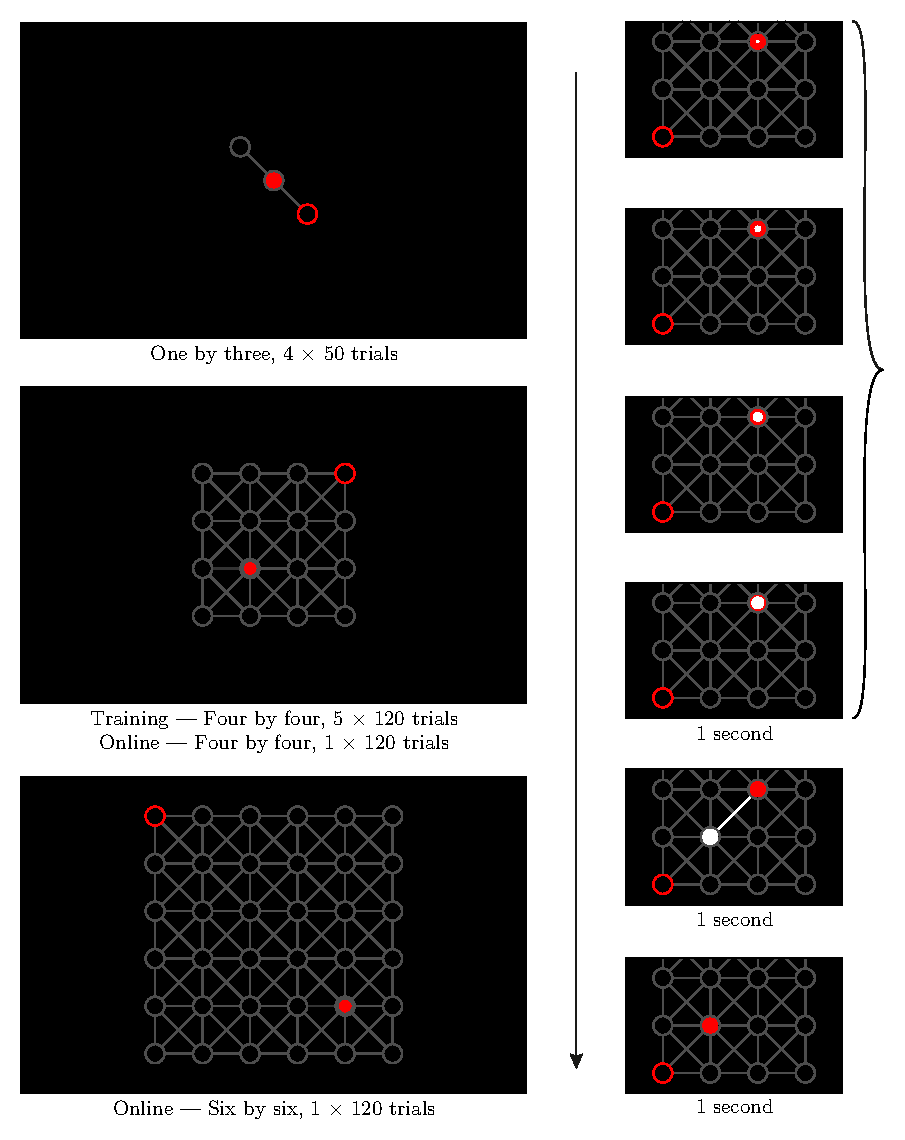
\includegraphics[width=\textwidth]{figures/nat-app-fig-s1.pdf}
    \caption[Experimental paradigm and procedure.]{Experimental Paradigm and Procedure. The experimental paradigm and procedure. \textit{Left}: Three different grid sizes were used in the experiment. Data from five blocks in 4$\times$4 grids was used to calibrate the classifier, which was then applied to another 4$\times$4 block, and one block on a 6$\times$6 grid. Data from the 1$\times$3 grids has not been used in this paper. Each cursor movement consisted of the cursor moving from one node to one of the directly adjacent ones. The cursor could move horizontally, vertically, and diagonally over the grid. Since the target was known and indicated, for each movement, it was possible to determine a measure of correctness for each movement by means of calculating the angular deviance, as in Supplementary Figure S2. \textit{Right}: Detail of a 4$\times$4 grid showing the cursor's movement animation.}
\end{figure}

\begin{figure}[t]
    \renewcommand\thefigure{\ref{chapter:nat}.S2}
    \centering
    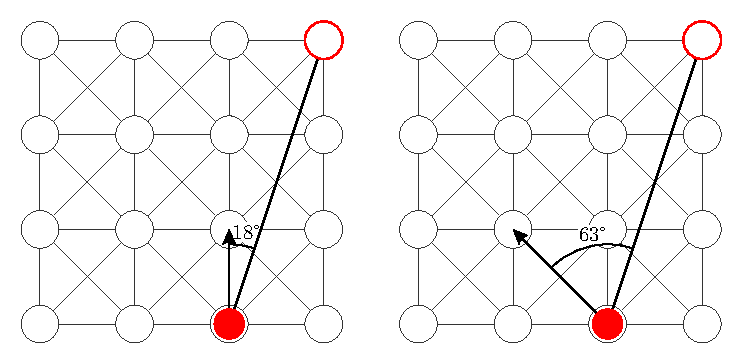
\includegraphics[scale=1.25]{figures/nat-app-fig-s2.pdf}
    \caption[Angular deviance.]{Angular Deviance. Illustration of the angular deviance of two possible cursor movements (north, and north-west) from the optimal path straight towards the target. Angular deviance was measured as the absolute deviation, in degrees, of the movement direction from a straight line to the target.}
\end{figure}

\begin{figure}[b]
    \renewcommand\thefigure{\ref{chapter:nat}.S3}
    \centering
    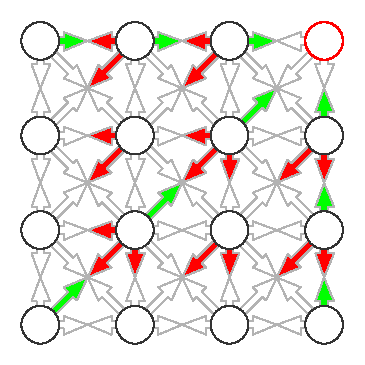
\includegraphics[scale=1.25]{figures/nat-app-fig-s3.pdf}
    \caption[Class definitions of the classifier's training set.]{Class Definition of the Classifier's Training Set. The classifier was calibrated on a subset of trials from a 600-trial calibration session. This set was selected by angular deviance: Movements with an absolute angular deviance to the target of 0º were included as `correct', while movements with a deviance of 135º or more were included as `incorrect'. This figure illustrates which of all possible movements on the 4$\times$4 grid were included, and in which category: Green represents `correct', red `incorrect'. From the total of 600 trials per participant on the 4$\times$4 grids, this selection left 62.7 ± 7.8 `correct' and 124.4 ± 8.9 `not accepable' trials per participant for the classifier to be calibrated on.}
\end{figure}

\begin{figure}[p]
    \renewcommand\thefigure{\ref{chapter:nat}.S4}
    \centering
    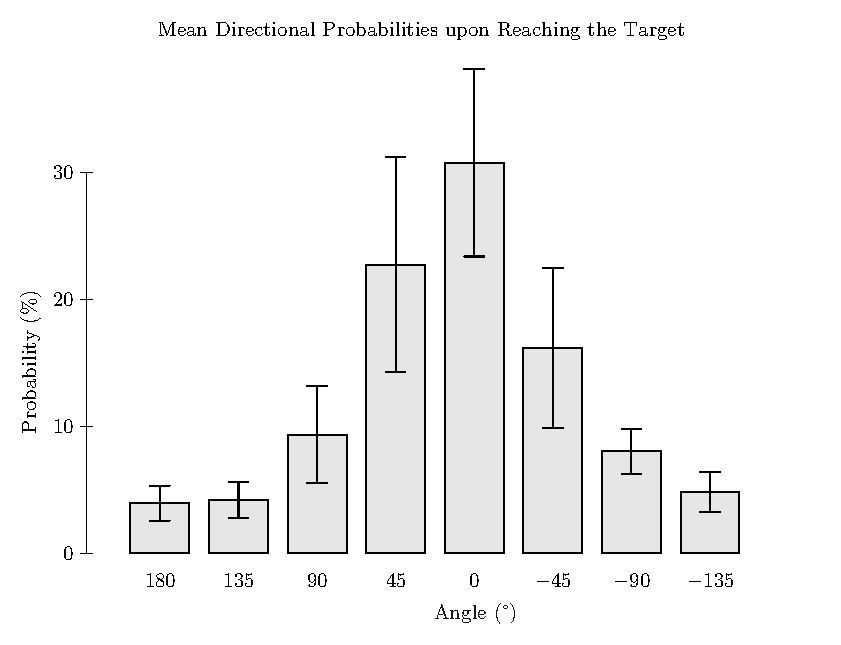
\includegraphics[width=\textwidth]{figures/nat-app-fig-s4.pdf}
    \caption[Mean directional probabilities upon hitting the target.]{Directional Probabilities. Mean directional probabilities, relative to the target from the cursor's starting position, upon hitting the target, in the BCI-supported condition, averaged over participants. Error bars represent the standard deviation. See Supplementary Table S2 for significance tests.}
\end{figure}

\begin{figure}[p]
    \renewcommand\thefigure{\ref{chapter:nat}.S5.1}
    \centering
    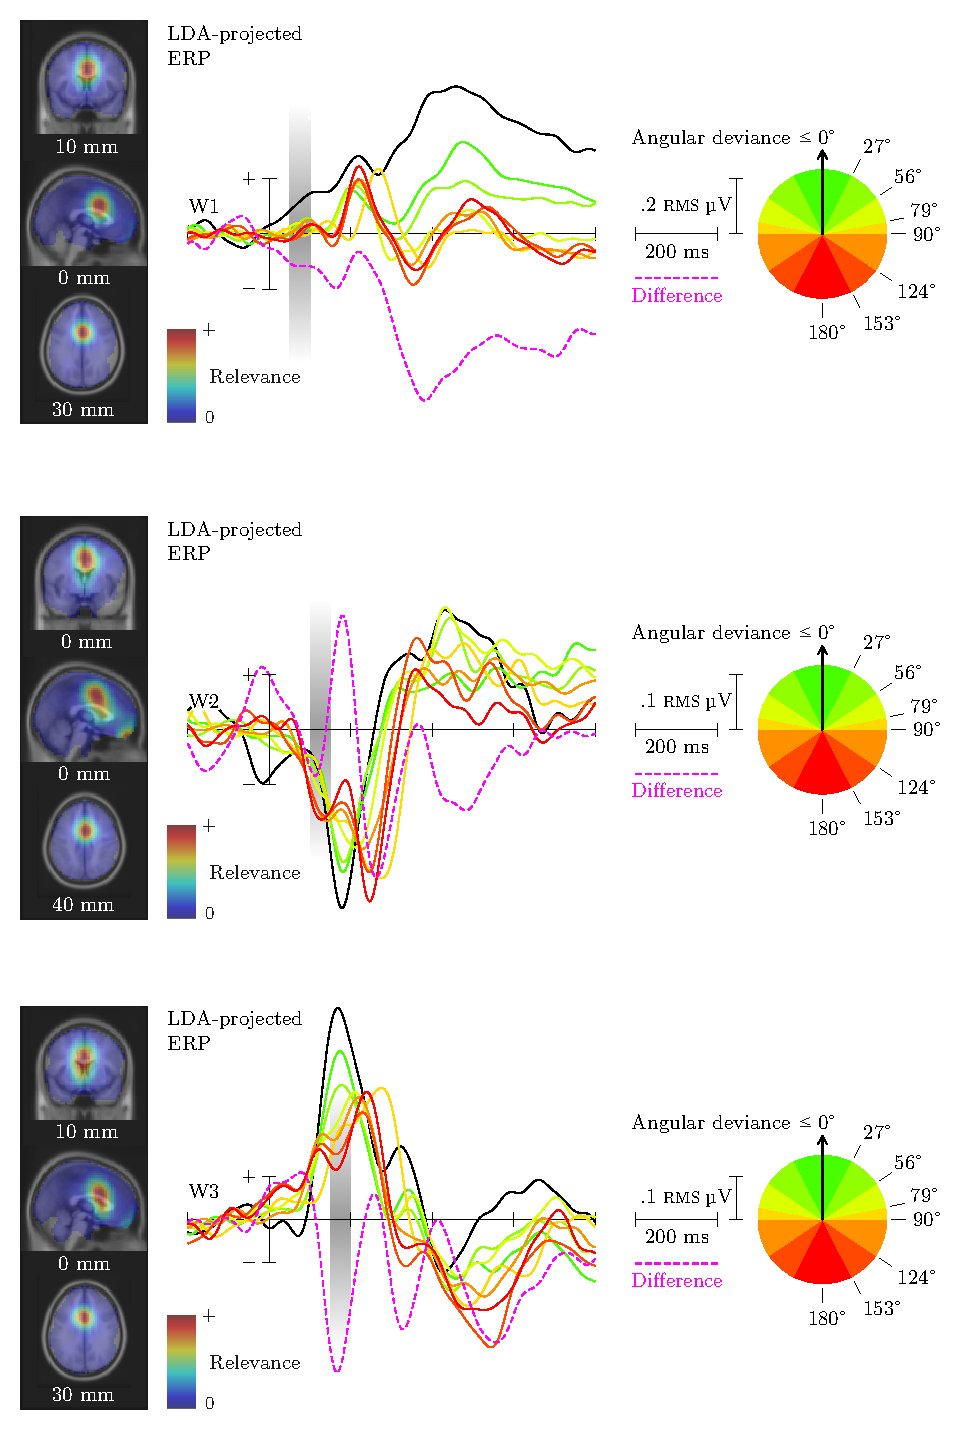
\includegraphics[width=\textwidth]{figures/nat-app-fig-s5-1.pdf}
    \caption{LDA-projected ERPs. (This figure spans three pages; this is page 1 of 3.)}
\end{figure}

\begin{figure}[p]
    \renewcommand\thefigure{\ref{chapter:nat}.S5.2}
    \centering
    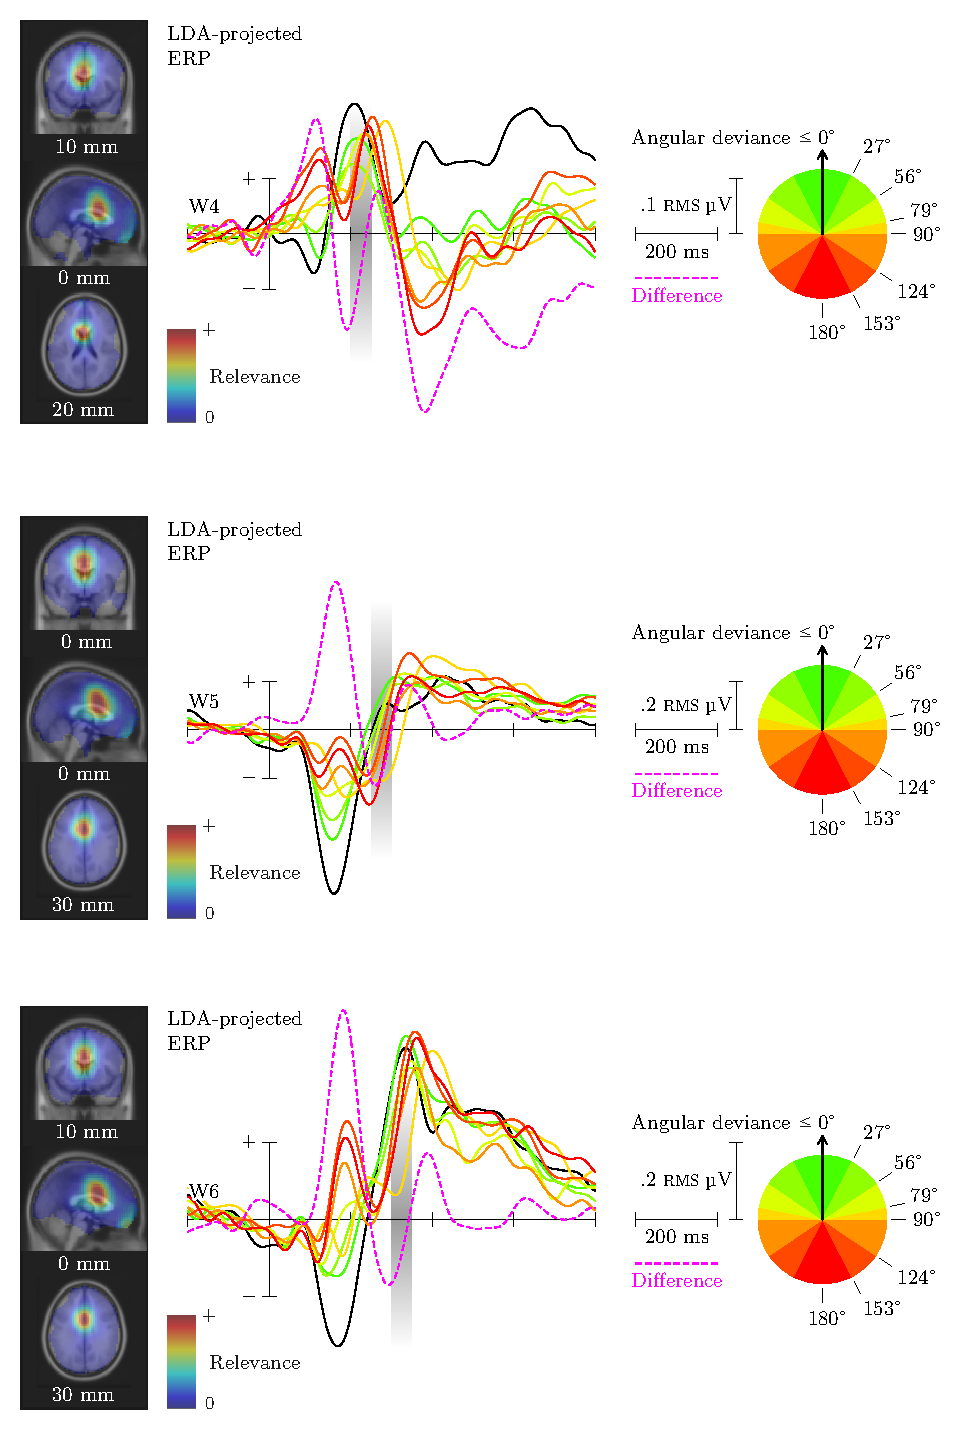
\includegraphics[width=\textwidth]{figures/nat-app-fig-s5-2.pdf}
    \caption{LDA-projected ERPs. (This figure spans three pages; this is page 1 of 3.)}
\end{figure}

\begin{figure}[p]
    \renewcommand\thefigure{\ref{chapter:nat}.S5.3}
    \centering
    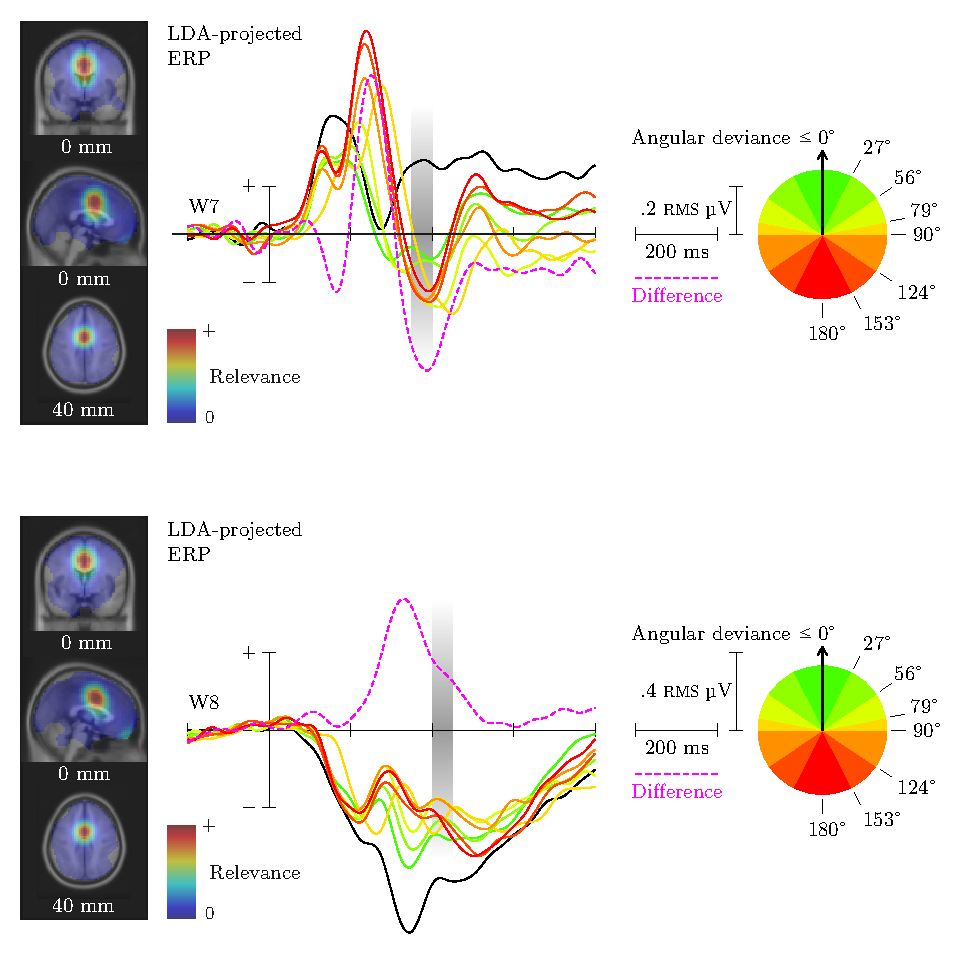
\includegraphics[width=\textwidth]{figures/nat-app-fig-s5-3.pdf}
    \caption[LDA-projected ERPs. (This figure spans three pages; this is page 1 of 3.)]{LDA-projected ERPs. (This figure spans three pages; this is page 1 of 3.) The classifier was calibrated on features spanning eight time windows of 50 ms each. For each time window, the above figures show on the left: Source localisation via weighted dipole density of the process(es) focused on in that time window; right: Full-length ERPs, combined as per that time window's LDA filter, of eight groups of cursor movement, as well as the projected difference wave between `correct' and `incorrect' classes (i.e. the filter's optimisation target). Each figure's actual time window, which actually contributed to classification, is highlighted in grey.}
\end{figure}

\begin{figure}[p]
    \renewcommand\thefigure{\ref{chapter:nat}.S6}
    \centering
    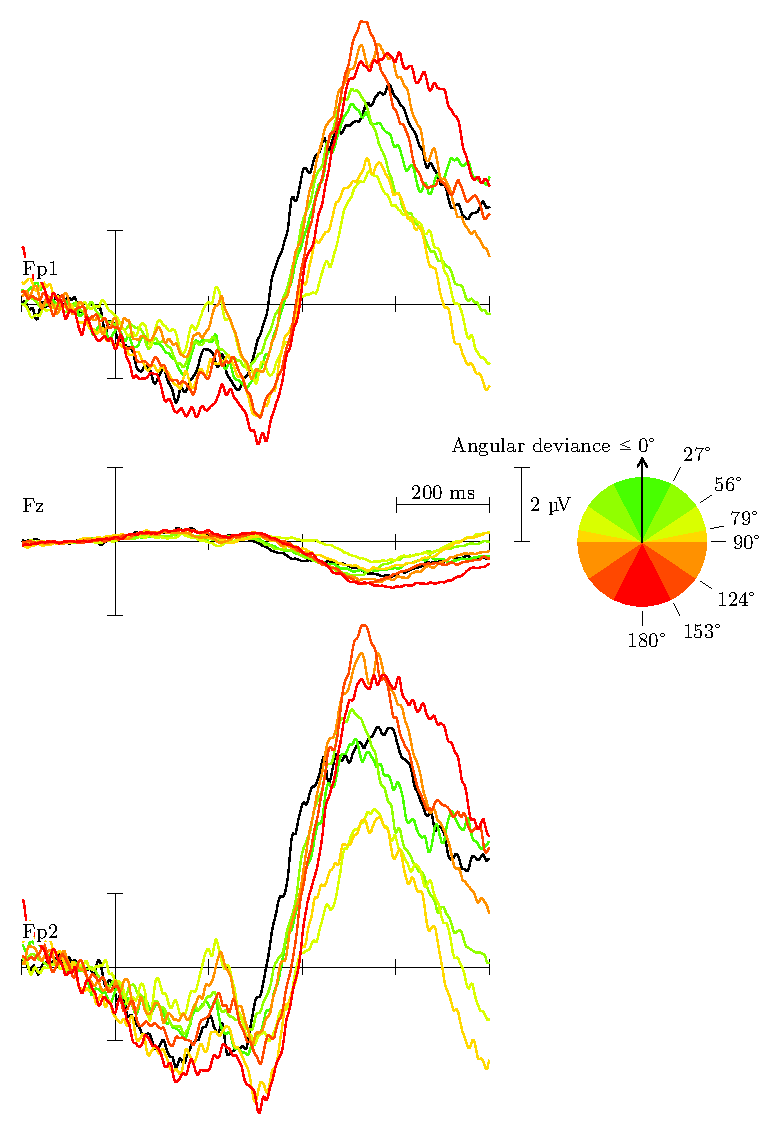
\includegraphics[width=\textwidth]{figures/nat-app-fig-s6.pdf}
    \caption[Influence of Eye Movements on the ERP at Fz.]{Influence of Eye Movements on the ERP at Fz. The grand average ERP (n = 19) at Fp1, Fp2, and Fz for only those components that contained strong eye movements and were removed for neurophysiological analysis. No systematic response is visible.}
\end{figure}

\begin{figure}[t]
    \renewcommand\thefigure{\ref{chapter:nat}.S7}
    \centering
    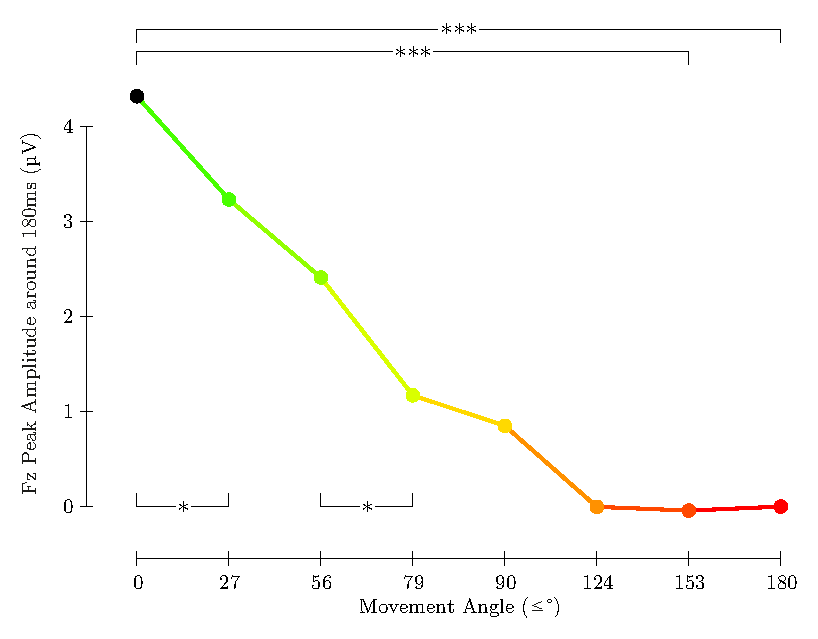
\includegraphics[scale=0.775]{figures/nat-app-fig-s7.pdf}
    \caption[Peak amplitudes around 180 ms for eight angular categories of cursor movements.]{Peak amplitudes around 180 ms for the eight groups of cursor movements. The peak amplitudes differ significantly (p < 0.001 ***) between the classes used by the classifier. In between, the peak amplitudes scale linearly with angular deviance, as fitted by a linear regression model using each group's mean angular deviance as predictor (b = -0.0035, F = 45.28, p < 0.001; R2 = 0.33). Statistically significant differences between adjacent groups are indicated as well (p < 0.05 *). See Supplementary Table S3 for exact figures of all comparisons. Classifier output followed a similar trend, as in Figure 1 of the manuscript.}
\end{figure}

\begin{figure}[b]
    \renewcommand\thefigure{\ref{chapter:nat}.S8}
    \centering
    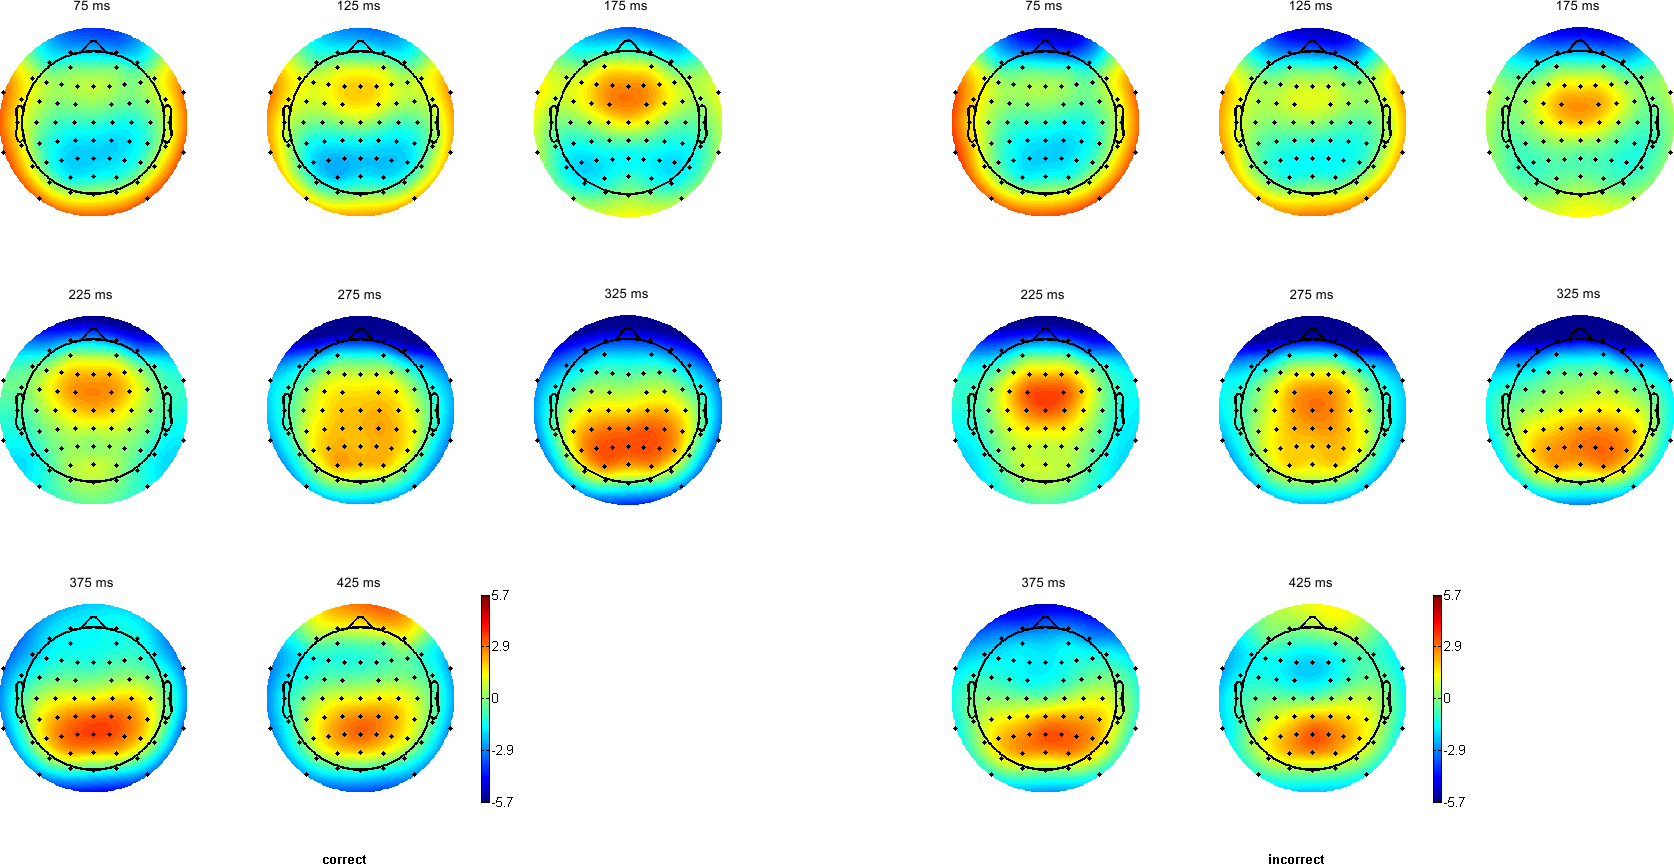
\includegraphics[width=\textwidth]{figures/nat-app-fig-s8.png}
    \caption[Scalp activity series time-locked to cursor movements.]{Scalp Activity Series. Class-specific grand average scalp activities (n = 19), time-locked to cursor movement, at the middle of each time of the eight time windows used for classification. \textit{Left:} Scalp activities of class 1, containing only cursor movements that went directly towards the target. \textit{Right:} Scalp activities of class 2, containing cursor movements with an angular deviance of 135$^\circ$ or more. EEG data was first band-pass filtered from 0.1 to 5 Hz as per the classification approach and re-referenced to the common average. See Figure 2 in the main manuscript and Supplementary Movie S1 for the class-correlated scalp activity that the classifier focused on.}
\end{figure}

\begin{figure}[p]
    \renewcommand\thefigure{\ref{chapter:nat}.S9}
    \centering
    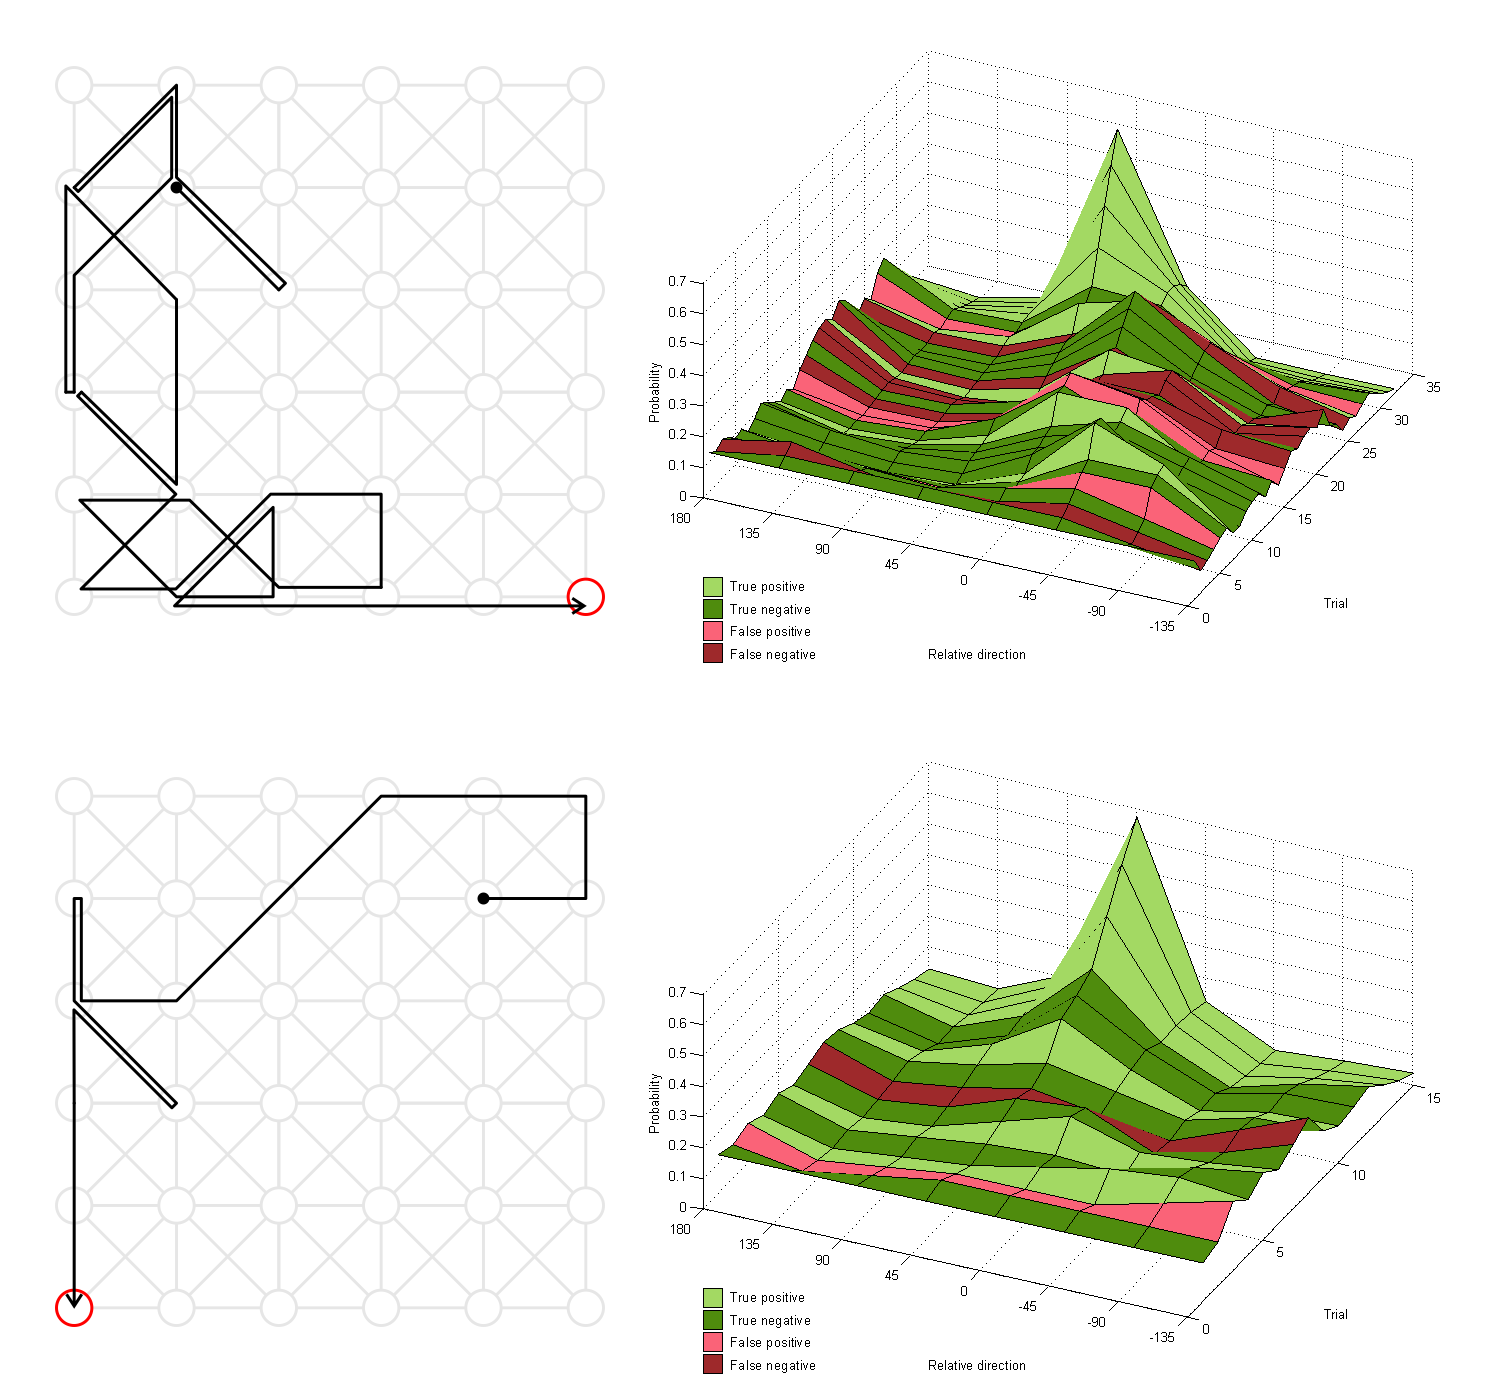
\includegraphics[width=\textwidth]{figures/nat-app-fig-s9.png}
    \caption[Example online cursor behavior.]{Example Online Cursor Behavior. Visualization of two online target selections. \textit{Left:} Trace of cursor movements over the grid. Each cursor movement only progressed one node over the grid; extended straight lines thus reflect multiple movements. \textit{Right:} Progression of normalized directional probabilities relative to 0º, with 0º being the direction towards the target at the start of the grid. All directions started out with equal probabilities, indicated at trial 0. Each subsequent trial shows the directional probabilities after that trial's cursor movement was classified and the cursor was reinforced accordingly. The colors reflect the confusion matrix with the participant's button presses being used as ground truth. True positive (light green) indicates the cursor movement was correctly classified as `correct'. True negative (dark green) indicates a correctly classified `incorrect' movement; false positive (light red) an incorrectly classified `correct' movement; false negative (dark red) an incorrectly classified `incorrect' movement. The top row shows a relatively slow online run of 31 trials on a six-by-six grid. A number of misclassifications, especially near the middle, delay the probabilistic model's convergence towards the desired target direction. However, the erroneous trials do not lead to an adverse bias while the correct classifications do systematically point towards the target, and the correct direction is found. The lower row shows a shorter run of 14 trials with only two misclassifications.}
\end{figure}

\begin{figure}[t]
    \renewcommand\thefigure{\ref{chapter:nat}.S10}
    \centering
    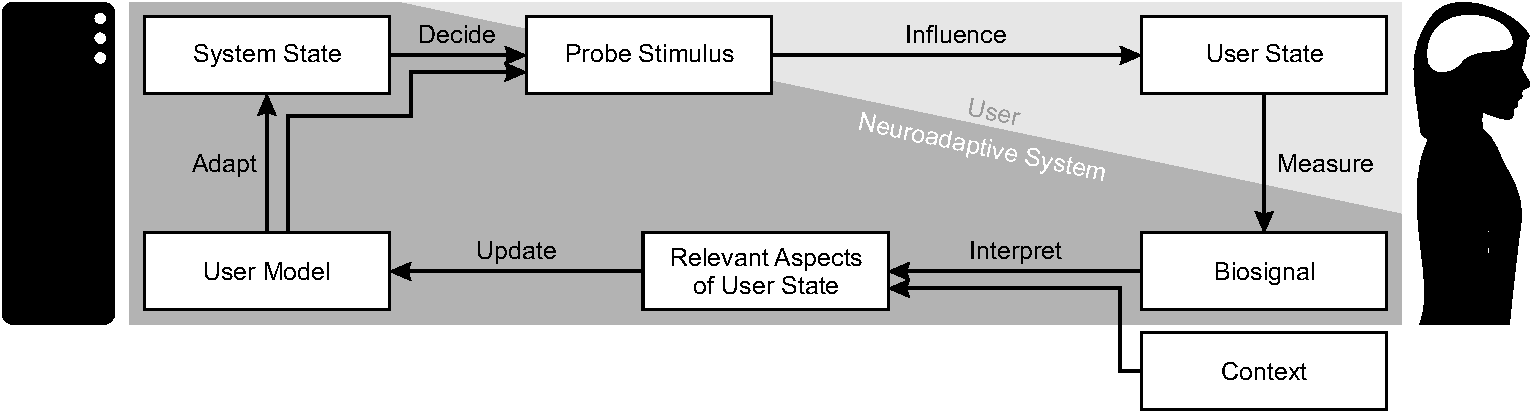
\includegraphics[width=\textwidth]{figures/nat-app-fig-s10.pdf}
    \caption[The neuroadaptive control loop.]{The neuroadaptive control loop. A stimulus or parameter change provokes an automatic response from the user, whose biosignals are monitored. The user's response can be classified from the gathered data, allowing the system to interpret the response in light of the previously gathered user information and the current context. With this information, the system updates its user model. Based on the user model and the current system status, the system may decide on a new probe stimulus.}
\end{figure}

\begin{table}[hb]
    \renewcommand\thetable{\ref{chapter:nat}.S1}
    \centering
    \small
    \begin{tabular}{ c | r r r | r r r}
        \hline \hline
        \multicolumn{1}{ c }{} & \multicolumn{3}{ c }{\textbf{4 $\times$ 4 Grids}} & \multicolumn{3}{ c }{\textbf{6 $\times$ 6 Grids}} \\
        \cline{2-7}
        Participant & TP & TN & \textbf{CR} & TP & TN & \textbf{CR} \\
        \hline \hline
        07 &  .91 & .86 & \textbf{.89} & $\cdot$ & $\cdot$ & $\cdot$ \\
        08 &  .91 & .60 & \textbf{.77} & $\cdot$ & $\cdot$ & $\cdot$ \\
        09 &  .81 & .53 & \textbf{.71} & $\cdot$ & $\cdot$ & $\cdot$ \\
        10 &  .83 & .79 & \textbf{.81} & .76 &  .75 & \textbf{.76} \\
        11 & 1.00 & .83 & \textbf{.93} & .88 & 1.00 & \textbf{.93} \\
        12 &  .83 & .63 & \textbf{.76} & .82 &  .64 & \textbf{.73} \\
        13 &  .67 & .47 & \textbf{.59} & .87 &  .38 & \textbf{.67} \\
        14 &  .75 & .63 & \textbf{.70} & .84 &  .36 & \textbf{.69} \\
        15 &  .82 & .69 & \textbf{.75} & .71 &  .82 & \textbf{.75} \\
        16 &  .52 & .50 & \textbf{.52} & .39 &  .10 & \textbf{.29} \\
        17 &  .58 & .62 & \textbf{.59} & .50 &  .68 & \textbf{.58} \\
        18 &  .67 & .62 & \textbf{.65} & .44 &  .53 & \textbf{.48} \\
        19 &  .80 & .67 & \textbf{.75} & .92 &  .65 & \textbf{.80} \\
        20 &  .71 & .80 & \textbf{.74} & .70 &  .62 & \textbf{.67} \\
        21 &  .88 & .56 & \textbf{.76} & .74 &  .45 & \textbf{.63} \\
        22 & . 60 & .67 & \textbf{.63} & .40 &  .50 & \textbf{.43} \\
        \hline \hline
        \textbf{Mean} & \textbf{.77} & \textbf{.65} & \textbf{.72} & \textbf{.69} & \textbf{.58} & \textbf{.65} \\
        \hline \hline
    \end{tabular}
    \caption[Online classification rates for cursor movements on two grid sizes.]]{Online classification rates for the 4$\times$4 grid, and the 6$\times$6  grid. TP = True Positives, TN = True Negatives, CR = Classification Rate (combined TP and TN). This table lists the classification rates for the online blocks, i.e. what percentage of classifier output agreed with the given definitions of `correct' and `incorrect' movements. These definitions were the same as the ones used for calibration: Movements with an angular deviance to the target of 0º were defined to be `correct', and those with a deviance of 135º or more were taken to be `incorrect'. The labels of all other movements were subject to individual interpretation, and have therefore not been included in this analysis. The table lists these rates for all participants that completed online blocks. From the total of nineteen, this excludes the first three participants, who only performed offline calibration blocks. A further three participants only performed 4$\times$4 grids online. }
\end{table}

\begin{table}[t]
    \renewcommand\thetable{\ref{chapter:nat}.S2}
    \centering
    \small
    \begin{tabular}{ r | r r r r r r r r }
        \hline \hline
        \multicolumn{1}{ c }{} & \multicolumn{7}{ c }{\textbf{Pairwise Comparison}} \\
        \multicolumn{1}{ c }{} & 180$^\circ$ & 135$^\circ$ & 90$^\circ$ & 45$^\circ$ & 0$^\circ$ & $-$45$^\circ$ & $-$90$^\circ$ \\
        \cline{2-8}
        135$^\circ$ & 1.000 & $\cdot$ & $\cdot$ & $\cdot$ & $\cdot$ & $\cdot$ & $\cdot$ \\
         90$^\circ$ &  0.004 & 0.003 & $\cdot$ & $\cdot$ & $\cdot$ & $\cdot$ & $\cdot$ \\
         45$^\circ$ &  0.000 & 0.000 & 0.000 & $\cdot$ & $\cdot$ & $\cdot$ & $\cdot$ \\
          0$^\circ$ &  0.000 & 0.000 & 0.000 & 1.000 & $\cdot$ &$\cdot$ & $\cdot$ \\
        $-$45$^\circ$ &  0.000 & 0.000 & 0.304 & 1.000 & 0.000 & $\cdot$ & $\cdot$ \\
        $-$90$^\circ$ &  0.000 & 0.000 & 1.000 & 0.000 & 0.000 & 0.006 & $\cdot$ \\
        $-$135$^\circ$ & 1.000 & 1.000 & 0.005 & 0.000 & 0.000 & 0.000 & 0.000 \\
        \hline \hline
    \end{tabular}
    \caption[Bonferroni-adjusted pairwise comparisons of the cursor's mean directional probabilities upon reaching the target.]{Bonferroni-adjusted pairwise comparisons of the mean directional probabilities upon reaching the target. Supplementary Figure S4 shows the mean directional probabilities upon reaching the target in both online grids, sorted by their angular deviance to the target, which was fixed relative to the cursor’s starting position. Supplementary Table S2 lists the Bonferroni-adjusted results of pairwise post-hoc tests from a one-way ANOVA (F(7,105) = 57.520, p < 0.001) on this data. On average, the classifier has been able to reinforce the ‘correct’ directions significantly more strongly than ‘incorrect’ directions.}
\end{table}

\begin{table}[b]
    \renewcommand\thetable{\ref{chapter:nat}.S3}
    \centering
    \small
    \begin{tabular}{ r | r r r r r r r r }
        \hline \hline
        \multicolumn{1}{ c }{} & \multicolumn{7}{ c }{\textbf{Pairwise Comparison}} \\
        \multicolumn{1}{ c }{} & $0^\circ$& $\leq27^\circ$ & $\leq56^\circ$ & $\leq79^\circ$ & $\leq90^\circ$ & $\leq124^\circ$ & $\leq153^\circ$ \\
        \cline{2-8}
        $\leq27^\circ$ & 0.032 & $\cdot$ & $\cdot$ & $\cdot$ & $\cdot$ & $\cdot$ & $\cdot$ \\
        $\leq56^\circ$ & 0.001 & 0.075 & $\cdot$ & $\cdot$ & $\cdot$ & $\cdot$ & $\cdot$ \\
        $\leq79^\circ$ & 0.000 & 0.000 & 0.020 & $\cdot$ & $\cdot$ & $\cdot$ & $\cdot$ \\ 
        $\leq90^\circ$ & 0.000 & 0.000 & 0.004 & 0.309 & $\cdot$ & $\cdot$ & $\cdot$ \\
        $\leq124^\circ$ & 0.000 & 0.000 & 0.000 & 0.023 & 0.071 & $\cdot$ & $\cdot$ \\
        $\leq153^\circ$ & 0.000 & 0.000 & 0.000 & 0.021 & 0.066 & 0.507 & $\cdot$ \\ 
        $\leq180^\circ$ & 0.000 & 0.000 & 0.000 & 0.023 & 0.071 & 0.520 & 0.531 \\
        \hline \hline
    \end{tabular}
    \caption[Pairwise comparisons, adjusted for false discovery rate, of the mean peak amplitudes at Fz for eight angular categories of cursor movements.]{Pairwise comparisons, adjusted for false discovery rate, of the mean peak amplitudes at Fz for the eight angular categories. A one-way ANOVA indicated a significant influence of angular deviance on peak amplitude (F(7,126) = 47.24, p < 0.001). In this table are listed the post-hoc comparisons---one-sided t-tests with pooled standard deviations, corrected for false discovery rate---between the eight individual groups of cursor movement.}
\end{table}

\clearpage

\begin{table}[t]
    \renewcommand\thetable{\ref{chapter:nat}.S4}
    \centering
    \small
    \begin{tabular}{ r | r r r r r r r r }
        \hline \hline
        \multicolumn{1}{ c }{} & \multicolumn{7}{ c }{\textbf{Pairwise Comparison}} \\
        \multicolumn{1}{ c }{} & $0^\circ$& $\leq27^\circ$ & $\leq56^\circ$ & $\leq79^\circ$ & $\leq90^\circ$ & $\leq124^\circ$ & $\leq153^\circ$ \\
        \cline{2-8}
        $\leq27^\circ$ & 0.328 & $\cdot$ & $\cdot$ & $\cdot$ & $\cdot$ & $\cdot$ & $\cdot$ \\
        $\leq56^\circ$ & 0.000 & 0.002 & $\cdot$ & $\cdot$ & $\cdot$ & $\cdot$ & $\cdot$ \\
        $\leq79^\circ$ & 0.000 & 0.000 & 0.023 & $\cdot$ & $\cdot$ & $\cdot$ & $\cdot$ \\ 
        $\leq90^\circ$ & 0.000 & 0.000 & 0.000 & 0.115 & $\cdot$ & $\cdot$ & $\cdot$ \\
        $\leq124^\circ$ & 0.000 & 0.000 & 0.000 & 0.006 & 0.125 & $\cdot$ & $\cdot$ \\
        $\leq153^\circ$ & 0.000 & 0.000 & 0.000 & 0.308 & 0.311 & 0.829 & $\cdot$ \\ 
        $\leq180^\circ$ & 0.000 & 0.000 & 0.000 & 0.311 & 0.829 & 0.979 & 0.952 \\
        \hline \hline
    \end{tabular}
    \caption[Pairwise comparisons, adjusted for false discovery rate, of the mean classifier output for eight angular categories of cursor movements.]{Pairwise comparisons, adjusted for false discovery rate, of the mean classifier output for the eight angular categories. A one-way ANOVA indicated a significant influence of angular deviance on classifier output (F(7,105) = 28.32, p < 0.001). In this table are listed the post-hoc comparisons---one-sided t-tests with pooled standard deviations, corrected for false discovery rate---between the eight individual groups of cursor movement.}
\end{table}

\begin{table}[b]
    \renewcommand\thetable{\ref{chapter:nat}.S5}
    \centering
    \small
    \begin{tabular}{ r | r r r r r r r r }
        \hline \hline
        \multicolumn{1}{ c }{} & \multicolumn{7}{ c }{\textbf{Pairwise Comparison}} \\
        \multicolumn{1}{ c }{} & $0^\circ$& $\leq27^\circ$ & $\leq56^\circ$ & $\leq79^\circ$ & $\leq90^\circ$ & $\leq124^\circ$ & $\leq153^\circ$ \\
        \cline{2-8}
        $\leq27^\circ$ & 0.004 & $\cdot$ & $\cdot$ & $\cdot$ & $\cdot$ & $\cdot$ & $\cdot$ \\
        $\leq56^\circ$ & 0.000 & 0.007 & $\cdot$ & $\cdot$ & $\cdot$ & $\cdot$ & $\cdot$ \\
        $\leq79^\circ$ & 0.000 & 0.000 & 0.009 & $\cdot$ & $\cdot$ & $\cdot$ & $\cdot$ \\ 
        $\leq90^\circ$ & 0.000 & 0.000 & 0.000 & 0.093 & $\cdot$ & $\cdot$ & $\cdot$ \\
        $\leq124^\circ$ & 0.000 & 0.000 & 0.000 & 0.168 & 0.599 & $\cdot$ & $\cdot$ \\
        $\leq153^\circ$ & 0.000 & 0.000 & 0.000 & 0.014 & 0.161 & 0.134 & $\cdot$ \\ 
        $\leq180^\circ$ & 0.000 & 0.000 & 0.000 & 0.004 & 0.046 & 0.404 & 0.227 \\
        \hline \hline
    \end{tabular}
    \caption[Pairwise comparisons of the mean amplitudes in the third time window (150-200 ms) of the LDA-projected ERP.]{Pairwise comparisons of the mean amplitudes in the third time window (150-200 ms) of the LDA-projected ERP. Supplementary Figure S5 shows LDA-projected ERPs. At Fz, significant amplitude differences were found at around 180 ms following cursor onset (see Figure 1 of the main manuscript and Supplementary Figure S7). This falls within the third time window used by the classification system (150 to 200 ms following cursor movement). This table shows the results of pairwise comparisons using one-tailed permutation tests of the mean amplitudes of the LDA-projected ERPs in that time window, between the eight individual groups of cursor movement.}
\end{table}

\begin{figure}[t]
    \renewcommand\thefigure{\ref{chapter:nat}.M1}
    \centering
    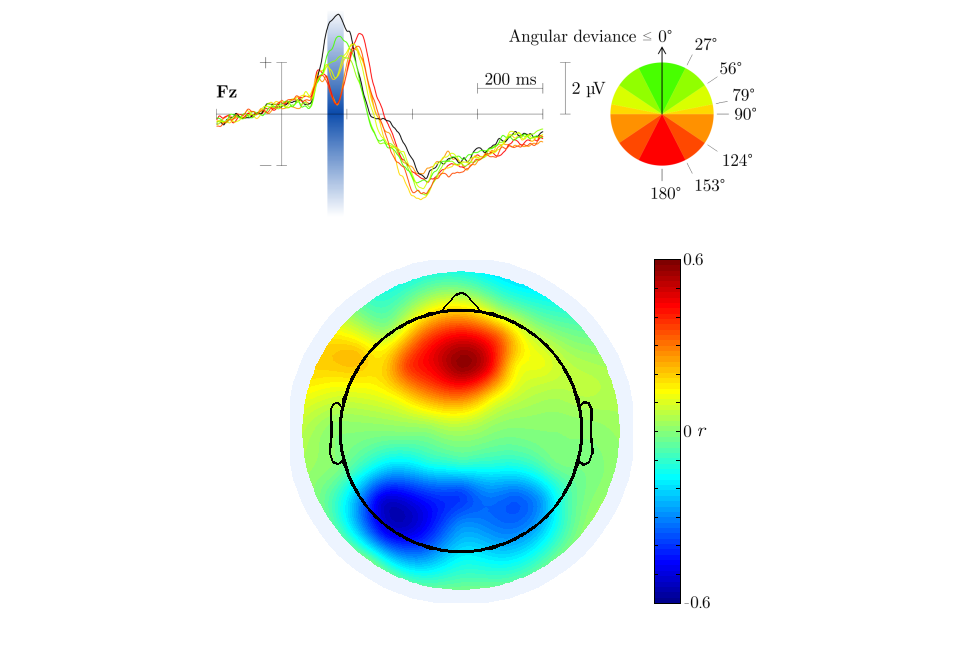
\includegraphics[width=0.9\textwidth]{figures/nat-app-movie-s1-still.png}
    \caption[Movie S1. Event-related potential at electrode Fz, and class-correlated scalp activity derived from the LDA filter weights of sequential 50-ms time windows,
spanning the 400 ms used for classification.]{Movie S1. Event-related potential at electrode Fz, and class-correlated scalp activity derived from the LDA filter weights of sequential 50-ms time windows,
spanning the 400 ms used for classification. Available online at \href{https://doi.org/10.1073/pnas.1605155114}{https://doi.org/10.1073/pnas.1605155114}}
\end{figure}

\begin{figure}[b]
    \renewcommand\thefigure{\ref{chapter:nat}.M2}
    \centering
    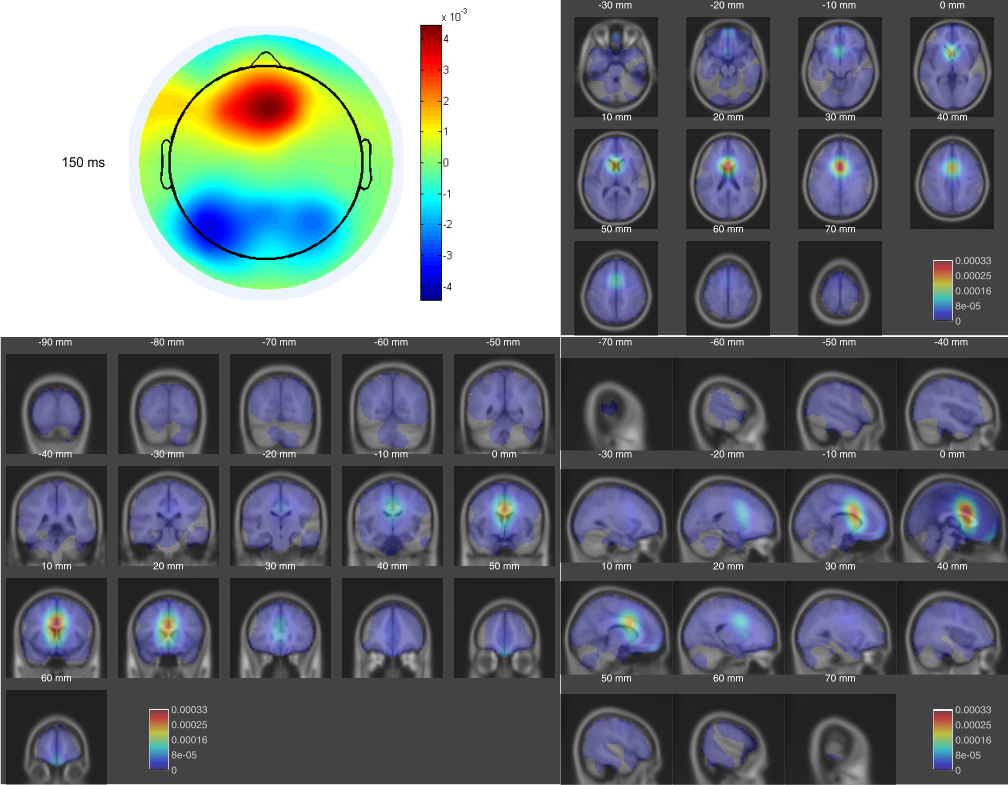
\includegraphics[width=0.8\textwidth]{figures/nat-app-movie-s2-still.png}
    \caption[Movie S2. Dipole densities weighted by relevance for classification in sequential 50-ms time windows, spanning the 400 ms used for classification.]{Movie S2. Dipole densities weighted by relevance for classification in sequential 50-ms time windows, spanning the 400 ms used for classification. Available online at \href{https://doi.org/10.1073/pnas.1605155114}{https://doi.org/10.1073/pnas.1605155114}}
\end{figure}

\begin{figure}[t]
    \renewcommand\thefigure{\ref{chapter:nat}.M3}
    \centering
    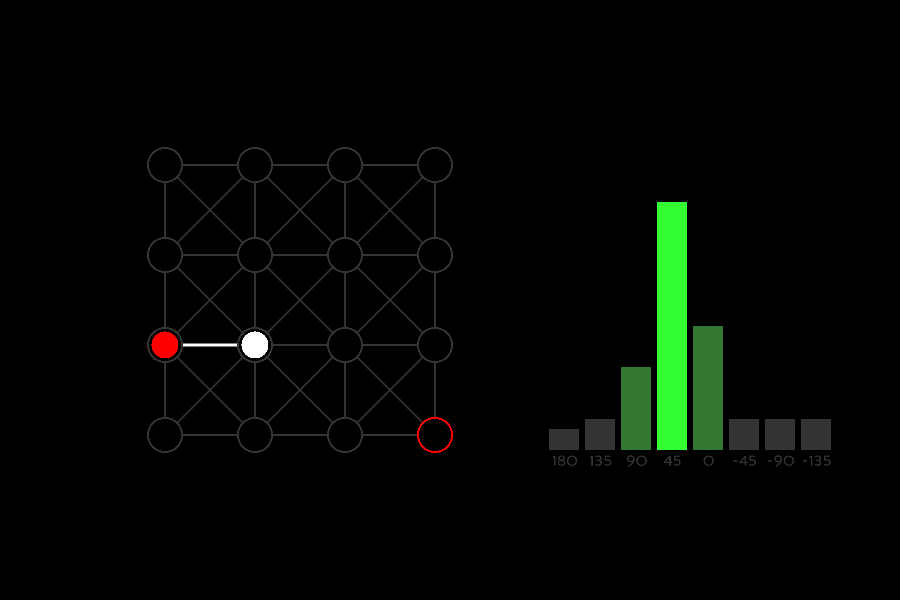
\includegraphics[width=0.9\textwidth]{figures/nat-app-movie-s3-still.png}
    \caption[Movie S3. Online experimental stimuli accompanied by classification output, illustrating the online process and outcome.]{Movie S3. Online experimental stimuli accompanied by classification output, illustrating the online process and outcome. \\ Available online at \href{https://doi.org/10.1073/pnas.1605155114}{https://doi.org/10.1073/pnas.1605155114}}
\end{figure}

\begin{figure}[b]
    \renewcommand\thefigure{\ref{chapter:nat}.M4}
    \centering
    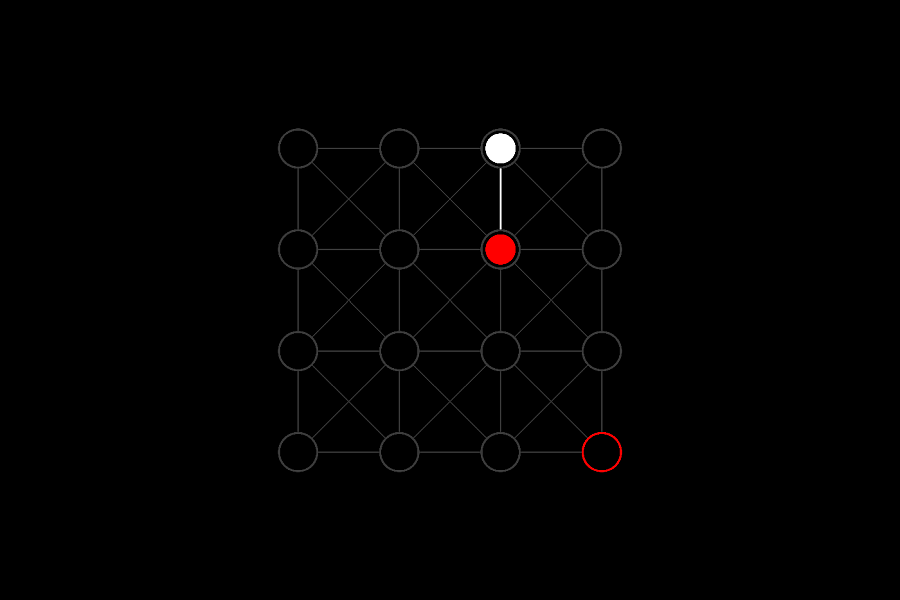
\includegraphics[width=0.9\textwidth]{figures/nat-app-movie-s4-still.png}
    \caption[Movie S4. Offline experimental stimuli.]{Movie S4. Offline experimental stimuli. \\ Available online at \href{https://doi.org/10.1073/pnas.1605155114}{https://doi.org/10.1073/pnas.1605155114}}
\end{figure}
    
\chapter*{Chapter \ref{chapter:salval} Supplementary Information}
\chaptermark{Chapter \ref{chapter:salval} Supplementary Information}
\addcontentsline{toc}{chapter}{Chapter \ref{chapter:salval} Supplementary Information}

\vfill

\begin{figure}[h]
    \renewcommand\thefigure{\ref{chapter:salval}.S1}
    \centering
    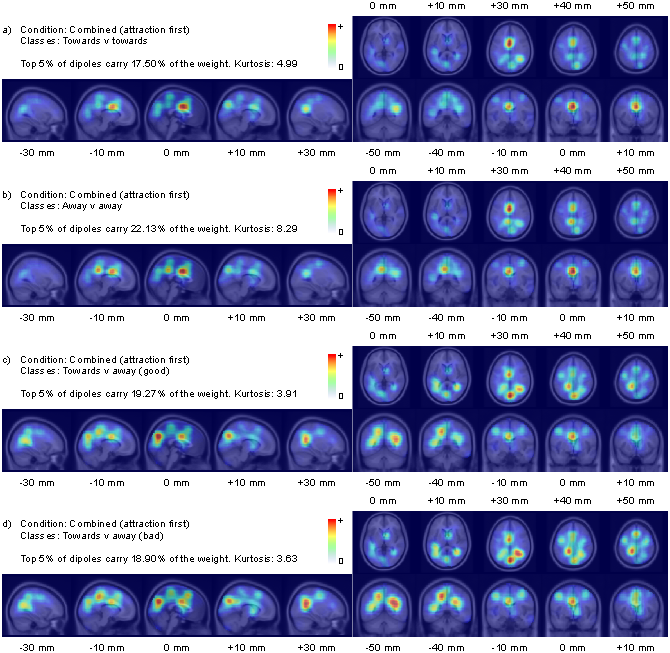
\includegraphics[width=\textwidth]{figures/salval-posfirst-wdd-combined-separate.pdf}
    \caption[Weighted dipole density plots for the two valence-focused and salience focused-classifiers separately, for the attraction-first group.]{Weighted dipole density plots showing the relevance of cortical areas to the two valence-focused and two salience-focused classifiers separately: \emph{a} TvT, \emph{b} AvA, \emph{c} TvT+ and \emph{d} TvT--, all for the attraction-first group.}
    \label{fig:posfirst-wdd-combined-separate}
\end{figure}

\vfill\null\clearpage

\null\vspace{55pt}

\vfill

\begin{figure}[h]
    \renewcommand\thefigure{\ref{chapter:salval}.S2}
    \centering
    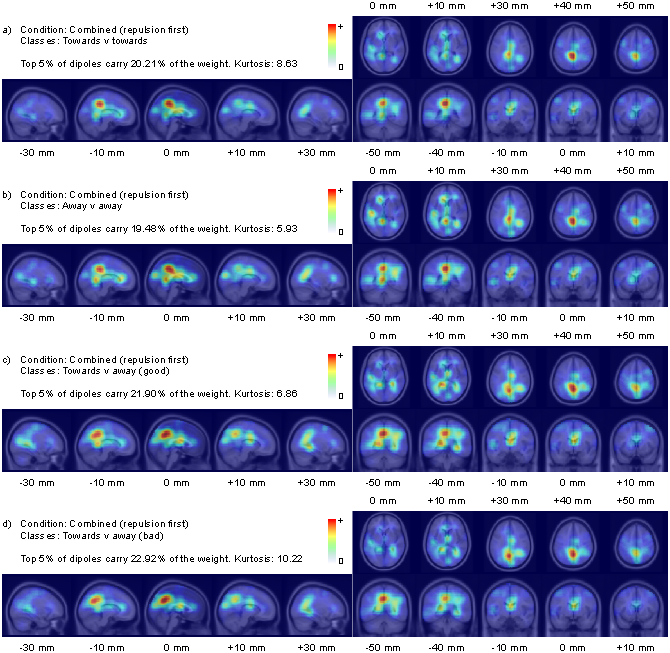
\includegraphics[width=\textwidth]{figures/salval-negfirst-wdd-combined-separate.pdf}
    \caption[Weighted dipole density plots for the two valence-focused and salience focused-classifiers separately, for the repulsion-first group.]{Weighted dipole density plots showing the relevance of cortical areas to the two valence-focused and two salience-focused classifiers separately: \emph{a} TvT, \emph{b} AvA, \emph{c} TvT+ and \emph{d} TvT--, all for the repulsion-first group.}
    \label{fig:negfirst-wdd-combined-separate}
\end{figure}

\vfill\null

\end{document}
